\chapter{Four materials problem}
The four materials problem is a two-dimensional transient conduction problem. It consists in a long rod composed of four different materials with different properties. The general scheme of the problem is represented in figure \ref{fourmaterials}, and the dimensions of the materials, their properties, and the boundary conditions are in the tables below.
\begin{figure}[H]
	\centering
	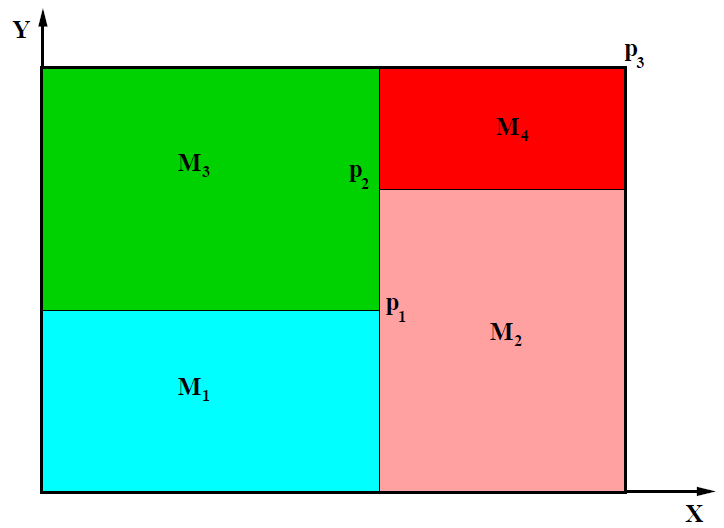
\includegraphics[scale = 0.6]{FourMaterials/Fourmaterials}
	\caption{General scheme of the four materials problem}
	\label{fourmaterials}
\end{figure}
\begin{table}[h!]
	\centering
	\begin{tabular}{ |c|c|c|}
		\hline
		  & x [m] & y [m] \\ \hline
		 $p_{1}$ & $0.50$ & $0.40$ \\ \hline
		 $p_{2}$ & $0.50$ & $0.70$ \\ \hline
		 $p_{3}$ & $1.10$ & $0.80$ \\ \hline
	\end{tabular}
\caption{Problem coordinates}
\end{table}
\begin{table}[h!]
	\centering
	\begin{tabular}{ |c|c|c|c| }
		\hline
		& $\rho [kg/m^{3}]$ & $c_{P} [J/kgK]$ & $\lambda [W/mK]$ \\ \hline
		$M_{1}$ & $1500.00$ & $750.00$ & $170.00$ \\ \hline
		$M_{2}$ & $1600.00$ & $770.00$ & $140.00$ \\ \hline
		$M_{3}$ & $1900.00$ & $810.00$ & $200.00$ \\ \hline
		$M_{4}$ & $2500.00$ & $930.00$ & $140.00$ \\ \hline
	\end{tabular}
\caption{Physical properties of the materials}
\end{table}
\begin{table}
	\centering
	\begin{tabular}{ |c|c|}
		\hline
		Cavity wall & Boundary condition \\ \hline
		Bottom & Isotherm at $T=23.00 ^{\circ}C$ \\ \hline
		Top & Uniform $Q_{flow}=60.00 W/m$ length \\ \hline
		Left & In contact with a fluid at $T_{g}=33.00 ^{\circ}C$ and heat transfer coefficient $9.00 W/m^{2}K$ \\ \hline
		Right & Uniform temperature $T=8.00+0.005t ^{\circ}C$ (where $t$ is the time in seconds) \\ \hline
	\end{tabular}
\caption{Boundary conditions}
\end{table}
Since it is a transient problem, it is necessary to know the temperature at $t=0$. The initial temperature field is $T=8.00 ^{\circ}C$.

\section{Discretization}
The spatial discretization of the problem is that described in section \ref{SpatialDiscretizationConduction}. However, since there are different materials, each of them is discretized separately. The variable $M_{1}$ is the number of control volumes in the vertical direction from $Y=0$ to the point $p_{1}$, $M_{2}$ from $p_{1}$ to $p_{2}$ and $M_{3}$ form $p_{2}$ to $p_{3}$. In the horizontal direction, the variable $N_{1}$ is the number of control volumes from $X=0$ to the point $p_{1}$ and $N_{2}$ from $p_{1}$ to $p_{3}$. The precision used in the convergence criterion is given by $\delta$.
\begin{table}[h]
	\centering
	\begin{tabular}{ |c|c|c|c|c|c|c| }
		\hline
		$M_{1}$ & $M_{2}$ & $M_{3}$ & $N_{1}$ & $N_{2}$ & $\beta$ & $\delta$ \\ \hline
		$40$ & $30$ & $10$ & $50$ & $60$ & $0.5$ & $10^{-3}$ \\ \hline
	\end{tabular}
	\caption{Numerical parameters of the four materials problem}
\end{table}

\section{Boundary conditions}
The coefficients of the discretized equation in the inner nodes are the ones of the section \ref{DiscrCond}. However, the outer walls of the rod have special conditions, so each of them has to be studied in order to determine which coefficients of their boundary nodes are different.

In the left wall, there is convection with the fluid outside of the road. To fulfil this condition, some coefficients have to be recalculated:
\begin{equation}
a_{W}=0
\end{equation}
\begin{equation}
a_{P}=a_{E}+a_{W}+a_{N}+a_{S}+\frac{\rho_{P}V_{P}\bar{c}_{P}}{\Delta t}+\frac{\beta}{\frac{1}{\alpha}+\frac{d_{Pw}}{\lambda_{P}}}
\end{equation}
\begin{multline}
b_{P}=\frac{\rho_{P}V_{P}\bar{c}_{P}T_{P}^{n}}{\Delta t}+\beta\left(\dot{q}_{vP}^{n+1}V_{P}+\frac{T_{g}}{\frac{1}{\alpha}+\frac{d_{Pw}}{\lambda_{P}}}\right) \\
+\left(1-\beta\right)\left[\frac{T_{g}-T_{P}}{\frac{1}{\alpha}+\frac{d_{Pw}}{\lambda_{P}}}+\lambda_{e}\frac{T_{E}-T_{P}}{d_{PE}}S_{e}-\lambda_{s}\frac{T_{P}-T_{S}}{d_{PS}}S_{s}+\lambda_{n}\frac{T_{N}-T_{P}}{d_{PN}}S_{n}+\dot{q}_{vP}V_{P}\right]^{n}
\end{multline}

There is a constant heat flux in the top wall. The value of this flux is given for the total wall, so it is assumed that it is uniformly distributed over the top wall. In this case, the coefficients that change their value are:
\begin{equation}
a_{N}=0
\end{equation}
\begin{multline}
b_{P}=\frac{\rho_{P}V_{P}\bar{c}_{P}T_{P}^{n}}{\Delta t}+\beta\dot{q}_{vP}^{n+1}V_{P}+Q_{flow}\frac{S_{n}}{S_{top}} \\
+\left(1-\beta\right)\left[-\lambda_{w}\frac{T_{P}-T_{W}}{d_{PW}}S_{w}+\lambda_{e}\frac{T_{E}-T_{P}}{d_{PE}}S_{e}-\lambda_{s}\frac{T_{P}-T_{S}}{d_{PS}}S_{s}+\dot{q}_{vP}V_{P}\right]^{n}
\end{multline}

In the right wall, the temperature $T_{r}$ is given, and it changes over time. The coefficients are very similar to those of the general case. The only differences are:
\begin{equation}
a_{E}=0
\end{equation}
\begin{equation}
a_P=a_{E}+a_{W}+a_{N}+a_{S}+\frac{\rho_{P}V_{P}\bar{c}_{P}}{\Delta t}+\beta\frac{\lambda_{P}S_{e}}{d_{Pe}}
\end{equation}
\begin{multline}
b_{P}=\frac{\rho_{P}V_{P}\bar{c}_{P}T_{P}^{n}}{\Delta t}+\beta\left(\dot{q}_{vP}^{n+1}V_{P}+\frac{\lambda_{P}S_{e}}{d_{Pe}}T_{r}^{n+1}\right) \\
+\left(1-\beta\right)\left[-\lambda_{w}\frac{T_{P}-T_{W}}{d_{PW}}S_{w}+\lambda_{P}\frac{T_{r}-T_{P}}{d_{Pe}}S_{e}-\lambda_{s}\frac{T_{P}-T_{S}}{d_{PS}}S_{s}+\lambda_{n}\frac{T_{N}-T_{P}}{d_{PN}}S_{n}+\dot{q}_{vP}V_{P}\right]^{n}
\end{multline}

Finally, in the bottom wall, the temperature $T_{b}$ is also given, but it is constant over time. The approach is very similar to that of the right wall, so that the different coefficients are:
\begin{equation}
a_{S}=0
\end{equation}
\begin{equation}
a_P=a_{E}+a_{W}+a_{N}+a_{S}+\frac{\rho_{P}V_{P}\bar{c}_{P}}{\Delta t}+\beta\frac{\lambda_{P}S_{s}}{d_{Ps}}
\end{equation}
\begin{multline}
b_{P}=\frac{\rho_{P}V_{P}\bar{c}_{P}T_{P}^{n}}{\Delta t}+\beta\left(\dot{q}_{vP}^{n+1}V_{P}+\frac{\lambda_{P}S_{s}}{d_{Ps}}T_{b}\right) \\
+\left(1-\beta\right)\left[-\lambda_{w}\frac{T_{P}-T_{W}}{d_{PW}}S_{w}+\lambda_{e}\frac{T_{E}-T_{P}}{d_{PE}}S_{e}-\lambda_{P}\frac{T_{P}-T_{b}}{d_{Ps}}S_{s}+\lambda_{n}\frac{T_{N}-T_{P}}{d_{PN}}S_{n}+\dot{q}_{vP}V_{P}\right]^{n}
\end{multline}

\section{Algorithm}
The algorithm used in this convection problem is represented below. In this case, some of the discretization coefficients are constant, but they usually change over time. These would change slightly the algorithm used.
\begin{figure}[h!]
	\centering
	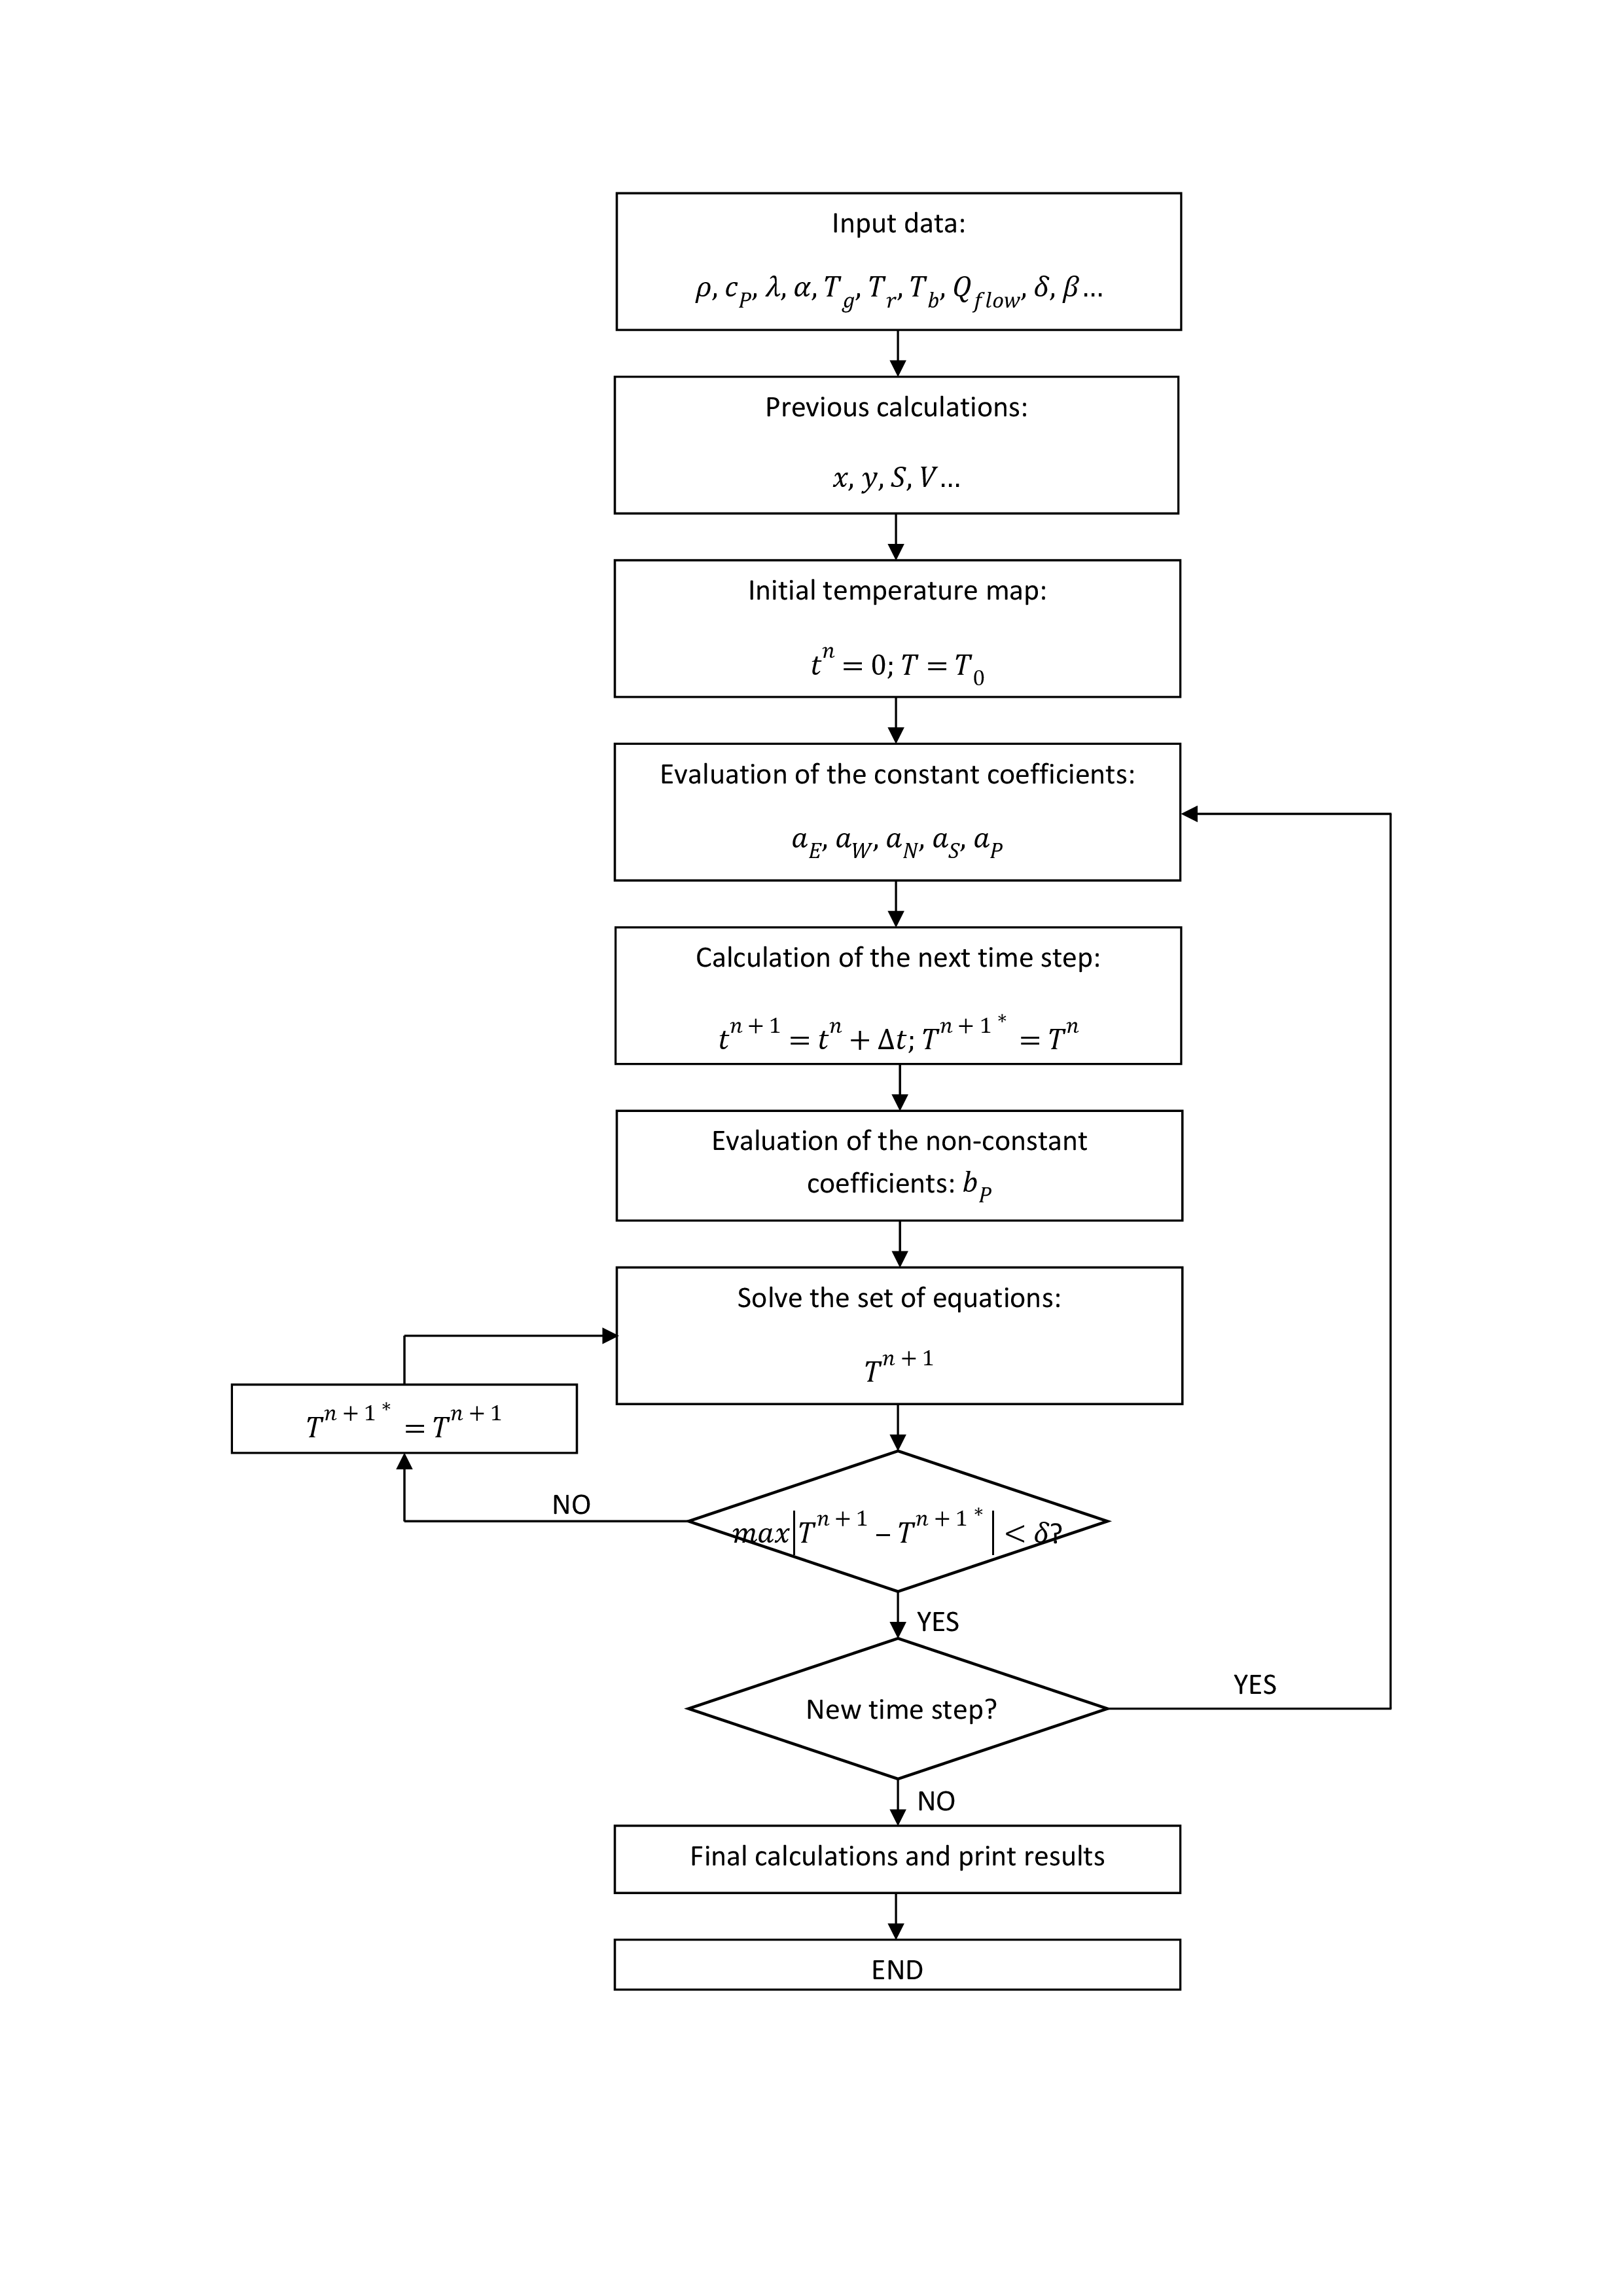
\includegraphics[scale=0.154]{FourMaterials/algorithm}
\end{figure}

\section{Results}
To verify the simulation, the results obtained are compared with the reference values for a time of t=5000 s. As it can be seen in figures \ref{ref4M} and \ref{ref4M}, the results of the code are very similar to the reference values. The biggest differences are the isotherms of $23$ and $24^{\circ}$.
\begin{figure}[h!]
	\centering
	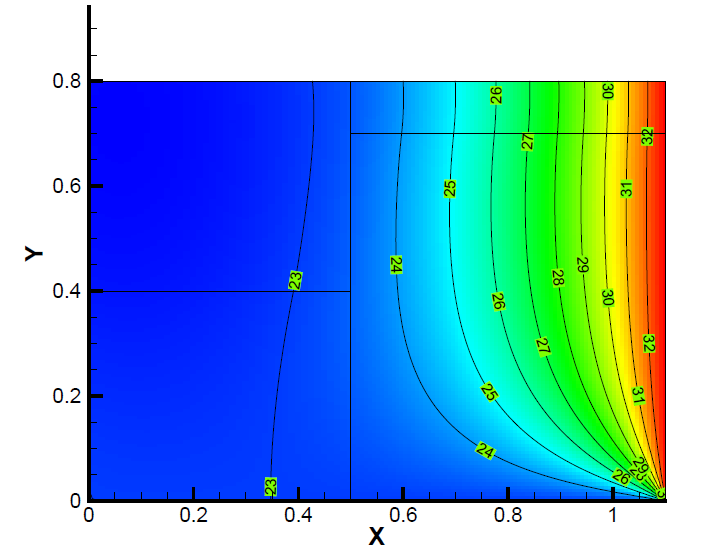
\includegraphics[scale=0.55]{FourMaterials/reference}
	\caption{Reference value: Instantaneous isotherms at t=10000/2 s}
	\label{ref4M}
\end{figure}
\begin{figure}[h!]
	\centering
	% GNUPLOT: LaTeX picture with Postscript
\begingroup
  \makeatletter
  \providecommand\color[2][]{%
    \GenericError{(gnuplot) \space\space\space\@spaces}{%
      Package color not loaded in conjunction with
      terminal option `colourtext'%
    }{See the gnuplot documentation for explanation.%
    }{Either use 'blacktext' in gnuplot or load the package
      color.sty in LaTeX.}%
    \renewcommand\color[2][]{}%
  }%
  \providecommand\includegraphics[2][]{%
    \GenericError{(gnuplot) \space\space\space\@spaces}{%
      Package graphicx or graphics not loaded%
    }{See the gnuplot documentation for explanation.%
    }{The gnuplot epslatex terminal needs graphicx.sty or graphics.sty.}%
    \renewcommand\includegraphics[2][]{}%
  }%
  \providecommand\rotatebox[2]{#2}%
  \@ifundefined{ifGPcolor}{%
    \newif\ifGPcolor
    \GPcolortrue
  }{}%
  \@ifundefined{ifGPblacktext}{%
    \newif\ifGPblacktext
    \GPblacktexttrue
  }{}%
  % define a \g@addto@macro without @ in the name:
  \let\gplgaddtomacro\g@addto@macro
  % define empty templates for all commands taking text:
  \gdef\gplbacktext{}%
  \gdef\gplfronttext{}%
  \makeatother
  \ifGPblacktext
    % no textcolor at all
    \def\colorrgb#1{}%
    \def\colorgray#1{}%
  \else
    % gray or color?
    \ifGPcolor
      \def\colorrgb#1{\color[rgb]{#1}}%
      \def\colorgray#1{\color[gray]{#1}}%
      \expandafter\def\csname LTw\endcsname{\color{white}}%
      \expandafter\def\csname LTb\endcsname{\color{black}}%
      \expandafter\def\csname LTa\endcsname{\color{black}}%
      \expandafter\def\csname LT0\endcsname{\color[rgb]{1,0,0}}%
      \expandafter\def\csname LT1\endcsname{\color[rgb]{0,1,0}}%
      \expandafter\def\csname LT2\endcsname{\color[rgb]{0,0,1}}%
      \expandafter\def\csname LT3\endcsname{\color[rgb]{1,0,1}}%
      \expandafter\def\csname LT4\endcsname{\color[rgb]{0,1,1}}%
      \expandafter\def\csname LT5\endcsname{\color[rgb]{1,1,0}}%
      \expandafter\def\csname LT6\endcsname{\color[rgb]{0,0,0}}%
      \expandafter\def\csname LT7\endcsname{\color[rgb]{1,0.3,0}}%
      \expandafter\def\csname LT8\endcsname{\color[rgb]{0.5,0.5,0.5}}%
    \else
      % gray
      \def\colorrgb#1{\color{black}}%
      \def\colorgray#1{\color[gray]{#1}}%
      \expandafter\def\csname LTw\endcsname{\color{white}}%
      \expandafter\def\csname LTb\endcsname{\color{black}}%
      \expandafter\def\csname LTa\endcsname{\color{black}}%
      \expandafter\def\csname LT0\endcsname{\color{black}}%
      \expandafter\def\csname LT1\endcsname{\color{black}}%
      \expandafter\def\csname LT2\endcsname{\color{black}}%
      \expandafter\def\csname LT3\endcsname{\color{black}}%
      \expandafter\def\csname LT4\endcsname{\color{black}}%
      \expandafter\def\csname LT5\endcsname{\color{black}}%
      \expandafter\def\csname LT6\endcsname{\color{black}}%
      \expandafter\def\csname LT7\endcsname{\color{black}}%
      \expandafter\def\csname LT8\endcsname{\color{black}}%
    \fi
  \fi
    \setlength{\unitlength}{0.0500bp}%
    \ifx\gptboxheight\undefined%
      \newlength{\gptboxheight}%
      \newlength{\gptboxwidth}%
      \newsavebox{\gptboxtext}%
    \fi%
    \setlength{\fboxrule}{0.5pt}%
    \setlength{\fboxsep}{1pt}%
\begin{picture}(7200.00,5040.00)%
    \gplgaddtomacro\gplbacktext{%
    }%
    \gplgaddtomacro\gplfronttext{%
      \put(967,4353){\makebox(0,0){\strut{}}}%
      \put(967,4332){\makebox(0,0){\strut{}}}%
      \put(967,4290){\makebox(0,0){\strut{}}}%
      \put(967,4248){\makebox(0,0){\strut{}}}%
      \put(967,4205){\makebox(0,0){\strut{}}}%
      \put(967,4163){\makebox(0,0){\strut{}}}%
      \put(967,4121){\makebox(0,0){\strut{}}}%
      \put(967,4078){\makebox(0,0){\strut{}}}%
      \put(967,4036){\makebox(0,0){\strut{}}}%
      \put(967,3994){\makebox(0,0){\strut{}}}%
      \put(967,3951){\makebox(0,0){\strut{}}}%
      \put(967,3909){\makebox(0,0){\strut{}}}%
      \put(967,3867){\makebox(0,0){\strut{}}}%
      \put(967,3824){\makebox(0,0){\strut{}}}%
      \put(967,3782){\makebox(0,0){\strut{}}}%
      \put(967,3740){\makebox(0,0){\strut{}}}%
      \put(967,3697){\makebox(0,0){\strut{}}}%
      \put(967,3655){\makebox(0,0){\strut{}}}%
      \put(967,3613){\makebox(0,0){\strut{}}}%
      \put(967,3570){\makebox(0,0){\strut{}}}%
      \put(967,3528){\makebox(0,0){\strut{}}}%
      \put(967,3486){\makebox(0,0){\strut{}}}%
      \put(967,3443){\makebox(0,0){\strut{}}}%
      \put(967,3401){\makebox(0,0){\strut{}}}%
      \put(967,3359){\makebox(0,0){\strut{}}}%
      \put(967,3316){\makebox(0,0){\strut{}}}%
      \put(967,3274){\makebox(0,0){\strut{}}}%
      \put(967,3232){\makebox(0,0){\strut{}}}%
      \put(967,3190){\makebox(0,0){\strut{}}}%
      \put(967,3147){\makebox(0,0){\strut{}}}%
      \put(967,3105){\makebox(0,0){\strut{}}}%
      \put(967,3063){\makebox(0,0){\strut{}}}%
      \put(967,3020){\makebox(0,0){\strut{}}}%
      \put(967,2978){\makebox(0,0){\strut{}}}%
      \put(967,2936){\makebox(0,0){\strut{}}}%
      \put(967,2893){\makebox(0,0){\strut{}}}%
      \put(967,2851){\makebox(0,0){\strut{}}}%
      \put(967,2809){\makebox(0,0){\strut{}}}%
      \put(967,2766){\makebox(0,0){\strut{}}}%
      \put(967,2724){\makebox(0,0){\strut{}}}%
      \put(967,2682){\makebox(0,0){\strut{}}}%
      \put(967,2640){\makebox(0,0){\strut{}}}%
      \put(967,2598){\makebox(0,0){\strut{}}}%
      \put(967,2556){\makebox(0,0){\strut{}}}%
      \put(967,2513){\makebox(0,0){\strut{}}}%
      \put(967,2471){\makebox(0,0){\strut{}}}%
      \put(967,2429){\makebox(0,0){\strut{}}}%
      \put(967,2386){\makebox(0,0){\strut{}}}%
      \put(967,2344){\makebox(0,0){\strut{}}}%
      \put(967,2302){\makebox(0,0){\strut{}}}%
      \put(967,2259){\makebox(0,0){\strut{}}}%
      \put(967,2217){\makebox(0,0){\strut{}}}%
      \put(967,2175){\makebox(0,0){\strut{}}}%
      \put(967,2132){\makebox(0,0){\strut{}}}%
      \put(967,2090){\makebox(0,0){\strut{}}}%
      \put(967,2048){\makebox(0,0){\strut{}}}%
      \put(967,2006){\makebox(0,0){\strut{}}}%
      \put(967,1963){\makebox(0,0){\strut{}}}%
      \put(967,1921){\makebox(0,0){\strut{}}}%
      \put(967,1879){\makebox(0,0){\strut{}}}%
      \put(967,1836){\makebox(0,0){\strut{}}}%
      \put(967,1794){\makebox(0,0){\strut{}}}%
      \put(967,1752){\makebox(0,0){\strut{}}}%
      \put(967,1709){\makebox(0,0){\strut{}}}%
      \put(967,1667){\makebox(0,0){\strut{}}}%
      \put(967,1625){\makebox(0,0){\strut{}}}%
      \put(967,1582){\makebox(0,0){\strut{}}}%
      \put(967,1540){\makebox(0,0){\strut{}}}%
      \put(967,1498){\makebox(0,0){\strut{}}}%
      \put(967,1455){\makebox(0,0){\strut{}}}%
      \put(967,1413){\makebox(0,0){\strut{}}}%
      \put(967,1371){\makebox(0,0){\strut{}}}%
      \put(967,1328){\makebox(0,0){\strut{}}}%
      \put(967,1286){\makebox(0,0){\strut{}}}%
      \put(967,1244){\makebox(0,0){\strut{}}}%
      \put(967,1201){\makebox(0,0){\strut{}}}%
      \put(967,1159){\makebox(0,0){\strut{}}}%
      \put(967,1117){\makebox(0,0){\strut{}}}%
      \put(967,1074){\makebox(0,0){\strut{}}}%
      \put(967,1032){\makebox(0,0){\strut{}}}%
      \put(967,990){\makebox(0,0){\strut{}}}%
      \put(967,969){\makebox(0,0){\strut{}}}%
      \put(991,4353){\makebox(0,0){\strut{}}}%
      \put(991,4332){\makebox(0,0){\strut{}}}%
      \put(991,4290){\makebox(0,0){\strut{}}}%
      \put(991,4248){\makebox(0,0){\strut{}}}%
      \put(991,4205){\makebox(0,0){\strut{}}}%
      \put(991,4163){\makebox(0,0){\strut{}}}%
      \put(991,4121){\makebox(0,0){\strut{}}}%
      \put(991,4078){\makebox(0,0){\strut{}}}%
      \put(991,4036){\makebox(0,0){\strut{}}}%
      \put(991,3994){\makebox(0,0){\strut{}}}%
      \put(991,3951){\makebox(0,0){\strut{}}}%
      \put(991,3909){\makebox(0,0){\strut{}}}%
      \put(991,3867){\makebox(0,0){\strut{}}}%
      \put(991,3824){\makebox(0,0){\strut{}}}%
      \put(991,3782){\makebox(0,0){\strut{}}}%
      \put(991,3740){\makebox(0,0){\strut{}}}%
      \put(991,3697){\makebox(0,0){\strut{}}}%
      \put(991,3655){\makebox(0,0){\strut{}}}%
      \put(991,3613){\makebox(0,0){\strut{}}}%
      \put(991,3570){\makebox(0,0){\strut{}}}%
      \put(991,3528){\makebox(0,0){\strut{}}}%
      \put(991,3486){\makebox(0,0){\strut{}}}%
      \put(991,3443){\makebox(0,0){\strut{}}}%
      \put(991,3401){\makebox(0,0){\strut{}}}%
      \put(991,3359){\makebox(0,0){\strut{}}}%
      \put(991,3316){\makebox(0,0){\strut{}}}%
      \put(991,3274){\makebox(0,0){\strut{}}}%
      \put(991,3232){\makebox(0,0){\strut{}}}%
      \put(991,3190){\makebox(0,0){\strut{}}}%
      \put(991,3147){\makebox(0,0){\strut{}}}%
      \put(991,3105){\makebox(0,0){\strut{}}}%
      \put(991,3063){\makebox(0,0){\strut{}}}%
      \put(991,3020){\makebox(0,0){\strut{}}}%
      \put(991,2978){\makebox(0,0){\strut{}}}%
      \put(991,2936){\makebox(0,0){\strut{}}}%
      \put(991,2893){\makebox(0,0){\strut{}}}%
      \put(991,2851){\makebox(0,0){\strut{}}}%
      \put(991,2809){\makebox(0,0){\strut{}}}%
      \put(991,2766){\makebox(0,0){\strut{}}}%
      \put(991,2724){\makebox(0,0){\strut{}}}%
      \put(991,2682){\makebox(0,0){\strut{}}}%
      \put(991,2640){\makebox(0,0){\strut{}}}%
      \put(991,2598){\makebox(0,0){\strut{}}}%
      \put(991,2556){\makebox(0,0){\strut{}}}%
      \put(991,2513){\makebox(0,0){\strut{}}}%
      \put(991,2471){\makebox(0,0){\strut{}}}%
      \put(991,2429){\makebox(0,0){\strut{}}}%
      \put(991,2386){\makebox(0,0){\strut{}}}%
      \put(991,2344){\makebox(0,0){\strut{}}}%
      \put(991,2302){\makebox(0,0){\strut{}}}%
      \put(991,2259){\makebox(0,0){\strut{}}}%
      \put(991,2217){\makebox(0,0){\strut{}}}%
      \put(991,2175){\makebox(0,0){\strut{}}}%
      \put(991,2132){\makebox(0,0){\strut{}}}%
      \put(991,2090){\makebox(0,0){\strut{}}}%
      \put(991,2048){\makebox(0,0){\strut{}}}%
      \put(991,2006){\makebox(0,0){\strut{}}}%
      \put(991,1963){\makebox(0,0){\strut{}}}%
      \put(991,1921){\makebox(0,0){\strut{}}}%
      \put(991,1879){\makebox(0,0){\strut{}}}%
      \put(991,1836){\makebox(0,0){\strut{}}}%
      \put(991,1794){\makebox(0,0){\strut{}}}%
      \put(991,1752){\makebox(0,0){\strut{}}}%
      \put(991,1709){\makebox(0,0){\strut{}}}%
      \put(991,1667){\makebox(0,0){\strut{}}}%
      \put(991,1625){\makebox(0,0){\strut{}}}%
      \put(991,1582){\makebox(0,0){\strut{}}}%
      \put(991,1540){\makebox(0,0){\strut{}}}%
      \put(991,1498){\makebox(0,0){\strut{}}}%
      \put(991,1455){\makebox(0,0){\strut{}}}%
      \put(991,1413){\makebox(0,0){\strut{}}}%
      \put(991,1371){\makebox(0,0){\strut{}}}%
      \put(991,1328){\makebox(0,0){\strut{}}}%
      \put(991,1286){\makebox(0,0){\strut{}}}%
      \put(991,1244){\makebox(0,0){\strut{}}}%
      \put(991,1201){\makebox(0,0){\strut{}}}%
      \put(991,1159){\makebox(0,0){\strut{}}}%
      \put(991,1117){\makebox(0,0){\strut{}}}%
      \put(991,1074){\makebox(0,0){\strut{}}}%
      \put(991,1032){\makebox(0,0){\strut{}}}%
      \put(991,990){\makebox(0,0){\strut{}}}%
      \put(991,969){\makebox(0,0){\strut{}}}%
      \put(1039,4353){\makebox(0,0){\strut{}}}%
      \put(1039,4332){\makebox(0,0){\strut{}}}%
      \put(1039,4290){\makebox(0,0){\strut{}}}%
      \put(1039,4248){\makebox(0,0){\strut{}}}%
      \put(1039,4205){\makebox(0,0){\strut{}}}%
      \put(1039,4163){\makebox(0,0){\strut{}}}%
      \put(1039,4121){\makebox(0,0){\strut{}}}%
      \put(1039,4078){\makebox(0,0){\strut{}}}%
      \put(1039,4036){\makebox(0,0){\strut{}}}%
      \put(1039,3994){\makebox(0,0){\strut{}}}%
      \put(1039,3951){\makebox(0,0){\strut{}}}%
      \put(1039,3909){\makebox(0,0){\strut{}}}%
      \put(1039,3867){\makebox(0,0){\strut{}}}%
      \put(1039,3824){\makebox(0,0){\strut{}}}%
      \put(1039,3782){\makebox(0,0){\strut{}}}%
      \put(1039,3740){\makebox(0,0){\strut{}}}%
      \put(1039,3697){\makebox(0,0){\strut{}}}%
      \put(1039,3655){\makebox(0,0){\strut{}}}%
      \put(1039,3613){\makebox(0,0){\strut{}}}%
      \put(1039,3570){\makebox(0,0){\strut{}}}%
      \put(1039,3528){\makebox(0,0){\strut{}}}%
      \put(1039,3486){\makebox(0,0){\strut{}}}%
      \put(1039,3443){\makebox(0,0){\strut{}}}%
      \put(1039,3401){\makebox(0,0){\strut{}}}%
      \put(1039,3359){\makebox(0,0){\strut{}}}%
      \put(1039,3316){\makebox(0,0){\strut{}}}%
      \put(1039,3274){\makebox(0,0){\strut{}}}%
      \put(1039,3232){\makebox(0,0){\strut{}}}%
      \put(1039,3190){\makebox(0,0){\strut{}}}%
      \put(1039,3147){\makebox(0,0){\strut{}}}%
      \put(1039,3105){\makebox(0,0){\strut{}}}%
      \put(1039,3063){\makebox(0,0){\strut{}}}%
      \put(1039,3020){\makebox(0,0){\strut{}}}%
      \put(1039,2978){\makebox(0,0){\strut{}}}%
      \put(1039,2936){\makebox(0,0){\strut{}}}%
      \put(1039,2893){\makebox(0,0){\strut{}}}%
      \put(1039,2851){\makebox(0,0){\strut{}}}%
      \put(1039,2809){\makebox(0,0){\strut{}}}%
      \put(1039,2766){\makebox(0,0){\strut{}}}%
      \put(1039,2724){\makebox(0,0){\strut{}}}%
      \put(1039,2682){\makebox(0,0){\strut{}}}%
      \put(1039,2640){\makebox(0,0){\strut{}}}%
      \put(1039,2598){\makebox(0,0){\strut{}}}%
      \put(1039,2556){\makebox(0,0){\strut{}}}%
      \put(1039,2513){\makebox(0,0){\strut{}}}%
      \put(1039,2471){\makebox(0,0){\strut{}}}%
      \put(1039,2429){\makebox(0,0){\strut{}}}%
      \put(1039,2386){\makebox(0,0){\strut{}}}%
      \put(1039,2344){\makebox(0,0){\strut{}}}%
      \put(1039,2302){\makebox(0,0){\strut{}}}%
      \put(1039,2259){\makebox(0,0){\strut{}}}%
      \put(1039,2217){\makebox(0,0){\strut{}}}%
      \put(1039,2175){\makebox(0,0){\strut{}}}%
      \put(1039,2132){\makebox(0,0){\strut{}}}%
      \put(1039,2090){\makebox(0,0){\strut{}}}%
      \put(1039,2048){\makebox(0,0){\strut{}}}%
      \put(1039,2006){\makebox(0,0){\strut{}}}%
      \put(1039,1963){\makebox(0,0){\strut{}}}%
      \put(1039,1921){\makebox(0,0){\strut{}}}%
      \put(1039,1879){\makebox(0,0){\strut{}}}%
      \put(1039,1836){\makebox(0,0){\strut{}}}%
      \put(1039,1794){\makebox(0,0){\strut{}}}%
      \put(1039,1752){\makebox(0,0){\strut{}}}%
      \put(1039,1709){\makebox(0,0){\strut{}}}%
      \put(1039,1667){\makebox(0,0){\strut{}}}%
      \put(1039,1625){\makebox(0,0){\strut{}}}%
      \put(1039,1582){\makebox(0,0){\strut{}}}%
      \put(1039,1540){\makebox(0,0){\strut{}}}%
      \put(1039,1498){\makebox(0,0){\strut{}}}%
      \put(1039,1455){\makebox(0,0){\strut{}}}%
      \put(1039,1413){\makebox(0,0){\strut{}}}%
      \put(1039,1371){\makebox(0,0){\strut{}}}%
      \put(1039,1328){\makebox(0,0){\strut{}}}%
      \put(1039,1286){\makebox(0,0){\strut{}}}%
      \put(1039,1244){\makebox(0,0){\strut{}}}%
      \put(1039,1201){\makebox(0,0){\strut{}}}%
      \put(1039,1159){\makebox(0,0){\strut{}}}%
      \put(1039,1117){\makebox(0,0){\strut{}}}%
      \put(1039,1074){\makebox(0,0){\strut{}}}%
      \put(1039,1032){\makebox(0,0){\strut{}}}%
      \put(1039,990){\makebox(0,0){\strut{}}}%
      \put(1039,969){\makebox(0,0){\strut{}}}%
      \put(1088,4353){\makebox(0,0){\strut{}}}%
      \put(1088,4332){\makebox(0,0){\strut{}}}%
      \put(1088,4290){\makebox(0,0){\strut{}}}%
      \put(1088,4248){\makebox(0,0){\strut{}}}%
      \put(1088,4205){\makebox(0,0){\strut{}}}%
      \put(1088,4163){\makebox(0,0){\strut{}}}%
      \put(1088,4121){\makebox(0,0){\strut{}}}%
      \put(1088,4078){\makebox(0,0){\strut{}}}%
      \put(1088,4036){\makebox(0,0){\strut{}}}%
      \put(1088,3994){\makebox(0,0){\strut{}}}%
      \put(1088,3951){\makebox(0,0){\strut{}}}%
      \put(1088,3909){\makebox(0,0){\strut{}}}%
      \put(1088,3867){\makebox(0,0){\strut{}}}%
      \put(1088,3824){\makebox(0,0){\strut{}}}%
      \put(1088,3782){\makebox(0,0){\strut{}}}%
      \put(1088,3740){\makebox(0,0){\strut{}}}%
      \put(1088,3697){\makebox(0,0){\strut{}}}%
      \put(1088,3655){\makebox(0,0){\strut{}}}%
      \put(1088,3613){\makebox(0,0){\strut{}}}%
      \put(1088,3570){\makebox(0,0){\strut{}}}%
      \put(1088,3528){\makebox(0,0){\strut{}}}%
      \put(1088,3486){\makebox(0,0){\strut{}}}%
      \put(1088,3443){\makebox(0,0){\strut{}}}%
      \put(1088,3401){\makebox(0,0){\strut{}}}%
      \put(1088,3359){\makebox(0,0){\strut{}}}%
      \put(1088,3316){\makebox(0,0){\strut{}}}%
      \put(1088,3274){\makebox(0,0){\strut{}}}%
      \put(1088,3232){\makebox(0,0){\strut{}}}%
      \put(1088,3190){\makebox(0,0){\strut{}}}%
      \put(1088,3147){\makebox(0,0){\strut{}}}%
      \put(1088,3105){\makebox(0,0){\strut{}}}%
      \put(1088,3063){\makebox(0,0){\strut{}}}%
      \put(1088,3020){\makebox(0,0){\strut{}}}%
      \put(1088,2978){\makebox(0,0){\strut{}}}%
      \put(1088,2936){\makebox(0,0){\strut{}}}%
      \put(1088,2893){\makebox(0,0){\strut{}}}%
      \put(1088,2851){\makebox(0,0){\strut{}}}%
      \put(1088,2809){\makebox(0,0){\strut{}}}%
      \put(1088,2766){\makebox(0,0){\strut{}}}%
      \put(1088,2724){\makebox(0,0){\strut{}}}%
      \put(1088,2682){\makebox(0,0){\strut{}}}%
      \put(1088,2640){\makebox(0,0){\strut{}}}%
      \put(1088,2598){\makebox(0,0){\strut{}}}%
      \put(1088,2556){\makebox(0,0){\strut{}}}%
      \put(1088,2513){\makebox(0,0){\strut{}}}%
      \put(1088,2471){\makebox(0,0){\strut{}}}%
      \put(1088,2429){\makebox(0,0){\strut{}}}%
      \put(1088,2386){\makebox(0,0){\strut{}}}%
      \put(1088,2344){\makebox(0,0){\strut{}}}%
      \put(1088,2302){\makebox(0,0){\strut{}}}%
      \put(1088,2259){\makebox(0,0){\strut{}}}%
      \put(1088,2217){\makebox(0,0){\strut{}}}%
      \put(1088,2175){\makebox(0,0){\strut{}}}%
      \put(1088,2132){\makebox(0,0){\strut{}}}%
      \put(1088,2090){\makebox(0,0){\strut{}}}%
      \put(1088,2048){\makebox(0,0){\strut{}}}%
      \put(1088,2006){\makebox(0,0){\strut{}}}%
      \put(1088,1963){\makebox(0,0){\strut{}}}%
      \put(1088,1921){\makebox(0,0){\strut{}}}%
      \put(1088,1879){\makebox(0,0){\strut{}}}%
      \put(1088,1836){\makebox(0,0){\strut{}}}%
      \put(1088,1794){\makebox(0,0){\strut{}}}%
      \put(1088,1752){\makebox(0,0){\strut{}}}%
      \put(1088,1709){\makebox(0,0){\strut{}}}%
      \put(1088,1667){\makebox(0,0){\strut{}}}%
      \put(1088,1625){\makebox(0,0){\strut{}}}%
      \put(1088,1582){\makebox(0,0){\strut{}}}%
      \put(1088,1540){\makebox(0,0){\strut{}}}%
      \put(1088,1498){\makebox(0,0){\strut{}}}%
      \put(1088,1455){\makebox(0,0){\strut{}}}%
      \put(1088,1413){\makebox(0,0){\strut{}}}%
      \put(1088,1371){\makebox(0,0){\strut{}}}%
      \put(1088,1328){\makebox(0,0){\strut{}}}%
      \put(1088,1286){\makebox(0,0){\strut{}}}%
      \put(1088,1244){\makebox(0,0){\strut{}}}%
      \put(1088,1201){\makebox(0,0){\strut{}}}%
      \put(1088,1159){\makebox(0,0){\strut{}}}%
      \put(1088,1117){\makebox(0,0){\strut{}}}%
      \put(1088,1074){\makebox(0,0){\strut{}}}%
      \put(1088,1032){\makebox(0,0){\strut{}}}%
      \put(1088,990){\makebox(0,0){\strut{}}}%
      \put(1088,969){\makebox(0,0){\strut{}}}%
      \put(1136,4353){\makebox(0,0){\strut{}}}%
      \put(1136,4332){\makebox(0,0){\strut{}}}%
      \put(1136,4290){\makebox(0,0){\strut{}}}%
      \put(1136,4248){\makebox(0,0){\strut{}}}%
      \put(1136,4205){\makebox(0,0){\strut{}}}%
      \put(1136,4163){\makebox(0,0){\strut{}}}%
      \put(1136,4121){\makebox(0,0){\strut{}}}%
      \put(1136,4078){\makebox(0,0){\strut{}}}%
      \put(1136,4036){\makebox(0,0){\strut{}}}%
      \put(1136,3994){\makebox(0,0){\strut{}}}%
      \put(1136,3951){\makebox(0,0){\strut{}}}%
      \put(1136,3909){\makebox(0,0){\strut{}}}%
      \put(1136,3867){\makebox(0,0){\strut{}}}%
      \put(1136,3824){\makebox(0,0){\strut{}}}%
      \put(1136,3782){\makebox(0,0){\strut{}}}%
      \put(1136,3740){\makebox(0,0){\strut{}}}%
      \put(1136,3697){\makebox(0,0){\strut{}}}%
      \put(1136,3655){\makebox(0,0){\strut{}}}%
      \put(1136,3613){\makebox(0,0){\strut{}}}%
      \put(1136,3570){\makebox(0,0){\strut{}}}%
      \put(1136,3528){\makebox(0,0){\strut{}}}%
      \put(1136,3486){\makebox(0,0){\strut{}}}%
      \put(1136,3443){\makebox(0,0){\strut{}}}%
      \put(1136,3401){\makebox(0,0){\strut{}}}%
      \put(1136,3359){\makebox(0,0){\strut{}}}%
      \put(1136,3316){\makebox(0,0){\strut{}}}%
      \put(1136,3274){\makebox(0,0){\strut{}}}%
      \put(1136,3232){\makebox(0,0){\strut{}}}%
      \put(1136,3190){\makebox(0,0){\strut{}}}%
      \put(1136,3147){\makebox(0,0){\strut{}}}%
      \put(1136,3105){\makebox(0,0){\strut{}}}%
      \put(1136,3063){\makebox(0,0){\strut{}}}%
      \put(1136,3020){\makebox(0,0){\strut{}}}%
      \put(1136,2978){\makebox(0,0){\strut{}}}%
      \put(1136,2936){\makebox(0,0){\strut{}}}%
      \put(1136,2893){\makebox(0,0){\strut{}}}%
      \put(1136,2851){\makebox(0,0){\strut{}}}%
      \put(1136,2809){\makebox(0,0){\strut{}}}%
      \put(1136,2766){\makebox(0,0){\strut{}}}%
      \put(1136,2724){\makebox(0,0){\strut{}}}%
      \put(1136,2682){\makebox(0,0){\strut{}}}%
      \put(1136,2640){\makebox(0,0){\strut{}}}%
      \put(1136,2598){\makebox(0,0){\strut{}}}%
      \put(1136,2556){\makebox(0,0){\strut{}}}%
      \put(1136,2513){\makebox(0,0){\strut{}}}%
      \put(1136,2471){\makebox(0,0){\strut{}}}%
      \put(1136,2429){\makebox(0,0){\strut{}}}%
      \put(1136,2386){\makebox(0,0){\strut{}}}%
      \put(1136,2344){\makebox(0,0){\strut{}}}%
      \put(1136,2302){\makebox(0,0){\strut{}}}%
      \put(1136,2259){\makebox(0,0){\strut{}}}%
      \put(1136,2217){\makebox(0,0){\strut{}}}%
      \put(1136,2175){\makebox(0,0){\strut{}}}%
      \put(1136,2132){\makebox(0,0){\strut{}}}%
      \put(1136,2090){\makebox(0,0){\strut{}}}%
      \put(1136,2048){\makebox(0,0){\strut{}}}%
      \put(1136,2006){\makebox(0,0){\strut{}}}%
      \put(1136,1963){\makebox(0,0){\strut{}}}%
      \put(1136,1921){\makebox(0,0){\strut{}}}%
      \put(1136,1879){\makebox(0,0){\strut{}}}%
      \put(1136,1836){\makebox(0,0){\strut{}}}%
      \put(1136,1794){\makebox(0,0){\strut{}}}%
      \put(1136,1752){\makebox(0,0){\strut{}}}%
      \put(1136,1709){\makebox(0,0){\strut{}}}%
      \put(1136,1667){\makebox(0,0){\strut{}}}%
      \put(1136,1625){\makebox(0,0){\strut{}}}%
      \put(1136,1582){\makebox(0,0){\strut{}}}%
      \put(1136,1540){\makebox(0,0){\strut{}}}%
      \put(1136,1498){\makebox(0,0){\strut{}}}%
      \put(1136,1455){\makebox(0,0){\strut{}}}%
      \put(1136,1413){\makebox(0,0){\strut{}}}%
      \put(1136,1371){\makebox(0,0){\strut{}}}%
      \put(1136,1328){\makebox(0,0){\strut{}}}%
      \put(1136,1286){\makebox(0,0){\strut{}}}%
      \put(1136,1244){\makebox(0,0){\strut{}}}%
      \put(1136,1201){\makebox(0,0){\strut{}}}%
      \put(1136,1159){\makebox(0,0){\strut{}}}%
      \put(1136,1117){\makebox(0,0){\strut{}}}%
      \put(1136,1074){\makebox(0,0){\strut{}}}%
      \put(1136,1032){\makebox(0,0){\strut{}}}%
      \put(1136,990){\makebox(0,0){\strut{}}}%
      \put(1136,969){\makebox(0,0){\strut{}}}%
      \put(1185,4353){\makebox(0,0){\strut{}}}%
      \put(1185,4332){\makebox(0,0){\strut{}}}%
      \put(1185,4290){\makebox(0,0){\strut{}}}%
      \put(1185,4248){\makebox(0,0){\strut{}}}%
      \put(1185,4205){\makebox(0,0){\strut{}}}%
      \put(1185,4163){\makebox(0,0){\strut{}}}%
      \put(1185,4121){\makebox(0,0){\strut{}}}%
      \put(1185,4078){\makebox(0,0){\strut{}}}%
      \put(1185,4036){\makebox(0,0){\strut{}}}%
      \put(1185,3994){\makebox(0,0){\strut{}}}%
      \put(1185,3951){\makebox(0,0){\strut{}}}%
      \put(1185,3909){\makebox(0,0){\strut{}}}%
      \put(1185,3867){\makebox(0,0){\strut{}}}%
      \put(1185,3824){\makebox(0,0){\strut{}}}%
      \put(1185,3782){\makebox(0,0){\strut{}}}%
      \put(1185,3740){\makebox(0,0){\strut{}}}%
      \put(1185,3697){\makebox(0,0){\strut{}}}%
      \put(1185,3655){\makebox(0,0){\strut{}}}%
      \put(1185,3613){\makebox(0,0){\strut{}}}%
      \put(1185,3570){\makebox(0,0){\strut{}}}%
      \put(1185,3528){\makebox(0,0){\strut{}}}%
      \put(1185,3486){\makebox(0,0){\strut{}}}%
      \put(1185,3443){\makebox(0,0){\strut{}}}%
      \put(1185,3401){\makebox(0,0){\strut{}}}%
      \put(1185,3359){\makebox(0,0){\strut{}}}%
      \put(1185,3316){\makebox(0,0){\strut{}}}%
      \put(1185,3274){\makebox(0,0){\strut{}}}%
      \put(1185,3232){\makebox(0,0){\strut{}}}%
      \put(1185,3190){\makebox(0,0){\strut{}}}%
      \put(1185,3147){\makebox(0,0){\strut{}}}%
      \put(1185,3105){\makebox(0,0){\strut{}}}%
      \put(1185,3063){\makebox(0,0){\strut{}}}%
      \put(1185,3020){\makebox(0,0){\strut{}}}%
      \put(1185,2978){\makebox(0,0){\strut{}}}%
      \put(1185,2936){\makebox(0,0){\strut{}}}%
      \put(1185,2893){\makebox(0,0){\strut{}}}%
      \put(1185,2851){\makebox(0,0){\strut{}}}%
      \put(1185,2809){\makebox(0,0){\strut{}}}%
      \put(1185,2766){\makebox(0,0){\strut{}}}%
      \put(1185,2724){\makebox(0,0){\strut{}}}%
      \put(1185,2682){\makebox(0,0){\strut{}}}%
      \put(1185,2640){\makebox(0,0){\strut{}}}%
      \put(1185,2598){\makebox(0,0){\strut{}}}%
      \put(1185,2556){\makebox(0,0){\strut{}}}%
      \put(1185,2513){\makebox(0,0){\strut{}}}%
      \put(1185,2471){\makebox(0,0){\strut{}}}%
      \put(1185,2429){\makebox(0,0){\strut{}}}%
      \put(1185,2386){\makebox(0,0){\strut{}}}%
      \put(1185,2344){\makebox(0,0){\strut{}}}%
      \put(1185,2302){\makebox(0,0){\strut{}}}%
      \put(1185,2259){\makebox(0,0){\strut{}}}%
      \put(1185,2217){\makebox(0,0){\strut{}}}%
      \put(1185,2175){\makebox(0,0){\strut{}}}%
      \put(1185,2132){\makebox(0,0){\strut{}}}%
      \put(1185,2090){\makebox(0,0){\strut{}}}%
      \put(1185,2048){\makebox(0,0){\strut{}}}%
      \put(1185,2006){\makebox(0,0){\strut{}}}%
      \put(1185,1963){\makebox(0,0){\strut{}}}%
      \put(1185,1921){\makebox(0,0){\strut{}}}%
      \put(1185,1879){\makebox(0,0){\strut{}}}%
      \put(1185,1836){\makebox(0,0){\strut{}}}%
      \put(1185,1794){\makebox(0,0){\strut{}}}%
      \put(1185,1752){\makebox(0,0){\strut{}}}%
      \put(1185,1709){\makebox(0,0){\strut{}}}%
      \put(1185,1667){\makebox(0,0){\strut{}}}%
      \put(1185,1625){\makebox(0,0){\strut{}}}%
      \put(1185,1582){\makebox(0,0){\strut{}}}%
      \put(1185,1540){\makebox(0,0){\strut{}}}%
      \put(1185,1498){\makebox(0,0){\strut{}}}%
      \put(1185,1455){\makebox(0,0){\strut{}}}%
      \put(1185,1413){\makebox(0,0){\strut{}}}%
      \put(1185,1371){\makebox(0,0){\strut{}}}%
      \put(1185,1328){\makebox(0,0){\strut{}}}%
      \put(1185,1286){\makebox(0,0){\strut{}}}%
      \put(1185,1244){\makebox(0,0){\strut{}}}%
      \put(1185,1201){\makebox(0,0){\strut{}}}%
      \put(1185,1159){\makebox(0,0){\strut{}}}%
      \put(1185,1117){\makebox(0,0){\strut{}}}%
      \put(1185,1074){\makebox(0,0){\strut{}}}%
      \put(1185,1032){\makebox(0,0){\strut{}}}%
      \put(1185,990){\makebox(0,0){\strut{}}}%
      \put(1185,969){\makebox(0,0){\strut{}}}%
      \put(1233,4353){\makebox(0,0){\strut{}}}%
      \put(1233,4332){\makebox(0,0){\strut{}}}%
      \put(1233,4290){\makebox(0,0){\strut{}}}%
      \put(1233,4248){\makebox(0,0){\strut{}}}%
      \put(1233,4205){\makebox(0,0){\strut{}}}%
      \put(1233,4163){\makebox(0,0){\strut{}}}%
      \put(1233,4121){\makebox(0,0){\strut{}}}%
      \put(1233,4078){\makebox(0,0){\strut{}}}%
      \put(1233,4036){\makebox(0,0){\strut{}}}%
      \put(1233,3994){\makebox(0,0){\strut{}}}%
      \put(1233,3951){\makebox(0,0){\strut{}}}%
      \put(1233,3909){\makebox(0,0){\strut{}}}%
      \put(1233,3867){\makebox(0,0){\strut{}}}%
      \put(1233,3824){\makebox(0,0){\strut{}}}%
      \put(1233,3782){\makebox(0,0){\strut{}}}%
      \put(1233,3740){\makebox(0,0){\strut{}}}%
      \put(1233,3697){\makebox(0,0){\strut{}}}%
      \put(1233,3655){\makebox(0,0){\strut{}}}%
      \put(1233,3613){\makebox(0,0){\strut{}}}%
      \put(1233,3570){\makebox(0,0){\strut{}}}%
      \put(1233,3528){\makebox(0,0){\strut{}}}%
      \put(1233,3486){\makebox(0,0){\strut{}}}%
      \put(1233,3443){\makebox(0,0){\strut{}}}%
      \put(1233,3401){\makebox(0,0){\strut{}}}%
      \put(1233,3359){\makebox(0,0){\strut{}}}%
      \put(1233,3316){\makebox(0,0){\strut{}}}%
      \put(1233,3274){\makebox(0,0){\strut{}}}%
      \put(1233,3232){\makebox(0,0){\strut{}}}%
      \put(1233,3190){\makebox(0,0){\strut{}}}%
      \put(1233,3147){\makebox(0,0){\strut{}}}%
      \put(1233,3105){\makebox(0,0){\strut{}}}%
      \put(1233,3063){\makebox(0,0){\strut{}}}%
      \put(1233,3020){\makebox(0,0){\strut{}}}%
      \put(1233,2978){\makebox(0,0){\strut{}}}%
      \put(1233,2936){\makebox(0,0){\strut{}}}%
      \put(1233,2893){\makebox(0,0){\strut{}}}%
      \put(1233,2851){\makebox(0,0){\strut{}}}%
      \put(1233,2809){\makebox(0,0){\strut{}}}%
      \put(1233,2766){\makebox(0,0){\strut{}}}%
      \put(1233,2724){\makebox(0,0){\strut{}}}%
      \put(1233,2682){\makebox(0,0){\strut{}}}%
      \put(1233,2640){\makebox(0,0){\strut{}}}%
      \put(1233,2598){\makebox(0,0){\strut{}}}%
      \put(1233,2556){\makebox(0,0){\strut{}}}%
      \put(1233,2513){\makebox(0,0){\strut{}}}%
      \put(1233,2471){\makebox(0,0){\strut{}}}%
      \put(1233,2429){\makebox(0,0){\strut{}}}%
      \put(1233,2386){\makebox(0,0){\strut{}}}%
      \put(1233,2344){\makebox(0,0){\strut{}}}%
      \put(1233,2302){\makebox(0,0){\strut{}}}%
      \put(1233,2259){\makebox(0,0){\strut{}}}%
      \put(1233,2217){\makebox(0,0){\strut{}}}%
      \put(1233,2175){\makebox(0,0){\strut{}}}%
      \put(1233,2132){\makebox(0,0){\strut{}}}%
      \put(1233,2090){\makebox(0,0){\strut{}}}%
      \put(1233,2048){\makebox(0,0){\strut{}}}%
      \put(1233,2006){\makebox(0,0){\strut{}}}%
      \put(1233,1963){\makebox(0,0){\strut{}}}%
      \put(1233,1921){\makebox(0,0){\strut{}}}%
      \put(1233,1879){\makebox(0,0){\strut{}}}%
      \put(1233,1836){\makebox(0,0){\strut{}}}%
      \put(1233,1794){\makebox(0,0){\strut{}}}%
      \put(1233,1752){\makebox(0,0){\strut{}}}%
      \put(1233,1709){\makebox(0,0){\strut{}}}%
      \put(1233,1667){\makebox(0,0){\strut{}}}%
      \put(1233,1625){\makebox(0,0){\strut{}}}%
      \put(1233,1582){\makebox(0,0){\strut{}}}%
      \put(1233,1540){\makebox(0,0){\strut{}}}%
      \put(1233,1498){\makebox(0,0){\strut{}}}%
      \put(1233,1455){\makebox(0,0){\strut{}}}%
      \put(1233,1413){\makebox(0,0){\strut{}}}%
      \put(1233,1371){\makebox(0,0){\strut{}}}%
      \put(1233,1328){\makebox(0,0){\strut{}}}%
      \put(1233,1286){\makebox(0,0){\strut{}}}%
      \put(1233,1244){\makebox(0,0){\strut{}}}%
      \put(1233,1201){\makebox(0,0){\strut{}}}%
      \put(1233,1159){\makebox(0,0){\strut{}}}%
      \put(1233,1117){\makebox(0,0){\strut{}}}%
      \put(1233,1074){\makebox(0,0){\strut{}}}%
      \put(1233,1032){\makebox(0,0){\strut{}}}%
      \put(1233,990){\makebox(0,0){\strut{}}}%
      \put(1233,969){\makebox(0,0){\strut{}}}%
      \put(1282,4353){\makebox(0,0){\strut{}}}%
      \put(1282,4332){\makebox(0,0){\strut{}}}%
      \put(1282,4290){\makebox(0,0){\strut{}}}%
      \put(1282,4248){\makebox(0,0){\strut{}}}%
      \put(1282,4205){\makebox(0,0){\strut{}}}%
      \put(1282,4163){\makebox(0,0){\strut{}}}%
      \put(1282,4121){\makebox(0,0){\strut{}}}%
      \put(1282,4078){\makebox(0,0){\strut{}}}%
      \put(1282,4036){\makebox(0,0){\strut{}}}%
      \put(1282,3994){\makebox(0,0){\strut{}}}%
      \put(1282,3951){\makebox(0,0){\strut{}}}%
      \put(1282,3909){\makebox(0,0){\strut{}}}%
      \put(1282,3867){\makebox(0,0){\strut{}}}%
      \put(1282,3824){\makebox(0,0){\strut{}}}%
      \put(1282,3782){\makebox(0,0){\strut{}}}%
      \put(1282,3740){\makebox(0,0){\strut{}}}%
      \put(1282,3697){\makebox(0,0){\strut{}}}%
      \put(1282,3655){\makebox(0,0){\strut{}}}%
      \put(1282,3613){\makebox(0,0){\strut{}}}%
      \put(1282,3570){\makebox(0,0){\strut{}}}%
      \put(1282,3528){\makebox(0,0){\strut{}}}%
      \put(1282,3486){\makebox(0,0){\strut{}}}%
      \put(1282,3443){\makebox(0,0){\strut{}}}%
      \put(1282,3401){\makebox(0,0){\strut{}}}%
      \put(1282,3359){\makebox(0,0){\strut{}}}%
      \put(1282,3316){\makebox(0,0){\strut{}}}%
      \put(1282,3274){\makebox(0,0){\strut{}}}%
      \put(1282,3232){\makebox(0,0){\strut{}}}%
      \put(1282,3190){\makebox(0,0){\strut{}}}%
      \put(1282,3147){\makebox(0,0){\strut{}}}%
      \put(1282,3105){\makebox(0,0){\strut{}}}%
      \put(1282,3063){\makebox(0,0){\strut{}}}%
      \put(1282,3020){\makebox(0,0){\strut{}}}%
      \put(1282,2978){\makebox(0,0){\strut{}}}%
      \put(1282,2936){\makebox(0,0){\strut{}}}%
      \put(1282,2893){\makebox(0,0){\strut{}}}%
      \put(1282,2851){\makebox(0,0){\strut{}}}%
      \put(1282,2809){\makebox(0,0){\strut{}}}%
      \put(1282,2766){\makebox(0,0){\strut{}}}%
      \put(1282,2724){\makebox(0,0){\strut{}}}%
      \put(1282,2682){\makebox(0,0){\strut{}}}%
      \put(1282,2640){\makebox(0,0){\strut{}}}%
      \put(1282,2598){\makebox(0,0){\strut{}}}%
      \put(1282,2556){\makebox(0,0){\strut{}}}%
      \put(1282,2513){\makebox(0,0){\strut{}}}%
      \put(1282,2471){\makebox(0,0){\strut{}}}%
      \put(1282,2429){\makebox(0,0){\strut{}}}%
      \put(1282,2386){\makebox(0,0){\strut{}}}%
      \put(1282,2344){\makebox(0,0){\strut{}}}%
      \put(1282,2302){\makebox(0,0){\strut{}}}%
      \put(1282,2259){\makebox(0,0){\strut{}}}%
      \put(1282,2217){\makebox(0,0){\strut{}}}%
      \put(1282,2175){\makebox(0,0){\strut{}}}%
      \put(1282,2132){\makebox(0,0){\strut{}}}%
      \put(1282,2090){\makebox(0,0){\strut{}}}%
      \put(1282,2048){\makebox(0,0){\strut{}}}%
      \put(1282,2006){\makebox(0,0){\strut{}}}%
      \put(1282,1963){\makebox(0,0){\strut{}}}%
      \put(1282,1921){\makebox(0,0){\strut{}}}%
      \put(1282,1879){\makebox(0,0){\strut{}}}%
      \put(1282,1836){\makebox(0,0){\strut{}}}%
      \put(1282,1794){\makebox(0,0){\strut{}}}%
      \put(1282,1752){\makebox(0,0){\strut{}}}%
      \put(1282,1709){\makebox(0,0){\strut{}}}%
      \put(1282,1667){\makebox(0,0){\strut{}}}%
      \put(1282,1625){\makebox(0,0){\strut{}}}%
      \put(1282,1582){\makebox(0,0){\strut{}}}%
      \put(1282,1540){\makebox(0,0){\strut{}}}%
      \put(1282,1498){\makebox(0,0){\strut{}}}%
      \put(1282,1455){\makebox(0,0){\strut{}}}%
      \put(1282,1413){\makebox(0,0){\strut{}}}%
      \put(1282,1371){\makebox(0,0){\strut{}}}%
      \put(1282,1328){\makebox(0,0){\strut{}}}%
      \put(1282,1286){\makebox(0,0){\strut{}}}%
      \put(1282,1244){\makebox(0,0){\strut{}}}%
      \put(1282,1201){\makebox(0,0){\strut{}}}%
      \put(1282,1159){\makebox(0,0){\strut{}}}%
      \put(1282,1117){\makebox(0,0){\strut{}}}%
      \put(1282,1074){\makebox(0,0){\strut{}}}%
      \put(1282,1032){\makebox(0,0){\strut{}}}%
      \put(1282,990){\makebox(0,0){\strut{}}}%
      \put(1282,969){\makebox(0,0){\strut{}}}%
      \put(1330,4353){\makebox(0,0){\strut{}}}%
      \put(1330,4332){\makebox(0,0){\strut{}}}%
      \put(1330,4290){\makebox(0,0){\strut{}}}%
      \put(1330,4248){\makebox(0,0){\strut{}}}%
      \put(1330,4205){\makebox(0,0){\strut{}}}%
      \put(1330,4163){\makebox(0,0){\strut{}}}%
      \put(1330,4121){\makebox(0,0){\strut{}}}%
      \put(1330,4078){\makebox(0,0){\strut{}}}%
      \put(1330,4036){\makebox(0,0){\strut{}}}%
      \put(1330,3994){\makebox(0,0){\strut{}}}%
      \put(1330,3951){\makebox(0,0){\strut{}}}%
      \put(1330,3909){\makebox(0,0){\strut{}}}%
      \put(1330,3867){\makebox(0,0){\strut{}}}%
      \put(1330,3824){\makebox(0,0){\strut{}}}%
      \put(1330,3782){\makebox(0,0){\strut{}}}%
      \put(1330,3740){\makebox(0,0){\strut{}}}%
      \put(1330,3697){\makebox(0,0){\strut{}}}%
      \put(1330,3655){\makebox(0,0){\strut{}}}%
      \put(1330,3613){\makebox(0,0){\strut{}}}%
      \put(1330,3570){\makebox(0,0){\strut{}}}%
      \put(1330,3528){\makebox(0,0){\strut{}}}%
      \put(1330,3486){\makebox(0,0){\strut{}}}%
      \put(1330,3443){\makebox(0,0){\strut{}}}%
      \put(1330,3401){\makebox(0,0){\strut{}}}%
      \put(1330,3359){\makebox(0,0){\strut{}}}%
      \put(1330,3316){\makebox(0,0){\strut{}}}%
      \put(1330,3274){\makebox(0,0){\strut{}}}%
      \put(1330,3232){\makebox(0,0){\strut{}}}%
      \put(1330,3190){\makebox(0,0){\strut{}}}%
      \put(1330,3147){\makebox(0,0){\strut{}}}%
      \put(1330,3105){\makebox(0,0){\strut{}}}%
      \put(1330,3063){\makebox(0,0){\strut{}}}%
      \put(1330,3020){\makebox(0,0){\strut{}}}%
      \put(1330,2978){\makebox(0,0){\strut{}}}%
      \put(1330,2936){\makebox(0,0){\strut{}}}%
      \put(1330,2893){\makebox(0,0){\strut{}}}%
      \put(1330,2851){\makebox(0,0){\strut{}}}%
      \put(1330,2809){\makebox(0,0){\strut{}}}%
      \put(1330,2766){\makebox(0,0){\strut{}}}%
      \put(1330,2724){\makebox(0,0){\strut{}}}%
      \put(1330,2682){\makebox(0,0){\strut{}}}%
      \put(1330,2640){\makebox(0,0){\strut{}}}%
      \put(1330,2598){\makebox(0,0){\strut{}}}%
      \put(1330,2556){\makebox(0,0){\strut{}}}%
      \put(1330,2513){\makebox(0,0){\strut{}}}%
      \put(1330,2471){\makebox(0,0){\strut{}}}%
      \put(1330,2429){\makebox(0,0){\strut{}}}%
      \put(1330,2386){\makebox(0,0){\strut{}}}%
      \put(1330,2344){\makebox(0,0){\strut{}}}%
      \put(1330,2302){\makebox(0,0){\strut{}}}%
      \put(1330,2259){\makebox(0,0){\strut{}}}%
      \put(1330,2217){\makebox(0,0){\strut{}}}%
      \put(1330,2175){\makebox(0,0){\strut{}}}%
      \put(1330,2132){\makebox(0,0){\strut{}}}%
      \put(1330,2090){\makebox(0,0){\strut{}}}%
      \put(1330,2048){\makebox(0,0){\strut{}}}%
      \put(1330,2006){\makebox(0,0){\strut{}}}%
      \put(1330,1963){\makebox(0,0){\strut{}}}%
      \put(1330,1921){\makebox(0,0){\strut{}}}%
      \put(1330,1879){\makebox(0,0){\strut{}}}%
      \put(1330,1836){\makebox(0,0){\strut{}}}%
      \put(1330,1794){\makebox(0,0){\strut{}}}%
      \put(1330,1752){\makebox(0,0){\strut{}}}%
      \put(1330,1709){\makebox(0,0){\strut{}}}%
      \put(1330,1667){\makebox(0,0){\strut{}}}%
      \put(1330,1625){\makebox(0,0){\strut{}}}%
      \put(1330,1582){\makebox(0,0){\strut{}}}%
      \put(1330,1540){\makebox(0,0){\strut{}}}%
      \put(1330,1498){\makebox(0,0){\strut{}}}%
      \put(1330,1455){\makebox(0,0){\strut{}}}%
      \put(1330,1413){\makebox(0,0){\strut{}}}%
      \put(1330,1371){\makebox(0,0){\strut{}}}%
      \put(1330,1328){\makebox(0,0){\strut{}}}%
      \put(1330,1286){\makebox(0,0){\strut{}}}%
      \put(1330,1244){\makebox(0,0){\strut{}}}%
      \put(1330,1201){\makebox(0,0){\strut{}}}%
      \put(1330,1159){\makebox(0,0){\strut{}}}%
      \put(1330,1117){\makebox(0,0){\strut{}}}%
      \put(1330,1074){\makebox(0,0){\strut{}}}%
      \put(1330,1032){\makebox(0,0){\strut{}}}%
      \put(1330,990){\makebox(0,0){\strut{}}}%
      \put(1330,969){\makebox(0,0){\strut{}}}%
      \put(1379,4353){\makebox(0,0){\strut{}}}%
      \put(1379,4332){\makebox(0,0){\strut{}}}%
      \put(1379,4290){\makebox(0,0){\strut{}}}%
      \put(1379,4248){\makebox(0,0){\strut{}}}%
      \put(1379,4205){\makebox(0,0){\strut{}}}%
      \put(1379,4163){\makebox(0,0){\strut{}}}%
      \put(1379,4121){\makebox(0,0){\strut{}}}%
      \put(1379,4078){\makebox(0,0){\strut{}}}%
      \put(1379,4036){\makebox(0,0){\strut{}}}%
      \put(1379,3994){\makebox(0,0){\strut{}}}%
      \put(1379,3951){\makebox(0,0){\strut{}}}%
      \put(1379,3909){\makebox(0,0){\strut{}}}%
      \put(1379,3867){\makebox(0,0){\strut{}}}%
      \put(1379,3824){\makebox(0,0){\strut{}}}%
      \put(1379,3782){\makebox(0,0){\strut{}}}%
      \put(1379,3740){\makebox(0,0){\strut{}}}%
      \put(1379,3697){\makebox(0,0){\strut{}}}%
      \put(1379,3655){\makebox(0,0){\strut{}}}%
      \put(1379,3613){\makebox(0,0){\strut{}}}%
      \put(1379,3570){\makebox(0,0){\strut{}}}%
      \put(1379,3528){\makebox(0,0){\strut{}}}%
      \put(1379,3486){\makebox(0,0){\strut{}}}%
      \put(1379,3443){\makebox(0,0){\strut{}}}%
      \put(1379,3401){\makebox(0,0){\strut{}}}%
      \put(1379,3359){\makebox(0,0){\strut{}}}%
      \put(1379,3316){\makebox(0,0){\strut{}}}%
      \put(1379,3274){\makebox(0,0){\strut{}}}%
      \put(1379,3232){\makebox(0,0){\strut{}}}%
      \put(1379,3190){\makebox(0,0){\strut{}}}%
      \put(1379,3147){\makebox(0,0){\strut{}}}%
      \put(1379,3105){\makebox(0,0){\strut{}}}%
      \put(1379,3063){\makebox(0,0){\strut{}}}%
      \put(1379,3020){\makebox(0,0){\strut{}}}%
      \put(1379,2978){\makebox(0,0){\strut{}}}%
      \put(1379,2936){\makebox(0,0){\strut{}}}%
      \put(1379,2893){\makebox(0,0){\strut{}}}%
      \put(1379,2851){\makebox(0,0){\strut{}}}%
      \put(1379,2809){\makebox(0,0){\strut{}}}%
      \put(1379,2766){\makebox(0,0){\strut{}}}%
      \put(1379,2724){\makebox(0,0){\strut{}}}%
      \put(1379,2682){\makebox(0,0){\strut{}}}%
      \put(1379,2640){\makebox(0,0){\strut{}}}%
      \put(1379,2598){\makebox(0,0){\strut{}}}%
      \put(1379,2556){\makebox(0,0){\strut{}}}%
      \put(1379,2513){\makebox(0,0){\strut{}}}%
      \put(1379,2471){\makebox(0,0){\strut{}}}%
      \put(1379,2429){\makebox(0,0){\strut{}}}%
      \put(1379,2386){\makebox(0,0){\strut{}}}%
      \put(1379,2344){\makebox(0,0){\strut{}}}%
      \put(1379,2302){\makebox(0,0){\strut{}}}%
      \put(1379,2259){\makebox(0,0){\strut{}}}%
      \put(1379,2217){\makebox(0,0){\strut{}}}%
      \put(1379,2175){\makebox(0,0){\strut{}}}%
      \put(1379,2132){\makebox(0,0){\strut{}}}%
      \put(1379,2090){\makebox(0,0){\strut{}}}%
      \put(1379,2048){\makebox(0,0){\strut{}}}%
      \put(1379,2006){\makebox(0,0){\strut{}}}%
      \put(1379,1963){\makebox(0,0){\strut{}}}%
      \put(1379,1921){\makebox(0,0){\strut{}}}%
      \put(1379,1879){\makebox(0,0){\strut{}}}%
      \put(1379,1836){\makebox(0,0){\strut{}}}%
      \put(1379,1794){\makebox(0,0){\strut{}}}%
      \put(1379,1752){\makebox(0,0){\strut{}}}%
      \put(1379,1709){\makebox(0,0){\strut{}}}%
      \put(1379,1667){\makebox(0,0){\strut{}}}%
      \put(1379,1625){\makebox(0,0){\strut{}}}%
      \put(1379,1582){\makebox(0,0){\strut{}}}%
      \put(1379,1540){\makebox(0,0){\strut{}}}%
      \put(1379,1498){\makebox(0,0){\strut{}}}%
      \put(1379,1455){\makebox(0,0){\strut{}}}%
      \put(1379,1413){\makebox(0,0){\strut{}}}%
      \put(1379,1371){\makebox(0,0){\strut{}}}%
      \put(1379,1328){\makebox(0,0){\strut{}}}%
      \put(1379,1286){\makebox(0,0){\strut{}}}%
      \put(1379,1244){\makebox(0,0){\strut{}}}%
      \put(1379,1201){\makebox(0,0){\strut{}}}%
      \put(1379,1159){\makebox(0,0){\strut{}}}%
      \put(1379,1117){\makebox(0,0){\strut{}}}%
      \put(1379,1074){\makebox(0,0){\strut{}}}%
      \put(1379,1032){\makebox(0,0){\strut{}}}%
      \put(1379,990){\makebox(0,0){\strut{}}}%
      \put(1379,969){\makebox(0,0){\strut{}}}%
      \put(1427,4353){\makebox(0,0){\strut{}}}%
      \put(1427,4332){\makebox(0,0){\strut{}}}%
      \put(1427,4290){\makebox(0,0){\strut{}}}%
      \put(1427,4248){\makebox(0,0){\strut{}}}%
      \put(1427,4205){\makebox(0,0){\strut{}}}%
      \put(1427,4163){\makebox(0,0){\strut{}}}%
      \put(1427,4121){\makebox(0,0){\strut{}}}%
      \put(1427,4078){\makebox(0,0){\strut{}}}%
      \put(1427,4036){\makebox(0,0){\strut{}}}%
      \put(1427,3994){\makebox(0,0){\strut{}}}%
      \put(1427,3951){\makebox(0,0){\strut{}}}%
      \put(1427,3909){\makebox(0,0){\strut{}}}%
      \put(1427,3867){\makebox(0,0){\strut{}}}%
      \put(1427,3824){\makebox(0,0){\strut{}}}%
      \put(1427,3782){\makebox(0,0){\strut{}}}%
      \put(1427,3740){\makebox(0,0){\strut{}}}%
      \put(1427,3697){\makebox(0,0){\strut{}}}%
      \put(1427,3655){\makebox(0,0){\strut{}}}%
      \put(1427,3613){\makebox(0,0){\strut{}}}%
      \put(1427,3570){\makebox(0,0){\strut{}}}%
      \put(1427,3528){\makebox(0,0){\strut{}}}%
      \put(1427,3486){\makebox(0,0){\strut{}}}%
      \put(1427,3443){\makebox(0,0){\strut{}}}%
      \put(1427,3401){\makebox(0,0){\strut{}}}%
      \put(1427,3359){\makebox(0,0){\strut{}}}%
      \put(1427,3316){\makebox(0,0){\strut{}}}%
      \put(1427,3274){\makebox(0,0){\strut{}}}%
      \put(1427,3232){\makebox(0,0){\strut{}}}%
      \put(1427,3190){\makebox(0,0){\strut{}}}%
      \put(1427,3147){\makebox(0,0){\strut{}}}%
      \put(1427,3105){\makebox(0,0){\strut{}}}%
      \put(1427,3063){\makebox(0,0){\strut{}}}%
      \put(1427,3020){\makebox(0,0){\strut{}}}%
      \put(1427,2978){\makebox(0,0){\strut{}}}%
      \put(1427,2936){\makebox(0,0){\strut{}}}%
      \put(1427,2893){\makebox(0,0){\strut{}}}%
      \put(1427,2851){\makebox(0,0){\strut{}}}%
      \put(1427,2809){\makebox(0,0){\strut{}}}%
      \put(1427,2766){\makebox(0,0){\strut{}}}%
      \put(1427,2724){\makebox(0,0){\strut{}}}%
      \put(1427,2682){\makebox(0,0){\strut{}}}%
      \put(1427,2640){\makebox(0,0){\strut{}}}%
      \put(1427,2598){\makebox(0,0){\strut{}}}%
      \put(1427,2556){\makebox(0,0){\strut{}}}%
      \put(1427,2513){\makebox(0,0){\strut{}}}%
      \put(1427,2471){\makebox(0,0){\strut{}}}%
      \put(1427,2429){\makebox(0,0){\strut{}}}%
      \put(1427,2386){\makebox(0,0){\strut{}}}%
      \put(1427,2344){\makebox(0,0){\strut{}}}%
      \put(1427,2302){\makebox(0,0){\strut{}}}%
      \put(1427,2259){\makebox(0,0){\strut{}}}%
      \put(1427,2217){\makebox(0,0){\strut{}}}%
      \put(1427,2175){\makebox(0,0){\strut{}}}%
      \put(1427,2132){\makebox(0,0){\strut{}}}%
      \put(1427,2090){\makebox(0,0){\strut{}}}%
      \put(1427,2048){\makebox(0,0){\strut{}}}%
      \put(1427,2006){\makebox(0,0){\strut{}}}%
      \put(1427,1963){\makebox(0,0){\strut{}}}%
      \put(1427,1921){\makebox(0,0){\strut{}}}%
      \put(1427,1879){\makebox(0,0){\strut{}}}%
      \put(1427,1836){\makebox(0,0){\strut{}}}%
      \put(1427,1794){\makebox(0,0){\strut{}}}%
      \put(1427,1752){\makebox(0,0){\strut{}}}%
      \put(1427,1709){\makebox(0,0){\strut{}}}%
      \put(1427,1667){\makebox(0,0){\strut{}}}%
      \put(1427,1625){\makebox(0,0){\strut{}}}%
      \put(1427,1582){\makebox(0,0){\strut{}}}%
      \put(1427,1540){\makebox(0,0){\strut{}}}%
      \put(1427,1498){\makebox(0,0){\strut{}}}%
      \put(1427,1455){\makebox(0,0){\strut{}}}%
      \put(1427,1413){\makebox(0,0){\strut{}}}%
      \put(1427,1371){\makebox(0,0){\strut{}}}%
      \put(1427,1328){\makebox(0,0){\strut{}}}%
      \put(1427,1286){\makebox(0,0){\strut{}}}%
      \put(1427,1244){\makebox(0,0){\strut{}}}%
      \put(1427,1201){\makebox(0,0){\strut{}}}%
      \put(1427,1159){\makebox(0,0){\strut{}}}%
      \put(1427,1117){\makebox(0,0){\strut{}}}%
      \put(1427,1074){\makebox(0,0){\strut{}}}%
      \put(1427,1032){\makebox(0,0){\strut{}}}%
      \put(1427,990){\makebox(0,0){\strut{}}}%
      \put(1427,969){\makebox(0,0){\strut{}}}%
      \put(1475,4353){\makebox(0,0){\strut{}}}%
      \put(1475,4332){\makebox(0,0){\strut{}}}%
      \put(1475,4290){\makebox(0,0){\strut{}}}%
      \put(1475,4248){\makebox(0,0){\strut{}}}%
      \put(1475,4205){\makebox(0,0){\strut{}}}%
      \put(1475,4163){\makebox(0,0){\strut{}}}%
      \put(1475,4121){\makebox(0,0){\strut{}}}%
      \put(1475,4078){\makebox(0,0){\strut{}}}%
      \put(1475,4036){\makebox(0,0){\strut{}}}%
      \put(1475,3994){\makebox(0,0){\strut{}}}%
      \put(1475,3951){\makebox(0,0){\strut{}}}%
      \put(1475,3909){\makebox(0,0){\strut{}}}%
      \put(1475,3867){\makebox(0,0){\strut{}}}%
      \put(1475,3824){\makebox(0,0){\strut{}}}%
      \put(1475,3782){\makebox(0,0){\strut{}}}%
      \put(1475,3740){\makebox(0,0){\strut{}}}%
      \put(1475,3697){\makebox(0,0){\strut{}}}%
      \put(1475,3655){\makebox(0,0){\strut{}}}%
      \put(1475,3613){\makebox(0,0){\strut{}}}%
      \put(1475,3570){\makebox(0,0){\strut{}}}%
      \put(1475,3528){\makebox(0,0){\strut{}}}%
      \put(1475,3486){\makebox(0,0){\strut{}}}%
      \put(1475,3443){\makebox(0,0){\strut{}}}%
      \put(1475,3401){\makebox(0,0){\strut{}}}%
      \put(1475,3359){\makebox(0,0){\strut{}}}%
      \put(1475,3316){\makebox(0,0){\strut{}}}%
      \put(1475,3274){\makebox(0,0){\strut{}}}%
      \put(1475,3232){\makebox(0,0){\strut{}}}%
      \put(1475,3190){\makebox(0,0){\strut{}}}%
      \put(1475,3147){\makebox(0,0){\strut{}}}%
      \put(1475,3105){\makebox(0,0){\strut{}}}%
      \put(1475,3063){\makebox(0,0){\strut{}}}%
      \put(1475,3020){\makebox(0,0){\strut{}}}%
      \put(1475,2978){\makebox(0,0){\strut{}}}%
      \put(1475,2936){\makebox(0,0){\strut{}}}%
      \put(1475,2893){\makebox(0,0){\strut{}}}%
      \put(1475,2851){\makebox(0,0){\strut{}}}%
      \put(1475,2809){\makebox(0,0){\strut{}}}%
      \put(1475,2766){\makebox(0,0){\strut{}}}%
      \put(1475,2724){\makebox(0,0){\strut{}}}%
      \put(1475,2682){\makebox(0,0){\strut{}}}%
      \put(1475,2640){\makebox(0,0){\strut{}}}%
      \put(1475,2598){\makebox(0,0){\strut{}}}%
      \put(1475,2556){\makebox(0,0){\strut{}}}%
      \put(1475,2513){\makebox(0,0){\strut{}}}%
      \put(1475,2471){\makebox(0,0){\strut{}}}%
      \put(1475,2429){\makebox(0,0){\strut{}}}%
      \put(1475,2386){\makebox(0,0){\strut{}}}%
      \put(1475,2344){\makebox(0,0){\strut{}}}%
      \put(1475,2302){\makebox(0,0){\strut{}}}%
      \put(1475,2259){\makebox(0,0){\strut{}}}%
      \put(1475,2217){\makebox(0,0){\strut{}}}%
      \put(1475,2175){\makebox(0,0){\strut{}}}%
      \put(1475,2132){\makebox(0,0){\strut{}}}%
      \put(1475,2090){\makebox(0,0){\strut{}}}%
      \put(1475,2048){\makebox(0,0){\strut{}}}%
      \put(1475,2006){\makebox(0,0){\strut{}}}%
      \put(1475,1963){\makebox(0,0){\strut{}}}%
      \put(1475,1921){\makebox(0,0){\strut{}}}%
      \put(1475,1879){\makebox(0,0){\strut{}}}%
      \put(1475,1836){\makebox(0,0){\strut{}}}%
      \put(1475,1794){\makebox(0,0){\strut{}}}%
      \put(1475,1752){\makebox(0,0){\strut{}}}%
      \put(1475,1709){\makebox(0,0){\strut{}}}%
      \put(1475,1667){\makebox(0,0){\strut{}}}%
      \put(1475,1625){\makebox(0,0){\strut{}}}%
      \put(1475,1582){\makebox(0,0){\strut{}}}%
      \put(1475,1540){\makebox(0,0){\strut{}}}%
      \put(1475,1498){\makebox(0,0){\strut{}}}%
      \put(1475,1455){\makebox(0,0){\strut{}}}%
      \put(1475,1413){\makebox(0,0){\strut{}}}%
      \put(1475,1371){\makebox(0,0){\strut{}}}%
      \put(1475,1328){\makebox(0,0){\strut{}}}%
      \put(1475,1286){\makebox(0,0){\strut{}}}%
      \put(1475,1244){\makebox(0,0){\strut{}}}%
      \put(1475,1201){\makebox(0,0){\strut{}}}%
      \put(1475,1159){\makebox(0,0){\strut{}}}%
      \put(1475,1117){\makebox(0,0){\strut{}}}%
      \put(1475,1074){\makebox(0,0){\strut{}}}%
      \put(1475,1032){\makebox(0,0){\strut{}}}%
      \put(1475,990){\makebox(0,0){\strut{}}}%
      \put(1475,969){\makebox(0,0){\strut{}}}%
      \put(1524,4353){\makebox(0,0){\strut{}}}%
      \put(1524,4332){\makebox(0,0){\strut{}}}%
      \put(1524,4290){\makebox(0,0){\strut{}}}%
      \put(1524,4248){\makebox(0,0){\strut{}}}%
      \put(1524,4205){\makebox(0,0){\strut{}}}%
      \put(1524,4163){\makebox(0,0){\strut{}}}%
      \put(1524,4121){\makebox(0,0){\strut{}}}%
      \put(1524,4078){\makebox(0,0){\strut{}}}%
      \put(1524,4036){\makebox(0,0){\strut{}}}%
      \put(1524,3994){\makebox(0,0){\strut{}}}%
      \put(1524,3951){\makebox(0,0){\strut{}}}%
      \put(1524,3909){\makebox(0,0){\strut{}}}%
      \put(1524,3867){\makebox(0,0){\strut{}}}%
      \put(1524,3824){\makebox(0,0){\strut{}}}%
      \put(1524,3782){\makebox(0,0){\strut{}}}%
      \put(1524,3740){\makebox(0,0){\strut{}}}%
      \put(1524,3697){\makebox(0,0){\strut{}}}%
      \put(1524,3655){\makebox(0,0){\strut{}}}%
      \put(1524,3613){\makebox(0,0){\strut{}}}%
      \put(1524,3570){\makebox(0,0){\strut{}}}%
      \put(1524,3528){\makebox(0,0){\strut{}}}%
      \put(1524,3486){\makebox(0,0){\strut{}}}%
      \put(1524,3443){\makebox(0,0){\strut{}}}%
      \put(1524,3401){\makebox(0,0){\strut{}}}%
      \put(1524,3359){\makebox(0,0){\strut{}}}%
      \put(1524,3316){\makebox(0,0){\strut{}}}%
      \put(1524,3274){\makebox(0,0){\strut{}}}%
      \put(1524,3232){\makebox(0,0){\strut{}}}%
      \put(1524,3190){\makebox(0,0){\strut{}}}%
      \put(1524,3147){\makebox(0,0){\strut{}}}%
      \put(1524,3105){\makebox(0,0){\strut{}}}%
      \put(1524,3063){\makebox(0,0){\strut{}}}%
      \put(1524,3020){\makebox(0,0){\strut{}}}%
      \put(1524,2978){\makebox(0,0){\strut{}}}%
      \put(1524,2936){\makebox(0,0){\strut{}}}%
      \put(1524,2893){\makebox(0,0){\strut{}}}%
      \put(1524,2851){\makebox(0,0){\strut{}}}%
      \put(1524,2809){\makebox(0,0){\strut{}}}%
      \put(1524,2766){\makebox(0,0){\strut{}}}%
      \put(1524,2724){\makebox(0,0){\strut{}}}%
      \put(1524,2682){\makebox(0,0){\strut{}}}%
      \put(1524,2640){\makebox(0,0){\strut{}}}%
      \put(1524,2598){\makebox(0,0){\strut{}}}%
      \put(1524,2556){\makebox(0,0){\strut{}}}%
      \put(1524,2513){\makebox(0,0){\strut{}}}%
      \put(1524,2471){\makebox(0,0){\strut{}}}%
      \put(1524,2429){\makebox(0,0){\strut{}}}%
      \put(1524,2386){\makebox(0,0){\strut{}}}%
      \put(1524,2344){\makebox(0,0){\strut{}}}%
      \put(1524,2302){\makebox(0,0){\strut{}}}%
      \put(1524,2259){\makebox(0,0){\strut{}}}%
      \put(1524,2217){\makebox(0,0){\strut{}}}%
      \put(1524,2175){\makebox(0,0){\strut{}}}%
      \put(1524,2132){\makebox(0,0){\strut{}}}%
      \put(1524,2090){\makebox(0,0){\strut{}}}%
      \put(1524,2048){\makebox(0,0){\strut{}}}%
      \put(1524,2006){\makebox(0,0){\strut{}}}%
      \put(1524,1963){\makebox(0,0){\strut{}}}%
      \put(1524,1921){\makebox(0,0){\strut{}}}%
      \put(1524,1879){\makebox(0,0){\strut{}}}%
      \put(1524,1836){\makebox(0,0){\strut{}}}%
      \put(1524,1794){\makebox(0,0){\strut{}}}%
      \put(1524,1752){\makebox(0,0){\strut{}}}%
      \put(1524,1709){\makebox(0,0){\strut{}}}%
      \put(1524,1667){\makebox(0,0){\strut{}}}%
      \put(1524,1625){\makebox(0,0){\strut{}}}%
      \put(1524,1582){\makebox(0,0){\strut{}}}%
      \put(1524,1540){\makebox(0,0){\strut{}}}%
      \put(1524,1498){\makebox(0,0){\strut{}}}%
      \put(1524,1455){\makebox(0,0){\strut{}}}%
      \put(1524,1413){\makebox(0,0){\strut{}}}%
      \put(1524,1371){\makebox(0,0){\strut{}}}%
      \put(1524,1328){\makebox(0,0){\strut{}}}%
      \put(1524,1286){\makebox(0,0){\strut{}}}%
      \put(1524,1244){\makebox(0,0){\strut{}}}%
      \put(1524,1201){\makebox(0,0){\strut{}}}%
      \put(1524,1159){\makebox(0,0){\strut{}}}%
      \put(1524,1117){\makebox(0,0){\strut{}}}%
      \put(1524,1074){\makebox(0,0){\strut{}}}%
      \put(1524,1032){\makebox(0,0){\strut{}}}%
      \put(1524,990){\makebox(0,0){\strut{}}}%
      \put(1524,969){\makebox(0,0){\strut{}}}%
      \put(1572,4353){\makebox(0,0){\strut{}}}%
      \put(1572,4332){\makebox(0,0){\strut{}}}%
      \put(1572,4290){\makebox(0,0){\strut{}}}%
      \put(1572,4248){\makebox(0,0){\strut{}}}%
      \put(1572,4205){\makebox(0,0){\strut{}}}%
      \put(1572,4163){\makebox(0,0){\strut{}}}%
      \put(1572,4121){\makebox(0,0){\strut{}}}%
      \put(1572,4078){\makebox(0,0){\strut{}}}%
      \put(1572,4036){\makebox(0,0){\strut{}}}%
      \put(1572,3994){\makebox(0,0){\strut{}}}%
      \put(1572,3951){\makebox(0,0){\strut{}}}%
      \put(1572,3909){\makebox(0,0){\strut{}}}%
      \put(1572,3867){\makebox(0,0){\strut{}}}%
      \put(1572,3824){\makebox(0,0){\strut{}}}%
      \put(1572,3782){\makebox(0,0){\strut{}}}%
      \put(1572,3740){\makebox(0,0){\strut{}}}%
      \put(1572,3697){\makebox(0,0){\strut{}}}%
      \put(1572,3655){\makebox(0,0){\strut{}}}%
      \put(1572,3613){\makebox(0,0){\strut{}}}%
      \put(1572,3570){\makebox(0,0){\strut{}}}%
      \put(1572,3528){\makebox(0,0){\strut{}}}%
      \put(1572,3486){\makebox(0,0){\strut{}}}%
      \put(1572,3443){\makebox(0,0){\strut{}}}%
      \put(1572,3401){\makebox(0,0){\strut{}}}%
      \put(1572,3359){\makebox(0,0){\strut{}}}%
      \put(1572,3316){\makebox(0,0){\strut{}}}%
      \put(1572,3274){\makebox(0,0){\strut{}}}%
      \put(1572,3232){\makebox(0,0){\strut{}}}%
      \put(1572,3190){\makebox(0,0){\strut{}}}%
      \put(1572,3147){\makebox(0,0){\strut{}}}%
      \put(1572,3105){\makebox(0,0){\strut{}}}%
      \put(1572,3063){\makebox(0,0){\strut{}}}%
      \put(1572,3020){\makebox(0,0){\strut{}}}%
      \put(1572,2978){\makebox(0,0){\strut{}}}%
      \put(1572,2936){\makebox(0,0){\strut{}}}%
      \put(1572,2893){\makebox(0,0){\strut{}}}%
      \put(1572,2851){\makebox(0,0){\strut{}}}%
      \put(1572,2809){\makebox(0,0){\strut{}}}%
      \put(1572,2766){\makebox(0,0){\strut{}}}%
      \put(1572,2724){\makebox(0,0){\strut{}}}%
      \put(1572,2682){\makebox(0,0){\strut{}}}%
      \put(1572,2640){\makebox(0,0){\strut{}}}%
      \put(1572,2598){\makebox(0,0){\strut{}}}%
      \put(1572,2556){\makebox(0,0){\strut{}}}%
      \put(1572,2513){\makebox(0,0){\strut{}}}%
      \put(1572,2471){\makebox(0,0){\strut{}}}%
      \put(1572,2429){\makebox(0,0){\strut{}}}%
      \put(1572,2386){\makebox(0,0){\strut{}}}%
      \put(1572,2344){\makebox(0,0){\strut{}}}%
      \put(1572,2302){\makebox(0,0){\strut{}}}%
      \put(1572,2259){\makebox(0,0){\strut{}}}%
      \put(1572,2217){\makebox(0,0){\strut{}}}%
      \put(1572,2175){\makebox(0,0){\strut{}}}%
      \put(1572,2132){\makebox(0,0){\strut{}}}%
      \put(1572,2090){\makebox(0,0){\strut{}}}%
      \put(1572,2048){\makebox(0,0){\strut{}}}%
      \put(1572,2006){\makebox(0,0){\strut{}}}%
      \put(1572,1963){\makebox(0,0){\strut{}}}%
      \put(1572,1921){\makebox(0,0){\strut{}}}%
      \put(1572,1879){\makebox(0,0){\strut{}}}%
      \put(1572,1836){\makebox(0,0){\strut{}}}%
      \put(1572,1794){\makebox(0,0){\strut{}}}%
      \put(1572,1752){\makebox(0,0){\strut{}}}%
      \put(1572,1709){\makebox(0,0){\strut{}}}%
      \put(1572,1667){\makebox(0,0){\strut{}}}%
      \put(1572,1625){\makebox(0,0){\strut{}}}%
      \put(1572,1582){\makebox(0,0){\strut{}}}%
      \put(1572,1540){\makebox(0,0){\strut{}}}%
      \put(1572,1498){\makebox(0,0){\strut{}}}%
      \put(1572,1455){\makebox(0,0){\strut{}}}%
      \put(1572,1413){\makebox(0,0){\strut{}}}%
      \put(1572,1371){\makebox(0,0){\strut{}}}%
      \put(1572,1328){\makebox(0,0){\strut{}}}%
      \put(1572,1286){\makebox(0,0){\strut{}}}%
      \put(1572,1244){\makebox(0,0){\strut{}}}%
      \put(1572,1201){\makebox(0,0){\strut{}}}%
      \put(1572,1159){\makebox(0,0){\strut{}}}%
      \put(1572,1117){\makebox(0,0){\strut{}}}%
      \put(1572,1074){\makebox(0,0){\strut{}}}%
      \put(1572,1032){\makebox(0,0){\strut{}}}%
      \put(1572,990){\makebox(0,0){\strut{}}}%
      \put(1572,969){\makebox(0,0){\strut{}}}%
      \put(1621,4353){\makebox(0,0){\strut{}}}%
      \put(1621,4332){\makebox(0,0){\strut{}}}%
      \put(1621,4290){\makebox(0,0){\strut{}}}%
      \put(1621,4248){\makebox(0,0){\strut{}}}%
      \put(1621,4205){\makebox(0,0){\strut{}}}%
      \put(1621,4163){\makebox(0,0){\strut{}}}%
      \put(1621,4121){\makebox(0,0){\strut{}}}%
      \put(1621,4078){\makebox(0,0){\strut{}}}%
      \put(1621,4036){\makebox(0,0){\strut{}}}%
      \put(1621,3994){\makebox(0,0){\strut{}}}%
      \put(1621,3951){\makebox(0,0){\strut{}}}%
      \put(1621,3909){\makebox(0,0){\strut{}}}%
      \put(1621,3867){\makebox(0,0){\strut{}}}%
      \put(1621,3824){\makebox(0,0){\strut{}}}%
      \put(1621,3782){\makebox(0,0){\strut{}}}%
      \put(1621,3740){\makebox(0,0){\strut{}}}%
      \put(1621,3697){\makebox(0,0){\strut{}}}%
      \put(1621,3655){\makebox(0,0){\strut{}}}%
      \put(1621,3613){\makebox(0,0){\strut{}}}%
      \put(1621,3570){\makebox(0,0){\strut{}}}%
      \put(1621,3528){\makebox(0,0){\strut{}}}%
      \put(1621,3486){\makebox(0,0){\strut{}}}%
      \put(1621,3443){\makebox(0,0){\strut{}}}%
      \put(1621,3401){\makebox(0,0){\strut{}}}%
      \put(1621,3359){\makebox(0,0){\strut{}}}%
      \put(1621,3316){\makebox(0,0){\strut{}}}%
      \put(1621,3274){\makebox(0,0){\strut{}}}%
      \put(1621,3232){\makebox(0,0){\strut{}}}%
      \put(1621,3190){\makebox(0,0){\strut{}}}%
      \put(1621,3147){\makebox(0,0){\strut{}}}%
      \put(1621,3105){\makebox(0,0){\strut{}}}%
      \put(1621,3063){\makebox(0,0){\strut{}}}%
      \put(1621,3020){\makebox(0,0){\strut{}}}%
      \put(1621,2978){\makebox(0,0){\strut{}}}%
      \put(1621,2936){\makebox(0,0){\strut{}}}%
      \put(1621,2893){\makebox(0,0){\strut{}}}%
      \put(1621,2851){\makebox(0,0){\strut{}}}%
      \put(1621,2809){\makebox(0,0){\strut{}}}%
      \put(1621,2766){\makebox(0,0){\strut{}}}%
      \put(1621,2724){\makebox(0,0){\strut{}}}%
      \put(1621,2682){\makebox(0,0){\strut{}}}%
      \put(1621,2640){\makebox(0,0){\strut{}}}%
      \put(1621,2598){\makebox(0,0){\strut{}}}%
      \put(1621,2556){\makebox(0,0){\strut{}}}%
      \put(1621,2513){\makebox(0,0){\strut{}}}%
      \put(1621,2471){\makebox(0,0){\strut{}}}%
      \put(1621,2429){\makebox(0,0){\strut{}}}%
      \put(1621,2386){\makebox(0,0){\strut{}}}%
      \put(1621,2344){\makebox(0,0){\strut{}}}%
      \put(1621,2302){\makebox(0,0){\strut{}}}%
      \put(1621,2259){\makebox(0,0){\strut{}}}%
      \put(1621,2217){\makebox(0,0){\strut{}}}%
      \put(1621,2175){\makebox(0,0){\strut{}}}%
      \put(1621,2132){\makebox(0,0){\strut{}}}%
      \put(1621,2090){\makebox(0,0){\strut{}}}%
      \put(1621,2048){\makebox(0,0){\strut{}}}%
      \put(1621,2006){\makebox(0,0){\strut{}}}%
      \put(1621,1963){\makebox(0,0){\strut{}}}%
      \put(1621,1921){\makebox(0,0){\strut{}}}%
      \put(1621,1879){\makebox(0,0){\strut{}}}%
      \put(1621,1836){\makebox(0,0){\strut{}}}%
      \put(1621,1794){\makebox(0,0){\strut{}}}%
      \put(1621,1752){\makebox(0,0){\strut{}}}%
      \put(1621,1709){\makebox(0,0){\strut{}}}%
      \put(1621,1667){\makebox(0,0){\strut{}}}%
      \put(1621,1625){\makebox(0,0){\strut{}}}%
      \put(1621,1582){\makebox(0,0){\strut{}}}%
      \put(1621,1540){\makebox(0,0){\strut{}}}%
      \put(1621,1498){\makebox(0,0){\strut{}}}%
      \put(1621,1455){\makebox(0,0){\strut{}}}%
      \put(1621,1413){\makebox(0,0){\strut{}}}%
      \put(1621,1371){\makebox(0,0){\strut{}}}%
      \put(1621,1328){\makebox(0,0){\strut{}}}%
      \put(1621,1286){\makebox(0,0){\strut{}}}%
      \put(1621,1244){\makebox(0,0){\strut{}}}%
      \put(1621,1201){\makebox(0,0){\strut{}}}%
      \put(1621,1159){\makebox(0,0){\strut{}}}%
      \put(1621,1117){\makebox(0,0){\strut{}}}%
      \put(1621,1074){\makebox(0,0){\strut{}}}%
      \put(1621,1032){\makebox(0,0){\strut{}}}%
      \put(1621,990){\makebox(0,0){\strut{}}}%
      \put(1621,969){\makebox(0,0){\strut{}}}%
      \put(1669,4353){\makebox(0,0){\strut{}}}%
      \put(1669,4332){\makebox(0,0){\strut{}}}%
      \put(1669,4290){\makebox(0,0){\strut{}}}%
      \put(1669,4248){\makebox(0,0){\strut{}}}%
      \put(1669,4205){\makebox(0,0){\strut{}}}%
      \put(1669,4163){\makebox(0,0){\strut{}}}%
      \put(1669,4121){\makebox(0,0){\strut{}}}%
      \put(1669,4078){\makebox(0,0){\strut{}}}%
      \put(1669,4036){\makebox(0,0){\strut{}}}%
      \put(1669,3994){\makebox(0,0){\strut{}}}%
      \put(1669,3951){\makebox(0,0){\strut{}}}%
      \put(1669,3909){\makebox(0,0){\strut{}}}%
      \put(1669,3867){\makebox(0,0){\strut{}}}%
      \put(1669,3824){\makebox(0,0){\strut{}}}%
      \put(1669,3782){\makebox(0,0){\strut{}}}%
      \put(1669,3740){\makebox(0,0){\strut{}}}%
      \put(1669,3697){\makebox(0,0){\strut{}}}%
      \put(1669,3655){\makebox(0,0){\strut{}}}%
      \put(1669,3613){\makebox(0,0){\strut{}}}%
      \put(1669,3570){\makebox(0,0){\strut{}}}%
      \put(1669,3528){\makebox(0,0){\strut{}}}%
      \put(1669,3486){\makebox(0,0){\strut{}}}%
      \put(1669,3443){\makebox(0,0){\strut{}}}%
      \put(1669,3401){\makebox(0,0){\strut{}}}%
      \put(1669,3359){\makebox(0,0){\strut{}}}%
      \put(1669,3316){\makebox(0,0){\strut{}}}%
      \put(1669,3274){\makebox(0,0){\strut{}}}%
      \put(1669,3232){\makebox(0,0){\strut{}}}%
      \put(1669,3190){\makebox(0,0){\strut{}}}%
      \put(1669,3147){\makebox(0,0){\strut{}}}%
      \put(1669,3105){\makebox(0,0){\strut{}}}%
      \put(1669,3063){\makebox(0,0){\strut{}}}%
      \put(1669,3020){\makebox(0,0){\strut{}}}%
      \put(1669,2978){\makebox(0,0){\strut{}}}%
      \put(1669,2936){\makebox(0,0){\strut{}}}%
      \put(1669,2893){\makebox(0,0){\strut{}}}%
      \put(1669,2851){\makebox(0,0){\strut{}}}%
      \put(1669,2809){\makebox(0,0){\strut{}}}%
      \put(1669,2766){\makebox(0,0){\strut{}}}%
      \put(1669,2724){\makebox(0,0){\strut{}}}%
      \put(1669,2682){\makebox(0,0){\strut{}}}%
      \put(1669,2640){\makebox(0,0){\strut{}}}%
      \put(1669,2598){\makebox(0,0){\strut{}}}%
      \put(1669,2556){\makebox(0,0){\strut{}}}%
      \put(1669,2513){\makebox(0,0){\strut{}}}%
      \put(1669,2471){\makebox(0,0){\strut{}}}%
      \put(1669,2429){\makebox(0,0){\strut{}}}%
      \put(1669,2386){\makebox(0,0){\strut{}}}%
      \put(1669,2344){\makebox(0,0){\strut{}}}%
      \put(1669,2302){\makebox(0,0){\strut{}}}%
      \put(1669,2259){\makebox(0,0){\strut{}}}%
      \put(1669,2217){\makebox(0,0){\strut{}}}%
      \put(1669,2175){\makebox(0,0){\strut{}}}%
      \put(1669,2132){\makebox(0,0){\strut{}}}%
      \put(1669,2090){\makebox(0,0){\strut{}}}%
      \put(1669,2048){\makebox(0,0){\strut{}}}%
      \put(1669,2006){\makebox(0,0){\strut{}}}%
      \put(1669,1963){\makebox(0,0){\strut{}}}%
      \put(1669,1921){\makebox(0,0){\strut{}}}%
      \put(1669,1879){\makebox(0,0){\strut{}}}%
      \put(1669,1836){\makebox(0,0){\strut{}}}%
      \put(1669,1794){\makebox(0,0){\strut{}}}%
      \put(1669,1752){\makebox(0,0){\strut{}}}%
      \put(1669,1709){\makebox(0,0){\strut{}}}%
      \put(1669,1667){\makebox(0,0){\strut{}}}%
      \put(1669,1625){\makebox(0,0){\strut{}}}%
      \put(1669,1582){\makebox(0,0){\strut{}}}%
      \put(1669,1540){\makebox(0,0){\strut{}}}%
      \put(1669,1498){\makebox(0,0){\strut{}}}%
      \put(1669,1455){\makebox(0,0){\strut{}}}%
      \put(1669,1413){\makebox(0,0){\strut{}}}%
      \put(1669,1371){\makebox(0,0){\strut{}}}%
      \put(1669,1328){\makebox(0,0){\strut{}}}%
      \put(1669,1286){\makebox(0,0){\strut{}}}%
      \put(1669,1244){\makebox(0,0){\strut{}}}%
      \put(1669,1201){\makebox(0,0){\strut{}}}%
      \put(1669,1159){\makebox(0,0){\strut{}}}%
      \put(1669,1117){\makebox(0,0){\strut{}}}%
      \put(1669,1074){\makebox(0,0){\strut{}}}%
      \put(1669,1032){\makebox(0,0){\strut{}}}%
      \put(1669,990){\makebox(0,0){\strut{}}}%
      \put(1669,969){\makebox(0,0){\strut{}}}%
      \put(1718,4353){\makebox(0,0){\strut{}}}%
      \put(1718,4332){\makebox(0,0){\strut{}}}%
      \put(1718,4290){\makebox(0,0){\strut{}}}%
      \put(1718,4248){\makebox(0,0){\strut{}}}%
      \put(1718,4205){\makebox(0,0){\strut{}}}%
      \put(1718,4163){\makebox(0,0){\strut{}}}%
      \put(1718,4121){\makebox(0,0){\strut{}}}%
      \put(1718,4078){\makebox(0,0){\strut{}}}%
      \put(1718,4036){\makebox(0,0){\strut{}}}%
      \put(1718,3994){\makebox(0,0){\strut{}}}%
      \put(1718,3951){\makebox(0,0){\strut{}}}%
      \put(1718,3909){\makebox(0,0){\strut{}}}%
      \put(1718,3867){\makebox(0,0){\strut{}}}%
      \put(1718,3824){\makebox(0,0){\strut{}}}%
      \put(1718,3782){\makebox(0,0){\strut{}}}%
      \put(1718,3740){\makebox(0,0){\strut{}}}%
      \put(1718,3697){\makebox(0,0){\strut{}}}%
      \put(1718,3655){\makebox(0,0){\strut{}}}%
      \put(1718,3613){\makebox(0,0){\strut{}}}%
      \put(1718,3570){\makebox(0,0){\strut{}}}%
      \put(1718,3528){\makebox(0,0){\strut{}}}%
      \put(1718,3486){\makebox(0,0){\strut{}}}%
      \put(1718,3443){\makebox(0,0){\strut{}}}%
      \put(1718,3401){\makebox(0,0){\strut{}}}%
      \put(1718,3359){\makebox(0,0){\strut{}}}%
      \put(1718,3316){\makebox(0,0){\strut{}}}%
      \put(1718,3274){\makebox(0,0){\strut{}}}%
      \put(1718,3232){\makebox(0,0){\strut{}}}%
      \put(1718,3190){\makebox(0,0){\strut{}}}%
      \put(1718,3147){\makebox(0,0){\strut{}}}%
      \put(1718,3105){\makebox(0,0){\strut{}}}%
      \put(1718,3063){\makebox(0,0){\strut{}}}%
      \put(1718,3020){\makebox(0,0){\strut{}}}%
      \put(1718,2978){\makebox(0,0){\strut{}}}%
      \put(1718,2936){\makebox(0,0){\strut{}}}%
      \put(1718,2893){\makebox(0,0){\strut{}}}%
      \put(1718,2851){\makebox(0,0){\strut{}}}%
      \put(1718,2809){\makebox(0,0){\strut{}}}%
      \put(1718,2766){\makebox(0,0){\strut{}}}%
      \put(1718,2724){\makebox(0,0){\strut{}}}%
      \put(1718,2682){\makebox(0,0){\strut{}}}%
      \put(1718,2640){\makebox(0,0){\strut{}}}%
      \put(1718,2598){\makebox(0,0){\strut{}}}%
      \put(1718,2556){\makebox(0,0){\strut{}}}%
      \put(1718,2513){\makebox(0,0){\strut{}}}%
      \put(1718,2471){\makebox(0,0){\strut{}}}%
      \put(1718,2429){\makebox(0,0){\strut{}}}%
      \put(1718,2386){\makebox(0,0){\strut{}}}%
      \put(1718,2344){\makebox(0,0){\strut{}}}%
      \put(1718,2302){\makebox(0,0){\strut{}}}%
      \put(1718,2259){\makebox(0,0){\strut{}}}%
      \put(1718,2217){\makebox(0,0){\strut{}}}%
      \put(1718,2175){\makebox(0,0){\strut{}}}%
      \put(1718,2132){\makebox(0,0){\strut{}}}%
      \put(1718,2090){\makebox(0,0){\strut{}}}%
      \put(1718,2048){\makebox(0,0){\strut{}}}%
      \put(1718,2006){\makebox(0,0){\strut{}}}%
      \put(1718,1963){\makebox(0,0){\strut{}}}%
      \put(1718,1921){\makebox(0,0){\strut{}}}%
      \put(1718,1879){\makebox(0,0){\strut{}}}%
      \put(1718,1836){\makebox(0,0){\strut{}}}%
      \put(1718,1794){\makebox(0,0){\strut{}}}%
      \put(1718,1752){\makebox(0,0){\strut{}}}%
      \put(1718,1709){\makebox(0,0){\strut{}}}%
      \put(1718,1667){\makebox(0,0){\strut{}}}%
      \put(1718,1625){\makebox(0,0){\strut{}}}%
      \put(1718,1582){\makebox(0,0){\strut{}}}%
      \put(1718,1540){\makebox(0,0){\strut{}}}%
      \put(1718,1498){\makebox(0,0){\strut{}}}%
      \put(1718,1455){\makebox(0,0){\strut{}}}%
      \put(1718,1413){\makebox(0,0){\strut{}}}%
      \put(1718,1371){\makebox(0,0){\strut{}}}%
      \put(1718,1328){\makebox(0,0){\strut{}}}%
      \put(1718,1286){\makebox(0,0){\strut{}}}%
      \put(1718,1244){\makebox(0,0){\strut{}}}%
      \put(1718,1201){\makebox(0,0){\strut{}}}%
      \put(1718,1159){\makebox(0,0){\strut{}}}%
      \put(1718,1117){\makebox(0,0){\strut{}}}%
      \put(1718,1074){\makebox(0,0){\strut{}}}%
      \put(1718,1032){\makebox(0,0){\strut{}}}%
      \put(1718,990){\makebox(0,0){\strut{}}}%
      \put(1718,969){\makebox(0,0){\strut{}}}%
      \put(1766,4353){\makebox(0,0){\strut{}}}%
      \put(1766,4332){\makebox(0,0){\strut{}}}%
      \put(1766,4290){\makebox(0,0){\strut{}}}%
      \put(1766,4248){\makebox(0,0){\strut{}}}%
      \put(1766,4205){\makebox(0,0){\strut{}}}%
      \put(1766,4163){\makebox(0,0){\strut{}}}%
      \put(1766,4121){\makebox(0,0){\strut{}}}%
      \put(1766,4078){\makebox(0,0){\strut{}}}%
      \put(1766,4036){\makebox(0,0){\strut{}}}%
      \put(1766,3994){\makebox(0,0){\strut{}}}%
      \put(1766,3951){\makebox(0,0){\strut{}}}%
      \put(1766,3909){\makebox(0,0){\strut{}}}%
      \put(1766,3867){\makebox(0,0){\strut{}}}%
      \put(1766,3824){\makebox(0,0){\strut{}}}%
      \put(1766,3782){\makebox(0,0){\strut{}}}%
      \put(1766,3740){\makebox(0,0){\strut{}}}%
      \put(1766,3697){\makebox(0,0){\strut{}}}%
      \put(1766,3655){\makebox(0,0){\strut{}}}%
      \put(1766,3613){\makebox(0,0){\strut{}}}%
      \put(1766,3570){\makebox(0,0){\strut{}}}%
      \put(1766,3528){\makebox(0,0){\strut{}}}%
      \put(1766,3486){\makebox(0,0){\strut{}}}%
      \put(1766,3443){\makebox(0,0){\strut{}}}%
      \put(1766,3401){\makebox(0,0){\strut{}}}%
      \put(1766,3359){\makebox(0,0){\strut{}}}%
      \put(1766,3316){\makebox(0,0){\strut{}}}%
      \put(1766,3274){\makebox(0,0){\strut{}}}%
      \put(1766,3232){\makebox(0,0){\strut{}}}%
      \put(1766,3190){\makebox(0,0){\strut{}}}%
      \put(1766,3147){\makebox(0,0){\strut{}}}%
      \put(1766,3105){\makebox(0,0){\strut{}}}%
      \put(1766,3063){\makebox(0,0){\strut{}}}%
      \put(1766,3020){\makebox(0,0){\strut{}}}%
      \put(1766,2978){\makebox(0,0){\strut{}}}%
      \put(1766,2936){\makebox(0,0){\strut{}}}%
      \put(1766,2893){\makebox(0,0){\strut{}}}%
      \put(1766,2851){\makebox(0,0){\strut{}}}%
      \put(1766,2809){\makebox(0,0){\strut{}}}%
      \put(1766,2766){\makebox(0,0){\strut{}}}%
      \put(1766,2724){\makebox(0,0){\strut{}}}%
      \put(1766,2682){\makebox(0,0){\strut{}}}%
      \put(1766,2640){\makebox(0,0){\strut{}}}%
      \put(1766,2598){\makebox(0,0){\strut{}}}%
      \put(1766,2556){\makebox(0,0){\strut{}}}%
      \put(1766,2513){\makebox(0,0){\strut{}}}%
      \put(1766,2471){\makebox(0,0){\strut{}}}%
      \put(1766,2429){\makebox(0,0){\strut{}}}%
      \put(1766,2386){\makebox(0,0){\strut{}}}%
      \put(1766,2344){\makebox(0,0){\strut{}}}%
      \put(1766,2302){\makebox(0,0){\strut{}}}%
      \put(1766,2259){\makebox(0,0){\strut{}}}%
      \put(1766,2217){\makebox(0,0){\strut{}}}%
      \put(1766,2175){\makebox(0,0){\strut{}}}%
      \put(1766,2132){\makebox(0,0){\strut{}}}%
      \put(1766,2090){\makebox(0,0){\strut{}}}%
      \put(1766,2048){\makebox(0,0){\strut{}}}%
      \put(1766,2006){\makebox(0,0){\strut{}}}%
      \put(1766,1963){\makebox(0,0){\strut{}}}%
      \put(1766,1921){\makebox(0,0){\strut{}}}%
      \put(1766,1879){\makebox(0,0){\strut{}}}%
      \put(1766,1836){\makebox(0,0){\strut{}}}%
      \put(1766,1794){\makebox(0,0){\strut{}}}%
      \put(1766,1752){\makebox(0,0){\strut{}}}%
      \put(1766,1709){\makebox(0,0){\strut{}}}%
      \put(1766,1667){\makebox(0,0){\strut{}}}%
      \put(1766,1625){\makebox(0,0){\strut{}}}%
      \put(1766,1582){\makebox(0,0){\strut{}}}%
      \put(1766,1540){\makebox(0,0){\strut{}}}%
      \put(1766,1498){\makebox(0,0){\strut{}}}%
      \put(1766,1455){\makebox(0,0){\strut{}}}%
      \put(1766,1413){\makebox(0,0){\strut{}}}%
      \put(1766,1371){\makebox(0,0){\strut{}}}%
      \put(1766,1328){\makebox(0,0){\strut{}}}%
      \put(1766,1286){\makebox(0,0){\strut{}}}%
      \put(1766,1244){\makebox(0,0){\strut{}}}%
      \put(1766,1201){\makebox(0,0){\strut{}}}%
      \put(1766,1159){\makebox(0,0){\strut{}}}%
      \put(1766,1117){\makebox(0,0){\strut{}}}%
      \put(1766,1074){\makebox(0,0){\strut{}}}%
      \put(1766,1032){\makebox(0,0){\strut{}}}%
      \put(1766,990){\makebox(0,0){\strut{}}}%
      \put(1766,969){\makebox(0,0){\strut{}}}%
      \put(1815,4353){\makebox(0,0){\strut{}}}%
      \put(1815,4332){\makebox(0,0){\strut{}}}%
      \put(1815,4290){\makebox(0,0){\strut{}}}%
      \put(1815,4248){\makebox(0,0){\strut{}}}%
      \put(1815,4205){\makebox(0,0){\strut{}}}%
      \put(1815,4163){\makebox(0,0){\strut{}}}%
      \put(1815,4121){\makebox(0,0){\strut{}}}%
      \put(1815,4078){\makebox(0,0){\strut{}}}%
      \put(1815,4036){\makebox(0,0){\strut{}}}%
      \put(1815,3994){\makebox(0,0){\strut{}}}%
      \put(1815,3951){\makebox(0,0){\strut{}}}%
      \put(1815,3909){\makebox(0,0){\strut{}}}%
      \put(1815,3867){\makebox(0,0){\strut{}}}%
      \put(1815,3824){\makebox(0,0){\strut{}}}%
      \put(1815,3782){\makebox(0,0){\strut{}}}%
      \put(1815,3740){\makebox(0,0){\strut{}}}%
      \put(1815,3697){\makebox(0,0){\strut{}}}%
      \put(1815,3655){\makebox(0,0){\strut{}}}%
      \put(1815,3613){\makebox(0,0){\strut{}}}%
      \put(1815,3570){\makebox(0,0){\strut{}}}%
      \put(1815,3528){\makebox(0,0){\strut{}}}%
      \put(1815,3486){\makebox(0,0){\strut{}}}%
      \put(1815,3443){\makebox(0,0){\strut{}}}%
      \put(1815,3401){\makebox(0,0){\strut{}}}%
      \put(1815,3359){\makebox(0,0){\strut{}}}%
      \put(1815,3316){\makebox(0,0){\strut{}}}%
      \put(1815,3274){\makebox(0,0){\strut{}}}%
      \put(1815,3232){\makebox(0,0){\strut{}}}%
      \put(1815,3190){\makebox(0,0){\strut{}}}%
      \put(1815,3147){\makebox(0,0){\strut{}}}%
      \put(1815,3105){\makebox(0,0){\strut{}}}%
      \put(1815,3063){\makebox(0,0){\strut{}}}%
      \put(1815,3020){\makebox(0,0){\strut{}}}%
      \put(1815,2978){\makebox(0,0){\strut{}}}%
      \put(1815,2936){\makebox(0,0){\strut{}}}%
      \put(1815,2893){\makebox(0,0){\strut{}}}%
      \put(1815,2851){\makebox(0,0){\strut{}}}%
      \put(1815,2809){\makebox(0,0){\strut{}}}%
      \put(1815,2766){\makebox(0,0){\strut{}}}%
      \put(1815,2724){\makebox(0,0){\strut{}}}%
      \put(1815,2682){\makebox(0,0){\strut{}}}%
      \put(1815,2640){\makebox(0,0){\strut{}}}%
      \put(1815,2598){\makebox(0,0){\strut{}}}%
      \put(1815,2556){\makebox(0,0){\strut{}}}%
      \put(1815,2513){\makebox(0,0){\strut{}}}%
      \put(1815,2471){\makebox(0,0){\strut{}}}%
      \put(1815,2429){\makebox(0,0){\strut{}}}%
      \put(1815,2386){\makebox(0,0){\strut{}}}%
      \put(1815,2344){\makebox(0,0){\strut{}}}%
      \put(1815,2302){\makebox(0,0){\strut{}}}%
      \put(1815,2259){\makebox(0,0){\strut{}}}%
      \put(1815,2217){\makebox(0,0){\strut{}}}%
      \put(1815,2175){\makebox(0,0){\strut{}}}%
      \put(1815,2132){\makebox(0,0){\strut{}}}%
      \put(1815,2090){\makebox(0,0){\strut{}}}%
      \put(1815,2048){\makebox(0,0){\strut{}}}%
      \put(1815,2006){\makebox(0,0){\strut{}}}%
      \put(1815,1963){\makebox(0,0){\strut{}}}%
      \put(1815,1921){\makebox(0,0){\strut{}}}%
      \put(1815,1879){\makebox(0,0){\strut{}}}%
      \put(1815,1836){\makebox(0,0){\strut{}}}%
      \put(1815,1794){\makebox(0,0){\strut{}}}%
      \put(1815,1752){\makebox(0,0){\strut{}}}%
      \put(1815,1709){\makebox(0,0){\strut{}}}%
      \put(1815,1667){\makebox(0,0){\strut{}}}%
      \put(1815,1625){\makebox(0,0){\strut{}}}%
      \put(1815,1582){\makebox(0,0){\strut{}}}%
      \put(1815,1540){\makebox(0,0){\strut{}}}%
      \put(1815,1498){\makebox(0,0){\strut{}}}%
      \put(1815,1455){\makebox(0,0){\strut{}}}%
      \put(1815,1413){\makebox(0,0){\strut{}}}%
      \put(1815,1371){\makebox(0,0){\strut{}}}%
      \put(1815,1328){\makebox(0,0){\strut{}}}%
      \put(1815,1286){\makebox(0,0){\strut{}}}%
      \put(1815,1244){\makebox(0,0){\strut{}}}%
      \put(1815,1201){\makebox(0,0){\strut{}}}%
      \put(1815,1159){\makebox(0,0){\strut{}}}%
      \put(1815,1117){\makebox(0,0){\strut{}}}%
      \put(1815,1074){\makebox(0,0){\strut{}}}%
      \put(1815,1032){\makebox(0,0){\strut{}}}%
      \put(1815,990){\makebox(0,0){\strut{}}}%
      \put(1815,969){\makebox(0,0){\strut{}}}%
      \put(1863,4353){\makebox(0,0){\strut{}}}%
      \put(1863,4332){\makebox(0,0){\strut{}}}%
      \put(1863,4290){\makebox(0,0){\strut{}}}%
      \put(1863,4248){\makebox(0,0){\strut{}}}%
      \put(1863,4205){\makebox(0,0){\strut{}}}%
      \put(1863,4163){\makebox(0,0){\strut{}}}%
      \put(1863,4121){\makebox(0,0){\strut{}}}%
      \put(1863,4078){\makebox(0,0){\strut{}}}%
      \put(1863,4036){\makebox(0,0){\strut{}}}%
      \put(1863,3994){\makebox(0,0){\strut{}}}%
      \put(1863,3951){\makebox(0,0){\strut{}}}%
      \put(1863,3909){\makebox(0,0){\strut{}}}%
      \put(1863,3867){\makebox(0,0){\strut{}}}%
      \put(1863,3824){\makebox(0,0){\strut{}}}%
      \put(1863,3782){\makebox(0,0){\strut{}}}%
      \put(1863,3740){\makebox(0,0){\strut{}}}%
      \put(1863,3697){\makebox(0,0){\strut{}}}%
      \put(1863,3655){\makebox(0,0){\strut{}}}%
      \put(1863,3613){\makebox(0,0){\strut{}}}%
      \put(1863,3570){\makebox(0,0){\strut{}}}%
      \put(1863,3528){\makebox(0,0){\strut{}}}%
      \put(1863,3486){\makebox(0,0){\strut{}}}%
      \put(1863,3443){\makebox(0,0){\strut{}}}%
      \put(1863,3401){\makebox(0,0){\strut{}}}%
      \put(1863,3359){\makebox(0,0){\strut{}}}%
      \put(1863,3316){\makebox(0,0){\strut{}}}%
      \put(1863,3274){\makebox(0,0){\strut{}}}%
      \put(1863,3232){\makebox(0,0){\strut{}}}%
      \put(1863,3190){\makebox(0,0){\strut{}}}%
      \put(1863,3147){\makebox(0,0){\strut{}}}%
      \put(1863,3105){\makebox(0,0){\strut{}}}%
      \put(1863,3063){\makebox(0,0){\strut{}}}%
      \put(1863,3020){\makebox(0,0){\strut{}}}%
      \put(1863,2978){\makebox(0,0){\strut{}}}%
      \put(1863,2936){\makebox(0,0){\strut{}}}%
      \put(1863,2893){\makebox(0,0){\strut{}}}%
      \put(1863,2851){\makebox(0,0){\strut{}}}%
      \put(1863,2809){\makebox(0,0){\strut{}}}%
      \put(1863,2766){\makebox(0,0){\strut{}}}%
      \put(1863,2724){\makebox(0,0){\strut{}}}%
      \put(1863,2682){\makebox(0,0){\strut{}}}%
      \put(1863,2640){\makebox(0,0){\strut{}}}%
      \put(1863,2598){\makebox(0,0){\strut{}}}%
      \put(1863,2556){\makebox(0,0){\strut{}}}%
      \put(1863,2513){\makebox(0,0){\strut{}}}%
      \put(1863,2471){\makebox(0,0){\strut{}}}%
      \put(1863,2429){\makebox(0,0){\strut{}}}%
      \put(1863,2386){\makebox(0,0){\strut{}}}%
      \put(1863,2344){\makebox(0,0){\strut{}}}%
      \put(1863,2302){\makebox(0,0){\strut{}}}%
      \put(1863,2259){\makebox(0,0){\strut{}}}%
      \put(1863,2217){\makebox(0,0){\strut{}}}%
      \put(1863,2175){\makebox(0,0){\strut{}}}%
      \put(1863,2132){\makebox(0,0){\strut{}}}%
      \put(1863,2090){\makebox(0,0){\strut{}}}%
      \put(1863,2048){\makebox(0,0){\strut{}}}%
      \put(1863,2006){\makebox(0,0){\strut{}}}%
      \put(1863,1963){\makebox(0,0){\strut{}}}%
      \put(1863,1921){\makebox(0,0){\strut{}}}%
      \put(1863,1879){\makebox(0,0){\strut{}}}%
      \put(1863,1836){\makebox(0,0){\strut{}}}%
      \put(1863,1794){\makebox(0,0){\strut{}}}%
      \put(1863,1752){\makebox(0,0){\strut{}}}%
      \put(1863,1709){\makebox(0,0){\strut{}}}%
      \put(1863,1667){\makebox(0,0){\strut{}}}%
      \put(1863,1625){\makebox(0,0){\strut{}}}%
      \put(1863,1582){\makebox(0,0){\strut{}}}%
      \put(1863,1540){\makebox(0,0){\strut{}}}%
      \put(1863,1498){\makebox(0,0){\strut{}}}%
      \put(1863,1455){\makebox(0,0){\strut{}}}%
      \put(1863,1413){\makebox(0,0){\strut{}}}%
      \put(1863,1371){\makebox(0,0){\strut{}}}%
      \put(1863,1328){\makebox(0,0){\strut{}}}%
      \put(1863,1286){\makebox(0,0){\strut{}}}%
      \put(1863,1244){\makebox(0,0){\strut{}}}%
      \put(1863,1201){\makebox(0,0){\strut{}}}%
      \put(1863,1159){\makebox(0,0){\strut{}}}%
      \put(1863,1117){\makebox(0,0){\strut{}}}%
      \put(1863,1074){\makebox(0,0){\strut{}}}%
      \put(1863,1032){\makebox(0,0){\strut{}}}%
      \put(1863,990){\makebox(0,0){\strut{}}}%
      \put(1863,969){\makebox(0,0){\strut{}}}%
      \put(1912,4353){\makebox(0,0){\strut{}}}%
      \put(1912,4332){\makebox(0,0){\strut{}}}%
      \put(1912,4290){\makebox(0,0){\strut{}}}%
      \put(1912,4248){\makebox(0,0){\strut{}}}%
      \put(1912,4205){\makebox(0,0){\strut{}}}%
      \put(1912,4163){\makebox(0,0){\strut{}}}%
      \put(1912,4121){\makebox(0,0){\strut{}}}%
      \put(1912,4078){\makebox(0,0){\strut{}}}%
      \put(1912,4036){\makebox(0,0){\strut{}}}%
      \put(1912,3994){\makebox(0,0){\strut{}}}%
      \put(1912,3951){\makebox(0,0){\strut{}}}%
      \put(1912,3909){\makebox(0,0){\strut{}}}%
      \put(1912,3867){\makebox(0,0){\strut{}}}%
      \put(1912,3824){\makebox(0,0){\strut{}}}%
      \put(1912,3782){\makebox(0,0){\strut{}}}%
      \put(1912,3740){\makebox(0,0){\strut{}}}%
      \put(1912,3697){\makebox(0,0){\strut{}}}%
      \put(1912,3655){\makebox(0,0){\strut{}}}%
      \put(1912,3613){\makebox(0,0){\strut{}}}%
      \put(1912,3570){\makebox(0,0){\strut{}}}%
      \put(1912,3528){\makebox(0,0){\strut{}}}%
      \put(1912,3486){\makebox(0,0){\strut{}}}%
      \put(1912,3443){\makebox(0,0){\strut{}}}%
      \put(1912,3401){\makebox(0,0){\strut{}}}%
      \put(1912,3359){\makebox(0,0){\strut{}}}%
      \put(1912,3316){\makebox(0,0){\strut{}}}%
      \put(1912,3274){\makebox(0,0){\strut{}}}%
      \put(1912,3232){\makebox(0,0){\strut{}}}%
      \put(1912,3190){\makebox(0,0){\strut{}}}%
      \put(1912,3147){\makebox(0,0){\strut{}}}%
      \put(1912,3105){\makebox(0,0){\strut{}}}%
      \put(1912,3063){\makebox(0,0){\strut{}}}%
      \put(1912,3020){\makebox(0,0){\strut{}}}%
      \put(1912,2978){\makebox(0,0){\strut{}}}%
      \put(1912,2936){\makebox(0,0){\strut{}}}%
      \put(1912,2893){\makebox(0,0){\strut{}}}%
      \put(1912,2851){\makebox(0,0){\strut{}}}%
      \put(1912,2809){\makebox(0,0){\strut{}}}%
      \put(1912,2766){\makebox(0,0){\strut{}}}%
      \put(1912,2724){\makebox(0,0){\strut{}}}%
      \put(1912,2682){\makebox(0,0){\strut{}}}%
      \put(1912,2640){\makebox(0,0){\strut{}}}%
      \put(1912,2598){\makebox(0,0){\strut{}}}%
      \put(1912,2556){\makebox(0,0){\strut{}}}%
      \put(1912,2513){\makebox(0,0){\strut{}}}%
      \put(1912,2471){\makebox(0,0){\strut{}}}%
      \put(1912,2429){\makebox(0,0){\strut{}}}%
      \put(1912,2386){\makebox(0,0){\strut{}}}%
      \put(1912,2344){\makebox(0,0){\strut{}}}%
      \put(1912,2302){\makebox(0,0){\strut{}}}%
      \put(1912,2259){\makebox(0,0){\strut{}}}%
      \put(1912,2217){\makebox(0,0){\strut{}}}%
      \put(1912,2175){\makebox(0,0){\strut{}}}%
      \put(1912,2132){\makebox(0,0){\strut{}}}%
      \put(1912,2090){\makebox(0,0){\strut{}}}%
      \put(1912,2048){\makebox(0,0){\strut{}}}%
      \put(1912,2006){\makebox(0,0){\strut{}}}%
      \put(1912,1963){\makebox(0,0){\strut{}}}%
      \put(1912,1921){\makebox(0,0){\strut{}}}%
      \put(1912,1879){\makebox(0,0){\strut{}}}%
      \put(1912,1836){\makebox(0,0){\strut{}}}%
      \put(1912,1794){\makebox(0,0){\strut{}}}%
      \put(1912,1752){\makebox(0,0){\strut{}}}%
      \put(1912,1709){\makebox(0,0){\strut{}}}%
      \put(1912,1667){\makebox(0,0){\strut{}}}%
      \put(1912,1625){\makebox(0,0){\strut{}}}%
      \put(1912,1582){\makebox(0,0){\strut{}}}%
      \put(1912,1540){\makebox(0,0){\strut{}}}%
      \put(1912,1498){\makebox(0,0){\strut{}}}%
      \put(1912,1455){\makebox(0,0){\strut{}}}%
      \put(1912,1413){\makebox(0,0){\strut{}}}%
      \put(1912,1371){\makebox(0,0){\strut{}}}%
      \put(1912,1328){\makebox(0,0){\strut{}}}%
      \put(1912,1286){\makebox(0,0){\strut{}}}%
      \put(1912,1244){\makebox(0,0){\strut{}}}%
      \put(1912,1201){\makebox(0,0){\strut{}}}%
      \put(1912,1159){\makebox(0,0){\strut{}}}%
      \put(1912,1117){\makebox(0,0){\strut{}}}%
      \put(1912,1074){\makebox(0,0){\strut{}}}%
      \put(1912,1032){\makebox(0,0){\strut{}}}%
      \put(1912,990){\makebox(0,0){\strut{}}}%
      \put(1912,969){\makebox(0,0){\strut{}}}%
      \put(1960,4353){\makebox(0,0){\strut{}}}%
      \put(1960,4332){\makebox(0,0){\strut{}}}%
      \put(1960,4290){\makebox(0,0){\strut{}}}%
      \put(1960,4248){\makebox(0,0){\strut{}}}%
      \put(1960,4205){\makebox(0,0){\strut{}}}%
      \put(1960,4163){\makebox(0,0){\strut{}}}%
      \put(1960,4121){\makebox(0,0){\strut{}}}%
      \put(1960,4078){\makebox(0,0){\strut{}}}%
      \put(1960,4036){\makebox(0,0){\strut{}}}%
      \put(1960,3994){\makebox(0,0){\strut{}}}%
      \put(1960,3951){\makebox(0,0){\strut{}}}%
      \put(1960,3909){\makebox(0,0){\strut{}}}%
      \put(1960,3867){\makebox(0,0){\strut{}}}%
      \put(1960,3824){\makebox(0,0){\strut{}}}%
      \put(1960,3782){\makebox(0,0){\strut{}}}%
      \put(1960,3740){\makebox(0,0){\strut{}}}%
      \put(1960,3697){\makebox(0,0){\strut{}}}%
      \put(1960,3655){\makebox(0,0){\strut{}}}%
      \put(1960,3613){\makebox(0,0){\strut{}}}%
      \put(1960,3570){\makebox(0,0){\strut{}}}%
      \put(1960,3528){\makebox(0,0){\strut{}}}%
      \put(1960,3486){\makebox(0,0){\strut{}}}%
      \put(1960,3443){\makebox(0,0){\strut{}}}%
      \put(1960,3401){\makebox(0,0){\strut{}}}%
      \put(1960,3359){\makebox(0,0){\strut{}}}%
      \put(1960,3316){\makebox(0,0){\strut{}}}%
      \put(1960,3274){\makebox(0,0){\strut{}}}%
      \put(1960,3232){\makebox(0,0){\strut{}}}%
      \put(1960,3190){\makebox(0,0){\strut{}}}%
      \put(1960,3147){\makebox(0,0){\strut{}}}%
      \put(1960,3105){\makebox(0,0){\strut{}}}%
      \put(1960,3063){\makebox(0,0){\strut{}}}%
      \put(1960,3020){\makebox(0,0){\strut{}}}%
      \put(1960,2978){\makebox(0,0){\strut{}}}%
      \put(1960,2936){\makebox(0,0){\strut{}}}%
      \put(1960,2893){\makebox(0,0){\strut{}}}%
      \put(1960,2851){\makebox(0,0){\strut{}}}%
      \put(1960,2809){\makebox(0,0){\strut{}}}%
      \put(1960,2766){\makebox(0,0){\strut{}}}%
      \put(1960,2724){\makebox(0,0){\strut{}}}%
      \put(1960,2682){\makebox(0,0){\strut{}}}%
      \put(1960,2640){\makebox(0,0){\strut{}}}%
      \put(1960,2598){\makebox(0,0){\strut{}}}%
      \put(1960,2556){\makebox(0,0){\strut{}}}%
      \put(1960,2513){\makebox(0,0){\strut{}}}%
      \put(1960,2471){\makebox(0,0){\strut{}}}%
      \put(1960,2429){\makebox(0,0){\strut{}}}%
      \put(1960,2386){\makebox(0,0){\strut{}}}%
      \put(1960,2344){\makebox(0,0){\strut{}}}%
      \put(1960,2302){\makebox(0,0){\strut{}}}%
      \put(1960,2259){\makebox(0,0){\strut{}}}%
      \put(1960,2217){\makebox(0,0){\strut{}}}%
      \put(1960,2175){\makebox(0,0){\strut{}}}%
      \put(1960,2132){\makebox(0,0){\strut{}}}%
      \put(1960,2090){\makebox(0,0){\strut{}}}%
      \put(1960,2048){\makebox(0,0){\strut{}}}%
      \put(1960,2006){\makebox(0,0){\strut{}}}%
      \put(1960,1963){\makebox(0,0){\strut{}}}%
      \put(1960,1921){\makebox(0,0){\strut{}}}%
      \put(1960,1879){\makebox(0,0){\strut{}}}%
      \put(1960,1836){\makebox(0,0){\strut{}}}%
      \put(1960,1794){\makebox(0,0){\strut{}}}%
      \put(1960,1752){\makebox(0,0){\strut{}}}%
      \put(1960,1709){\makebox(0,0){\strut{}}}%
      \put(1960,1667){\makebox(0,0){\strut{}}}%
      \put(1960,1625){\makebox(0,0){\strut{}}}%
      \put(1960,1582){\makebox(0,0){\strut{}}}%
      \put(1960,1540){\makebox(0,0){\strut{}}}%
      \put(1960,1498){\makebox(0,0){\strut{}}}%
      \put(1960,1455){\makebox(0,0){\strut{}}}%
      \put(1960,1413){\makebox(0,0){\strut{}}}%
      \put(1960,1371){\makebox(0,0){\strut{}}}%
      \put(1960,1328){\makebox(0,0){\strut{}}}%
      \put(1960,1286){\makebox(0,0){\strut{}}}%
      \put(1960,1244){\makebox(0,0){\strut{}}}%
      \put(1960,1201){\makebox(0,0){\strut{}}}%
      \put(1960,1159){\makebox(0,0){\strut{}}}%
      \put(1960,1117){\makebox(0,0){\strut{}}}%
      \put(1960,1074){\makebox(0,0){\strut{}}}%
      \put(1960,1032){\makebox(0,0){\strut{}}}%
      \put(1960,990){\makebox(0,0){\strut{}}}%
      \put(1960,969){\makebox(0,0){\strut{}}}%
      \put(2008,4353){\makebox(0,0){\strut{}}}%
      \put(2008,4332){\makebox(0,0){\strut{}}}%
      \put(2008,4290){\makebox(0,0){\strut{}}}%
      \put(2008,4248){\makebox(0,0){\strut{}}}%
      \put(2008,4205){\makebox(0,0){\strut{}}}%
      \put(2008,4163){\makebox(0,0){\strut{}}}%
      \put(2008,4121){\makebox(0,0){\strut{}}}%
      \put(2008,4078){\makebox(0,0){\strut{}}}%
      \put(2008,4036){\makebox(0,0){\strut{}}}%
      \put(2008,3994){\makebox(0,0){\strut{}}}%
      \put(2008,3951){\makebox(0,0){\strut{}}}%
      \put(2008,3909){\makebox(0,0){\strut{}}}%
      \put(2008,3867){\makebox(0,0){\strut{}}}%
      \put(2008,3824){\makebox(0,0){\strut{}}}%
      \put(2008,3782){\makebox(0,0){\strut{}}}%
      \put(2008,3740){\makebox(0,0){\strut{}}}%
      \put(2008,3697){\makebox(0,0){\strut{}}}%
      \put(2008,3655){\makebox(0,0){\strut{}}}%
      \put(2008,3613){\makebox(0,0){\strut{}}}%
      \put(2008,3570){\makebox(0,0){\strut{}}}%
      \put(2008,3528){\makebox(0,0){\strut{}}}%
      \put(2008,3486){\makebox(0,0){\strut{}}}%
      \put(2008,3443){\makebox(0,0){\strut{}}}%
      \put(2008,3401){\makebox(0,0){\strut{}}}%
      \put(2008,3359){\makebox(0,0){\strut{}}}%
      \put(2008,3316){\makebox(0,0){\strut{}}}%
      \put(2008,3274){\makebox(0,0){\strut{}}}%
      \put(2008,3232){\makebox(0,0){\strut{}}}%
      \put(2008,3190){\makebox(0,0){\strut{}}}%
      \put(2008,3147){\makebox(0,0){\strut{}}}%
      \put(2008,3105){\makebox(0,0){\strut{}}}%
      \put(2008,3063){\makebox(0,0){\strut{}}}%
      \put(2008,3020){\makebox(0,0){\strut{}}}%
      \put(2008,2978){\makebox(0,0){\strut{}}}%
      \put(2008,2936){\makebox(0,0){\strut{}}}%
      \put(2008,2893){\makebox(0,0){\strut{}}}%
      \put(2008,2851){\makebox(0,0){\strut{}}}%
      \put(2008,2809){\makebox(0,0){\strut{}}}%
      \put(2008,2766){\makebox(0,0){\strut{}}}%
      \put(2008,2724){\makebox(0,0){\strut{}}}%
      \put(2008,2682){\makebox(0,0){\strut{}}}%
      \put(2008,2640){\makebox(0,0){\strut{}}}%
      \put(2008,2598){\makebox(0,0){\strut{}}}%
      \put(2008,2556){\makebox(0,0){\strut{}}}%
      \put(2008,2513){\makebox(0,0){\strut{}}}%
      \put(2008,2471){\makebox(0,0){\strut{}}}%
      \put(2008,2429){\makebox(0,0){\strut{}}}%
      \put(2008,2386){\makebox(0,0){\strut{}}}%
      \put(2008,2344){\makebox(0,0){\strut{}}}%
      \put(2008,2302){\makebox(0,0){\strut{}}}%
      \put(2008,2259){\makebox(0,0){\strut{}}}%
      \put(2008,2217){\makebox(0,0){\strut{}}}%
      \put(2008,2175){\makebox(0,0){\strut{}}}%
      \put(2008,2132){\makebox(0,0){\strut{}}}%
      \put(2008,2090){\makebox(0,0){\strut{}}}%
      \put(2008,2048){\makebox(0,0){\strut{}}}%
      \put(2008,2006){\makebox(0,0){\strut{}}}%
      \put(2008,1963){\makebox(0,0){\strut{}}}%
      \put(2008,1921){\makebox(0,0){\strut{}}}%
      \put(2008,1879){\makebox(0,0){\strut{}}}%
      \put(2008,1836){\makebox(0,0){\strut{}}}%
      \put(2008,1794){\makebox(0,0){\strut{}}}%
      \put(2008,1752){\makebox(0,0){\strut{}}}%
      \put(2008,1709){\makebox(0,0){\strut{}}}%
      \put(2008,1667){\makebox(0,0){\strut{}}}%
      \put(2008,1625){\makebox(0,0){\strut{}}}%
      \put(2008,1582){\makebox(0,0){\strut{}}}%
      \put(2008,1540){\makebox(0,0){\strut{}}}%
      \put(2008,1498){\makebox(0,0){\strut{}}}%
      \put(2008,1455){\makebox(0,0){\strut{}}}%
      \put(2008,1413){\makebox(0,0){\strut{}}}%
      \put(2008,1371){\makebox(0,0){\strut{}}}%
      \put(2008,1328){\makebox(0,0){\strut{}}}%
      \put(2008,1286){\makebox(0,0){\strut{}}}%
      \put(2008,1244){\makebox(0,0){\strut{}}}%
      \put(2008,1201){\makebox(0,0){\strut{}}}%
      \put(2008,1159){\makebox(0,0){\strut{}}}%
      \put(2008,1117){\makebox(0,0){\strut{}}}%
      \put(2008,1074){\makebox(0,0){\strut{}}}%
      \put(2008,1032){\makebox(0,0){\strut{}}}%
      \put(2008,990){\makebox(0,0){\strut{}}}%
      \put(2008,969){\makebox(0,0){\strut{}}}%
      \put(2057,4353){\makebox(0,0){\strut{}}}%
      \put(2057,4332){\makebox(0,0){\strut{}}}%
      \put(2057,4290){\makebox(0,0){\strut{}}}%
      \put(2057,4248){\makebox(0,0){\strut{}}}%
      \put(2057,4205){\makebox(0,0){\strut{}}}%
      \put(2057,4163){\makebox(0,0){\strut{}}}%
      \put(2057,4121){\makebox(0,0){\strut{}}}%
      \put(2057,4078){\makebox(0,0){\strut{}}}%
      \put(2057,4036){\makebox(0,0){\strut{}}}%
      \put(2057,3994){\makebox(0,0){\strut{}}}%
      \put(2057,3951){\makebox(0,0){\strut{}}}%
      \put(2057,3909){\makebox(0,0){\strut{}}}%
      \put(2057,3867){\makebox(0,0){\strut{}}}%
      \put(2057,3824){\makebox(0,0){\strut{}}}%
      \put(2057,3782){\makebox(0,0){\strut{}}}%
      \put(2057,3740){\makebox(0,0){\strut{}}}%
      \put(2057,3697){\makebox(0,0){\strut{}}}%
      \put(2057,3655){\makebox(0,0){\strut{}}}%
      \put(2057,3613){\makebox(0,0){\strut{}}}%
      \put(2057,3570){\makebox(0,0){\strut{}}}%
      \put(2057,3528){\makebox(0,0){\strut{}}}%
      \put(2057,3486){\makebox(0,0){\strut{}}}%
      \put(2057,3443){\makebox(0,0){\strut{}}}%
      \put(2057,3401){\makebox(0,0){\strut{}}}%
      \put(2057,3359){\makebox(0,0){\strut{}}}%
      \put(2057,3316){\makebox(0,0){\strut{}}}%
      \put(2057,3274){\makebox(0,0){\strut{}}}%
      \put(2057,3232){\makebox(0,0){\strut{}}}%
      \put(2057,3190){\makebox(0,0){\strut{}}}%
      \put(2057,3147){\makebox(0,0){\strut{}}}%
      \put(2057,3105){\makebox(0,0){\strut{}}}%
      \put(2057,3063){\makebox(0,0){\strut{}}}%
      \put(2057,3020){\makebox(0,0){\strut{}}}%
      \put(2057,2978){\makebox(0,0){\strut{}}}%
      \put(2057,2936){\makebox(0,0){\strut{}}}%
      \put(2057,2893){\makebox(0,0){\strut{}}}%
      \put(2057,2851){\makebox(0,0){\strut{}}}%
      \put(2057,2809){\makebox(0,0){\strut{}}}%
      \put(2057,2766){\makebox(0,0){\strut{}}}%
      \put(2057,2724){\makebox(0,0){\strut{}}}%
      \put(2057,2682){\makebox(0,0){\strut{}}}%
      \put(2057,2640){\makebox(0,0){\strut{}}}%
      \put(2057,2598){\makebox(0,0){\strut{}}}%
      \put(2057,2556){\makebox(0,0){\strut{}}}%
      \put(2057,2513){\makebox(0,0){\strut{}}}%
      \put(2057,2471){\makebox(0,0){\strut{}}}%
      \put(2057,2429){\makebox(0,0){\strut{}}}%
      \put(2057,2386){\makebox(0,0){\strut{}}}%
      \put(2057,2344){\makebox(0,0){\strut{}}}%
      \put(2057,2302){\makebox(0,0){\strut{}}}%
      \put(2057,2259){\makebox(0,0){\strut{}}}%
      \put(2057,2217){\makebox(0,0){\strut{}}}%
      \put(2057,2175){\makebox(0,0){\strut{}}}%
      \put(2057,2132){\makebox(0,0){\strut{}}}%
      \put(2057,2090){\makebox(0,0){\strut{}}}%
      \put(2057,2048){\makebox(0,0){\strut{}}}%
      \put(2057,2006){\makebox(0,0){\strut{}}}%
      \put(2057,1963){\makebox(0,0){\strut{}}}%
      \put(2057,1921){\makebox(0,0){\strut{}}}%
      \put(2057,1879){\makebox(0,0){\strut{}}}%
      \put(2057,1836){\makebox(0,0){\strut{}}}%
      \put(2057,1794){\makebox(0,0){\strut{}}}%
      \put(2057,1752){\makebox(0,0){\strut{}}}%
      \put(2057,1709){\makebox(0,0){\strut{}}}%
      \put(2057,1667){\makebox(0,0){\strut{}}}%
      \put(2057,1625){\makebox(0,0){\strut{}}}%
      \put(2057,1582){\makebox(0,0){\strut{}}}%
      \put(2057,1540){\makebox(0,0){\strut{}}}%
      \put(2057,1498){\makebox(0,0){\strut{}}}%
      \put(2057,1455){\makebox(0,0){\strut{}}}%
      \put(2057,1413){\makebox(0,0){\strut{}}}%
      \put(2057,1371){\makebox(0,0){\strut{}}}%
      \put(2057,1328){\makebox(0,0){\strut{}}}%
      \put(2057,1286){\makebox(0,0){\strut{}}}%
      \put(2057,1244){\makebox(0,0){\strut{}}}%
      \put(2057,1201){\makebox(0,0){\strut{}}}%
      \put(2057,1159){\makebox(0,0){\strut{}}}%
      \put(2057,1117){\makebox(0,0){\strut{}}}%
      \put(2057,1074){\makebox(0,0){\strut{}}}%
      \put(2057,1032){\makebox(0,0){\strut{}}}%
      \put(2057,990){\makebox(0,0){\strut{}}}%
      \put(2057,969){\makebox(0,0){\strut{}}}%
      \put(2105,4353){\makebox(0,0){\strut{}}}%
      \put(2105,4332){\makebox(0,0){\strut{}}}%
      \put(2105,4290){\makebox(0,0){\strut{}}}%
      \put(2105,4248){\makebox(0,0){\strut{}}}%
      \put(2105,4205){\makebox(0,0){\strut{}}}%
      \put(2105,4163){\makebox(0,0){\strut{}}}%
      \put(2105,4121){\makebox(0,0){\strut{}}}%
      \put(2105,4078){\makebox(0,0){\strut{}}}%
      \put(2105,4036){\makebox(0,0){\strut{}}}%
      \put(2105,3994){\makebox(0,0){\strut{}}}%
      \put(2105,3951){\makebox(0,0){\strut{}}}%
      \put(2105,3909){\makebox(0,0){\strut{}}}%
      \put(2105,3867){\makebox(0,0){\strut{}}}%
      \put(2105,3824){\makebox(0,0){\strut{}}}%
      \put(2105,3782){\makebox(0,0){\strut{}}}%
      \put(2105,3740){\makebox(0,0){\strut{}}}%
      \put(2105,3697){\makebox(0,0){\strut{}}}%
      \put(2105,3655){\makebox(0,0){\strut{}}}%
      \put(2105,3613){\makebox(0,0){\strut{}}}%
      \put(2105,3570){\makebox(0,0){\strut{}}}%
      \put(2105,3528){\makebox(0,0){\strut{}}}%
      \put(2105,3486){\makebox(0,0){\strut{}}}%
      \put(2105,3443){\makebox(0,0){\strut{}}}%
      \put(2105,3401){\makebox(0,0){\strut{}}}%
      \put(2105,3359){\makebox(0,0){\strut{}}}%
      \put(2105,3316){\makebox(0,0){\strut{}}}%
      \put(2105,3274){\makebox(0,0){\strut{}}}%
      \put(2105,3232){\makebox(0,0){\strut{}}}%
      \put(2105,3190){\makebox(0,0){\strut{}}}%
      \put(2105,3147){\makebox(0,0){\strut{}}}%
      \put(2105,3105){\makebox(0,0){\strut{}}}%
      \put(2105,3063){\makebox(0,0){\strut{}}}%
      \put(2105,3020){\makebox(0,0){\strut{}}}%
      \put(2105,2978){\makebox(0,0){\strut{}}}%
      \put(2105,2936){\makebox(0,0){\strut{}}}%
      \put(2105,2893){\makebox(0,0){\strut{}}}%
      \put(2105,2851){\makebox(0,0){\strut{}}}%
      \put(2105,2809){\makebox(0,0){\strut{}}}%
      \put(2105,2766){\makebox(0,0){\strut{}}}%
      \put(2105,2724){\makebox(0,0){\strut{}}}%
      \put(2105,2682){\makebox(0,0){\strut{}}}%
      \put(2105,2640){\makebox(0,0){\strut{}}}%
      \put(2105,2598){\makebox(0,0){\strut{}}}%
      \put(2105,2556){\makebox(0,0){\strut{}}}%
      \put(2105,2513){\makebox(0,0){\strut{}}}%
      \put(2105,2471){\makebox(0,0){\strut{}}}%
      \put(2105,2429){\makebox(0,0){\strut{}}}%
      \put(2105,2386){\makebox(0,0){\strut{}}}%
      \put(2105,2344){\makebox(0,0){\strut{}}}%
      \put(2105,2302){\makebox(0,0){\strut{}}}%
      \put(2105,2259){\makebox(0,0){\strut{}}}%
      \put(2105,2217){\makebox(0,0){\strut{}}}%
      \put(2105,2175){\makebox(0,0){\strut{}}}%
      \put(2105,2132){\makebox(0,0){\strut{}}}%
      \put(2105,2090){\makebox(0,0){\strut{}}}%
      \put(2105,2048){\makebox(0,0){\strut{}}}%
      \put(2105,2006){\makebox(0,0){\strut{}}}%
      \put(2105,1963){\makebox(0,0){\strut{}}}%
      \put(2105,1921){\makebox(0,0){\strut{}}}%
      \put(2105,1879){\makebox(0,0){\strut{}}}%
      \put(2105,1836){\makebox(0,0){\strut{}}}%
      \put(2105,1794){\makebox(0,0){\strut{}}}%
      \put(2105,1752){\makebox(0,0){\strut{}}}%
      \put(2105,1709){\makebox(0,0){\strut{}}}%
      \put(2105,1667){\makebox(0,0){\strut{}}}%
      \put(2105,1625){\makebox(0,0){\strut{}}}%
      \put(2105,1582){\makebox(0,0){\strut{}}}%
      \put(2105,1540){\makebox(0,0){\strut{}}}%
      \put(2105,1498){\makebox(0,0){\strut{}}}%
      \put(2105,1455){\makebox(0,0){\strut{}}}%
      \put(2105,1413){\makebox(0,0){\strut{}}}%
      \put(2105,1371){\makebox(0,0){\strut{}}}%
      \put(2105,1328){\makebox(0,0){\strut{}}}%
      \put(2105,1286){\makebox(0,0){\strut{}}}%
      \put(2105,1244){\makebox(0,0){\strut{}}}%
      \put(2105,1201){\makebox(0,0){\strut{}}}%
      \put(2105,1159){\makebox(0,0){\strut{}}}%
      \put(2105,1117){\makebox(0,0){\strut{}}}%
      \put(2105,1074){\makebox(0,0){\strut{}}}%
      \put(2105,1032){\makebox(0,0){\strut{}}}%
      \put(2105,990){\makebox(0,0){\strut{}}}%
      \put(2105,969){\makebox(0,0){\strut{}}}%
      \put(2154,4353){\makebox(0,0){\strut{}}}%
      \put(2154,4332){\makebox(0,0){\strut{}}}%
      \put(2154,4290){\makebox(0,0){\strut{}}}%
      \put(2154,4248){\makebox(0,0){\strut{}}}%
      \put(2154,4205){\makebox(0,0){\strut{}}}%
      \put(2154,4163){\makebox(0,0){\strut{}}}%
      \put(2154,4121){\makebox(0,0){\strut{}}}%
      \put(2154,4078){\makebox(0,0){\strut{}}}%
      \put(2154,4036){\makebox(0,0){\strut{}}}%
      \put(2154,3994){\makebox(0,0){\strut{}}}%
      \put(2154,3951){\makebox(0,0){\strut{}}}%
      \put(2154,3909){\makebox(0,0){\strut{}}}%
      \put(2154,3867){\makebox(0,0){\strut{}}}%
      \put(2154,3824){\makebox(0,0){\strut{}}}%
      \put(2154,3782){\makebox(0,0){\strut{}}}%
      \put(2154,3740){\makebox(0,0){\strut{}}}%
      \put(2154,3697){\makebox(0,0){\strut{}}}%
      \put(2154,3655){\makebox(0,0){\strut{}}}%
      \put(2154,3613){\makebox(0,0){\strut{}}}%
      \put(2154,3570){\makebox(0,0){\strut{}}}%
      \put(2154,3528){\makebox(0,0){\strut{}}}%
      \put(2154,3486){\makebox(0,0){\strut{}}}%
      \put(2154,3443){\makebox(0,0){\strut{}}}%
      \put(2154,3401){\makebox(0,0){\strut{}}}%
      \put(2154,3359){\makebox(0,0){\strut{}}}%
      \put(2154,3316){\makebox(0,0){\strut{}}}%
      \put(2154,3274){\makebox(0,0){\strut{}}}%
      \put(2154,3232){\makebox(0,0){\strut{}}}%
      \put(2154,3190){\makebox(0,0){\strut{}}}%
      \put(2154,3147){\makebox(0,0){\strut{}}}%
      \put(2154,3105){\makebox(0,0){\strut{}}}%
      \put(2154,3063){\makebox(0,0){\strut{}}}%
      \put(2154,3020){\makebox(0,0){\strut{}}}%
      \put(2154,2978){\makebox(0,0){\strut{}}}%
      \put(2154,2936){\makebox(0,0){\strut{}}}%
      \put(2154,2893){\makebox(0,0){\strut{}}}%
      \put(2154,2851){\makebox(0,0){\strut{}}}%
      \put(2154,2809){\makebox(0,0){\strut{}}}%
      \put(2154,2766){\makebox(0,0){\strut{}}}%
      \put(2154,2724){\makebox(0,0){\strut{}}}%
      \put(2154,2682){\makebox(0,0){\strut{}}}%
      \put(2154,2640){\makebox(0,0){\strut{}}}%
      \put(2154,2598){\makebox(0,0){\strut{}}}%
      \put(2154,2556){\makebox(0,0){\strut{}}}%
      \put(2154,2513){\makebox(0,0){\strut{}}}%
      \put(2154,2471){\makebox(0,0){\strut{}}}%
      \put(2154,2429){\makebox(0,0){\strut{}}}%
      \put(2154,2386){\makebox(0,0){\strut{}}}%
      \put(2154,2344){\makebox(0,0){\strut{}}}%
      \put(2154,2302){\makebox(0,0){\strut{}}}%
      \put(2154,2259){\makebox(0,0){\strut{}}}%
      \put(2154,2217){\makebox(0,0){\strut{}}}%
      \put(2154,2175){\makebox(0,0){\strut{}}}%
      \put(2154,2132){\makebox(0,0){\strut{}}}%
      \put(2154,2090){\makebox(0,0){\strut{}}}%
      \put(2154,2048){\makebox(0,0){\strut{}}}%
      \put(2154,2006){\makebox(0,0){\strut{}}}%
      \put(2154,1963){\makebox(0,0){\strut{}}}%
      \put(2154,1921){\makebox(0,0){\strut{}}}%
      \put(2154,1879){\makebox(0,0){\strut{}}}%
      \put(2154,1836){\makebox(0,0){\strut{}}}%
      \put(2154,1794){\makebox(0,0){\strut{}}}%
      \put(2154,1752){\makebox(0,0){\strut{}}}%
      \put(2154,1709){\makebox(0,0){\strut{}}}%
      \put(2154,1667){\makebox(0,0){\strut{}}}%
      \put(2154,1625){\makebox(0,0){\strut{}}}%
      \put(2154,1582){\makebox(0,0){\strut{}}}%
      \put(2154,1540){\makebox(0,0){\strut{}}}%
      \put(2154,1498){\makebox(0,0){\strut{}}}%
      \put(2154,1455){\makebox(0,0){\strut{}}}%
      \put(2154,1413){\makebox(0,0){\strut{}}}%
      \put(2154,1371){\makebox(0,0){\strut{}}}%
      \put(2154,1328){\makebox(0,0){\strut{}}}%
      \put(2154,1286){\makebox(0,0){\strut{}}}%
      \put(2154,1244){\makebox(0,0){\strut{}}}%
      \put(2154,1201){\makebox(0,0){\strut{}}}%
      \put(2154,1159){\makebox(0,0){\strut{}}}%
      \put(2154,1117){\makebox(0,0){\strut{}}}%
      \put(2154,1074){\makebox(0,0){\strut{}}}%
      \put(2154,1032){\makebox(0,0){\strut{}}}%
      \put(2154,990){\makebox(0,0){\strut{}}}%
      \put(2154,969){\makebox(0,0){\strut{}}}%
      \put(2202,4353){\makebox(0,0){\strut{}}}%
      \put(2202,4332){\makebox(0,0){\strut{}}}%
      \put(2202,4290){\makebox(0,0){\strut{}}}%
      \put(2202,4248){\makebox(0,0){\strut{}}}%
      \put(2202,4205){\makebox(0,0){\strut{}}}%
      \put(2202,4163){\makebox(0,0){\strut{}}}%
      \put(2202,4121){\makebox(0,0){\strut{}}}%
      \put(2202,4078){\makebox(0,0){\strut{}}}%
      \put(2202,4036){\makebox(0,0){\strut{}}}%
      \put(2202,3994){\makebox(0,0){\strut{}}}%
      \put(2202,3951){\makebox(0,0){\strut{}}}%
      \put(2202,3909){\makebox(0,0){\strut{}}}%
      \put(2202,3867){\makebox(0,0){\strut{}}}%
      \put(2202,3824){\makebox(0,0){\strut{}}}%
      \put(2202,3782){\makebox(0,0){\strut{}}}%
      \put(2202,3740){\makebox(0,0){\strut{}}}%
      \put(2202,3697){\makebox(0,0){\strut{}}}%
      \put(2202,3655){\makebox(0,0){\strut{}}}%
      \put(2202,3613){\makebox(0,0){\strut{}}}%
      \put(2202,3570){\makebox(0,0){\strut{}}}%
      \put(2202,3528){\makebox(0,0){\strut{}}}%
      \put(2202,3486){\makebox(0,0){\strut{}}}%
      \put(2202,3443){\makebox(0,0){\strut{}}}%
      \put(2202,3401){\makebox(0,0){\strut{}}}%
      \put(2202,3359){\makebox(0,0){\strut{}}}%
      \put(2202,3316){\makebox(0,0){\strut{}}}%
      \put(2202,3274){\makebox(0,0){\strut{}}}%
      \put(2202,3232){\makebox(0,0){\strut{}}}%
      \put(2202,3190){\makebox(0,0){\strut{}}}%
      \put(2202,3147){\makebox(0,0){\strut{}}}%
      \put(2202,3105){\makebox(0,0){\strut{}}}%
      \put(2202,3063){\makebox(0,0){\strut{}}}%
      \put(2202,3020){\makebox(0,0){\strut{}}}%
      \put(2202,2978){\makebox(0,0){\strut{}}}%
      \put(2202,2936){\makebox(0,0){\strut{}}}%
      \put(2202,2893){\makebox(0,0){\strut{}}}%
      \put(2202,2851){\makebox(0,0){\strut{}}}%
      \put(2202,2809){\makebox(0,0){\strut{}}}%
      \put(2202,2766){\makebox(0,0){\strut{}}}%
      \put(2202,2724){\makebox(0,0){\strut{}}}%
      \put(2202,2682){\makebox(0,0){\strut{}}}%
      \put(2202,2640){\makebox(0,0){\strut{}}}%
      \put(2202,2598){\makebox(0,0){\strut{}}}%
      \put(2202,2556){\makebox(0,0){\strut{}}}%
      \put(2202,2513){\makebox(0,0){\strut{}}}%
      \put(2202,2471){\makebox(0,0){\strut{}}}%
      \put(2202,2429){\makebox(0,0){\strut{}}}%
      \put(2202,2386){\makebox(0,0){\strut{}}}%
      \put(2202,2344){\makebox(0,0){\strut{}}}%
      \put(2202,2302){\makebox(0,0){\strut{}}}%
      \put(2202,2259){\makebox(0,0){\strut{}}}%
      \put(2202,2217){\makebox(0,0){\strut{}}}%
      \put(2202,2175){\makebox(0,0){\strut{}}}%
      \put(2202,2132){\makebox(0,0){\strut{}}}%
      \put(2202,2090){\makebox(0,0){\strut{}}}%
      \put(2202,2048){\makebox(0,0){\strut{}}}%
      \put(2202,2006){\makebox(0,0){\strut{}}}%
      \put(2202,1963){\makebox(0,0){\strut{}}}%
      \put(2202,1921){\makebox(0,0){\strut{}}}%
      \put(2202,1879){\makebox(0,0){\strut{}}}%
      \put(2202,1836){\makebox(0,0){\strut{}}}%
      \put(2202,1794){\makebox(0,0){\strut{}}}%
      \put(2202,1752){\makebox(0,0){\strut{}}}%
      \put(2202,1709){\makebox(0,0){\strut{}}}%
      \put(2202,1667){\makebox(0,0){\strut{}}}%
      \put(2202,1625){\makebox(0,0){\strut{}}}%
      \put(2202,1582){\makebox(0,0){\strut{}}}%
      \put(2202,1540){\makebox(0,0){\strut{}}}%
      \put(2202,1498){\makebox(0,0){\strut{}}}%
      \put(2202,1455){\makebox(0,0){\strut{}}}%
      \put(2202,1413){\makebox(0,0){\strut{}}}%
      \put(2202,1371){\makebox(0,0){\strut{}}}%
      \put(2202,1328){\makebox(0,0){\strut{}}}%
      \put(2202,1286){\makebox(0,0){\strut{}}}%
      \put(2202,1244){\makebox(0,0){\strut{}}}%
      \put(2202,1201){\makebox(0,0){\strut{}}}%
      \put(2202,1159){\makebox(0,0){\strut{}}}%
      \put(2202,1117){\makebox(0,0){\strut{}}}%
      \put(2202,1074){\makebox(0,0){\strut{}}}%
      \put(2202,1032){\makebox(0,0){\strut{}}}%
      \put(2202,990){\makebox(0,0){\strut{}}}%
      \put(2202,969){\makebox(0,0){\strut{}}}%
      \put(2251,4353){\makebox(0,0){\strut{}}}%
      \put(2251,4332){\makebox(0,0){\strut{}}}%
      \put(2251,4290){\makebox(0,0){\strut{}}}%
      \put(2251,4248){\makebox(0,0){\strut{}}}%
      \put(2251,4205){\makebox(0,0){\strut{}}}%
      \put(2251,4163){\makebox(0,0){\strut{}}}%
      \put(2251,4121){\makebox(0,0){\strut{}}}%
      \put(2251,4078){\makebox(0,0){\strut{}}}%
      \put(2251,4036){\makebox(0,0){\strut{}}}%
      \put(2251,3994){\makebox(0,0){\strut{}}}%
      \put(2251,3951){\makebox(0,0){\strut{}}}%
      \put(2251,3909){\makebox(0,0){\strut{}}}%
      \put(2251,3867){\makebox(0,0){\strut{}}}%
      \put(2251,3824){\makebox(0,0){\strut{}}}%
      \put(2251,3782){\makebox(0,0){\strut{}}}%
      \put(2251,3740){\makebox(0,0){\strut{}}}%
      \put(2251,3697){\makebox(0,0){\strut{}}}%
      \put(2251,3655){\makebox(0,0){\strut{}}}%
      \put(2251,3613){\makebox(0,0){\strut{}}}%
      \put(2251,3570){\makebox(0,0){\strut{}}}%
      \put(2251,3528){\makebox(0,0){\strut{}}}%
      \put(2251,3486){\makebox(0,0){\strut{}}}%
      \put(2251,3443){\makebox(0,0){\strut{}}}%
      \put(2251,3401){\makebox(0,0){\strut{}}}%
      \put(2251,3359){\makebox(0,0){\strut{}}}%
      \put(2251,3316){\makebox(0,0){\strut{}}}%
      \put(2251,3274){\makebox(0,0){\strut{}}}%
      \put(2251,3232){\makebox(0,0){\strut{}}}%
      \put(2251,3190){\makebox(0,0){\strut{}}}%
      \put(2251,3147){\makebox(0,0){\strut{}}}%
      \put(2251,3105){\makebox(0,0){\strut{}}}%
      \put(2251,3063){\makebox(0,0){\strut{}}}%
      \put(2251,3020){\makebox(0,0){\strut{}}}%
      \put(2251,2978){\makebox(0,0){\strut{}}}%
      \put(2251,2936){\makebox(0,0){\strut{}}}%
      \put(2251,2893){\makebox(0,0){\strut{}}}%
      \put(2251,2851){\makebox(0,0){\strut{}}}%
      \put(2251,2809){\makebox(0,0){\strut{}}}%
      \put(2251,2766){\makebox(0,0){\strut{}}}%
      \put(2251,2724){\makebox(0,0){\strut{}}}%
      \put(2251,2682){\makebox(0,0){\strut{}}}%
      \put(2251,2640){\makebox(0,0){\strut{}}}%
      \put(2251,2598){\makebox(0,0){\strut{}}}%
      \put(2251,2556){\makebox(0,0){\strut{}}}%
      \put(2251,2513){\makebox(0,0){\strut{}}}%
      \put(2251,2471){\makebox(0,0){\strut{}}}%
      \put(2251,2429){\makebox(0,0){\strut{}}}%
      \put(2251,2386){\makebox(0,0){\strut{}}}%
      \put(2251,2344){\makebox(0,0){\strut{}}}%
      \put(2251,2302){\makebox(0,0){\strut{}}}%
      \put(2251,2259){\makebox(0,0){\strut{}}}%
      \put(2251,2217){\makebox(0,0){\strut{}}}%
      \put(2251,2175){\makebox(0,0){\strut{}}}%
      \put(2251,2132){\makebox(0,0){\strut{}}}%
      \put(2251,2090){\makebox(0,0){\strut{}}}%
      \put(2251,2048){\makebox(0,0){\strut{}}}%
      \put(2251,2006){\makebox(0,0){\strut{}}}%
      \put(2251,1963){\makebox(0,0){\strut{}}}%
      \put(2251,1921){\makebox(0,0){\strut{}}}%
      \put(2251,1879){\makebox(0,0){\strut{}}}%
      \put(2251,1836){\makebox(0,0){\strut{}}}%
      \put(2251,1794){\makebox(0,0){\strut{}}}%
      \put(2251,1752){\makebox(0,0){\strut{}}}%
      \put(2251,1709){\makebox(0,0){\strut{}}}%
      \put(2251,1667){\makebox(0,0){\strut{}}}%
      \put(2251,1625){\makebox(0,0){\strut{}}}%
      \put(2251,1582){\makebox(0,0){\strut{}}}%
      \put(2251,1540){\makebox(0,0){\strut{}}}%
      \put(2251,1498){\makebox(0,0){\strut{}}}%
      \put(2251,1455){\makebox(0,0){\strut{}}}%
      \put(2251,1413){\makebox(0,0){\strut{}}}%
      \put(2251,1371){\makebox(0,0){\strut{}}}%
      \put(2251,1328){\makebox(0,0){\strut{}}}%
      \put(2251,1286){\makebox(0,0){\strut{}}}%
      \put(2251,1244){\makebox(0,0){\strut{}}}%
      \put(2251,1201){\makebox(0,0){\strut{}}}%
      \put(2251,1159){\makebox(0,0){\strut{}}}%
      \put(2251,1117){\makebox(0,0){\strut{}}}%
      \put(2251,1074){\makebox(0,0){\strut{}}}%
      \put(2251,1032){\makebox(0,0){\strut{}}}%
      \put(2251,990){\makebox(0,0){\strut{}}}%
      \put(2251,969){\makebox(0,0){\strut{}}}%
      \put(2299,4353){\makebox(0,0){\strut{}}}%
      \put(2299,4332){\makebox(0,0){\strut{}}}%
      \put(2299,4290){\makebox(0,0){\strut{}}}%
      \put(2299,4248){\makebox(0,0){\strut{}}}%
      \put(2299,4205){\makebox(0,0){\strut{}}}%
      \put(2299,4163){\makebox(0,0){\strut{}}}%
      \put(2299,4121){\makebox(0,0){\strut{}}}%
      \put(2299,4078){\makebox(0,0){\strut{}}}%
      \put(2299,4036){\makebox(0,0){\strut{}}}%
      \put(2299,3994){\makebox(0,0){\strut{}}}%
      \put(2299,3951){\makebox(0,0){\strut{}}}%
      \put(2299,3909){\makebox(0,0){\strut{}}}%
      \put(2299,3867){\makebox(0,0){\strut{}}}%
      \put(2299,3824){\makebox(0,0){\strut{}}}%
      \put(2299,3782){\makebox(0,0){\strut{}}}%
      \put(2299,3740){\makebox(0,0){\strut{}}}%
      \put(2299,3697){\makebox(0,0){\strut{}}}%
      \put(2299,3655){\makebox(0,0){\strut{}}}%
      \put(2299,3613){\makebox(0,0){\strut{}}}%
      \put(2299,3570){\makebox(0,0){\strut{}}}%
      \put(2299,3528){\makebox(0,0){\strut{}}}%
      \put(2299,3486){\makebox(0,0){\strut{}}}%
      \put(2299,3443){\makebox(0,0){\strut{}}}%
      \put(2299,3401){\makebox(0,0){\strut{}}}%
      \put(2299,3359){\makebox(0,0){\strut{}}}%
      \put(2299,3316){\makebox(0,0){\strut{}}}%
      \put(2299,3274){\makebox(0,0){\strut{}}}%
      \put(2299,3232){\makebox(0,0){\strut{}}}%
      \put(2299,3190){\makebox(0,0){\strut{}}}%
      \put(2299,3147){\makebox(0,0){\strut{}}}%
      \put(2299,3105){\makebox(0,0){\strut{}}}%
      \put(2299,3063){\makebox(0,0){\strut{}}}%
      \put(2299,3020){\makebox(0,0){\strut{}}}%
      \put(2299,2978){\makebox(0,0){\strut{}}}%
      \put(2299,2936){\makebox(0,0){\strut{}}}%
      \put(2299,2893){\makebox(0,0){\strut{}}}%
      \put(2299,2851){\makebox(0,0){\strut{}}}%
      \put(2299,2809){\makebox(0,0){\strut{}}}%
      \put(2299,2766){\makebox(0,0){\strut{}}}%
      \put(2299,2724){\makebox(0,0){\strut{}}}%
      \put(2299,2682){\makebox(0,0){\strut{}}}%
      \put(2299,2640){\makebox(0,0){\strut{}}}%
      \put(2299,2598){\makebox(0,0){\strut{}}}%
      \put(2299,2556){\makebox(0,0){\strut{}}}%
      \put(2299,2513){\makebox(0,0){\strut{}}}%
      \put(2299,2471){\makebox(0,0){\strut{}}}%
      \put(2299,2429){\makebox(0,0){\strut{}}}%
      \put(2299,2386){\makebox(0,0){\strut{}}}%
      \put(2299,2344){\makebox(0,0){\strut{}}}%
      \put(2299,2302){\makebox(0,0){\strut{}}}%
      \put(2299,2259){\makebox(0,0){\strut{}}}%
      \put(2299,2217){\makebox(0,0){\strut{}}}%
      \put(2299,2175){\makebox(0,0){\strut{}}}%
      \put(2299,2132){\makebox(0,0){\strut{}}}%
      \put(2299,2090){\makebox(0,0){\strut{}}}%
      \put(2299,2048){\makebox(0,0){\strut{}}}%
      \put(2299,2006){\makebox(0,0){\strut{}}}%
      \put(2299,1963){\makebox(0,0){\strut{}}}%
      \put(2299,1921){\makebox(0,0){\strut{}}}%
      \put(2299,1879){\makebox(0,0){\strut{}}}%
      \put(2299,1836){\makebox(0,0){\strut{}}}%
      \put(2299,1794){\makebox(0,0){\strut{}}}%
      \put(2299,1752){\makebox(0,0){\strut{}}}%
      \put(2299,1709){\makebox(0,0){\strut{}}}%
      \put(2299,1667){\makebox(0,0){\strut{}}}%
      \put(2299,1625){\makebox(0,0){\strut{}}}%
      \put(2299,1582){\makebox(0,0){\strut{}}}%
      \put(2299,1540){\makebox(0,0){\strut{}}}%
      \put(2299,1498){\makebox(0,0){\strut{}}}%
      \put(2299,1455){\makebox(0,0){\strut{}}}%
      \put(2299,1413){\makebox(0,0){\strut{}}}%
      \put(2299,1371){\makebox(0,0){\strut{}}}%
      \put(2299,1328){\makebox(0,0){\strut{}}}%
      \put(2299,1286){\makebox(0,0){\strut{}}}%
      \put(2299,1244){\makebox(0,0){\strut{}}}%
      \put(2299,1201){\makebox(0,0){\strut{}}}%
      \put(2299,1159){\makebox(0,0){\strut{}}}%
      \put(2299,1117){\makebox(0,0){\strut{}}}%
      \put(2299,1074){\makebox(0,0){\strut{}}}%
      \put(2299,1032){\makebox(0,0){\strut{}}}%
      \put(2299,990){\makebox(0,0){\strut{}}}%
      \put(2299,969){\makebox(0,0){\strut{}}}%
      \put(2348,4353){\makebox(0,0){\strut{}}}%
      \put(2348,4332){\makebox(0,0){\strut{}}}%
      \put(2348,4290){\makebox(0,0){\strut{}}}%
      \put(2348,4248){\makebox(0,0){\strut{}}}%
      \put(2348,4205){\makebox(0,0){\strut{}}}%
      \put(2348,4163){\makebox(0,0){\strut{}}}%
      \put(2348,4121){\makebox(0,0){\strut{}}}%
      \put(2348,4078){\makebox(0,0){\strut{}}}%
      \put(2348,4036){\makebox(0,0){\strut{}}}%
      \put(2348,3994){\makebox(0,0){\strut{}}}%
      \put(2348,3951){\makebox(0,0){\strut{}}}%
      \put(2348,3909){\makebox(0,0){\strut{}}}%
      \put(2348,3867){\makebox(0,0){\strut{}}}%
      \put(2348,3824){\makebox(0,0){\strut{}}}%
      \put(2348,3782){\makebox(0,0){\strut{}}}%
      \put(2348,3740){\makebox(0,0){\strut{}}}%
      \put(2348,3697){\makebox(0,0){\strut{}}}%
      \put(2348,3655){\makebox(0,0){\strut{}}}%
      \put(2348,3613){\makebox(0,0){\strut{}}}%
      \put(2348,3570){\makebox(0,0){\strut{}}}%
      \put(2348,3528){\makebox(0,0){\strut{}}}%
      \put(2348,3486){\makebox(0,0){\strut{}}}%
      \put(2348,3443){\makebox(0,0){\strut{}}}%
      \put(2348,3401){\makebox(0,0){\strut{}}}%
      \put(2348,3359){\makebox(0,0){\strut{}}}%
      \put(2348,3316){\makebox(0,0){\strut{}}}%
      \put(2348,3274){\makebox(0,0){\strut{}}}%
      \put(2348,3232){\makebox(0,0){\strut{}}}%
      \put(2348,3190){\makebox(0,0){\strut{}}}%
      \put(2348,3147){\makebox(0,0){\strut{}}}%
      \put(2348,3105){\makebox(0,0){\strut{}}}%
      \put(2348,3063){\makebox(0,0){\strut{}}}%
      \put(2348,3020){\makebox(0,0){\strut{}}}%
      \put(2348,2978){\makebox(0,0){\strut{}}}%
      \put(2348,2936){\makebox(0,0){\strut{}}}%
      \put(2348,2893){\makebox(0,0){\strut{}}}%
      \put(2348,2851){\makebox(0,0){\strut{}}}%
      \put(2348,2809){\makebox(0,0){\strut{}}}%
      \put(2348,2766){\makebox(0,0){\strut{}}}%
      \put(2348,2724){\makebox(0,0){\strut{}}}%
      \put(2348,2682){\makebox(0,0){\strut{}}}%
      \put(2348,2640){\makebox(0,0){\strut{}}}%
      \put(2348,2598){\makebox(0,0){\strut{}}}%
      \put(2348,2556){\makebox(0,0){\strut{}}}%
      \put(2348,2513){\makebox(0,0){\strut{}}}%
      \put(2348,2471){\makebox(0,0){\strut{}}}%
      \put(2348,2429){\makebox(0,0){\strut{}}}%
      \put(2348,2386){\makebox(0,0){\strut{}}}%
      \put(2348,2344){\makebox(0,0){\strut{}}}%
      \put(2348,2302){\makebox(0,0){\strut{}}}%
      \put(2348,2259){\makebox(0,0){\strut{}}}%
      \put(2348,2217){\makebox(0,0){\strut{}}}%
      \put(2348,2175){\makebox(0,0){\strut{}}}%
      \put(2348,2132){\makebox(0,0){\strut{}}}%
      \put(2348,2090){\makebox(0,0){\strut{}}}%
      \put(2348,2048){\makebox(0,0){\strut{}}}%
      \put(2348,2006){\makebox(0,0){\strut{}}}%
      \put(2348,1963){\makebox(0,0){\strut{}}}%
      \put(2348,1921){\makebox(0,0){\strut{}}}%
      \put(2348,1879){\makebox(0,0){\strut{}}}%
      \put(2348,1836){\makebox(0,0){\strut{}}}%
      \put(2348,1794){\makebox(0,0){\strut{}}}%
      \put(2348,1752){\makebox(0,0){\strut{}}}%
      \put(2348,1709){\makebox(0,0){\strut{}}}%
      \put(2348,1667){\makebox(0,0){\strut{}}}%
      \put(2348,1625){\makebox(0,0){\strut{}}}%
      \put(2348,1582){\makebox(0,0){\strut{}}}%
      \put(2348,1540){\makebox(0,0){\strut{}}}%
      \put(2348,1498){\makebox(0,0){\strut{}}}%
      \put(2348,1455){\makebox(0,0){\strut{}}}%
      \put(2348,1413){\makebox(0,0){\strut{}}}%
      \put(2348,1371){\makebox(0,0){\strut{}}}%
      \put(2348,1328){\makebox(0,0){\strut{}}}%
      \put(2348,1286){\makebox(0,0){\strut{}}}%
      \put(2348,1244){\makebox(0,0){\strut{}}}%
      \put(2348,1201){\makebox(0,0){\strut{}}}%
      \put(2348,1159){\makebox(0,0){\strut{}}}%
      \put(2348,1117){\makebox(0,0){\strut{}}}%
      \put(2348,1074){\makebox(0,0){\strut{}}}%
      \put(2348,1032){\makebox(0,0){\strut{}}}%
      \put(2348,990){\makebox(0,0){\strut{}}}%
      \put(2348,969){\makebox(0,0){\strut{}}}%
      \put(2396,4353){\makebox(0,0){\strut{}}}%
      \put(2396,4332){\makebox(0,0){\strut{}}}%
      \put(2396,4290){\makebox(0,0){\strut{}}}%
      \put(2396,4248){\makebox(0,0){\strut{}}}%
      \put(2396,4205){\makebox(0,0){\strut{}}}%
      \put(2396,4163){\makebox(0,0){\strut{}}}%
      \put(2396,4121){\makebox(0,0){\strut{}}}%
      \put(2396,4078){\makebox(0,0){\strut{}}}%
      \put(2396,4036){\makebox(0,0){\strut{}}}%
      \put(2396,3994){\makebox(0,0){\strut{}}}%
      \put(2396,3951){\makebox(0,0){\strut{}}}%
      \put(2396,3909){\makebox(0,0){\strut{}}}%
      \put(2396,3867){\makebox(0,0){\strut{}}}%
      \put(2396,3824){\makebox(0,0){\strut{}}}%
      \put(2396,3782){\makebox(0,0){\strut{}}}%
      \put(2396,3740){\makebox(0,0){\strut{}}}%
      \put(2396,3697){\makebox(0,0){\strut{}}}%
      \put(2396,3655){\makebox(0,0){\strut{}}}%
      \put(2396,3613){\makebox(0,0){\strut{}}}%
      \put(2396,3570){\makebox(0,0){\strut{}}}%
      \put(2396,3528){\makebox(0,0){\strut{}}}%
      \put(2396,3486){\makebox(0,0){\strut{}}}%
      \put(2396,3443){\makebox(0,0){\strut{}}}%
      \put(2396,3401){\makebox(0,0){\strut{}}}%
      \put(2396,3359){\makebox(0,0){\strut{}}}%
      \put(2396,3316){\makebox(0,0){\strut{}}}%
      \put(2396,3274){\makebox(0,0){\strut{}}}%
      \put(2396,3232){\makebox(0,0){\strut{}}}%
      \put(2396,3190){\makebox(0,0){\strut{}}}%
      \put(2396,3147){\makebox(0,0){\strut{}}}%
      \put(2396,3105){\makebox(0,0){\strut{}}}%
      \put(2396,3063){\makebox(0,0){\strut{}}}%
      \put(2396,3020){\makebox(0,0){\strut{}}}%
      \put(2396,2978){\makebox(0,0){\strut{}}}%
      \put(2396,2936){\makebox(0,0){\strut{}}}%
      \put(2396,2893){\makebox(0,0){\strut{}}}%
      \put(2396,2851){\makebox(0,0){\strut{}}}%
      \put(2396,2809){\makebox(0,0){\strut{}}}%
      \put(2396,2766){\makebox(0,0){\strut{}}}%
      \put(2396,2724){\makebox(0,0){\strut{}}}%
      \put(2396,2682){\makebox(0,0){\strut{}}}%
      \put(2396,2640){\makebox(0,0){\strut{}}}%
      \put(2396,2598){\makebox(0,0){\strut{}}}%
      \put(2396,2556){\makebox(0,0){\strut{}}}%
      \put(2396,2513){\makebox(0,0){\strut{}}}%
      \put(2396,2471){\makebox(0,0){\strut{}}}%
      \put(2396,2429){\makebox(0,0){\strut{}}}%
      \put(2396,2386){\makebox(0,0){\strut{}}}%
      \put(2396,2344){\makebox(0,0){\strut{}}}%
      \put(2396,2302){\makebox(0,0){\strut{}}}%
      \put(2396,2259){\makebox(0,0){\strut{}}}%
      \put(2396,2217){\makebox(0,0){\strut{}}}%
      \put(2396,2175){\makebox(0,0){\strut{}}}%
      \put(2396,2132){\makebox(0,0){\strut{}}}%
      \put(2396,2090){\makebox(0,0){\strut{}}}%
      \put(2396,2048){\makebox(0,0){\strut{}}}%
      \put(2396,2006){\makebox(0,0){\strut{}}}%
      \put(2396,1963){\makebox(0,0){\strut{}}}%
      \put(2396,1921){\makebox(0,0){\strut{}}}%
      \put(2396,1879){\makebox(0,0){\strut{}}}%
      \put(2396,1836){\makebox(0,0){\strut{}}}%
      \put(2396,1794){\makebox(0,0){\strut{}}}%
      \put(2396,1752){\makebox(0,0){\strut{}}}%
      \put(2396,1709){\makebox(0,0){\strut{}}}%
      \put(2396,1667){\makebox(0,0){\strut{}}}%
      \put(2396,1625){\makebox(0,0){\strut{}}}%
      \put(2396,1582){\makebox(0,0){\strut{}}}%
      \put(2396,1540){\makebox(0,0){\strut{}}}%
      \put(2396,1498){\makebox(0,0){\strut{}}}%
      \put(2396,1455){\makebox(0,0){\strut{}}}%
      \put(2396,1413){\makebox(0,0){\strut{}}}%
      \put(2396,1371){\makebox(0,0){\strut{}}}%
      \put(2396,1328){\makebox(0,0){\strut{}}}%
      \put(2396,1286){\makebox(0,0){\strut{}}}%
      \put(2396,1244){\makebox(0,0){\strut{}}}%
      \put(2396,1201){\makebox(0,0){\strut{}}}%
      \put(2396,1159){\makebox(0,0){\strut{}}}%
      \put(2396,1117){\makebox(0,0){\strut{}}}%
      \put(2396,1074){\makebox(0,0){\strut{}}}%
      \put(2396,1032){\makebox(0,0){\strut{}}}%
      \put(2396,990){\makebox(0,0){\strut{}}}%
      \put(2396,969){\makebox(0,0){\strut{}}}%
      \put(2444,4353){\makebox(0,0){\strut{}}}%
      \put(2444,4332){\makebox(0,0){\strut{}}}%
      \put(2444,4290){\makebox(0,0){\strut{}}}%
      \put(2444,4248){\makebox(0,0){\strut{}}}%
      \put(2444,4205){\makebox(0,0){\strut{}}}%
      \put(2444,4163){\makebox(0,0){\strut{}}}%
      \put(2444,4121){\makebox(0,0){\strut{}}}%
      \put(2444,4078){\makebox(0,0){\strut{}}}%
      \put(2444,4036){\makebox(0,0){\strut{}}}%
      \put(2444,3994){\makebox(0,0){\strut{}}}%
      \put(2444,3951){\makebox(0,0){\strut{}}}%
      \put(2444,3909){\makebox(0,0){\strut{}}}%
      \put(2444,3867){\makebox(0,0){\strut{}}}%
      \put(2444,3824){\makebox(0,0){\strut{}}}%
      \put(2444,3782){\makebox(0,0){\strut{}}}%
      \put(2444,3740){\makebox(0,0){\strut{}}}%
      \put(2444,3697){\makebox(0,0){\strut{}}}%
      \put(2444,3655){\makebox(0,0){\strut{}}}%
      \put(2444,3613){\makebox(0,0){\strut{}}}%
      \put(2444,3570){\makebox(0,0){\strut{}}}%
      \put(2444,3528){\makebox(0,0){\strut{}}}%
      \put(2444,3486){\makebox(0,0){\strut{}}}%
      \put(2444,3443){\makebox(0,0){\strut{}}}%
      \put(2444,3401){\makebox(0,0){\strut{}}}%
      \put(2444,3359){\makebox(0,0){\strut{}}}%
      \put(2444,3316){\makebox(0,0){\strut{}}}%
      \put(2444,3274){\makebox(0,0){\strut{}}}%
      \put(2444,3232){\makebox(0,0){\strut{}}}%
      \put(2444,3190){\makebox(0,0){\strut{}}}%
      \put(2444,3147){\makebox(0,0){\strut{}}}%
      \put(2444,3105){\makebox(0,0){\strut{}}}%
      \put(2444,3063){\makebox(0,0){\strut{}}}%
      \put(2444,3020){\makebox(0,0){\strut{}}}%
      \put(2444,2978){\makebox(0,0){\strut{}}}%
      \put(2444,2936){\makebox(0,0){\strut{}}}%
      \put(2444,2893){\makebox(0,0){\strut{}}}%
      \put(2444,2851){\makebox(0,0){\strut{}}}%
      \put(2444,2809){\makebox(0,0){\strut{}}}%
      \put(2444,2766){\makebox(0,0){\strut{}}}%
      \put(2444,2724){\makebox(0,0){\strut{}}}%
      \put(2444,2682){\makebox(0,0){\strut{}}}%
      \put(2444,2640){\makebox(0,0){\strut{}}}%
      \put(2444,2598){\makebox(0,0){\strut{}}}%
      \put(2444,2556){\makebox(0,0){\strut{}}}%
      \put(2444,2513){\makebox(0,0){\strut{}}}%
      \put(2444,2471){\makebox(0,0){\strut{}}}%
      \put(2444,2429){\makebox(0,0){\strut{}}}%
      \put(2444,2386){\makebox(0,0){\strut{}}}%
      \put(2444,2344){\makebox(0,0){\strut{}}}%
      \put(2444,2302){\makebox(0,0){\strut{}}}%
      \put(2444,2259){\makebox(0,0){\strut{}}}%
      \put(2444,2217){\makebox(0,0){\strut{}}}%
      \put(2444,2175){\makebox(0,0){\strut{}}}%
      \put(2444,2132){\makebox(0,0){\strut{}}}%
      \put(2444,2090){\makebox(0,0){\strut{}}}%
      \put(2444,2048){\makebox(0,0){\strut{}}}%
      \put(2444,2006){\makebox(0,0){\strut{}}}%
      \put(2444,1963){\makebox(0,0){\strut{}}}%
      \put(2444,1921){\makebox(0,0){\strut{}}}%
      \put(2444,1879){\makebox(0,0){\strut{}}}%
      \put(2444,1836){\makebox(0,0){\strut{}}}%
      \put(2444,1794){\makebox(0,0){\strut{}}}%
      \put(2444,1752){\makebox(0,0){\strut{}}}%
      \put(2444,1709){\makebox(0,0){\strut{}}}%
      \put(2444,1667){\makebox(0,0){\strut{}}}%
      \put(2444,1625){\makebox(0,0){\strut{}}}%
      \put(2444,1582){\makebox(0,0){\strut{}}}%
      \put(2444,1540){\makebox(0,0){\strut{}}}%
      \put(2444,1498){\makebox(0,0){\strut{}}}%
      \put(2444,1455){\makebox(0,0){\strut{}}}%
      \put(2444,1413){\makebox(0,0){\strut{}}}%
      \put(2444,1371){\makebox(0,0){\strut{}}}%
      \put(2444,1328){\makebox(0,0){\strut{}}}%
      \put(2444,1286){\makebox(0,0){\strut{}}}%
      \put(2444,1244){\makebox(0,0){\strut{}}}%
      \put(2444,1201){\makebox(0,0){\strut{}}}%
      \put(2444,1159){\makebox(0,0){\strut{}}}%
      \put(2444,1117){\makebox(0,0){\strut{}}}%
      \put(2444,1074){\makebox(0,0){\strut{}}}%
      \put(2444,1032){\makebox(0,0){\strut{}}}%
      \put(2444,990){\makebox(0,0){\strut{}}}%
      \put(2444,969){\makebox(0,0){\strut{}}}%
      \put(2493,4353){\makebox(0,0){\strut{}}}%
      \put(2493,4332){\makebox(0,0){\strut{}}}%
      \put(2493,4290){\makebox(0,0){\strut{}}}%
      \put(2493,4248){\makebox(0,0){\strut{}}}%
      \put(2493,4205){\makebox(0,0){\strut{}}}%
      \put(2493,4163){\makebox(0,0){\strut{}}}%
      \put(2493,4121){\makebox(0,0){\strut{}}}%
      \put(2493,4078){\makebox(0,0){\strut{}}}%
      \put(2493,4036){\makebox(0,0){\strut{}}}%
      \put(2493,3994){\makebox(0,0){\strut{}}}%
      \put(2493,3951){\makebox(0,0){\strut{}}}%
      \put(2493,3909){\makebox(0,0){\strut{}}}%
      \put(2493,3867){\makebox(0,0){\strut{}}}%
      \put(2493,3824){\makebox(0,0){\strut{}}}%
      \put(2493,3782){\makebox(0,0){\strut{}}}%
      \put(2493,3740){\makebox(0,0){\strut{}}}%
      \put(2493,3697){\makebox(0,0){\strut{}}}%
      \put(2493,3655){\makebox(0,0){\strut{}}}%
      \put(2493,3613){\makebox(0,0){\strut{}}}%
      \put(2493,3570){\makebox(0,0){\strut{}}}%
      \put(2493,3528){\makebox(0,0){\strut{}}}%
      \put(2493,3486){\makebox(0,0){\strut{}}}%
      \put(2493,3443){\makebox(0,0){\strut{}}}%
      \put(2493,3401){\makebox(0,0){\strut{}}}%
      \put(2493,3359){\makebox(0,0){\strut{}}}%
      \put(2493,3316){\makebox(0,0){\strut{}}}%
      \put(2493,3274){\makebox(0,0){\strut{}}}%
      \put(2493,3232){\makebox(0,0){\strut{}}}%
      \put(2493,3190){\makebox(0,0){\strut{}}}%
      \put(2493,3147){\makebox(0,0){\strut{}}}%
      \put(2493,3105){\makebox(0,0){\strut{}}}%
      \put(2493,3063){\makebox(0,0){\strut{}}}%
      \put(2493,3020){\makebox(0,0){\strut{}}}%
      \put(2493,2978){\makebox(0,0){\strut{}}}%
      \put(2493,2936){\makebox(0,0){\strut{}}}%
      \put(2493,2893){\makebox(0,0){\strut{}}}%
      \put(2493,2851){\makebox(0,0){\strut{}}}%
      \put(2493,2809){\makebox(0,0){\strut{}}}%
      \put(2493,2766){\makebox(0,0){\strut{}}}%
      \put(2493,2724){\makebox(0,0){\strut{}}}%
      \put(2493,2682){\makebox(0,0){\strut{}}}%
      \put(2493,2640){\makebox(0,0){\strut{}}}%
      \put(2493,2598){\makebox(0,0){\strut{}}}%
      \put(2493,2556){\makebox(0,0){\strut{}}}%
      \put(2493,2513){\makebox(0,0){\strut{}}}%
      \put(2493,2471){\makebox(0,0){\strut{}}}%
      \put(2493,2429){\makebox(0,0){\strut{}}}%
      \put(2493,2386){\makebox(0,0){\strut{}}}%
      \put(2493,2344){\makebox(0,0){\strut{}}}%
      \put(2493,2302){\makebox(0,0){\strut{}}}%
      \put(2493,2259){\makebox(0,0){\strut{}}}%
      \put(2493,2217){\makebox(0,0){\strut{}}}%
      \put(2493,2175){\makebox(0,0){\strut{}}}%
      \put(2493,2132){\makebox(0,0){\strut{}}}%
      \put(2493,2090){\makebox(0,0){\strut{}}}%
      \put(2493,2048){\makebox(0,0){\strut{}}}%
      \put(2493,2006){\makebox(0,0){\strut{}}}%
      \put(2493,1963){\makebox(0,0){\strut{}}}%
      \put(2493,1921){\makebox(0,0){\strut{}}}%
      \put(2493,1879){\makebox(0,0){\strut{}}}%
      \put(2493,1836){\makebox(0,0){\strut{}}}%
      \put(2493,1794){\makebox(0,0){\strut{}}}%
      \put(2493,1752){\makebox(0,0){\strut{}}}%
      \put(2493,1709){\makebox(0,0){\strut{}}}%
      \put(2493,1667){\makebox(0,0){\strut{}}}%
      \put(2493,1625){\makebox(0,0){\strut{}}}%
      \put(2493,1582){\makebox(0,0){\strut{}}}%
      \put(2493,1540){\makebox(0,0){\strut{}}}%
      \put(2493,1498){\makebox(0,0){\strut{}}}%
      \put(2493,1455){\makebox(0,0){\strut{}}}%
      \put(2493,1413){\makebox(0,0){\strut{}}}%
      \put(2493,1371){\makebox(0,0){\strut{}}}%
      \put(2493,1328){\makebox(0,0){\strut{}}}%
      \put(2493,1286){\makebox(0,0){\strut{}}}%
      \put(2493,1244){\makebox(0,0){\strut{}}}%
      \put(2493,1201){\makebox(0,0){\strut{}}}%
      \put(2493,1159){\makebox(0,0){\strut{}}}%
      \put(2493,1117){\makebox(0,0){\strut{}}}%
      \put(2493,1074){\makebox(0,0){\strut{}}}%
      \put(2493,1032){\makebox(0,0){\strut{}}}%
      \put(2493,990){\makebox(0,0){\strut{}}}%
      \put(2493,969){\makebox(0,0){\strut{}}}%
      \put(2541,4353){\makebox(0,0){\strut{}}}%
      \put(2541,4332){\makebox(0,0){\strut{}}}%
      \put(2541,4290){\makebox(0,0){\strut{}}}%
      \put(2541,4248){\makebox(0,0){\strut{}}}%
      \put(2541,4205){\makebox(0,0){\strut{}}}%
      \put(2541,4163){\makebox(0,0){\strut{}}}%
      \put(2541,4121){\makebox(0,0){\strut{}}}%
      \put(2541,4078){\makebox(0,0){\strut{}}}%
      \put(2541,4036){\makebox(0,0){\strut{}}}%
      \put(2541,3994){\makebox(0,0){\strut{}}}%
      \put(2541,3951){\makebox(0,0){\strut{}}}%
      \put(2541,3909){\makebox(0,0){\strut{}}}%
      \put(2541,3867){\makebox(0,0){\strut{}}}%
      \put(2541,3824){\makebox(0,0){\strut{}}}%
      \put(2541,3782){\makebox(0,0){\strut{}}}%
      \put(2541,3740){\makebox(0,0){\strut{}}}%
      \put(2541,3697){\makebox(0,0){\strut{}}}%
      \put(2541,3655){\makebox(0,0){\strut{}}}%
      \put(2541,3613){\makebox(0,0){\strut{}}}%
      \put(2541,3570){\makebox(0,0){\strut{}}}%
      \put(2541,3528){\makebox(0,0){\strut{}}}%
      \put(2541,3486){\makebox(0,0){\strut{}}}%
      \put(2541,3443){\makebox(0,0){\strut{}}}%
      \put(2541,3401){\makebox(0,0){\strut{}}}%
      \put(2541,3359){\makebox(0,0){\strut{}}}%
      \put(2541,3316){\makebox(0,0){\strut{}}}%
      \put(2541,3274){\makebox(0,0){\strut{}}}%
      \put(2541,3232){\makebox(0,0){\strut{}}}%
      \put(2541,3190){\makebox(0,0){\strut{}}}%
      \put(2541,3147){\makebox(0,0){\strut{}}}%
      \put(2541,3105){\makebox(0,0){\strut{}}}%
      \put(2541,3063){\makebox(0,0){\strut{}}}%
      \put(2541,3020){\makebox(0,0){\strut{}}}%
      \put(2541,2978){\makebox(0,0){\strut{}}}%
      \put(2541,2936){\makebox(0,0){\strut{}}}%
      \put(2541,2893){\makebox(0,0){\strut{}}}%
      \put(2541,2851){\makebox(0,0){\strut{}}}%
      \put(2541,2809){\makebox(0,0){\strut{}}}%
      \put(2541,2766){\makebox(0,0){\strut{}}}%
      \put(2541,2724){\makebox(0,0){\strut{}}}%
      \put(2541,2682){\makebox(0,0){\strut{}}}%
      \put(2541,2640){\makebox(0,0){\strut{}}}%
      \put(2541,2598){\makebox(0,0){\strut{}}}%
      \put(2541,2556){\makebox(0,0){\strut{}}}%
      \put(2541,2513){\makebox(0,0){\strut{}}}%
      \put(2541,2471){\makebox(0,0){\strut{}}}%
      \put(2541,2429){\makebox(0,0){\strut{}}}%
      \put(2541,2386){\makebox(0,0){\strut{}}}%
      \put(2541,2344){\makebox(0,0){\strut{}}}%
      \put(2541,2302){\makebox(0,0){\strut{}}}%
      \put(2541,2259){\makebox(0,0){\strut{}}}%
      \put(2541,2217){\makebox(0,0){\strut{}}}%
      \put(2541,2175){\makebox(0,0){\strut{}}}%
      \put(2541,2132){\makebox(0,0){\strut{}}}%
      \put(2541,2090){\makebox(0,0){\strut{}}}%
      \put(2541,2048){\makebox(0,0){\strut{}}}%
      \put(2541,2006){\makebox(0,0){\strut{}}}%
      \put(2541,1963){\makebox(0,0){\strut{}}}%
      \put(2541,1921){\makebox(0,0){\strut{}}}%
      \put(2541,1879){\makebox(0,0){\strut{}}}%
      \put(2541,1836){\makebox(0,0){\strut{}}}%
      \put(2541,1794){\makebox(0,0){\strut{}}}%
      \put(2541,1752){\makebox(0,0){\strut{}}}%
      \put(2541,1709){\makebox(0,0){\strut{}}}%
      \put(2541,1667){\makebox(0,0){\strut{}}}%
      \put(2541,1625){\makebox(0,0){\strut{}}}%
      \put(2541,1582){\makebox(0,0){\strut{}}}%
      \put(2541,1540){\makebox(0,0){\strut{}}}%
      \put(2541,1498){\makebox(0,0){\strut{}}}%
      \put(2541,1455){\makebox(0,0){\strut{}}}%
      \put(2541,1413){\makebox(0,0){\strut{}}}%
      \put(2541,1371){\makebox(0,0){\strut{}}}%
      \put(2541,1328){\makebox(0,0){\strut{}}}%
      \put(2541,1286){\makebox(0,0){\strut{}}}%
      \put(2541,1244){\makebox(0,0){\strut{}}}%
      \put(2541,1201){\makebox(0,0){\strut{}}}%
      \put(2541,1159){\makebox(0,0){\strut{}}}%
      \put(2541,1117){\makebox(0,0){\strut{}}}%
      \put(2541,1074){\makebox(0,0){\strut{}}}%
      \put(2541,1032){\makebox(0,0){\strut{}}}%
      \put(2541,990){\makebox(0,0){\strut{}}}%
      \put(2541,969){\makebox(0,0){\strut{}}}%
      \put(2590,4353){\makebox(0,0){\strut{}}}%
      \put(2590,4332){\makebox(0,0){\strut{}}}%
      \put(2590,4290){\makebox(0,0){\strut{}}}%
      \put(2590,4248){\makebox(0,0){\strut{}}}%
      \put(2590,4205){\makebox(0,0){\strut{}}}%
      \put(2590,4163){\makebox(0,0){\strut{}}}%
      \put(2590,4121){\makebox(0,0){\strut{}}}%
      \put(2590,4078){\makebox(0,0){\strut{}}}%
      \put(2590,4036){\makebox(0,0){\strut{}}}%
      \put(2590,3994){\makebox(0,0){\strut{}}}%
      \put(2590,3951){\makebox(0,0){\strut{}}}%
      \put(2590,3909){\makebox(0,0){\strut{}}}%
      \put(2590,3867){\makebox(0,0){\strut{}}}%
      \put(2590,3824){\makebox(0,0){\strut{}}}%
      \put(2590,3782){\makebox(0,0){\strut{}}}%
      \put(2590,3740){\makebox(0,0){\strut{}}}%
      \put(2590,3697){\makebox(0,0){\strut{}}}%
      \put(2590,3655){\makebox(0,0){\strut{}}}%
      \put(2590,3613){\makebox(0,0){\strut{}}}%
      \put(2590,3570){\makebox(0,0){\strut{}}}%
      \put(2590,3528){\makebox(0,0){\strut{}}}%
      \put(2590,3486){\makebox(0,0){\strut{}}}%
      \put(2590,3443){\makebox(0,0){\strut{}}}%
      \put(2590,3401){\makebox(0,0){\strut{}}}%
      \put(2590,3359){\makebox(0,0){\strut{}}}%
      \put(2590,3316){\makebox(0,0){\strut{}}}%
      \put(2590,3274){\makebox(0,0){\strut{}}}%
      \put(2590,3232){\makebox(0,0){\strut{}}}%
      \put(2590,3190){\makebox(0,0){\strut{}}}%
      \put(2590,3147){\makebox(0,0){\strut{}}}%
      \put(2590,3105){\makebox(0,0){\strut{}}}%
      \put(2590,3063){\makebox(0,0){\strut{}}}%
      \put(2590,3020){\makebox(0,0){\strut{}}}%
      \put(2590,2978){\makebox(0,0){\strut{}}}%
      \put(2590,2936){\makebox(0,0){\strut{}}}%
      \put(2590,2893){\makebox(0,0){\strut{}}}%
      \put(2590,2851){\makebox(0,0){\strut{}}}%
      \put(2590,2809){\makebox(0,0){\strut{}}}%
      \put(2590,2766){\makebox(0,0){\strut{}}}%
      \put(2590,2724){\makebox(0,0){\strut{}}}%
      \put(2590,2682){\makebox(0,0){\strut{}}}%
      \put(2590,2640){\makebox(0,0){\strut{}}}%
      \put(2590,2598){\makebox(0,0){\strut{}}}%
      \put(2590,2556){\makebox(0,0){\strut{}}}%
      \put(2590,2513){\makebox(0,0){\strut{}}}%
      \put(2590,2471){\makebox(0,0){\strut{}}}%
      \put(2590,2429){\makebox(0,0){\strut{}}}%
      \put(2590,2386){\makebox(0,0){\strut{}}}%
      \put(2590,2344){\makebox(0,0){\strut{}}}%
      \put(2590,2302){\makebox(0,0){\strut{}}}%
      \put(2590,2259){\makebox(0,0){\strut{}}}%
      \put(2590,2217){\makebox(0,0){\strut{}}}%
      \put(2590,2175){\makebox(0,0){\strut{}}}%
      \put(2590,2132){\makebox(0,0){\strut{}}}%
      \put(2590,2090){\makebox(0,0){\strut{}}}%
      \put(2590,2048){\makebox(0,0){\strut{}}}%
      \put(2590,2006){\makebox(0,0){\strut{}}}%
      \put(2590,1963){\makebox(0,0){\strut{}}}%
      \put(2590,1921){\makebox(0,0){\strut{}}}%
      \put(2590,1879){\makebox(0,0){\strut{}}}%
      \put(2590,1836){\makebox(0,0){\strut{}}}%
      \put(2590,1794){\makebox(0,0){\strut{}}}%
      \put(2590,1752){\makebox(0,0){\strut{}}}%
      \put(2590,1709){\makebox(0,0){\strut{}}}%
      \put(2590,1667){\makebox(0,0){\strut{}}}%
      \put(2590,1625){\makebox(0,0){\strut{}}}%
      \put(2590,1582){\makebox(0,0){\strut{}}}%
      \put(2590,1540){\makebox(0,0){\strut{}}}%
      \put(2590,1498){\makebox(0,0){\strut{}}}%
      \put(2590,1455){\makebox(0,0){\strut{}}}%
      \put(2590,1413){\makebox(0,0){\strut{}}}%
      \put(2590,1371){\makebox(0,0){\strut{}}}%
      \put(2590,1328){\makebox(0,0){\strut{}}}%
      \put(2590,1286){\makebox(0,0){\strut{}}}%
      \put(2590,1244){\makebox(0,0){\strut{}}}%
      \put(2590,1201){\makebox(0,0){\strut{}}}%
      \put(2590,1159){\makebox(0,0){\strut{}}}%
      \put(2590,1117){\makebox(0,0){\strut{}}}%
      \put(2590,1074){\makebox(0,0){\strut{}}}%
      \put(2590,1032){\makebox(0,0){\strut{}}}%
      \put(2590,990){\makebox(0,0){\strut{}}}%
      \put(2590,969){\makebox(0,0){\strut{}}}%
      \put(2638,4353){\makebox(0,0){\strut{}}}%
      \put(2638,4332){\makebox(0,0){\strut{}}}%
      \put(2638,4290){\makebox(0,0){\strut{}}}%
      \put(2638,4248){\makebox(0,0){\strut{}}}%
      \put(2638,4205){\makebox(0,0){\strut{}}}%
      \put(2638,4163){\makebox(0,0){\strut{}}}%
      \put(2638,4121){\makebox(0,0){\strut{}}}%
      \put(2638,4078){\makebox(0,0){\strut{}}}%
      \put(2638,4036){\makebox(0,0){\strut{}}}%
      \put(2638,3994){\makebox(0,0){\strut{}}}%
      \put(2638,3951){\makebox(0,0){\strut{}}}%
      \put(2638,3909){\makebox(0,0){\strut{}}}%
      \put(2638,3867){\makebox(0,0){\strut{}}}%
      \put(2638,3824){\makebox(0,0){\strut{}}}%
      \put(2638,3782){\makebox(0,0){\strut{}}}%
      \put(2638,3740){\makebox(0,0){\strut{}}}%
      \put(2638,3697){\makebox(0,0){\strut{}}}%
      \put(2638,3655){\makebox(0,0){\strut{}}}%
      \put(2638,3613){\makebox(0,0){\strut{}}}%
      \put(2638,3570){\makebox(0,0){\strut{}}}%
      \put(2638,3528){\makebox(0,0){\strut{}}}%
      \put(2638,3486){\makebox(0,0){\strut{}}}%
      \put(2638,3443){\makebox(0,0){\strut{}}}%
      \put(2638,3401){\makebox(0,0){\strut{}}}%
      \put(2638,3359){\makebox(0,0){\strut{}}}%
      \put(2638,3316){\makebox(0,0){\strut{}}}%
      \put(2638,3274){\makebox(0,0){\strut{}}}%
      \put(2638,3232){\makebox(0,0){\strut{}}}%
      \put(2638,3190){\makebox(0,0){\strut{}}}%
      \put(2638,3147){\makebox(0,0){\strut{}}}%
      \put(2638,3105){\makebox(0,0){\strut{}}}%
      \put(2638,3063){\makebox(0,0){\strut{}}}%
      \put(2638,3020){\makebox(0,0){\strut{}}}%
      \put(2638,2978){\makebox(0,0){\strut{}}}%
      \put(2638,2936){\makebox(0,0){\strut{}}}%
      \put(2638,2893){\makebox(0,0){\strut{}}}%
      \put(2638,2851){\makebox(0,0){\strut{}}}%
      \put(2638,2809){\makebox(0,0){\strut{}}}%
      \put(2638,2766){\makebox(0,0){\strut{}}}%
      \put(2638,2724){\makebox(0,0){\strut{}}}%
      \put(2638,2682){\makebox(0,0){\strut{}}}%
      \put(2638,2640){\makebox(0,0){\strut{}}}%
      \put(2638,2598){\makebox(0,0){\strut{}}}%
      \put(2638,2556){\makebox(0,0){\strut{}}}%
      \put(2638,2513){\makebox(0,0){\strut{}}}%
      \put(2638,2471){\makebox(0,0){\strut{}}}%
      \put(2638,2429){\makebox(0,0){\strut{}}}%
      \put(2638,2386){\makebox(0,0){\strut{}}}%
      \put(2638,2344){\makebox(0,0){\strut{}}}%
      \put(2638,2302){\makebox(0,0){\strut{}}}%
      \put(2638,2259){\makebox(0,0){\strut{}}}%
      \put(2638,2217){\makebox(0,0){\strut{}}}%
      \put(2638,2175){\makebox(0,0){\strut{}}}%
      \put(2638,2132){\makebox(0,0){\strut{}}}%
      \put(2638,2090){\makebox(0,0){\strut{}}}%
      \put(2638,2048){\makebox(0,0){\strut{}}}%
      \put(2638,2006){\makebox(0,0){\strut{}}}%
      \put(2638,1963){\makebox(0,0){\strut{}}}%
      \put(2638,1921){\makebox(0,0){\strut{}}}%
      \put(2638,1879){\makebox(0,0){\strut{}}}%
      \put(2638,1836){\makebox(0,0){\strut{}}}%
      \put(2638,1794){\makebox(0,0){\strut{}}}%
      \put(2638,1752){\makebox(0,0){\strut{}}}%
      \put(2638,1709){\makebox(0,0){\strut{}}}%
      \put(2638,1667){\makebox(0,0){\strut{}}}%
      \put(2638,1625){\makebox(0,0){\strut{}}}%
      \put(2638,1582){\makebox(0,0){\strut{}}}%
      \put(2638,1540){\makebox(0,0){\strut{}}}%
      \put(2638,1498){\makebox(0,0){\strut{}}}%
      \put(2638,1455){\makebox(0,0){\strut{}}}%
      \put(2638,1413){\makebox(0,0){\strut{}}}%
      \put(2638,1371){\makebox(0,0){\strut{}}}%
      \put(2638,1328){\makebox(0,0){\strut{}}}%
      \put(2638,1286){\makebox(0,0){\strut{}}}%
      \put(2638,1244){\makebox(0,0){\strut{}}}%
      \put(2638,1201){\makebox(0,0){\strut{}}}%
      \put(2638,1159){\makebox(0,0){\strut{}}}%
      \put(2638,1117){\makebox(0,0){\strut{}}}%
      \put(2638,1074){\makebox(0,0){\strut{}}}%
      \put(2638,1032){\makebox(0,0){\strut{}}}%
      \put(2638,990){\makebox(0,0){\strut{}}}%
      \put(2638,969){\makebox(0,0){\strut{}}}%
      \put(2687,4353){\makebox(0,0){\strut{}}}%
      \put(2687,4332){\makebox(0,0){\strut{}}}%
      \put(2687,4290){\makebox(0,0){\strut{}}}%
      \put(2687,4248){\makebox(0,0){\strut{}}}%
      \put(2687,4205){\makebox(0,0){\strut{}}}%
      \put(2687,4163){\makebox(0,0){\strut{}}}%
      \put(2687,4121){\makebox(0,0){\strut{}}}%
      \put(2687,4078){\makebox(0,0){\strut{}}}%
      \put(2687,4036){\makebox(0,0){\strut{}}}%
      \put(2687,3994){\makebox(0,0){\strut{}}}%
      \put(2687,3951){\makebox(0,0){\strut{}}}%
      \put(2687,3909){\makebox(0,0){\strut{}}}%
      \put(2687,3867){\makebox(0,0){\strut{}}}%
      \put(2687,3824){\makebox(0,0){\strut{}}}%
      \put(2687,3782){\makebox(0,0){\strut{}}}%
      \put(2687,3740){\makebox(0,0){\strut{}}}%
      \put(2687,3697){\makebox(0,0){\strut{}}}%
      \put(2687,3655){\makebox(0,0){\strut{}}}%
      \put(2687,3613){\makebox(0,0){\strut{}}}%
      \put(2687,3570){\makebox(0,0){\strut{}}}%
      \put(2687,3528){\makebox(0,0){\strut{}}}%
      \put(2687,3486){\makebox(0,0){\strut{}}}%
      \put(2687,3443){\makebox(0,0){\strut{}}}%
      \put(2687,3401){\makebox(0,0){\strut{}}}%
      \put(2687,3359){\makebox(0,0){\strut{}}}%
      \put(2687,3316){\makebox(0,0){\strut{}}}%
      \put(2687,3274){\makebox(0,0){\strut{}}}%
      \put(2687,3232){\makebox(0,0){\strut{}}}%
      \put(2687,3190){\makebox(0,0){\strut{}}}%
      \put(2687,3147){\makebox(0,0){\strut{}}}%
      \put(2687,3105){\makebox(0,0){\strut{}}}%
      \put(2687,3063){\makebox(0,0){\strut{}}}%
      \put(2687,3020){\makebox(0,0){\strut{}}}%
      \put(2687,2978){\makebox(0,0){\strut{}}}%
      \put(2687,2936){\makebox(0,0){\strut{}}}%
      \put(2687,2893){\makebox(0,0){\strut{}}}%
      \put(2687,2851){\makebox(0,0){\strut{}}}%
      \put(2687,2809){\makebox(0,0){\strut{}}}%
      \put(2687,2766){\makebox(0,0){\strut{}}}%
      \put(2687,2724){\makebox(0,0){\strut{}}}%
      \put(2687,2682){\makebox(0,0){\strut{}}}%
      \put(2687,2640){\makebox(0,0){\strut{}}}%
      \put(2687,2598){\makebox(0,0){\strut{}}}%
      \put(2687,2556){\makebox(0,0){\strut{}}}%
      \put(2687,2513){\makebox(0,0){\strut{}}}%
      \put(2687,2471){\makebox(0,0){\strut{}}}%
      \put(2687,2429){\makebox(0,0){\strut{}}}%
      \put(2687,2386){\makebox(0,0){\strut{}}}%
      \put(2687,2344){\makebox(0,0){\strut{}}}%
      \put(2687,2302){\makebox(0,0){\strut{}}}%
      \put(2687,2259){\makebox(0,0){\strut{}}}%
      \put(2687,2217){\makebox(0,0){\strut{}}}%
      \put(2687,2175){\makebox(0,0){\strut{}}}%
      \put(2687,2132){\makebox(0,0){\strut{}}}%
      \put(2687,2090){\makebox(0,0){\strut{}}}%
      \put(2687,2048){\makebox(0,0){\strut{}}}%
      \put(2687,2006){\makebox(0,0){\strut{}}}%
      \put(2687,1963){\makebox(0,0){\strut{}}}%
      \put(2687,1921){\makebox(0,0){\strut{}}}%
      \put(2687,1879){\makebox(0,0){\strut{}}}%
      \put(2687,1836){\makebox(0,0){\strut{}}}%
      \put(2687,1794){\makebox(0,0){\strut{}}}%
      \put(2687,1752){\makebox(0,0){\strut{}}}%
      \put(2687,1709){\makebox(0,0){\strut{}}}%
      \put(2687,1667){\makebox(0,0){\strut{}}}%
      \put(2687,1625){\makebox(0,0){\strut{}}}%
      \put(2687,1582){\makebox(0,0){\strut{}}}%
      \put(2687,1540){\makebox(0,0){\strut{}}}%
      \put(2687,1498){\makebox(0,0){\strut{}}}%
      \put(2687,1455){\makebox(0,0){\strut{}}}%
      \put(2687,1413){\makebox(0,0){\strut{}}}%
      \put(2687,1371){\makebox(0,0){\strut{}}}%
      \put(2687,1328){\makebox(0,0){\strut{}}}%
      \put(2687,1286){\makebox(0,0){\strut{}}}%
      \put(2687,1244){\makebox(0,0){\strut{}}}%
      \put(2687,1201){\makebox(0,0){\strut{}}}%
      \put(2687,1159){\makebox(0,0){\strut{}}}%
      \put(2687,1117){\makebox(0,0){\strut{}}}%
      \put(2687,1074){\makebox(0,0){\strut{}}}%
      \put(2687,1032){\makebox(0,0){\strut{}}}%
      \put(2687,990){\makebox(0,0){\strut{}}}%
      \put(2687,969){\makebox(0,0){\strut{}}}%
      \put(2735,4353){\makebox(0,0){\strut{}}}%
      \put(2735,4332){\makebox(0,0){\strut{}}}%
      \put(2735,4290){\makebox(0,0){\strut{}}}%
      \put(2735,4248){\makebox(0,0){\strut{}}}%
      \put(2735,4205){\makebox(0,0){\strut{}}}%
      \put(2735,4163){\makebox(0,0){\strut{}}}%
      \put(2735,4121){\makebox(0,0){\strut{}}}%
      \put(2735,4078){\makebox(0,0){\strut{}}}%
      \put(2735,4036){\makebox(0,0){\strut{}}}%
      \put(2735,3994){\makebox(0,0){\strut{}}}%
      \put(2735,3951){\makebox(0,0){\strut{}}}%
      \put(2735,3909){\makebox(0,0){\strut{}}}%
      \put(2735,3867){\makebox(0,0){\strut{}}}%
      \put(2735,3824){\makebox(0,0){\strut{}}}%
      \put(2735,3782){\makebox(0,0){\strut{}}}%
      \put(2735,3740){\makebox(0,0){\strut{}}}%
      \put(2735,3697){\makebox(0,0){\strut{}}}%
      \put(2735,3655){\makebox(0,0){\strut{}}}%
      \put(2735,3613){\makebox(0,0){\strut{}}}%
      \put(2735,3570){\makebox(0,0){\strut{}}}%
      \put(2735,3528){\makebox(0,0){\strut{}}}%
      \put(2735,3486){\makebox(0,0){\strut{}}}%
      \put(2735,3443){\makebox(0,0){\strut{}}}%
      \put(2735,3401){\makebox(0,0){\strut{}}}%
      \put(2735,3359){\makebox(0,0){\strut{}}}%
      \put(2735,3316){\makebox(0,0){\strut{}}}%
      \put(2735,3274){\makebox(0,0){\strut{}}}%
      \put(2735,3232){\makebox(0,0){\strut{}}}%
      \put(2735,3190){\makebox(0,0){\strut{}}}%
      \put(2735,3147){\makebox(0,0){\strut{}}}%
      \put(2735,3105){\makebox(0,0){\strut{}}}%
      \put(2735,3063){\makebox(0,0){\strut{}}}%
      \put(2735,3020){\makebox(0,0){\strut{}}}%
      \put(2735,2978){\makebox(0,0){\strut{}}}%
      \put(2735,2936){\makebox(0,0){\strut{}}}%
      \put(2735,2893){\makebox(0,0){\strut{}}}%
      \put(2735,2851){\makebox(0,0){\strut{}}}%
      \put(2735,2809){\makebox(0,0){\strut{}}}%
      \put(2735,2766){\makebox(0,0){\strut{}}}%
      \put(2735,2724){\makebox(0,0){\strut{}}}%
      \put(2735,2682){\makebox(0,0){\strut{}}}%
      \put(2735,2640){\makebox(0,0){\strut{}}}%
      \put(2735,2598){\makebox(0,0){\strut{}}}%
      \put(2735,2556){\makebox(0,0){\strut{}}}%
      \put(2735,2513){\makebox(0,0){\strut{}}}%
      \put(2735,2471){\makebox(0,0){\strut{}}}%
      \put(2735,2429){\makebox(0,0){\strut{}}}%
      \put(2735,2386){\makebox(0,0){\strut{}}}%
      \put(2735,2344){\makebox(0,0){\strut{}}}%
      \put(2735,2302){\makebox(0,0){\strut{}}}%
      \put(2735,2259){\makebox(0,0){\strut{}}}%
      \put(2735,2217){\makebox(0,0){\strut{}}}%
      \put(2735,2175){\makebox(0,0){\strut{}}}%
      \put(2735,2132){\makebox(0,0){\strut{}}}%
      \put(2735,2090){\makebox(0,0){\strut{}}}%
      \put(2735,2048){\makebox(0,0){\strut{}}}%
      \put(2735,2006){\makebox(0,0){\strut{}}}%
      \put(2735,1963){\makebox(0,0){\strut{}}}%
      \put(2735,1921){\makebox(0,0){\strut{}}}%
      \put(2735,1879){\makebox(0,0){\strut{}}}%
      \put(2735,1836){\makebox(0,0){\strut{}}}%
      \put(2735,1794){\makebox(0,0){\strut{}}}%
      \put(2735,1752){\makebox(0,0){\strut{}}}%
      \put(2735,1709){\makebox(0,0){\strut{}}}%
      \put(2735,1667){\makebox(0,0){\strut{}}}%
      \put(2735,1625){\makebox(0,0){\strut{}}}%
      \put(2735,1582){\makebox(0,0){\strut{}}}%
      \put(2735,1540){\makebox(0,0){\strut{}}}%
      \put(2735,1498){\makebox(0,0){\strut{}}}%
      \put(2735,1455){\makebox(0,0){\strut{}}}%
      \put(2735,1413){\makebox(0,0){\strut{}}}%
      \put(2735,1371){\makebox(0,0){\strut{}}}%
      \put(2735,1328){\makebox(0,0){\strut{}}}%
      \put(2735,1286){\makebox(0,0){\strut{}}}%
      \put(2735,1244){\makebox(0,0){\strut{}}}%
      \put(2735,1201){\makebox(0,0){\strut{}}}%
      \put(2735,1159){\makebox(0,0){\strut{}}}%
      \put(2735,1117){\makebox(0,0){\strut{}}}%
      \put(2735,1074){\makebox(0,0){\strut{}}}%
      \put(2735,1032){\makebox(0,0){\strut{}}}%
      \put(2735,990){\makebox(0,0){\strut{}}}%
      \put(2735,969){\makebox(0,0){\strut{}}}%
      \put(2784,4353){\makebox(0,0){\strut{}}}%
      \put(2784,4332){\makebox(0,0){\strut{}}}%
      \put(2784,4290){\makebox(0,0){\strut{}}}%
      \put(2784,4248){\makebox(0,0){\strut{}}}%
      \put(2784,4205){\makebox(0,0){\strut{}}}%
      \put(2784,4163){\makebox(0,0){\strut{}}}%
      \put(2784,4121){\makebox(0,0){\strut{}}}%
      \put(2784,4078){\makebox(0,0){\strut{}}}%
      \put(2784,4036){\makebox(0,0){\strut{}}}%
      \put(2784,3994){\makebox(0,0){\strut{}}}%
      \put(2784,3951){\makebox(0,0){\strut{}}}%
      \put(2784,3909){\makebox(0,0){\strut{}}}%
      \put(2784,3867){\makebox(0,0){\strut{}}}%
      \put(2784,3824){\makebox(0,0){\strut{}}}%
      \put(2784,3782){\makebox(0,0){\strut{}}}%
      \put(2784,3740){\makebox(0,0){\strut{}}}%
      \put(2784,3697){\makebox(0,0){\strut{}}}%
      \put(2784,3655){\makebox(0,0){\strut{}}}%
      \put(2784,3613){\makebox(0,0){\strut{}}}%
      \put(2784,3570){\makebox(0,0){\strut{}}}%
      \put(2784,3528){\makebox(0,0){\strut{}}}%
      \put(2784,3486){\makebox(0,0){\strut{}}}%
      \put(2784,3443){\makebox(0,0){\strut{}}}%
      \put(2784,3401){\makebox(0,0){\strut{}}}%
      \put(2784,3359){\makebox(0,0){\strut{}}}%
      \put(2784,3316){\makebox(0,0){\strut{}}}%
      \put(2784,3274){\makebox(0,0){\strut{}}}%
      \put(2784,3232){\makebox(0,0){\strut{}}}%
      \put(2784,3190){\makebox(0,0){\strut{}}}%
      \put(2784,3147){\makebox(0,0){\strut{}}}%
      \put(2784,3105){\makebox(0,0){\strut{}}}%
      \put(2784,3063){\makebox(0,0){\strut{}}}%
      \put(2784,3020){\makebox(0,0){\strut{}}}%
      \put(2784,2978){\makebox(0,0){\strut{}}}%
      \put(2784,2936){\makebox(0,0){\strut{}}}%
      \put(2784,2893){\makebox(0,0){\strut{}}}%
      \put(2784,2851){\makebox(0,0){\strut{}}}%
      \put(2784,2809){\makebox(0,0){\strut{}}}%
      \put(2784,2766){\makebox(0,0){\strut{}}}%
      \put(2784,2724){\makebox(0,0){\strut{}}}%
      \put(2784,2682){\makebox(0,0){\strut{}}}%
      \put(2784,2640){\makebox(0,0){\strut{}}}%
      \put(2784,2598){\makebox(0,0){\strut{}}}%
      \put(2784,2556){\makebox(0,0){\strut{}}}%
      \put(2784,2513){\makebox(0,0){\strut{}}}%
      \put(2784,2471){\makebox(0,0){\strut{}}}%
      \put(2784,2429){\makebox(0,0){\strut{}}}%
      \put(2784,2386){\makebox(0,0){\strut{}}}%
      \put(2784,2344){\makebox(0,0){\strut{}}}%
      \put(2784,2302){\makebox(0,0){\strut{}}}%
      \put(2784,2259){\makebox(0,0){\strut{}}}%
      \put(2784,2217){\makebox(0,0){\strut{}}}%
      \put(2784,2175){\makebox(0,0){\strut{}}}%
      \put(2784,2132){\makebox(0,0){\strut{}}}%
      \put(2784,2090){\makebox(0,0){\strut{}}}%
      \put(2784,2048){\makebox(0,0){\strut{}}}%
      \put(2784,2006){\makebox(0,0){\strut{}}}%
      \put(2784,1963){\makebox(0,0){\strut{}}}%
      \put(2784,1921){\makebox(0,0){\strut{}}}%
      \put(2784,1879){\makebox(0,0){\strut{}}}%
      \put(2784,1836){\makebox(0,0){\strut{}}}%
      \put(2784,1794){\makebox(0,0){\strut{}}}%
      \put(2784,1752){\makebox(0,0){\strut{}}}%
      \put(2784,1709){\makebox(0,0){\strut{}}}%
      \put(2784,1667){\makebox(0,0){\strut{}}}%
      \put(2784,1625){\makebox(0,0){\strut{}}}%
      \put(2784,1582){\makebox(0,0){\strut{}}}%
      \put(2784,1540){\makebox(0,0){\strut{}}}%
      \put(2784,1498){\makebox(0,0){\strut{}}}%
      \put(2784,1455){\makebox(0,0){\strut{}}}%
      \put(2784,1413){\makebox(0,0){\strut{}}}%
      \put(2784,1371){\makebox(0,0){\strut{}}}%
      \put(2784,1328){\makebox(0,0){\strut{}}}%
      \put(2784,1286){\makebox(0,0){\strut{}}}%
      \put(2784,1244){\makebox(0,0){\strut{}}}%
      \put(2784,1201){\makebox(0,0){\strut{}}}%
      \put(2784,1159){\makebox(0,0){\strut{}}}%
      \put(2784,1117){\makebox(0,0){\strut{}}}%
      \put(2784,1074){\makebox(0,0){\strut{}}}%
      \put(2784,1032){\makebox(0,0){\strut{}}}%
      \put(2784,990){\makebox(0,0){\strut{}}}%
      \put(2784,969){\makebox(0,0){\strut{}}}%
      \put(2832,4353){\makebox(0,0){\strut{}}}%
      \put(2832,4332){\makebox(0,0){\strut{}}}%
      \put(2832,4290){\makebox(0,0){\strut{}}}%
      \put(2832,4248){\makebox(0,0){\strut{}}}%
      \put(2832,4205){\makebox(0,0){\strut{}}}%
      \put(2832,4163){\makebox(0,0){\strut{}}}%
      \put(2832,4121){\makebox(0,0){\strut{}}}%
      \put(2832,4078){\makebox(0,0){\strut{}}}%
      \put(2832,4036){\makebox(0,0){\strut{}}}%
      \put(2832,3994){\makebox(0,0){\strut{}}}%
      \put(2832,3951){\makebox(0,0){\strut{}}}%
      \put(2832,3909){\makebox(0,0){\strut{}}}%
      \put(2832,3867){\makebox(0,0){\strut{}}}%
      \put(2832,3824){\makebox(0,0){\strut{}}}%
      \put(2832,3782){\makebox(0,0){\strut{}}}%
      \put(2832,3740){\makebox(0,0){\strut{}}}%
      \put(2832,3697){\makebox(0,0){\strut{}}}%
      \put(2832,3655){\makebox(0,0){\strut{}}}%
      \put(2832,3613){\makebox(0,0){\strut{}}}%
      \put(2832,3570){\makebox(0,0){\strut{}}}%
      \put(2832,3528){\makebox(0,0){\strut{}}}%
      \put(2832,3486){\makebox(0,0){\strut{}}}%
      \put(2832,3443){\makebox(0,0){\strut{}}}%
      \put(2832,3401){\makebox(0,0){\strut{}}}%
      \put(2832,3359){\makebox(0,0){\strut{}}}%
      \put(2832,3316){\makebox(0,0){\strut{}}}%
      \put(2832,3274){\makebox(0,0){\strut{}}}%
      \put(2832,3232){\makebox(0,0){\strut{}}}%
      \put(2832,3190){\makebox(0,0){\strut{}}}%
      \put(2832,3147){\makebox(0,0){\strut{}}}%
      \put(2832,3105){\makebox(0,0){\strut{}}}%
      \put(2832,3063){\makebox(0,0){\strut{}}}%
      \put(2832,3020){\makebox(0,0){\strut{}}}%
      \put(2832,2978){\makebox(0,0){\strut{}}}%
      \put(2832,2936){\makebox(0,0){\strut{}}}%
      \put(2832,2893){\makebox(0,0){\strut{}}}%
      \put(2832,2851){\makebox(0,0){\strut{}}}%
      \put(2832,2809){\makebox(0,0){\strut{}}}%
      \put(2832,2766){\makebox(0,0){\strut{}}}%
      \put(2832,2724){\makebox(0,0){\strut{}}}%
      \put(2832,2682){\makebox(0,0){\strut{}}}%
      \put(2832,2640){\makebox(0,0){\strut{}}}%
      \put(2832,2598){\makebox(0,0){\strut{}}}%
      \put(2832,2556){\makebox(0,0){\strut{}}}%
      \put(2832,2513){\makebox(0,0){\strut{}}}%
      \put(2832,2471){\makebox(0,0){\strut{}}}%
      \put(2832,2429){\makebox(0,0){\strut{}}}%
      \put(2832,2386){\makebox(0,0){\strut{}}}%
      \put(2832,2344){\makebox(0,0){\strut{}}}%
      \put(2832,2302){\makebox(0,0){\strut{}}}%
      \put(2832,2259){\makebox(0,0){\strut{}}}%
      \put(2832,2217){\makebox(0,0){\strut{}}}%
      \put(2832,2175){\makebox(0,0){\strut{}}}%
      \put(2832,2132){\makebox(0,0){\strut{}}}%
      \put(2832,2090){\makebox(0,0){\strut{}}}%
      \put(2832,2048){\makebox(0,0){\strut{}}}%
      \put(2832,2006){\makebox(0,0){\strut{}}}%
      \put(2832,1963){\makebox(0,0){\strut{}}}%
      \put(2832,1921){\makebox(0,0){\strut{}}}%
      \put(2832,1879){\makebox(0,0){\strut{}}}%
      \put(2832,1836){\makebox(0,0){\strut{}}}%
      \put(2832,1794){\makebox(0,0){\strut{}}}%
      \put(2832,1752){\makebox(0,0){\strut{}}}%
      \put(2832,1709){\makebox(0,0){\strut{}}}%
      \put(2832,1667){\makebox(0,0){\strut{}}}%
      \put(2832,1625){\makebox(0,0){\strut{}}}%
      \put(2832,1582){\makebox(0,0){\strut{}}}%
      \put(2832,1540){\makebox(0,0){\strut{}}}%
      \put(2832,1498){\makebox(0,0){\strut{}}}%
      \put(2832,1455){\makebox(0,0){\strut{}}}%
      \put(2832,1413){\makebox(0,0){\strut{}}}%
      \put(2832,1371){\makebox(0,0){\strut{}}}%
      \put(2832,1328){\makebox(0,0){\strut{}}}%
      \put(2832,1286){\makebox(0,0){\strut{}}}%
      \put(2832,1244){\makebox(0,0){\strut{}}}%
      \put(2832,1201){\makebox(0,0){\strut{}}}%
      \put(2832,1159){\makebox(0,0){\strut{}}}%
      \put(2832,1117){\makebox(0,0){\strut{}}}%
      \put(2832,1074){\makebox(0,0){\strut{}}}%
      \put(2832,1032){\makebox(0,0){\strut{}}}%
      \put(2832,990){\makebox(0,0){\strut{}}}%
      \put(2832,969){\makebox(0,0){\strut{}}}%
      \put(2881,4353){\makebox(0,0){\strut{}}}%
      \put(2881,4332){\makebox(0,0){\strut{}}}%
      \put(2881,4290){\makebox(0,0){\strut{}}}%
      \put(2881,4248){\makebox(0,0){\strut{}}}%
      \put(2881,4205){\makebox(0,0){\strut{}}}%
      \put(2881,4163){\makebox(0,0){\strut{}}}%
      \put(2881,4121){\makebox(0,0){\strut{}}}%
      \put(2881,4078){\makebox(0,0){\strut{}}}%
      \put(2881,4036){\makebox(0,0){\strut{}}}%
      \put(2881,3994){\makebox(0,0){\strut{}}}%
      \put(2881,3951){\makebox(0,0){\strut{}}}%
      \put(2881,3909){\makebox(0,0){\strut{}}}%
      \put(2881,3867){\makebox(0,0){\strut{}}}%
      \put(2881,3824){\makebox(0,0){\strut{}}}%
      \put(2881,3782){\makebox(0,0){\strut{}}}%
      \put(2881,3740){\makebox(0,0){\strut{}}}%
      \put(2881,3697){\makebox(0,0){\strut{}}}%
      \put(2881,3655){\makebox(0,0){\strut{}}}%
      \put(2881,3613){\makebox(0,0){\strut{}}}%
      \put(2881,3570){\makebox(0,0){\strut{}}}%
      \put(2881,3528){\makebox(0,0){\strut{}}}%
      \put(2881,3486){\makebox(0,0){\strut{}}}%
      \put(2881,3443){\makebox(0,0){\strut{}}}%
      \put(2881,3401){\makebox(0,0){\strut{}}}%
      \put(2881,3359){\makebox(0,0){\strut{}}}%
      \put(2881,3316){\makebox(0,0){\strut{}}}%
      \put(2881,3274){\makebox(0,0){\strut{}}}%
      \put(2881,3232){\makebox(0,0){\strut{}}}%
      \put(2881,3190){\makebox(0,0){\strut{}}}%
      \put(2881,3147){\makebox(0,0){\strut{}}}%
      \put(2881,3105){\makebox(0,0){\strut{}}}%
      \put(2881,3063){\makebox(0,0){\strut{}}}%
      \put(2881,3020){\makebox(0,0){\strut{}}}%
      \put(2881,2978){\makebox(0,0){\strut{}}}%
      \put(2881,2936){\makebox(0,0){\strut{}}}%
      \put(2881,2893){\makebox(0,0){\strut{}}}%
      \put(2881,2851){\makebox(0,0){\strut{}}}%
      \put(2881,2809){\makebox(0,0){\strut{}}}%
      \put(2881,2766){\makebox(0,0){\strut{}}}%
      \put(2881,2724){\makebox(0,0){\strut{}}}%
      \put(2881,2682){\makebox(0,0){\strut{}}}%
      \put(2881,2640){\makebox(0,0){\strut{}}}%
      \put(2881,2598){\makebox(0,0){\strut{}}}%
      \put(2881,2556){\makebox(0,0){\strut{}}}%
      \put(2881,2513){\makebox(0,0){\strut{}}}%
      \put(2881,2471){\makebox(0,0){\strut{}}}%
      \put(2881,2429){\makebox(0,0){\strut{}}}%
      \put(2881,2386){\makebox(0,0){\strut{}}}%
      \put(2881,2344){\makebox(0,0){\strut{}}}%
      \put(2881,2302){\makebox(0,0){\strut{}}}%
      \put(2881,2259){\makebox(0,0){\strut{}}}%
      \put(2881,2217){\makebox(0,0){\strut{}}}%
      \put(2881,2175){\makebox(0,0){\strut{}}}%
      \put(2881,2132){\makebox(0,0){\strut{}}}%
      \put(2881,2090){\makebox(0,0){\strut{}}}%
      \put(2881,2048){\makebox(0,0){\strut{}}}%
      \put(2881,2006){\makebox(0,0){\strut{}}}%
      \put(2881,1963){\makebox(0,0){\strut{}}}%
      \put(2881,1921){\makebox(0,0){\strut{}}}%
      \put(2881,1879){\makebox(0,0){\strut{}}}%
      \put(2881,1836){\makebox(0,0){\strut{}}}%
      \put(2881,1794){\makebox(0,0){\strut{}}}%
      \put(2881,1752){\makebox(0,0){\strut{}}}%
      \put(2881,1709){\makebox(0,0){\strut{}}}%
      \put(2881,1667){\makebox(0,0){\strut{}}}%
      \put(2881,1625){\makebox(0,0){\strut{}}}%
      \put(2881,1582){\makebox(0,0){\strut{}}}%
      \put(2881,1540){\makebox(0,0){\strut{}}}%
      \put(2881,1498){\makebox(0,0){\strut{}}}%
      \put(2881,1455){\makebox(0,0){\strut{}}}%
      \put(2881,1413){\makebox(0,0){\strut{}}}%
      \put(2881,1371){\makebox(0,0){\strut{}}}%
      \put(2881,1328){\makebox(0,0){\strut{}}}%
      \put(2881,1286){\makebox(0,0){\strut{}}}%
      \put(2881,1244){\makebox(0,0){\strut{}}}%
      \put(2881,1201){\makebox(0,0){\strut{}}}%
      \put(2881,1159){\makebox(0,0){\strut{}}}%
      \put(2881,1117){\makebox(0,0){\strut{}}}%
      \put(2881,1074){\makebox(0,0){\strut{}}}%
      \put(2881,1032){\makebox(0,0){\strut{}}}%
      \put(2881,990){\makebox(0,0){\strut{}}}%
      \put(2881,969){\makebox(0,0){\strut{}}}%
      \put(2929,4353){\makebox(0,0){\strut{}}}%
      \put(2929,4332){\makebox(0,0){\strut{}}}%
      \put(2929,4290){\makebox(0,0){\strut{}}}%
      \put(2929,4248){\makebox(0,0){\strut{}}}%
      \put(2929,4205){\makebox(0,0){\strut{}}}%
      \put(2929,4163){\makebox(0,0){\strut{}}}%
      \put(2929,4121){\makebox(0,0){\strut{}}}%
      \put(2929,4078){\makebox(0,0){\strut{}}}%
      \put(2929,4036){\makebox(0,0){\strut{}}}%
      \put(2929,3994){\makebox(0,0){\strut{}}}%
      \put(2929,3951){\makebox(0,0){\strut{}}}%
      \put(2929,3909){\makebox(0,0){\strut{}}}%
      \put(2929,3867){\makebox(0,0){\strut{}}}%
      \put(2929,3824){\makebox(0,0){\strut{}}}%
      \put(2929,3782){\makebox(0,0){\strut{}}}%
      \put(2929,3740){\makebox(0,0){\strut{}}}%
      \put(2929,3697){\makebox(0,0){\strut{}}}%
      \put(2929,3655){\makebox(0,0){\strut{}}}%
      \put(2929,3613){\makebox(0,0){\strut{}}}%
      \put(2929,3570){\makebox(0,0){\strut{}}}%
      \put(2929,3528){\makebox(0,0){\strut{}}}%
      \put(2929,3486){\makebox(0,0){\strut{}}}%
      \put(2929,3443){\makebox(0,0){\strut{}}}%
      \put(2929,3401){\makebox(0,0){\strut{}}}%
      \put(2929,3359){\makebox(0,0){\strut{}}}%
      \put(2929,3316){\makebox(0,0){\strut{}}}%
      \put(2929,3274){\makebox(0,0){\strut{}}}%
      \put(2929,3232){\makebox(0,0){\strut{}}}%
      \put(2929,3190){\makebox(0,0){\strut{}}}%
      \put(2929,3147){\makebox(0,0){\strut{}}}%
      \put(2929,3105){\makebox(0,0){\strut{}}}%
      \put(2929,3063){\makebox(0,0){\strut{}}}%
      \put(2929,3020){\makebox(0,0){\strut{}}}%
      \put(2929,2978){\makebox(0,0){\strut{}}}%
      \put(2929,2936){\makebox(0,0){\strut{}}}%
      \put(2929,2893){\makebox(0,0){\strut{}}}%
      \put(2929,2851){\makebox(0,0){\strut{}}}%
      \put(2929,2809){\makebox(0,0){\strut{}}}%
      \put(2929,2766){\makebox(0,0){\strut{}}}%
      \put(2929,2724){\makebox(0,0){\strut{}}}%
      \put(2929,2682){\makebox(0,0){\strut{}}}%
      \put(2929,2640){\makebox(0,0){\strut{}}}%
      \put(2929,2598){\makebox(0,0){\strut{}}}%
      \put(2929,2556){\makebox(0,0){\strut{}}}%
      \put(2929,2513){\makebox(0,0){\strut{}}}%
      \put(2929,2471){\makebox(0,0){\strut{}}}%
      \put(2929,2429){\makebox(0,0){\strut{}}}%
      \put(2929,2386){\makebox(0,0){\strut{}}}%
      \put(2929,2344){\makebox(0,0){\strut{}}}%
      \put(2929,2302){\makebox(0,0){\strut{}}}%
      \put(2929,2259){\makebox(0,0){\strut{}}}%
      \put(2929,2217){\makebox(0,0){\strut{}}}%
      \put(2929,2175){\makebox(0,0){\strut{}}}%
      \put(2929,2132){\makebox(0,0){\strut{}}}%
      \put(2929,2090){\makebox(0,0){\strut{}}}%
      \put(2929,2048){\makebox(0,0){\strut{}}}%
      \put(2929,2006){\makebox(0,0){\strut{}}}%
      \put(2929,1963){\makebox(0,0){\strut{}}}%
      \put(2929,1921){\makebox(0,0){\strut{}}}%
      \put(2929,1879){\makebox(0,0){\strut{}}}%
      \put(2929,1836){\makebox(0,0){\strut{}}}%
      \put(2929,1794){\makebox(0,0){\strut{}}}%
      \put(2929,1752){\makebox(0,0){\strut{}}}%
      \put(2929,1709){\makebox(0,0){\strut{}}}%
      \put(2929,1667){\makebox(0,0){\strut{}}}%
      \put(2929,1625){\makebox(0,0){\strut{}}}%
      \put(2929,1582){\makebox(0,0){\strut{}}}%
      \put(2929,1540){\makebox(0,0){\strut{}}}%
      \put(2929,1498){\makebox(0,0){\strut{}}}%
      \put(2929,1455){\makebox(0,0){\strut{}}}%
      \put(2929,1413){\makebox(0,0){\strut{}}}%
      \put(2929,1371){\makebox(0,0){\strut{}}}%
      \put(2929,1328){\makebox(0,0){\strut{}}}%
      \put(2929,1286){\makebox(0,0){\strut{}}}%
      \put(2929,1244){\makebox(0,0){\strut{}}}%
      \put(2929,1201){\makebox(0,0){\strut{}}}%
      \put(2929,1159){\makebox(0,0){\strut{}}}%
      \put(2929,1117){\makebox(0,0){\strut{}}}%
      \put(2929,1074){\makebox(0,0){\strut{}}}%
      \put(2929,1032){\makebox(0,0){\strut{}}}%
      \put(2929,990){\makebox(0,0){\strut{}}}%
      \put(2929,969){\makebox(0,0){\strut{}}}%
      \put(2977,4353){\makebox(0,0){\strut{}}}%
      \put(2977,4332){\makebox(0,0){\strut{}}}%
      \put(2977,4290){\makebox(0,0){\strut{}}}%
      \put(2977,4248){\makebox(0,0){\strut{}}}%
      \put(2977,4205){\makebox(0,0){\strut{}}}%
      \put(2977,4163){\makebox(0,0){\strut{}}}%
      \put(2977,4121){\makebox(0,0){\strut{}}}%
      \put(2977,4078){\makebox(0,0){\strut{}}}%
      \put(2977,4036){\makebox(0,0){\strut{}}}%
      \put(2977,3994){\makebox(0,0){\strut{}}}%
      \put(2977,3951){\makebox(0,0){\strut{}}}%
      \put(2977,3909){\makebox(0,0){\strut{}}}%
      \put(2977,3867){\makebox(0,0){\strut{}}}%
      \put(2977,3824){\makebox(0,0){\strut{}}}%
      \put(2977,3782){\makebox(0,0){\strut{}}}%
      \put(2977,3740){\makebox(0,0){\strut{}}}%
      \put(2977,3697){\makebox(0,0){\strut{}}}%
      \put(2977,3655){\makebox(0,0){\strut{}}}%
      \put(2977,3613){\makebox(0,0){\strut{}}}%
      \put(2977,3570){\makebox(0,0){\strut{}}}%
      \put(2977,3528){\makebox(0,0){\strut{}}}%
      \put(2977,3486){\makebox(0,0){\strut{}}}%
      \put(2977,3443){\makebox(0,0){\strut{}}}%
      \put(2977,3401){\makebox(0,0){\strut{}}}%
      \put(2977,3359){\makebox(0,0){\strut{}}}%
      \put(2977,3316){\makebox(0,0){\strut{}}}%
      \put(2977,3274){\makebox(0,0){\strut{}}}%
      \put(2977,3232){\makebox(0,0){\strut{}}}%
      \put(2977,3190){\makebox(0,0){\strut{}}}%
      \put(2977,3147){\makebox(0,0){\strut{}}}%
      \put(2977,3105){\makebox(0,0){\strut{}}}%
      \put(2977,3063){\makebox(0,0){\strut{}}}%
      \put(2977,3020){\makebox(0,0){\strut{}}}%
      \put(2977,2978){\makebox(0,0){\strut{}}}%
      \put(2977,2936){\makebox(0,0){\strut{}}}%
      \put(2977,2893){\makebox(0,0){\strut{}}}%
      \put(2977,2851){\makebox(0,0){\strut{}}}%
      \put(2977,2809){\makebox(0,0){\strut{}}}%
      \put(2977,2766){\makebox(0,0){\strut{}}}%
      \put(2977,2724){\makebox(0,0){\strut{}}}%
      \put(2977,2682){\makebox(0,0){\strut{}}}%
      \put(2977,2640){\makebox(0,0){\strut{}}}%
      \put(2977,2598){\makebox(0,0){\strut{}}}%
      \put(2977,2556){\makebox(0,0){\strut{}}}%
      \put(2977,2513){\makebox(0,0){\strut{}}}%
      \put(2977,2471){\makebox(0,0){\strut{}}}%
      \put(2977,2429){\makebox(0,0){\strut{}}}%
      \put(2977,2386){\makebox(0,0){\strut{}}}%
      \put(2977,2344){\makebox(0,0){\strut{}}}%
      \put(2977,2302){\makebox(0,0){\strut{}}}%
      \put(2977,2259){\makebox(0,0){\strut{}}}%
      \put(2977,2217){\makebox(0,0){\strut{}}}%
      \put(2977,2175){\makebox(0,0){\strut{}}}%
      \put(2977,2132){\makebox(0,0){\strut{}}}%
      \put(2977,2090){\makebox(0,0){\strut{}}}%
      \put(2977,2048){\makebox(0,0){\strut{}}}%
      \put(2977,2006){\makebox(0,0){\strut{}}}%
      \put(2977,1963){\makebox(0,0){\strut{}}}%
      \put(2977,1921){\makebox(0,0){\strut{}}}%
      \put(2977,1879){\makebox(0,0){\strut{}}}%
      \put(2977,1836){\makebox(0,0){\strut{}}}%
      \put(2977,1794){\makebox(0,0){\strut{}}}%
      \put(2977,1752){\makebox(0,0){\strut{}}}%
      \put(2977,1709){\makebox(0,0){\strut{}}}%
      \put(2977,1667){\makebox(0,0){\strut{}}}%
      \put(2977,1625){\makebox(0,0){\strut{}}}%
      \put(2977,1582){\makebox(0,0){\strut{}}}%
      \put(2977,1540){\makebox(0,0){\strut{}}}%
      \put(2977,1498){\makebox(0,0){\strut{}}}%
      \put(2977,1455){\makebox(0,0){\strut{}}}%
      \put(2977,1413){\makebox(0,0){\strut{}}}%
      \put(2977,1371){\makebox(0,0){\strut{}}}%
      \put(2977,1328){\makebox(0,0){\strut{}}}%
      \put(2977,1286){\makebox(0,0){\strut{}}}%
      \put(2977,1244){\makebox(0,0){\strut{}}}%
      \put(2977,1201){\makebox(0,0){\strut{}}}%
      \put(2977,1159){\makebox(0,0){\strut{}}}%
      \put(2977,1117){\makebox(0,0){\strut{}}}%
      \put(2977,1074){\makebox(0,0){\strut{}}}%
      \put(2977,1032){\makebox(0,0){\strut{}}}%
      \put(2977,990){\makebox(0,0){\strut{}}}%
      \put(2977,969){\makebox(0,0){\strut{}}}%
      \put(3026,4353){\makebox(0,0){\strut{}}}%
      \put(3026,4332){\makebox(0,0){\strut{}}}%
      \put(3026,4290){\makebox(0,0){\strut{}}}%
      \put(3026,4248){\makebox(0,0){\strut{}}}%
      \put(3026,4205){\makebox(0,0){\strut{}}}%
      \put(3026,4163){\makebox(0,0){\strut{}}}%
      \put(3026,4121){\makebox(0,0){\strut{}}}%
      \put(3026,4078){\makebox(0,0){\strut{}}}%
      \put(3026,4036){\makebox(0,0){\strut{}}}%
      \put(3026,3994){\makebox(0,0){\strut{}}}%
      \put(3026,3951){\makebox(0,0){\strut{}}}%
      \put(3026,3909){\makebox(0,0){\strut{}}}%
      \put(3026,3867){\makebox(0,0){\strut{}}}%
      \put(3026,3824){\makebox(0,0){\strut{}}}%
      \put(3026,3782){\makebox(0,0){\strut{}}}%
      \put(3026,3740){\makebox(0,0){\strut{}}}%
      \put(3026,3697){\makebox(0,0){\strut{}}}%
      \put(3026,3655){\makebox(0,0){\strut{}}}%
      \put(3026,3613){\makebox(0,0){\strut{}}}%
      \put(3026,3570){\makebox(0,0){\strut{}}}%
      \put(3026,3528){\makebox(0,0){\strut{}}}%
      \put(3026,3486){\makebox(0,0){\strut{}}}%
      \put(3026,3443){\makebox(0,0){\strut{}}}%
      \put(3026,3401){\makebox(0,0){\strut{}}}%
      \put(3026,3359){\makebox(0,0){\strut{}}}%
      \put(3026,3316){\makebox(0,0){\strut{}}}%
      \put(3026,3274){\makebox(0,0){\strut{}}}%
      \put(3026,3232){\makebox(0,0){\strut{}}}%
      \put(3026,3190){\makebox(0,0){\strut{}}}%
      \put(3026,3147){\makebox(0,0){\strut{}}}%
      \put(3026,3105){\makebox(0,0){\strut{}}}%
      \put(3026,3063){\makebox(0,0){\strut{}}}%
      \put(3026,3020){\makebox(0,0){\strut{}}}%
      \put(3026,2978){\makebox(0,0){\strut{}}}%
      \put(3026,2936){\makebox(0,0){\strut{}}}%
      \put(3026,2893){\makebox(0,0){\strut{}}}%
      \put(3026,2851){\makebox(0,0){\strut{}}}%
      \put(3026,2809){\makebox(0,0){\strut{}}}%
      \put(3026,2766){\makebox(0,0){\strut{}}}%
      \put(3026,2724){\makebox(0,0){\strut{}}}%
      \put(3026,2682){\makebox(0,0){\strut{}}}%
      \put(3026,2640){\makebox(0,0){\strut{}}}%
      \put(3026,2598){\makebox(0,0){\strut{}}}%
      \put(3026,2556){\makebox(0,0){\strut{}}}%
      \put(3026,2513){\makebox(0,0){\strut{}}}%
      \put(3026,2471){\makebox(0,0){\strut{}}}%
      \put(3026,2429){\makebox(0,0){\strut{}}}%
      \put(3026,2386){\makebox(0,0){\strut{}}}%
      \put(3026,2344){\makebox(0,0){\strut{}}}%
      \put(3026,2302){\makebox(0,0){\strut{}}}%
      \put(3026,2259){\makebox(0,0){\strut{}}}%
      \put(3026,2217){\makebox(0,0){\strut{}}}%
      \put(3026,2175){\makebox(0,0){\strut{}}}%
      \put(3026,2132){\makebox(0,0){\strut{}}}%
      \put(3026,2090){\makebox(0,0){\strut{}}}%
      \put(3026,2048){\makebox(0,0){\strut{}}}%
      \put(3026,2006){\makebox(0,0){\strut{}}}%
      \put(3026,1963){\makebox(0,0){\strut{}}}%
      \put(3026,1921){\makebox(0,0){\strut{}}}%
      \put(3026,1879){\makebox(0,0){\strut{}}}%
      \put(3026,1836){\makebox(0,0){\strut{}}}%
      \put(3026,1794){\makebox(0,0){\strut{}}}%
      \put(3026,1752){\makebox(0,0){\strut{}}}%
      \put(3026,1709){\makebox(0,0){\strut{}}}%
      \put(3026,1667){\makebox(0,0){\strut{}}}%
      \put(3026,1625){\makebox(0,0){\strut{}}}%
      \put(3026,1582){\makebox(0,0){\strut{}}}%
      \put(3026,1540){\makebox(0,0){\strut{}}}%
      \put(3026,1498){\makebox(0,0){\strut{}}}%
      \put(3026,1455){\makebox(0,0){\strut{}}}%
      \put(3026,1413){\makebox(0,0){\strut{}}}%
      \put(3026,1371){\makebox(0,0){\strut{}}}%
      \put(3026,1328){\makebox(0,0){\strut{}}}%
      \put(3026,1286){\makebox(0,0){\strut{}}}%
      \put(3026,1244){\makebox(0,0){\strut{}}}%
      \put(3026,1201){\makebox(0,0){\strut{}}}%
      \put(3026,1159){\makebox(0,0){\strut{}}}%
      \put(3026,1117){\makebox(0,0){\strut{}}}%
      \put(3026,1074){\makebox(0,0){\strut{}}}%
      \put(3026,1032){\makebox(0,0){\strut{}}}%
      \put(3026,990){\makebox(0,0){\strut{}}}%
      \put(3026,969){\makebox(0,0){\strut{}}}%
      \put(3074,4353){\makebox(0,0){\strut{}}}%
      \put(3074,4332){\makebox(0,0){\strut{}}}%
      \put(3074,4290){\makebox(0,0){\strut{}}}%
      \put(3074,4248){\makebox(0,0){\strut{}}}%
      \put(3074,4205){\makebox(0,0){\strut{}}}%
      \put(3074,4163){\makebox(0,0){\strut{}}}%
      \put(3074,4121){\makebox(0,0){\strut{}}}%
      \put(3074,4078){\makebox(0,0){\strut{}}}%
      \put(3074,4036){\makebox(0,0){\strut{}}}%
      \put(3074,3994){\makebox(0,0){\strut{}}}%
      \put(3074,3951){\makebox(0,0){\strut{}}}%
      \put(3074,3909){\makebox(0,0){\strut{}}}%
      \put(3074,3867){\makebox(0,0){\strut{}}}%
      \put(3074,3824){\makebox(0,0){\strut{}}}%
      \put(3074,3782){\makebox(0,0){\strut{}}}%
      \put(3074,3740){\makebox(0,0){\strut{}}}%
      \put(3074,3697){\makebox(0,0){\strut{}}}%
      \put(3074,3655){\makebox(0,0){\strut{}}}%
      \put(3074,3613){\makebox(0,0){\strut{}}}%
      \put(3074,3570){\makebox(0,0){\strut{}}}%
      \put(3074,3528){\makebox(0,0){\strut{}}}%
      \put(3074,3486){\makebox(0,0){\strut{}}}%
      \put(3074,3443){\makebox(0,0){\strut{}}}%
      \put(3074,3401){\makebox(0,0){\strut{}}}%
      \put(3074,3359){\makebox(0,0){\strut{}}}%
      \put(3074,3316){\makebox(0,0){\strut{}}}%
      \put(3074,3274){\makebox(0,0){\strut{}}}%
      \put(3074,3232){\makebox(0,0){\strut{}}}%
      \put(3074,3190){\makebox(0,0){\strut{}}}%
      \put(3074,3147){\makebox(0,0){\strut{}}}%
      \put(3074,3105){\makebox(0,0){\strut{}}}%
      \put(3074,3063){\makebox(0,0){\strut{}}}%
      \put(3074,3020){\makebox(0,0){\strut{}}}%
      \put(3074,2978){\makebox(0,0){\strut{}}}%
      \put(3074,2936){\makebox(0,0){\strut{}}}%
      \put(3074,2893){\makebox(0,0){\strut{}}}%
      \put(3074,2851){\makebox(0,0){\strut{}}}%
      \put(3074,2809){\makebox(0,0){\strut{}}}%
      \put(3074,2766){\makebox(0,0){\strut{}}}%
      \put(3074,2724){\makebox(0,0){\strut{}}}%
      \put(3074,2682){\makebox(0,0){\strut{}}}%
      \put(3074,2640){\makebox(0,0){\strut{}}}%
      \put(3074,2598){\makebox(0,0){\strut{}}}%
      \put(3074,2556){\makebox(0,0){\strut{}}}%
      \put(3074,2513){\makebox(0,0){\strut{}}}%
      \put(3074,2471){\makebox(0,0){\strut{}}}%
      \put(3074,2429){\makebox(0,0){\strut{}}}%
      \put(3074,2386){\makebox(0,0){\strut{}}}%
      \put(3074,2344){\makebox(0,0){\strut{}}}%
      \put(3074,2302){\makebox(0,0){\strut{}}}%
      \put(3074,2259){\makebox(0,0){\strut{}}}%
      \put(3074,2217){\makebox(0,0){\strut{}}}%
      \put(3074,2175){\makebox(0,0){\strut{}}}%
      \put(3074,2132){\makebox(0,0){\strut{}}}%
      \put(3074,2090){\makebox(0,0){\strut{}}}%
      \put(3074,2048){\makebox(0,0){\strut{}}}%
      \put(3074,2006){\makebox(0,0){\strut{}}}%
      \put(3074,1963){\makebox(0,0){\strut{}}}%
      \put(3074,1921){\makebox(0,0){\strut{}}}%
      \put(3074,1879){\makebox(0,0){\strut{}}}%
      \put(3074,1836){\makebox(0,0){\strut{}}}%
      \put(3074,1794){\makebox(0,0){\strut{}}}%
      \put(3074,1752){\makebox(0,0){\strut{}}}%
      \put(3074,1709){\makebox(0,0){\strut{}}}%
      \put(3074,1667){\makebox(0,0){\strut{}}}%
      \put(3074,1625){\makebox(0,0){\strut{}}}%
      \put(3074,1582){\makebox(0,0){\strut{}}}%
      \put(3074,1540){\makebox(0,0){\strut{}}}%
      \put(3074,1498){\makebox(0,0){\strut{}}}%
      \put(3074,1455){\makebox(0,0){\strut{}}}%
      \put(3074,1413){\makebox(0,0){\strut{}}}%
      \put(3074,1371){\makebox(0,0){\strut{}}}%
      \put(3074,1328){\makebox(0,0){\strut{}}}%
      \put(3074,1286){\makebox(0,0){\strut{}}}%
      \put(3074,1244){\makebox(0,0){\strut{}}}%
      \put(3074,1201){\makebox(0,0){\strut{}}}%
      \put(3074,1159){\makebox(0,0){\strut{}}}%
      \put(3074,1117){\makebox(0,0){\strut{}}}%
      \put(3074,1074){\makebox(0,0){\strut{}}}%
      \put(3074,1032){\makebox(0,0){\strut{}}}%
      \put(3074,990){\makebox(0,0){\strut{}}}%
      \put(3074,969){\makebox(0,0){\strut{}}}%
      \put(3123,4353){\makebox(0,0){\strut{}}}%
      \put(3123,4332){\makebox(0,0){\strut{}}}%
      \put(3123,4290){\makebox(0,0){\strut{}}}%
      \put(3123,4248){\makebox(0,0){\strut{}}}%
      \put(3123,4205){\makebox(0,0){\strut{}}}%
      \put(3123,4163){\makebox(0,0){\strut{}}}%
      \put(3123,4121){\makebox(0,0){\strut{}}}%
      \put(3123,4078){\makebox(0,0){\strut{}}}%
      \put(3123,4036){\makebox(0,0){\strut{}}}%
      \put(3123,3994){\makebox(0,0){\strut{}}}%
      \put(3123,3951){\makebox(0,0){\strut{}}}%
      \put(3123,3909){\makebox(0,0){\strut{}}}%
      \put(3123,3867){\makebox(0,0){\strut{}}}%
      \put(3123,3824){\makebox(0,0){\strut{}}}%
      \put(3123,3782){\makebox(0,0){\strut{}}}%
      \put(3123,3740){\makebox(0,0){\strut{}}}%
      \put(3123,3697){\makebox(0,0){\strut{}}}%
      \put(3123,3655){\makebox(0,0){\strut{}}}%
      \put(3123,3613){\makebox(0,0){\strut{}}}%
      \put(3123,3570){\makebox(0,0){\strut{}}}%
      \put(3123,3528){\makebox(0,0){\strut{}}}%
      \put(3123,3486){\makebox(0,0){\strut{}}}%
      \put(3123,3443){\makebox(0,0){\strut{}}}%
      \put(3123,3401){\makebox(0,0){\strut{}}}%
      \put(3123,3359){\makebox(0,0){\strut{}}}%
      \put(3123,3316){\makebox(0,0){\strut{}}}%
      \put(3123,3274){\makebox(0,0){\strut{}}}%
      \put(3123,3232){\makebox(0,0){\strut{}}}%
      \put(3123,3190){\makebox(0,0){\strut{}}}%
      \put(3123,3147){\makebox(0,0){\strut{}}}%
      \put(3123,3105){\makebox(0,0){\strut{}}}%
      \put(3123,3063){\makebox(0,0){\strut{}}}%
      \put(3123,3020){\makebox(0,0){\strut{}}}%
      \put(3123,2978){\makebox(0,0){\strut{}}}%
      \put(3123,2936){\makebox(0,0){\strut{}}}%
      \put(3123,2893){\makebox(0,0){\strut{}}}%
      \put(3123,2851){\makebox(0,0){\strut{}}}%
      \put(3123,2809){\makebox(0,0){\strut{}}}%
      \put(3123,2766){\makebox(0,0){\strut{}}}%
      \put(3123,2724){\makebox(0,0){\strut{}}}%
      \put(3123,2682){\makebox(0,0){\strut{}}}%
      \put(3123,2640){\makebox(0,0){\strut{}}}%
      \put(3123,2598){\makebox(0,0){\strut{}}}%
      \put(3123,2556){\makebox(0,0){\strut{}}}%
      \put(3123,2513){\makebox(0,0){\strut{}}}%
      \put(3123,2471){\makebox(0,0){\strut{}}}%
      \put(3123,2429){\makebox(0,0){\strut{}}}%
      \put(3123,2386){\makebox(0,0){\strut{}}}%
      \put(3123,2344){\makebox(0,0){\strut{}}}%
      \put(3123,2302){\makebox(0,0){\strut{}}}%
      \put(3123,2259){\makebox(0,0){\strut{}}}%
      \put(3123,2217){\makebox(0,0){\strut{}}}%
      \put(3123,2175){\makebox(0,0){\strut{}}}%
      \put(3123,2132){\makebox(0,0){\strut{}}}%
      \put(3123,2090){\makebox(0,0){\strut{}}}%
      \put(3123,2048){\makebox(0,0){\strut{}}}%
      \put(3123,2006){\makebox(0,0){\strut{}}}%
      \put(3123,1963){\makebox(0,0){\strut{}}}%
      \put(3123,1921){\makebox(0,0){\strut{}}}%
      \put(3123,1879){\makebox(0,0){\strut{}}}%
      \put(3123,1836){\makebox(0,0){\strut{}}}%
      \put(3123,1794){\makebox(0,0){\strut{}}}%
      \put(3123,1752){\makebox(0,0){\strut{}}}%
      \put(3123,1709){\makebox(0,0){\strut{}}}%
      \put(3123,1667){\makebox(0,0){\strut{}}}%
      \put(3123,1625){\makebox(0,0){\strut{}}}%
      \put(3123,1582){\makebox(0,0){\strut{}}}%
      \put(3123,1540){\makebox(0,0){\strut{}}}%
      \put(3123,1498){\makebox(0,0){\strut{}}}%
      \put(3123,1455){\makebox(0,0){\strut{}}}%
      \put(3123,1413){\makebox(0,0){\strut{}}}%
      \put(3123,1371){\makebox(0,0){\strut{}}}%
      \put(3123,1328){\makebox(0,0){\strut{}}}%
      \put(3123,1286){\makebox(0,0){\strut{}}}%
      \put(3123,1244){\makebox(0,0){\strut{}}}%
      \put(3123,1201){\makebox(0,0){\strut{}}}%
      \put(3123,1159){\makebox(0,0){\strut{}}}%
      \put(3123,1117){\makebox(0,0){\strut{}}}%
      \put(3123,1074){\makebox(0,0){\strut{}}}%
      \put(3123,1032){\makebox(0,0){\strut{}}}%
      \put(3123,990){\makebox(0,0){\strut{}}}%
      \put(3123,969){\makebox(0,0){\strut{}}}%
      \put(3171,4353){\makebox(0,0){\strut{}}}%
      \put(3171,4332){\makebox(0,0){\strut{}}}%
      \put(3171,4290){\makebox(0,0){\strut{}}}%
      \put(3171,4248){\makebox(0,0){\strut{}}}%
      \put(3171,4205){\makebox(0,0){\strut{}}}%
      \put(3171,4163){\makebox(0,0){\strut{}}}%
      \put(3171,4121){\makebox(0,0){\strut{}}}%
      \put(3171,4078){\makebox(0,0){\strut{}}}%
      \put(3171,4036){\makebox(0,0){\strut{}}}%
      \put(3171,3994){\makebox(0,0){\strut{}}}%
      \put(3171,3951){\makebox(0,0){\strut{}}}%
      \put(3171,3909){\makebox(0,0){\strut{}}}%
      \put(3171,3867){\makebox(0,0){\strut{}}}%
      \put(3171,3824){\makebox(0,0){\strut{}}}%
      \put(3171,3782){\makebox(0,0){\strut{}}}%
      \put(3171,3740){\makebox(0,0){\strut{}}}%
      \put(3171,3697){\makebox(0,0){\strut{}}}%
      \put(3171,3655){\makebox(0,0){\strut{}}}%
      \put(3171,3613){\makebox(0,0){\strut{}}}%
      \put(3171,3570){\makebox(0,0){\strut{}}}%
      \put(3171,3528){\makebox(0,0){\strut{}}}%
      \put(3171,3486){\makebox(0,0){\strut{}}}%
      \put(3171,3443){\makebox(0,0){\strut{}}}%
      \put(3171,3401){\makebox(0,0){\strut{}}}%
      \put(3171,3359){\makebox(0,0){\strut{}}}%
      \put(3171,3316){\makebox(0,0){\strut{}}}%
      \put(3171,3274){\makebox(0,0){\strut{}}}%
      \put(3171,3232){\makebox(0,0){\strut{}}}%
      \put(3171,3190){\makebox(0,0){\strut{}}}%
      \put(3171,3147){\makebox(0,0){\strut{}}}%
      \put(3171,3105){\makebox(0,0){\strut{}}}%
      \put(3171,3063){\makebox(0,0){\strut{}}}%
      \put(3171,3020){\makebox(0,0){\strut{}}}%
      \put(3171,2978){\makebox(0,0){\strut{}}}%
      \put(3171,2936){\makebox(0,0){\strut{}}}%
      \put(3171,2893){\makebox(0,0){\strut{}}}%
      \put(3171,2851){\makebox(0,0){\strut{}}}%
      \put(3171,2809){\makebox(0,0){\strut{}}}%
      \put(3171,2766){\makebox(0,0){\strut{}}}%
      \put(3171,2724){\makebox(0,0){\strut{}}}%
      \put(3171,2682){\makebox(0,0){\strut{}}}%
      \put(3171,2640){\makebox(0,0){\strut{}}}%
      \put(3171,2598){\makebox(0,0){\strut{}}}%
      \put(3171,2556){\makebox(0,0){\strut{}}}%
      \put(3171,2513){\makebox(0,0){\strut{}}}%
      \put(3171,2471){\makebox(0,0){\strut{}}}%
      \put(3171,2429){\makebox(0,0){\strut{}}}%
      \put(3171,2386){\makebox(0,0){\strut{}}}%
      \put(3171,2344){\makebox(0,0){\strut{}}}%
      \put(3171,2302){\makebox(0,0){\strut{}}}%
      \put(3171,2259){\makebox(0,0){\strut{}}}%
      \put(3171,2217){\makebox(0,0){\strut{}}}%
      \put(3171,2175){\makebox(0,0){\strut{}}}%
      \put(3171,2132){\makebox(0,0){\strut{}}}%
      \put(3171,2090){\makebox(0,0){\strut{}}}%
      \put(3171,2048){\makebox(0,0){\strut{}}}%
      \put(3171,2006){\makebox(0,0){\strut{}}}%
      \put(3171,1963){\makebox(0,0){\strut{}}}%
      \put(3171,1921){\makebox(0,0){\strut{}}}%
      \put(3171,1879){\makebox(0,0){\strut{}}}%
      \put(3171,1836){\makebox(0,0){\strut{}}}%
      \put(3171,1794){\makebox(0,0){\strut{}}}%
      \put(3171,1752){\makebox(0,0){\strut{}}}%
      \put(3171,1709){\makebox(0,0){\strut{}}}%
      \put(3171,1667){\makebox(0,0){\strut{}}}%
      \put(3171,1625){\makebox(0,0){\strut{}}}%
      \put(3171,1582){\makebox(0,0){\strut{}}}%
      \put(3171,1540){\makebox(0,0){\strut{}}}%
      \put(3171,1498){\makebox(0,0){\strut{}}}%
      \put(3171,1455){\makebox(0,0){\strut{}}}%
      \put(3171,1413){\makebox(0,0){\strut{}}}%
      \put(3171,1371){\makebox(0,0){\strut{}}}%
      \put(3171,1328){\makebox(0,0){\strut{}}}%
      \put(3171,1286){\makebox(0,0){\strut{}}}%
      \put(3171,1244){\makebox(0,0){\strut{}}}%
      \put(3171,1201){\makebox(0,0){\strut{}}}%
      \put(3171,1159){\makebox(0,0){\strut{}}}%
      \put(3171,1117){\makebox(0,0){\strut{}}}%
      \put(3171,1074){\makebox(0,0){\strut{}}}%
      \put(3171,1032){\makebox(0,0){\strut{}}}%
      \put(3171,990){\makebox(0,0){\strut{}}}%
      \put(3171,969){\makebox(0,0){\strut{}}}%
      \put(3220,4353){\makebox(0,0){\strut{}}}%
      \put(3220,4332){\makebox(0,0){\strut{}}}%
      \put(3220,4290){\makebox(0,0){\strut{}}}%
      \put(3220,4248){\makebox(0,0){\strut{}}}%
      \put(3220,4205){\makebox(0,0){\strut{}}}%
      \put(3220,4163){\makebox(0,0){\strut{}}}%
      \put(3220,4121){\makebox(0,0){\strut{}}}%
      \put(3220,4078){\makebox(0,0){\strut{}}}%
      \put(3220,4036){\makebox(0,0){\strut{}}}%
      \put(3220,3994){\makebox(0,0){\strut{}}}%
      \put(3220,3951){\makebox(0,0){\strut{}}}%
      \put(3220,3909){\makebox(0,0){\strut{}}}%
      \put(3220,3867){\makebox(0,0){\strut{}}}%
      \put(3220,3824){\makebox(0,0){\strut{}}}%
      \put(3220,3782){\makebox(0,0){\strut{}}}%
      \put(3220,3740){\makebox(0,0){\strut{}}}%
      \put(3220,3697){\makebox(0,0){\strut{}}}%
      \put(3220,3655){\makebox(0,0){\strut{}}}%
      \put(3220,3613){\makebox(0,0){\strut{}}}%
      \put(3220,3570){\makebox(0,0){\strut{}}}%
      \put(3220,3528){\makebox(0,0){\strut{}}}%
      \put(3220,3486){\makebox(0,0){\strut{}}}%
      \put(3220,3443){\makebox(0,0){\strut{}}}%
      \put(3220,3401){\makebox(0,0){\strut{}}}%
      \put(3220,3359){\makebox(0,0){\strut{}}}%
      \put(3220,3316){\makebox(0,0){\strut{}}}%
      \put(3220,3274){\makebox(0,0){\strut{}}}%
      \put(3220,3232){\makebox(0,0){\strut{}}}%
      \put(3220,3190){\makebox(0,0){\strut{}}}%
      \put(3220,3147){\makebox(0,0){\strut{}}}%
      \put(3220,3105){\makebox(0,0){\strut{}}}%
      \put(3220,3063){\makebox(0,0){\strut{}}}%
      \put(3220,3020){\makebox(0,0){\strut{}}}%
      \put(3220,2978){\makebox(0,0){\strut{}}}%
      \put(3220,2936){\makebox(0,0){\strut{}}}%
      \put(3220,2893){\makebox(0,0){\strut{}}}%
      \put(3220,2851){\makebox(0,0){\strut{}}}%
      \put(3220,2809){\makebox(0,0){\strut{}}}%
      \put(3220,2766){\makebox(0,0){\strut{}}}%
      \put(3220,2724){\makebox(0,0){\strut{}}}%
      \put(3220,2682){\makebox(0,0){\strut{}}}%
      \put(3220,2640){\makebox(0,0){\strut{}}}%
      \put(3220,2598){\makebox(0,0){\strut{}}}%
      \put(3220,2556){\makebox(0,0){\strut{}}}%
      \put(3220,2513){\makebox(0,0){\strut{}}}%
      \put(3220,2471){\makebox(0,0){\strut{}}}%
      \put(3220,2429){\makebox(0,0){\strut{}}}%
      \put(3220,2386){\makebox(0,0){\strut{}}}%
      \put(3220,2344){\makebox(0,0){\strut{}}}%
      \put(3220,2302){\makebox(0,0){\strut{}}}%
      \put(3220,2259){\makebox(0,0){\strut{}}}%
      \put(3220,2217){\makebox(0,0){\strut{}}}%
      \put(3220,2175){\makebox(0,0){\strut{}}}%
      \put(3220,2132){\makebox(0,0){\strut{}}}%
      \put(3220,2090){\makebox(0,0){\strut{}}}%
      \put(3220,2048){\makebox(0,0){\strut{}}}%
      \put(3220,2006){\makebox(0,0){\strut{}}}%
      \put(3220,1963){\makebox(0,0){\strut{}}}%
      \put(3220,1921){\makebox(0,0){\strut{}}}%
      \put(3220,1879){\makebox(0,0){\strut{}}}%
      \put(3220,1836){\makebox(0,0){\strut{}}}%
      \put(3220,1794){\makebox(0,0){\strut{}}}%
      \put(3220,1752){\makebox(0,0){\strut{}}}%
      \put(3220,1709){\makebox(0,0){\strut{}}}%
      \put(3220,1667){\makebox(0,0){\strut{}}}%
      \put(3220,1625){\makebox(0,0){\strut{}}}%
      \put(3220,1582){\makebox(0,0){\strut{}}}%
      \put(3220,1540){\makebox(0,0){\strut{}}}%
      \put(3220,1498){\makebox(0,0){\strut{}}}%
      \put(3220,1455){\makebox(0,0){\strut{}}}%
      \put(3220,1413){\makebox(0,0){\strut{}}}%
      \put(3220,1371){\makebox(0,0){\strut{}}}%
      \put(3220,1328){\makebox(0,0){\strut{}}}%
      \put(3220,1286){\makebox(0,0){\strut{}}}%
      \put(3220,1244){\makebox(0,0){\strut{}}}%
      \put(3220,1201){\makebox(0,0){\strut{}}}%
      \put(3220,1159){\makebox(0,0){\strut{}}}%
      \put(3220,1117){\makebox(0,0){\strut{}}}%
      \put(3220,1074){\makebox(0,0){\strut{}}}%
      \put(3220,1032){\makebox(0,0){\strut{}}}%
      \put(3220,990){\makebox(0,0){\strut{}}}%
      \put(3220,969){\makebox(0,0){\strut{}}}%
      \put(3268,4353){\makebox(0,0){\strut{}}}%
      \put(3268,4332){\makebox(0,0){\strut{}}}%
      \put(3268,4290){\makebox(0,0){\strut{}}}%
      \put(3268,4248){\makebox(0,0){\strut{}}}%
      \put(3268,4205){\makebox(0,0){\strut{}}}%
      \put(3268,4163){\makebox(0,0){\strut{}}}%
      \put(3268,4121){\makebox(0,0){\strut{}}}%
      \put(3268,4078){\makebox(0,0){\strut{}}}%
      \put(3268,4036){\makebox(0,0){\strut{}}}%
      \put(3268,3994){\makebox(0,0){\strut{}}}%
      \put(3268,3951){\makebox(0,0){\strut{}}}%
      \put(3268,3909){\makebox(0,0){\strut{}}}%
      \put(3268,3867){\makebox(0,0){\strut{}}}%
      \put(3268,3824){\makebox(0,0){\strut{}}}%
      \put(3268,3782){\makebox(0,0){\strut{}}}%
      \put(3268,3740){\makebox(0,0){\strut{}}}%
      \put(3268,3697){\makebox(0,0){\strut{}}}%
      \put(3268,3655){\makebox(0,0){\strut{}}}%
      \put(3268,3613){\makebox(0,0){\strut{}}}%
      \put(3268,3570){\makebox(0,0){\strut{}}}%
      \put(3268,3528){\makebox(0,0){\strut{}}}%
      \put(3268,3486){\makebox(0,0){\strut{}}}%
      \put(3268,3443){\makebox(0,0){\strut{}}}%
      \put(3268,3401){\makebox(0,0){\strut{}}}%
      \put(3268,3359){\makebox(0,0){\strut{}}}%
      \put(3268,3316){\makebox(0,0){\strut{}}}%
      \put(3268,3274){\makebox(0,0){\strut{}}}%
      \put(3268,3232){\makebox(0,0){\strut{}}}%
      \put(3268,3190){\makebox(0,0){\strut{}}}%
      \put(3268,3147){\makebox(0,0){\strut{}}}%
      \put(3268,3105){\makebox(0,0){\strut{}}}%
      \put(3268,3063){\makebox(0,0){\strut{}}}%
      \put(3268,3020){\makebox(0,0){\strut{}}}%
      \put(3268,2978){\makebox(0,0){\strut{}}}%
      \put(3268,2936){\makebox(0,0){\strut{}}}%
      \put(3268,2893){\makebox(0,0){\strut{}}}%
      \put(3268,2851){\makebox(0,0){\strut{}}}%
      \put(3268,2809){\makebox(0,0){\strut{}}}%
      \put(3268,2766){\makebox(0,0){\strut{}}}%
      \put(3268,2724){\makebox(0,0){\strut{}}}%
      \put(3268,2682){\makebox(0,0){\strut{}}}%
      \put(3268,2640){\makebox(0,0){\strut{}}}%
      \put(3268,2598){\makebox(0,0){\strut{}}}%
      \put(3268,2556){\makebox(0,0){\strut{}}}%
      \put(3268,2513){\makebox(0,0){\strut{}}}%
      \put(3268,2471){\makebox(0,0){\strut{}}}%
      \put(3268,2429){\makebox(0,0){\strut{}}}%
      \put(3268,2386){\makebox(0,0){\strut{}}}%
      \put(3268,2344){\makebox(0,0){\strut{}}}%
      \put(3268,2302){\makebox(0,0){\strut{}}}%
      \put(3268,2259){\makebox(0,0){\strut{}}}%
      \put(3268,2217){\makebox(0,0){\strut{}}}%
      \put(3268,2175){\makebox(0,0){\strut{}}}%
      \put(3268,2132){\makebox(0,0){\strut{}}}%
      \put(3268,2090){\makebox(0,0){\strut{}}}%
      \put(3268,2048){\makebox(0,0){\strut{}}}%
      \put(3268,2006){\makebox(0,0){\strut{}}}%
      \put(3268,1963){\makebox(0,0){\strut{}}}%
      \put(3268,1921){\makebox(0,0){\strut{}}}%
      \put(3268,1879){\makebox(0,0){\strut{}}}%
      \put(3268,1836){\makebox(0,0){\strut{}}}%
      \put(3268,1794){\makebox(0,0){\strut{}}}%
      \put(3268,1752){\makebox(0,0){\strut{}}}%
      \put(3268,1709){\makebox(0,0){\strut{}}}%
      \put(3268,1667){\makebox(0,0){\strut{}}}%
      \put(3268,1625){\makebox(0,0){\strut{}}}%
      \put(3268,1582){\makebox(0,0){\strut{}}}%
      \put(3268,1540){\makebox(0,0){\strut{}}}%
      \put(3268,1498){\makebox(0,0){\strut{}}}%
      \put(3268,1455){\makebox(0,0){\strut{}}}%
      \put(3268,1413){\makebox(0,0){\strut{}}}%
      \put(3268,1371){\makebox(0,0){\strut{}}}%
      \put(3268,1328){\makebox(0,0){\strut{}}}%
      \put(3268,1286){\makebox(0,0){\strut{}}}%
      \put(3268,1244){\makebox(0,0){\strut{}}}%
      \put(3268,1201){\makebox(0,0){\strut{}}}%
      \put(3268,1159){\makebox(0,0){\strut{}}}%
      \put(3268,1117){\makebox(0,0){\strut{}}}%
      \put(3268,1074){\makebox(0,0){\strut{}}}%
      \put(3268,1032){\makebox(0,0){\strut{}}}%
      \put(3268,990){\makebox(0,0){\strut{}}}%
      \put(3268,969){\makebox(0,0){\strut{}}}%
      \put(3317,4353){\makebox(0,0){\strut{}}}%
      \put(3317,4332){\makebox(0,0){\strut{}}}%
      \put(3317,4290){\makebox(0,0){\strut{}}}%
      \put(3317,4248){\makebox(0,0){\strut{}}}%
      \put(3317,4205){\makebox(0,0){\strut{}}}%
      \put(3317,4163){\makebox(0,0){\strut{}}}%
      \put(3317,4121){\makebox(0,0){\strut{}}}%
      \put(3317,4078){\makebox(0,0){\strut{}}}%
      \put(3317,4036){\makebox(0,0){\strut{}}}%
      \put(3317,3994){\makebox(0,0){\strut{}}}%
      \put(3317,3951){\makebox(0,0){\strut{}}}%
      \put(3317,3909){\makebox(0,0){\strut{}}}%
      \put(3317,3867){\makebox(0,0){\strut{}}}%
      \put(3317,3824){\makebox(0,0){\strut{}}}%
      \put(3317,3782){\makebox(0,0){\strut{}}}%
      \put(3317,3740){\makebox(0,0){\strut{}}}%
      \put(3317,3697){\makebox(0,0){\strut{}}}%
      \put(3317,3655){\makebox(0,0){\strut{}}}%
      \put(3317,3613){\makebox(0,0){\strut{}}}%
      \put(3317,3570){\makebox(0,0){\strut{}}}%
      \put(3317,3528){\makebox(0,0){\strut{}}}%
      \put(3317,3486){\makebox(0,0){\strut{}}}%
      \put(3317,3443){\makebox(0,0){\strut{}}}%
      \put(3317,3401){\makebox(0,0){\strut{}}}%
      \put(3317,3359){\makebox(0,0){\strut{}}}%
      \put(3317,3316){\makebox(0,0){\strut{}}}%
      \put(3317,3274){\makebox(0,0){\strut{}}}%
      \put(3317,3232){\makebox(0,0){\strut{}}}%
      \put(3317,3190){\makebox(0,0){\strut{}}}%
      \put(3317,3147){\makebox(0,0){\strut{}}}%
      \put(3317,3105){\makebox(0,0){\strut{}}}%
      \put(3317,3063){\makebox(0,0){\strut{}}}%
      \put(3317,3020){\makebox(0,0){\strut{}}}%
      \put(3317,2978){\makebox(0,0){\strut{}}}%
      \put(3317,2936){\makebox(0,0){\strut{}}}%
      \put(3317,2893){\makebox(0,0){\strut{}}}%
      \put(3317,2851){\makebox(0,0){\strut{}}}%
      \put(3317,2809){\makebox(0,0){\strut{}}}%
      \put(3317,2766){\makebox(0,0){\strut{}}}%
      \put(3317,2724){\makebox(0,0){\strut{}}}%
      \put(3317,2682){\makebox(0,0){\strut{}}}%
      \put(3317,2640){\makebox(0,0){\strut{}}}%
      \put(3317,2598){\makebox(0,0){\strut{}}}%
      \put(3317,2556){\makebox(0,0){\strut{}}}%
      \put(3317,2513){\makebox(0,0){\strut{}}}%
      \put(3317,2471){\makebox(0,0){\strut{}}}%
      \put(3317,2429){\makebox(0,0){\strut{}}}%
      \put(3317,2386){\makebox(0,0){\strut{}}}%
      \put(3317,2344){\makebox(0,0){\strut{}}}%
      \put(3317,2302){\makebox(0,0){\strut{}}}%
      \put(3317,2259){\makebox(0,0){\strut{}}}%
      \put(3317,2217){\makebox(0,0){\strut{}}}%
      \put(3317,2175){\makebox(0,0){\strut{}}}%
      \put(3317,2132){\makebox(0,0){\strut{}}}%
      \put(3317,2090){\makebox(0,0){\strut{}}}%
      \put(3317,2048){\makebox(0,0){\strut{}}}%
      \put(3317,2006){\makebox(0,0){\strut{}}}%
      \put(3317,1963){\makebox(0,0){\strut{}}}%
      \put(3317,1921){\makebox(0,0){\strut{}}}%
      \put(3317,1879){\makebox(0,0){\strut{}}}%
      \put(3317,1836){\makebox(0,0){\strut{}}}%
      \put(3317,1794){\makebox(0,0){\strut{}}}%
      \put(3317,1752){\makebox(0,0){\strut{}}}%
      \put(3317,1709){\makebox(0,0){\strut{}}}%
      \put(3317,1667){\makebox(0,0){\strut{}}}%
      \put(3317,1625){\makebox(0,0){\strut{}}}%
      \put(3317,1582){\makebox(0,0){\strut{}}}%
      \put(3317,1540){\makebox(0,0){\strut{}}}%
      \put(3317,1498){\makebox(0,0){\strut{}}}%
      \put(3317,1455){\makebox(0,0){\strut{}}}%
      \put(3317,1413){\makebox(0,0){\strut{}}}%
      \put(3317,1371){\makebox(0,0){\strut{}}}%
      \put(3317,1328){\makebox(0,0){\strut{}}}%
      \put(3317,1286){\makebox(0,0){\strut{}}}%
      \put(3317,1244){\makebox(0,0){\strut{}}}%
      \put(3317,1201){\makebox(0,0){\strut{}}}%
      \put(3317,1159){\makebox(0,0){\strut{}}}%
      \put(3317,1117){\makebox(0,0){\strut{}}}%
      \put(3317,1074){\makebox(0,0){\strut{}}}%
      \put(3317,1032){\makebox(0,0){\strut{}}}%
      \put(3317,990){\makebox(0,0){\strut{}}}%
      \put(3317,969){\makebox(0,0){\strut{}}}%
      \put(3365,4353){\makebox(0,0){\strut{}}}%
      \put(3365,4332){\makebox(0,0){\strut{}}}%
      \put(3365,4290){\makebox(0,0){\strut{}}}%
      \put(3365,4248){\makebox(0,0){\strut{}}}%
      \put(3365,4205){\makebox(0,0){\strut{}}}%
      \put(3365,4163){\makebox(0,0){\strut{}}}%
      \put(3365,4121){\makebox(0,0){\strut{}}}%
      \put(3365,4078){\makebox(0,0){\strut{}}}%
      \put(3365,4036){\makebox(0,0){\strut{}}}%
      \put(3365,3994){\makebox(0,0){\strut{}}}%
      \put(3365,3951){\makebox(0,0){\strut{}}}%
      \put(3365,3909){\makebox(0,0){\strut{}}}%
      \put(3365,3867){\makebox(0,0){\strut{}}}%
      \put(3365,3824){\makebox(0,0){\strut{}}}%
      \put(3365,3782){\makebox(0,0){\strut{}}}%
      \put(3365,3740){\makebox(0,0){\strut{}}}%
      \put(3365,3697){\makebox(0,0){\strut{}}}%
      \put(3365,3655){\makebox(0,0){\strut{}}}%
      \put(3365,3613){\makebox(0,0){\strut{}}}%
      \put(3365,3570){\makebox(0,0){\strut{}}}%
      \put(3365,3528){\makebox(0,0){\strut{}}}%
      \put(3365,3486){\makebox(0,0){\strut{}}}%
      \put(3365,3443){\makebox(0,0){\strut{}}}%
      \put(3365,3401){\makebox(0,0){\strut{}}}%
      \put(3365,3359){\makebox(0,0){\strut{}}}%
      \put(3365,3316){\makebox(0,0){\strut{}}}%
      \put(3365,3274){\makebox(0,0){\strut{}}}%
      \put(3365,3232){\makebox(0,0){\strut{}}}%
      \put(3365,3190){\makebox(0,0){\strut{}}}%
      \put(3365,3147){\makebox(0,0){\strut{}}}%
      \put(3365,3105){\makebox(0,0){\strut{}}}%
      \put(3365,3063){\makebox(0,0){\strut{}}}%
      \put(3365,3020){\makebox(0,0){\strut{}}}%
      \put(3365,2978){\makebox(0,0){\strut{}}}%
      \put(3365,2936){\makebox(0,0){\strut{}}}%
      \put(3365,2893){\makebox(0,0){\strut{}}}%
      \put(3365,2851){\makebox(0,0){\strut{}}}%
      \put(3365,2809){\makebox(0,0){\strut{}}}%
      \put(3365,2766){\makebox(0,0){\strut{}}}%
      \put(3365,2724){\makebox(0,0){\strut{}}}%
      \put(3365,2682){\makebox(0,0){\strut{}}}%
      \put(3365,2640){\makebox(0,0){\strut{}}}%
      \put(3365,2598){\makebox(0,0){\strut{}}}%
      \put(3365,2556){\makebox(0,0){\strut{}}}%
      \put(3365,2513){\makebox(0,0){\strut{}}}%
      \put(3365,2471){\makebox(0,0){\strut{}}}%
      \put(3365,2429){\makebox(0,0){\strut{}}}%
      \put(3365,2386){\makebox(0,0){\strut{}}}%
      \put(3365,2344){\makebox(0,0){\strut{}}}%
      \put(3365,2302){\makebox(0,0){\strut{}}}%
      \put(3365,2259){\makebox(0,0){\strut{}}}%
      \put(3365,2217){\makebox(0,0){\strut{}}}%
      \put(3365,2175){\makebox(0,0){\strut{}}}%
      \put(3365,2132){\makebox(0,0){\strut{}}}%
      \put(3365,2090){\makebox(0,0){\strut{}}}%
      \put(3365,2048){\makebox(0,0){\strut{}}}%
      \put(3365,2006){\makebox(0,0){\strut{}}}%
      \put(3365,1963){\makebox(0,0){\strut{}}}%
      \put(3365,1921){\makebox(0,0){\strut{}}}%
      \put(3365,1879){\makebox(0,0){\strut{}}}%
      \put(3365,1836){\makebox(0,0){\strut{}}}%
      \put(3365,1794){\makebox(0,0){\strut{}}}%
      \put(3365,1752){\makebox(0,0){\strut{}}}%
      \put(3365,1709){\makebox(0,0){\strut{}}}%
      \put(3365,1667){\makebox(0,0){\strut{}}}%
      \put(3365,1625){\makebox(0,0){\strut{}}}%
      \put(3365,1582){\makebox(0,0){\strut{}}}%
      \put(3365,1540){\makebox(0,0){\strut{}}}%
      \put(3365,1498){\makebox(0,0){\strut{}}}%
      \put(3365,1455){\makebox(0,0){\strut{}}}%
      \put(3365,1413){\makebox(0,0){\strut{}}}%
      \put(3365,1371){\makebox(0,0){\strut{}}}%
      \put(3365,1328){\makebox(0,0){\strut{}}}%
      \put(3365,1286){\makebox(0,0){\strut{}}}%
      \put(3365,1244){\makebox(0,0){\strut{}}}%
      \put(3365,1201){\makebox(0,0){\strut{}}}%
      \put(3365,1159){\makebox(0,0){\strut{}}}%
      \put(3365,1117){\makebox(0,0){\strut{}}}%
      \put(3365,1074){\makebox(0,0){\strut{}}}%
      \put(3365,1032){\makebox(0,0){\strut{}}}%
      \put(3365,990){\makebox(0,0){\strut{}}}%
      \put(3365,969){\makebox(0,0){\strut{}}}%
      \put(3413,4353){\makebox(0,0){\strut{}}}%
      \put(3413,4332){\makebox(0,0){\strut{}}}%
      \put(3413,4290){\makebox(0,0){\strut{}}}%
      \put(3413,4248){\makebox(0,0){\strut{}}}%
      \put(3413,4205){\makebox(0,0){\strut{}}}%
      \put(3413,4163){\makebox(0,0){\strut{}}}%
      \put(3413,4121){\makebox(0,0){\strut{}}}%
      \put(3413,4078){\makebox(0,0){\strut{}}}%
      \put(3413,4036){\makebox(0,0){\strut{}}}%
      \put(3413,3994){\makebox(0,0){\strut{}}}%
      \put(3413,3951){\makebox(0,0){\strut{}}}%
      \put(3413,3909){\makebox(0,0){\strut{}}}%
      \put(3413,3867){\makebox(0,0){\strut{}}}%
      \put(3413,3824){\makebox(0,0){\strut{}}}%
      \put(3413,3782){\makebox(0,0){\strut{}}}%
      \put(3413,3740){\makebox(0,0){\strut{}}}%
      \put(3413,3697){\makebox(0,0){\strut{}}}%
      \put(3413,3655){\makebox(0,0){\strut{}}}%
      \put(3413,3613){\makebox(0,0){\strut{}}}%
      \put(3413,3570){\makebox(0,0){\strut{}}}%
      \put(3413,3528){\makebox(0,0){\strut{}}}%
      \put(3413,3486){\makebox(0,0){\strut{}}}%
      \put(3413,3443){\makebox(0,0){\strut{}}}%
      \put(3413,3401){\makebox(0,0){\strut{}}}%
      \put(3413,3359){\makebox(0,0){\strut{}}}%
      \put(3413,3316){\makebox(0,0){\strut{}}}%
      \put(3413,3274){\makebox(0,0){\strut{}}}%
      \put(3413,3232){\makebox(0,0){\strut{}}}%
      \put(3413,3190){\makebox(0,0){\strut{}}}%
      \put(3413,3147){\makebox(0,0){\strut{}}}%
      \put(3413,3105){\makebox(0,0){\strut{}}}%
      \put(3413,3063){\makebox(0,0){\strut{}}}%
      \put(3413,3020){\makebox(0,0){\strut{}}}%
      \put(3413,2978){\makebox(0,0){\strut{}}}%
      \put(3413,2936){\makebox(0,0){\strut{}}}%
      \put(3413,2893){\makebox(0,0){\strut{}}}%
      \put(3413,2851){\makebox(0,0){\strut{}}}%
      \put(3413,2809){\makebox(0,0){\strut{}}}%
      \put(3413,2766){\makebox(0,0){\strut{}}}%
      \put(3413,2724){\makebox(0,0){\strut{}}}%
      \put(3413,2682){\makebox(0,0){\strut{}}}%
      \put(3413,2640){\makebox(0,0){\strut{}}}%
      \put(3413,2598){\makebox(0,0){\strut{}}}%
      \put(3413,2556){\makebox(0,0){\strut{}}}%
      \put(3413,2513){\makebox(0,0){\strut{}}}%
      \put(3413,2471){\makebox(0,0){\strut{}}}%
      \put(3413,2429){\makebox(0,0){\strut{}}}%
      \put(3413,2386){\makebox(0,0){\strut{}}}%
      \put(3413,2344){\makebox(0,0){\strut{}}}%
      \put(3413,2302){\makebox(0,0){\strut{}}}%
      \put(3413,2259){\makebox(0,0){\strut{}}}%
      \put(3413,2217){\makebox(0,0){\strut{}}}%
      \put(3413,2175){\makebox(0,0){\strut{}}}%
      \put(3413,2132){\makebox(0,0){\strut{}}}%
      \put(3413,2090){\makebox(0,0){\strut{}}}%
      \put(3413,2048){\makebox(0,0){\strut{}}}%
      \put(3413,2006){\makebox(0,0){\strut{}}}%
      \put(3413,1963){\makebox(0,0){\strut{}}}%
      \put(3413,1921){\makebox(0,0){\strut{}}}%
      \put(3413,1879){\makebox(0,0){\strut{}}}%
      \put(3413,1836){\makebox(0,0){\strut{}}}%
      \put(3413,1794){\makebox(0,0){\strut{}}}%
      \put(3413,1752){\makebox(0,0){\strut{}}}%
      \put(3413,1709){\makebox(0,0){\strut{}}}%
      \put(3413,1667){\makebox(0,0){\strut{}}}%
      \put(3413,1625){\makebox(0,0){\strut{}}}%
      \put(3413,1582){\makebox(0,0){\strut{}}}%
      \put(3413,1540){\makebox(0,0){\strut{}}}%
      \put(3413,1498){\makebox(0,0){\strut{}}}%
      \put(3413,1455){\makebox(0,0){\strut{}}}%
      \put(3413,1413){\makebox(0,0){\strut{}}}%
      \put(3413,1371){\makebox(0,0){\strut{}}}%
      \put(3413,1328){\makebox(0,0){\strut{}}}%
      \put(3413,1286){\makebox(0,0){\strut{}}}%
      \put(3413,1244){\makebox(0,0){\strut{}}}%
      \put(3413,1201){\makebox(0,0){\strut{}}}%
      \put(3413,1159){\makebox(0,0){\strut{}}}%
      \put(3413,1117){\makebox(0,0){\strut{}}}%
      \put(3413,1074){\makebox(0,0){\strut{}}}%
      \put(3413,1032){\makebox(0,0){\strut{}}}%
      \put(3413,990){\makebox(0,0){\strut{}}}%
      \put(3413,969){\makebox(0,0){\strut{}}}%
      \put(3462,4353){\makebox(0,0){\strut{}}}%
      \put(3462,4332){\makebox(0,0){\strut{}}}%
      \put(3462,4290){\makebox(0,0){\strut{}}}%
      \put(3462,4248){\makebox(0,0){\strut{}}}%
      \put(3462,4205){\makebox(0,0){\strut{}}}%
      \put(3462,4163){\makebox(0,0){\strut{}}}%
      \put(3462,4121){\makebox(0,0){\strut{}}}%
      \put(3462,4078){\makebox(0,0){\strut{}}}%
      \put(3462,4036){\makebox(0,0){\strut{}}}%
      \put(3462,3994){\makebox(0,0){\strut{}}}%
      \put(3462,3951){\makebox(0,0){\strut{}}}%
      \put(3462,3909){\makebox(0,0){\strut{}}}%
      \put(3462,3867){\makebox(0,0){\strut{}}}%
      \put(3462,3824){\makebox(0,0){\strut{}}}%
      \put(3462,3782){\makebox(0,0){\strut{}}}%
      \put(3462,3740){\makebox(0,0){\strut{}}}%
      \put(3462,3697){\makebox(0,0){\strut{}}}%
      \put(3462,3655){\makebox(0,0){\strut{}}}%
      \put(3462,3613){\makebox(0,0){\strut{}}}%
      \put(3462,3570){\makebox(0,0){\strut{}}}%
      \put(3462,3528){\makebox(0,0){\strut{}}}%
      \put(3462,3486){\makebox(0,0){\strut{}}}%
      \put(3462,3443){\makebox(0,0){\strut{}}}%
      \put(3462,3401){\makebox(0,0){\strut{}}}%
      \put(3462,3359){\makebox(0,0){\strut{}}}%
      \put(3462,3316){\makebox(0,0){\strut{}}}%
      \put(3462,3274){\makebox(0,0){\strut{}}}%
      \put(3462,3232){\makebox(0,0){\strut{}}}%
      \put(3462,3190){\makebox(0,0){\strut{}}}%
      \put(3462,3147){\makebox(0,0){\strut{}}}%
      \put(3462,3105){\makebox(0,0){\strut{}}}%
      \put(3462,3063){\makebox(0,0){\strut{}}}%
      \put(3462,3020){\makebox(0,0){\strut{}}}%
      \put(3462,2978){\makebox(0,0){\strut{}}}%
      \put(3462,2936){\makebox(0,0){\strut{}}}%
      \put(3462,2893){\makebox(0,0){\strut{}}}%
      \put(3462,2851){\makebox(0,0){\strut{}}}%
      \put(3462,2809){\makebox(0,0){\strut{}}}%
      \put(3462,2766){\makebox(0,0){\strut{}}}%
      \put(3462,2724){\makebox(0,0){\strut{}}}%
      \put(3462,2682){\makebox(0,0){\strut{}}}%
      \put(3462,2640){\makebox(0,0){\strut{}}}%
      \put(3462,2598){\makebox(0,0){\strut{}}}%
      \put(3462,2556){\makebox(0,0){\strut{}}}%
      \put(3462,2513){\makebox(0,0){\strut{}}}%
      \put(3462,2471){\makebox(0,0){\strut{}}}%
      \put(3462,2429){\makebox(0,0){\strut{}}}%
      \put(3462,2386){\makebox(0,0){\strut{}}}%
      \put(3462,2344){\makebox(0,0){\strut{}}}%
      \put(3462,2302){\makebox(0,0){\strut{}}}%
      \put(3462,2259){\makebox(0,0){\strut{}}}%
      \put(3462,2217){\makebox(0,0){\strut{}}}%
      \put(3462,2175){\makebox(0,0){\strut{}}}%
      \put(3462,2132){\makebox(0,0){\strut{}}}%
      \put(3462,2090){\makebox(0,0){\strut{}}}%
      \put(3462,2048){\makebox(0,0){\strut{}}}%
      \put(3462,2006){\makebox(0,0){\strut{}}}%
      \put(3462,1963){\makebox(0,0){\strut{}}}%
      \put(3462,1921){\makebox(0,0){\strut{}}}%
      \put(3462,1879){\makebox(0,0){\strut{}}}%
      \put(3462,1836){\makebox(0,0){\strut{}}}%
      \put(3462,1794){\makebox(0,0){\strut{}}}%
      \put(3462,1752){\makebox(0,0){\strut{}}}%
      \put(3462,1709){\makebox(0,0){\strut{}}}%
      \put(3462,1667){\makebox(0,0){\strut{}}}%
      \put(3462,1625){\makebox(0,0){\strut{}}}%
      \put(3462,1582){\makebox(0,0){\strut{}}}%
      \put(3462,1540){\makebox(0,0){\strut{}}}%
      \put(3462,1498){\makebox(0,0){\strut{}}}%
      \put(3462,1455){\makebox(0,0){\strut{}}}%
      \put(3462,1413){\makebox(0,0){\strut{}}}%
      \put(3462,1371){\makebox(0,0){\strut{}}}%
      \put(3462,1328){\makebox(0,0){\strut{}}}%
      \put(3462,1286){\makebox(0,0){\strut{}}}%
      \put(3462,1244){\makebox(0,0){\strut{}}}%
      \put(3462,1201){\makebox(0,0){\strut{}}}%
      \put(3462,1159){\makebox(0,0){\strut{}}}%
      \put(3462,1117){\makebox(0,0){\strut{}}}%
      \put(3462,1074){\makebox(0,0){\strut{}}}%
      \put(3462,1032){\makebox(0,0){\strut{}}}%
      \put(3462,990){\makebox(0,0){\strut{}}}%
      \put(3462,969){\makebox(0,0){\strut{}}}%
      \put(3510,4353){\makebox(0,0){\strut{}}}%
      \put(3510,4332){\makebox(0,0){\strut{}}}%
      \put(3510,4290){\makebox(0,0){\strut{}}}%
      \put(3510,4248){\makebox(0,0){\strut{}}}%
      \put(3510,4205){\makebox(0,0){\strut{}}}%
      \put(3510,4163){\makebox(0,0){\strut{}}}%
      \put(3510,4121){\makebox(0,0){\strut{}}}%
      \put(3510,4078){\makebox(0,0){\strut{}}}%
      \put(3510,4036){\makebox(0,0){\strut{}}}%
      \put(3510,3994){\makebox(0,0){\strut{}}}%
      \put(3510,3951){\makebox(0,0){\strut{}}}%
      \put(3510,3909){\makebox(0,0){\strut{}}}%
      \put(3510,3867){\makebox(0,0){\strut{}}}%
      \put(3510,3824){\makebox(0,0){\strut{}}}%
      \put(3510,3782){\makebox(0,0){\strut{}}}%
      \put(3510,3740){\makebox(0,0){\strut{}}}%
      \put(3510,3697){\makebox(0,0){\strut{}}}%
      \put(3510,3655){\makebox(0,0){\strut{}}}%
      \put(3510,3613){\makebox(0,0){\strut{}}}%
      \put(3510,3570){\makebox(0,0){\strut{}}}%
      \put(3510,3528){\makebox(0,0){\strut{}}}%
      \put(3510,3486){\makebox(0,0){\strut{}}}%
      \put(3510,3443){\makebox(0,0){\strut{}}}%
      \put(3510,3401){\makebox(0,0){\strut{}}}%
      \put(3510,3359){\makebox(0,0){\strut{}}}%
      \put(3510,3316){\makebox(0,0){\strut{}}}%
      \put(3510,3274){\makebox(0,0){\strut{}}}%
      \put(3510,3232){\makebox(0,0){\strut{}}}%
      \put(3510,3190){\makebox(0,0){\strut{}}}%
      \put(3510,3147){\makebox(0,0){\strut{}}}%
      \put(3510,3105){\makebox(0,0){\strut{}}}%
      \put(3510,3063){\makebox(0,0){\strut{}}}%
      \put(3510,3020){\makebox(0,0){\strut{}}}%
      \put(3510,2978){\makebox(0,0){\strut{}}}%
      \put(3510,2936){\makebox(0,0){\strut{}}}%
      \put(3510,2893){\makebox(0,0){\strut{}}}%
      \put(3510,2851){\makebox(0,0){\strut{}}}%
      \put(3510,2809){\makebox(0,0){\strut{}}}%
      \put(3510,2766){\makebox(0,0){\strut{}}}%
      \put(3510,2724){\makebox(0,0){\strut{}}}%
      \put(3510,2682){\makebox(0,0){\strut{}}}%
      \put(3510,2640){\makebox(0,0){\strut{}}}%
      \put(3510,2598){\makebox(0,0){\strut{}}}%
      \put(3510,2556){\makebox(0,0){\strut{}}}%
      \put(3510,2513){\makebox(0,0){\strut{}}}%
      \put(3510,2471){\makebox(0,0){\strut{}}}%
      \put(3510,2429){\makebox(0,0){\strut{}}}%
      \put(3510,2386){\makebox(0,0){\strut{}}}%
      \put(3510,2344){\makebox(0,0){\strut{}}}%
      \put(3510,2302){\makebox(0,0){\strut{}}}%
      \put(3510,2259){\makebox(0,0){\strut{}}}%
      \put(3510,2217){\makebox(0,0){\strut{}}}%
      \put(3510,2175){\makebox(0,0){\strut{}}}%
      \put(3510,2132){\makebox(0,0){\strut{}}}%
      \put(3510,2090){\makebox(0,0){\strut{}}}%
      \put(3510,2048){\makebox(0,0){\strut{}}}%
      \put(3510,2006){\makebox(0,0){\strut{}}}%
      \put(3510,1963){\makebox(0,0){\strut{}}}%
      \put(3510,1921){\makebox(0,0){\strut{}}}%
      \put(3510,1879){\makebox(0,0){\strut{}}}%
      \put(3510,1836){\makebox(0,0){\strut{}}}%
      \put(3510,1794){\makebox(0,0){\strut{}}}%
      \put(3510,1752){\makebox(0,0){\strut{}}}%
      \put(3510,1709){\makebox(0,0){\strut{}}}%
      \put(3510,1667){\makebox(0,0){\strut{}}}%
      \put(3510,1625){\makebox(0,0){\strut{}}}%
      \put(3510,1582){\makebox(0,0){\strut{}}}%
      \put(3510,1540){\makebox(0,0){\strut{}}}%
      \put(3510,1498){\makebox(0,0){\strut{}}}%
      \put(3510,1455){\makebox(0,0){\strut{}}}%
      \put(3510,1413){\makebox(0,0){\strut{}}}%
      \put(3510,1371){\makebox(0,0){\strut{}}}%
      \put(3510,1328){\makebox(0,0){\strut{}}}%
      \put(3510,1286){\makebox(0,0){\strut{}}}%
      \put(3510,1244){\makebox(0,0){\strut{}}}%
      \put(3510,1201){\makebox(0,0){\strut{}}}%
      \put(3510,1159){\makebox(0,0){\strut{}}}%
      \put(3510,1117){\makebox(0,0){\strut{}}}%
      \put(3510,1074){\makebox(0,0){\strut{}}}%
      \put(3510,1032){\makebox(0,0){\strut{}}}%
      \put(3510,990){\makebox(0,0){\strut{}}}%
      \put(3510,969){\makebox(0,0){\strut{}}}%
      \put(3559,4353){\makebox(0,0){\strut{}}}%
      \put(3559,4332){\makebox(0,0){\strut{}}}%
      \put(3559,4290){\makebox(0,0){\strut{}}}%
      \put(3559,4248){\makebox(0,0){\strut{}}}%
      \put(3559,4205){\makebox(0,0){\strut{}}}%
      \put(3559,4163){\makebox(0,0){\strut{}}}%
      \put(3559,4121){\makebox(0,0){\strut{}}}%
      \put(3559,4078){\makebox(0,0){\strut{}}}%
      \put(3559,4036){\makebox(0,0){\strut{}}}%
      \put(3559,3994){\makebox(0,0){\strut{}}}%
      \put(3559,3951){\makebox(0,0){\strut{}}}%
      \put(3559,3909){\makebox(0,0){\strut{}}}%
      \put(3559,3867){\makebox(0,0){\strut{}}}%
      \put(3559,3824){\makebox(0,0){\strut{}}}%
      \put(3559,3782){\makebox(0,0){\strut{}}}%
      \put(3559,3740){\makebox(0,0){\strut{}}}%
      \put(3559,3697){\makebox(0,0){\strut{}}}%
      \put(3559,3655){\makebox(0,0){\strut{}}}%
      \put(3559,3613){\makebox(0,0){\strut{}}}%
      \put(3559,3570){\makebox(0,0){\strut{}}}%
      \put(3559,3528){\makebox(0,0){\strut{}}}%
      \put(3559,3486){\makebox(0,0){\strut{}}}%
      \put(3559,3443){\makebox(0,0){\strut{}}}%
      \put(3559,3401){\makebox(0,0){\strut{}}}%
      \put(3559,3359){\makebox(0,0){\strut{}}}%
      \put(3559,3316){\makebox(0,0){\strut{}}}%
      \put(3559,3274){\makebox(0,0){\strut{}}}%
      \put(3559,3232){\makebox(0,0){\strut{}}}%
      \put(3559,3190){\makebox(0,0){\strut{}}}%
      \put(3559,3147){\makebox(0,0){\strut{}}}%
      \put(3559,3105){\makebox(0,0){\strut{}}}%
      \put(3559,3063){\makebox(0,0){\strut{}}}%
      \put(3559,3020){\makebox(0,0){\strut{}}}%
      \put(3559,2978){\makebox(0,0){\strut{}}}%
      \put(3559,2936){\makebox(0,0){\strut{}}}%
      \put(3559,2893){\makebox(0,0){\strut{}}}%
      \put(3559,2851){\makebox(0,0){\strut{}}}%
      \put(3559,2809){\makebox(0,0){\strut{}}}%
      \put(3559,2766){\makebox(0,0){\strut{}}}%
      \put(3559,2724){\makebox(0,0){\strut{}}}%
      \put(3559,2682){\makebox(0,0){\strut{}}}%
      \put(3559,2640){\makebox(0,0){\strut{}}}%
      \put(3559,2598){\makebox(0,0){\strut{}}}%
      \put(3559,2556){\makebox(0,0){\strut{}}}%
      \put(3559,2513){\makebox(0,0){\strut{}}}%
      \put(3559,2471){\makebox(0,0){\strut{}}}%
      \put(3559,2429){\makebox(0,0){\strut{}}}%
      \put(3559,2386){\makebox(0,0){\strut{}}}%
      \put(3559,2344){\makebox(0,0){\strut{}}}%
      \put(3559,2302){\makebox(0,0){\strut{}}}%
      \put(3559,2259){\makebox(0,0){\strut{}}}%
      \put(3559,2217){\makebox(0,0){\strut{}}}%
      \put(3559,2175){\makebox(0,0){\strut{}}}%
      \put(3559,2132){\makebox(0,0){\strut{}}}%
      \put(3559,2090){\makebox(0,0){\strut{}}}%
      \put(3559,2048){\makebox(0,0){\strut{}}}%
      \put(3559,2006){\makebox(0,0){\strut{}}}%
      \put(3559,1963){\makebox(0,0){\strut{}}}%
      \put(3559,1921){\makebox(0,0){\strut{}}}%
      \put(3559,1879){\makebox(0,0){\strut{}}}%
      \put(3559,1836){\makebox(0,0){\strut{}}}%
      \put(3559,1794){\makebox(0,0){\strut{}}}%
      \put(3559,1752){\makebox(0,0){\strut{}}}%
      \put(3559,1709){\makebox(0,0){\strut{}}}%
      \put(3559,1667){\makebox(0,0){\strut{}}}%
      \put(3559,1625){\makebox(0,0){\strut{}}}%
      \put(3559,1582){\makebox(0,0){\strut{}}}%
      \put(3559,1540){\makebox(0,0){\strut{}}}%
      \put(3559,1498){\makebox(0,0){\strut{}}}%
      \put(3559,1455){\makebox(0,0){\strut{}}}%
      \put(3559,1413){\makebox(0,0){\strut{}}}%
      \put(3559,1371){\makebox(0,0){\strut{}}}%
      \put(3559,1328){\makebox(0,0){\strut{}}}%
      \put(3559,1286){\makebox(0,0){\strut{}}}%
      \put(3559,1244){\makebox(0,0){\strut{}}}%
      \put(3559,1201){\makebox(0,0){\strut{}}}%
      \put(3559,1159){\makebox(0,0){\strut{}}}%
      \put(3559,1117){\makebox(0,0){\strut{}}}%
      \put(3559,1074){\makebox(0,0){\strut{}}}%
      \put(3559,1032){\makebox(0,0){\strut{}}}%
      \put(3559,990){\makebox(0,0){\strut{}}}%
      \put(3559,969){\makebox(0,0){\strut{}}}%
      \put(3607,4353){\makebox(0,0){\strut{}}}%
      \put(3607,4332){\makebox(0,0){\strut{}}}%
      \put(3607,4290){\makebox(0,0){\strut{}}}%
      \put(3607,4248){\makebox(0,0){\strut{}}}%
      \put(3607,4205){\makebox(0,0){\strut{}}}%
      \put(3607,4163){\makebox(0,0){\strut{}}}%
      \put(3607,4121){\makebox(0,0){\strut{}}}%
      \put(3607,4078){\makebox(0,0){\strut{}}}%
      \put(3607,4036){\makebox(0,0){\strut{}}}%
      \put(3607,3994){\makebox(0,0){\strut{}}}%
      \put(3607,3951){\makebox(0,0){\strut{}}}%
      \put(3607,3909){\makebox(0,0){\strut{}}}%
      \put(3607,3867){\makebox(0,0){\strut{}}}%
      \put(3607,3824){\makebox(0,0){\strut{}}}%
      \put(3607,3782){\makebox(0,0){\strut{}}}%
      \put(3607,3740){\makebox(0,0){\strut{}}}%
      \put(3607,3697){\makebox(0,0){\strut{}}}%
      \put(3607,3655){\makebox(0,0){\strut{}}}%
      \put(3607,3613){\makebox(0,0){\strut{}}}%
      \put(3607,3570){\makebox(0,0){\strut{}}}%
      \put(3607,3528){\makebox(0,0){\strut{}}}%
      \put(3607,3486){\makebox(0,0){\strut{}}}%
      \put(3607,3443){\makebox(0,0){\strut{}}}%
      \put(3607,3401){\makebox(0,0){\strut{}}}%
      \put(3607,3359){\makebox(0,0){\strut{}}}%
      \put(3607,3316){\makebox(0,0){\strut{}}}%
      \put(3607,3274){\makebox(0,0){\strut{}}}%
      \put(3607,3232){\makebox(0,0){\strut{}}}%
      \put(3607,3190){\makebox(0,0){\strut{}}}%
      \put(3607,3147){\makebox(0,0){\strut{}}}%
      \put(3607,3105){\makebox(0,0){\strut{}}}%
      \put(3607,3063){\makebox(0,0){\strut{}}}%
      \put(3607,3020){\makebox(0,0){\strut{}}}%
      \put(3607,2978){\makebox(0,0){\strut{}}}%
      \put(3607,2936){\makebox(0,0){\strut{}}}%
      \put(3607,2893){\makebox(0,0){\strut{}}}%
      \put(3607,2851){\makebox(0,0){\strut{}}}%
      \put(3607,2809){\makebox(0,0){\strut{}}}%
      \put(3607,2766){\makebox(0,0){\strut{}}}%
      \put(3607,2724){\makebox(0,0){\strut{}}}%
      \put(3607,2682){\makebox(0,0){\strut{}}}%
      \put(3607,2640){\makebox(0,0){\strut{}}}%
      \put(3607,2598){\makebox(0,0){\strut{}}}%
      \put(3607,2556){\makebox(0,0){\strut{}}}%
      \put(3607,2513){\makebox(0,0){\strut{}}}%
      \put(3607,2471){\makebox(0,0){\strut{}}}%
      \put(3607,2429){\makebox(0,0){\strut{}}}%
      \put(3607,2386){\makebox(0,0){\strut{}}}%
      \put(3607,2344){\makebox(0,0){\strut{}}}%
      \put(3607,2302){\makebox(0,0){\strut{}}}%
      \put(3607,2259){\makebox(0,0){\strut{}}}%
      \put(3607,2217){\makebox(0,0){\strut{}}}%
      \put(3607,2175){\makebox(0,0){\strut{}}}%
      \put(3607,2132){\makebox(0,0){\strut{}}}%
      \put(3607,2090){\makebox(0,0){\strut{}}}%
      \put(3607,2048){\makebox(0,0){\strut{}}}%
      \put(3607,2006){\makebox(0,0){\strut{}}}%
      \put(3607,1963){\makebox(0,0){\strut{}}}%
      \put(3607,1921){\makebox(0,0){\strut{}}}%
      \put(3607,1879){\makebox(0,0){\strut{}}}%
      \put(3607,1836){\makebox(0,0){\strut{}}}%
      \put(3607,1794){\makebox(0,0){\strut{}}}%
      \put(3607,1752){\makebox(0,0){\strut{}}}%
      \put(3607,1709){\makebox(0,0){\strut{}}}%
      \put(3607,1667){\makebox(0,0){\strut{}}}%
      \put(3607,1625){\makebox(0,0){\strut{}}}%
      \put(3607,1582){\makebox(0,0){\strut{}}}%
      \put(3607,1540){\makebox(0,0){\strut{}}}%
      \put(3607,1498){\makebox(0,0){\strut{}}}%
      \put(3607,1455){\makebox(0,0){\strut{}}}%
      \put(3607,1413){\makebox(0,0){\strut{}}}%
      \put(3607,1371){\makebox(0,0){\strut{}}}%
      \put(3607,1328){\makebox(0,0){\strut{}}}%
      \put(3607,1286){\makebox(0,0){\strut{}}}%
      \put(3607,1244){\makebox(0,0){\strut{}}}%
      \put(3607,1201){\makebox(0,0){\strut{}}}%
      \put(3607,1159){\makebox(0,0){\strut{}}}%
      \put(3607,1117){\makebox(0,0){\strut{}}}%
      \put(3607,1074){\makebox(0,0){\strut{}}}%
      \put(3607,1032){\makebox(0,0){\strut{}}}%
      \put(3607,990){\makebox(0,0){\strut{}}}%
      \put(3607,969){\makebox(0,0){\strut{}}}%
      \put(3655,4353){\makebox(0,0){\strut{}}}%
      \put(3655,4332){\makebox(0,0){\strut{}}}%
      \put(3655,4290){\makebox(0,0){\strut{}}}%
      \put(3655,4248){\makebox(0,0){\strut{}}}%
      \put(3655,4205){\makebox(0,0){\strut{}}}%
      \put(3655,4163){\makebox(0,0){\strut{}}}%
      \put(3655,4121){\makebox(0,0){\strut{}}}%
      \put(3655,4078){\makebox(0,0){\strut{}}}%
      \put(3655,4036){\makebox(0,0){\strut{}}}%
      \put(3655,3994){\makebox(0,0){\strut{}}}%
      \put(3655,3951){\makebox(0,0){\strut{}}}%
      \put(3655,3909){\makebox(0,0){\strut{}}}%
      \put(3655,3867){\makebox(0,0){\strut{}}}%
      \put(3655,3824){\makebox(0,0){\strut{}}}%
      \put(3655,3782){\makebox(0,0){\strut{}}}%
      \put(3655,3740){\makebox(0,0){\strut{}}}%
      \put(3655,3697){\makebox(0,0){\strut{}}}%
      \put(3655,3655){\makebox(0,0){\strut{}}}%
      \put(3655,3613){\makebox(0,0){\strut{}}}%
      \put(3655,3570){\makebox(0,0){\strut{}}}%
      \put(3655,3528){\makebox(0,0){\strut{}}}%
      \put(3655,3486){\makebox(0,0){\strut{}}}%
      \put(3655,3443){\makebox(0,0){\strut{}}}%
      \put(3655,3401){\makebox(0,0){\strut{}}}%
      \put(3655,3359){\makebox(0,0){\strut{}}}%
      \put(3655,3316){\makebox(0,0){\strut{}}}%
      \put(3655,3274){\makebox(0,0){\strut{}}}%
      \put(3655,3232){\makebox(0,0){\strut{}}}%
      \put(3655,3190){\makebox(0,0){\strut{}}}%
      \put(3655,3147){\makebox(0,0){\strut{}}}%
      \put(3655,3105){\makebox(0,0){\strut{}}}%
      \put(3655,3063){\makebox(0,0){\strut{}}}%
      \put(3655,3020){\makebox(0,0){\strut{}}}%
      \put(3655,2978){\makebox(0,0){\strut{}}}%
      \put(3655,2936){\makebox(0,0){\strut{}}}%
      \put(3655,2893){\makebox(0,0){\strut{}}}%
      \put(3655,2851){\makebox(0,0){\strut{}}}%
      \put(3655,2809){\makebox(0,0){\strut{}}}%
      \put(3655,2766){\makebox(0,0){\strut{}}}%
      \put(3655,2724){\makebox(0,0){\strut{}}}%
      \put(3655,2682){\makebox(0,0){\strut{}}}%
      \put(3655,2640){\makebox(0,0){\strut{}}}%
      \put(3655,2598){\makebox(0,0){\strut{}}}%
      \put(3655,2556){\makebox(0,0){\strut{}}}%
      \put(3655,2513){\makebox(0,0){\strut{}}}%
      \put(3655,2471){\makebox(0,0){\strut{}}}%
      \put(3655,2429){\makebox(0,0){\strut{}}}%
      \put(3655,2386){\makebox(0,0){\strut{}}}%
      \put(3655,2344){\makebox(0,0){\strut{}}}%
      \put(3655,2302){\makebox(0,0){\strut{}}}%
      \put(3655,2259){\makebox(0,0){\strut{}}}%
      \put(3655,2217){\makebox(0,0){\strut{}}}%
      \put(3655,2175){\makebox(0,0){\strut{}}}%
      \put(3655,2132){\makebox(0,0){\strut{}}}%
      \put(3655,2090){\makebox(0,0){\strut{}}}%
      \put(3655,2048){\makebox(0,0){\strut{}}}%
      \put(3655,2006){\makebox(0,0){\strut{}}}%
      \put(3655,1963){\makebox(0,0){\strut{}}}%
      \put(3655,1921){\makebox(0,0){\strut{}}}%
      \put(3655,1879){\makebox(0,0){\strut{}}}%
      \put(3655,1836){\makebox(0,0){\strut{}}}%
      \put(3655,1794){\makebox(0,0){\strut{}}}%
      \put(3655,1752){\makebox(0,0){\strut{}}}%
      \put(3655,1709){\makebox(0,0){\strut{}}}%
      \put(3655,1667){\makebox(0,0){\strut{}}}%
      \put(3655,1625){\makebox(0,0){\strut{}}}%
      \put(3655,1582){\makebox(0,0){\strut{}}}%
      \put(3655,1540){\makebox(0,0){\strut{}}}%
      \put(3655,1498){\makebox(0,0){\strut{}}}%
      \put(3655,1455){\makebox(0,0){\strut{}}}%
      \put(3655,1413){\makebox(0,0){\strut{}}}%
      \put(3655,1371){\makebox(0,0){\strut{}}}%
      \put(3655,1328){\makebox(0,0){\strut{}}}%
      \put(3655,1286){\makebox(0,0){\strut{}}}%
      \put(3655,1244){\makebox(0,0){\strut{}}}%
      \put(3655,1201){\makebox(0,0){\strut{}}}%
      \put(3655,1159){\makebox(0,0){\strut{}}}%
      \put(3655,1117){\makebox(0,0){\strut{}}}%
      \put(3655,1074){\makebox(0,0){\strut{}}}%
      \put(3655,1032){\makebox(0,0){\strut{}}}%
      \put(3655,990){\makebox(0,0){\strut{}}}%
      \put(3655,969){\makebox(0,0){\strut{}}}%
      \put(3703,4353){\makebox(0,0){\strut{}}}%
      \put(3703,4332){\makebox(0,0){\strut{}}}%
      \put(3703,4290){\makebox(0,0){\strut{}}}%
      \put(3703,4248){\makebox(0,0){\strut{}}}%
      \put(3703,4205){\makebox(0,0){\strut{}}}%
      \put(3703,4163){\makebox(0,0){\strut{}}}%
      \put(3703,4121){\makebox(0,0){\strut{}}}%
      \put(3703,4078){\makebox(0,0){\strut{}}}%
      \put(3703,4036){\makebox(0,0){\strut{}}}%
      \put(3703,3994){\makebox(0,0){\strut{}}}%
      \put(3703,3951){\makebox(0,0){\strut{}}}%
      \put(3703,3909){\makebox(0,0){\strut{}}}%
      \put(3703,3867){\makebox(0,0){\strut{}}}%
      \put(3703,3824){\makebox(0,0){\strut{}}}%
      \put(3703,3782){\makebox(0,0){\strut{}}}%
      \put(3703,3740){\makebox(0,0){\strut{}}}%
      \put(3703,3697){\makebox(0,0){\strut{}}}%
      \put(3703,3655){\makebox(0,0){\strut{}}}%
      \put(3703,3613){\makebox(0,0){\strut{}}}%
      \put(3703,3570){\makebox(0,0){\strut{}}}%
      \put(3703,3528){\makebox(0,0){\strut{}}}%
      \put(3703,3486){\makebox(0,0){\strut{}}}%
      \put(3703,3443){\makebox(0,0){\strut{}}}%
      \put(3703,3401){\makebox(0,0){\strut{}}}%
      \put(3703,3359){\makebox(0,0){\strut{}}}%
      \put(3703,3316){\makebox(0,0){\strut{}}}%
      \put(3703,3274){\makebox(0,0){\strut{}}}%
      \put(3703,3232){\makebox(0,0){\strut{}}}%
      \put(3703,3190){\makebox(0,0){\strut{}}}%
      \put(3703,3147){\makebox(0,0){\strut{}}}%
      \put(3703,3105){\makebox(0,0){\strut{}}}%
      \put(3703,3063){\makebox(0,0){\strut{}}}%
      \put(3703,3020){\makebox(0,0){\strut{}}}%
      \put(3703,2978){\makebox(0,0){\strut{}}}%
      \put(3703,2936){\makebox(0,0){\strut{}}}%
      \put(3703,2893){\makebox(0,0){\strut{}}}%
      \put(3703,2851){\makebox(0,0){\strut{}}}%
      \put(3703,2809){\makebox(0,0){\strut{}}}%
      \put(3703,2766){\makebox(0,0){\strut{}}}%
      \put(3703,2724){\makebox(0,0){\strut{}}}%
      \put(3703,2682){\makebox(0,0){\strut{}}}%
      \put(3703,2640){\makebox(0,0){\strut{}}}%
      \put(3703,2598){\makebox(0,0){\strut{}}}%
      \put(3703,2556){\makebox(0,0){\strut{}}}%
      \put(3703,2513){\makebox(0,0){\strut{}}}%
      \put(3703,2471){\makebox(0,0){\strut{}}}%
      \put(3703,2429){\makebox(0,0){\strut{}}}%
      \put(3703,2386){\makebox(0,0){\strut{}}}%
      \put(3703,2344){\makebox(0,0){\strut{}}}%
      \put(3703,2302){\makebox(0,0){\strut{}}}%
      \put(3703,2259){\makebox(0,0){\strut{}}}%
      \put(3703,2217){\makebox(0,0){\strut{}}}%
      \put(3703,2175){\makebox(0,0){\strut{}}}%
      \put(3703,2132){\makebox(0,0){\strut{}}}%
      \put(3703,2090){\makebox(0,0){\strut{}}}%
      \put(3703,2048){\makebox(0,0){\strut{}}}%
      \put(3703,2006){\makebox(0,0){\strut{}}}%
      \put(3703,1963){\makebox(0,0){\strut{}}}%
      \put(3703,1921){\makebox(0,0){\strut{}}}%
      \put(3703,1879){\makebox(0,0){\strut{}}}%
      \put(3703,1836){\makebox(0,0){\strut{}}}%
      \put(3703,1794){\makebox(0,0){\strut{}}}%
      \put(3703,1752){\makebox(0,0){\strut{}}}%
      \put(3703,1709){\makebox(0,0){\strut{}}}%
      \put(3703,1667){\makebox(0,0){\strut{}}}%
      \put(3703,1625){\makebox(0,0){\strut{}}}%
      \put(3703,1582){\makebox(0,0){\strut{}}}%
      \put(3703,1540){\makebox(0,0){\strut{}}}%
      \put(3703,1498){\makebox(0,0){\strut{}}}%
      \put(3703,1455){\makebox(0,0){\strut{}}}%
      \put(3703,1413){\makebox(0,0){\strut{}}}%
      \put(3703,1371){\makebox(0,0){\strut{}}}%
      \put(3703,1328){\makebox(0,0){\strut{}}}%
      \put(3703,1286){\makebox(0,0){\strut{}}}%
      \put(3703,1244){\makebox(0,0){\strut{}}}%
      \put(3703,1201){\makebox(0,0){\strut{}}}%
      \put(3703,1159){\makebox(0,0){\strut{}}}%
      \put(3703,1117){\makebox(0,0){\strut{}}}%
      \put(3703,1074){\makebox(0,0){\strut{}}}%
      \put(3703,1032){\makebox(0,0){\strut{}}}%
      \put(3703,990){\makebox(0,0){\strut{}}}%
      \put(3703,969){\makebox(0,0){\strut{}}}%
      \put(3752,4353){\makebox(0,0){\strut{}}}%
      \put(3752,4332){\makebox(0,0){\strut{}}}%
      \put(3752,4290){\makebox(0,0){\strut{}}}%
      \put(3752,4248){\makebox(0,0){\strut{}}}%
      \put(3752,4205){\makebox(0,0){\strut{}}}%
      \put(3752,4163){\makebox(0,0){\strut{}}}%
      \put(3752,4121){\makebox(0,0){\strut{}}}%
      \put(3752,4078){\makebox(0,0){\strut{}}}%
      \put(3752,4036){\makebox(0,0){\strut{}}}%
      \put(3752,3994){\makebox(0,0){\strut{}}}%
      \put(3752,3951){\makebox(0,0){\strut{}}}%
      \put(3752,3909){\makebox(0,0){\strut{}}}%
      \put(3752,3867){\makebox(0,0){\strut{}}}%
      \put(3752,3824){\makebox(0,0){\strut{}}}%
      \put(3752,3782){\makebox(0,0){\strut{}}}%
      \put(3752,3740){\makebox(0,0){\strut{}}}%
      \put(3752,3697){\makebox(0,0){\strut{}}}%
      \put(3752,3655){\makebox(0,0){\strut{}}}%
      \put(3752,3613){\makebox(0,0){\strut{}}}%
      \put(3752,3570){\makebox(0,0){\strut{}}}%
      \put(3752,3528){\makebox(0,0){\strut{}}}%
      \put(3752,3486){\makebox(0,0){\strut{}}}%
      \put(3752,3443){\makebox(0,0){\strut{}}}%
      \put(3752,3401){\makebox(0,0){\strut{}}}%
      \put(3752,3359){\makebox(0,0){\strut{}}}%
      \put(3752,3316){\makebox(0,0){\strut{}}}%
      \put(3752,3274){\makebox(0,0){\strut{}}}%
      \put(3752,3232){\makebox(0,0){\strut{}}}%
      \put(3752,3190){\makebox(0,0){\strut{}}}%
      \put(3752,3147){\makebox(0,0){\strut{}}}%
      \put(3752,3105){\makebox(0,0){\strut{}}}%
      \put(3752,3063){\makebox(0,0){\strut{}}}%
      \put(3752,3020){\makebox(0,0){\strut{}}}%
      \put(3752,2978){\makebox(0,0){\strut{}}}%
      \put(3752,2936){\makebox(0,0){\strut{}}}%
      \put(3752,2893){\makebox(0,0){\strut{}}}%
      \put(3752,2851){\makebox(0,0){\strut{}}}%
      \put(3752,2809){\makebox(0,0){\strut{}}}%
      \put(3752,2766){\makebox(0,0){\strut{}}}%
      \put(3752,2724){\makebox(0,0){\strut{}}}%
      \put(3752,2682){\makebox(0,0){\strut{}}}%
      \put(3752,2640){\makebox(0,0){\strut{}}}%
      \put(3752,2598){\makebox(0,0){\strut{}}}%
      \put(3752,2556){\makebox(0,0){\strut{}}}%
      \put(3752,2513){\makebox(0,0){\strut{}}}%
      \put(3752,2471){\makebox(0,0){\strut{}}}%
      \put(3752,2429){\makebox(0,0){\strut{}}}%
      \put(3752,2386){\makebox(0,0){\strut{}}}%
      \put(3752,2344){\makebox(0,0){\strut{}}}%
      \put(3752,2302){\makebox(0,0){\strut{}}}%
      \put(3752,2259){\makebox(0,0){\strut{}}}%
      \put(3752,2217){\makebox(0,0){\strut{}}}%
      \put(3752,2175){\makebox(0,0){\strut{}}}%
      \put(3752,2132){\makebox(0,0){\strut{}}}%
      \put(3752,2090){\makebox(0,0){\strut{}}}%
      \put(3752,2048){\makebox(0,0){\strut{}}}%
      \put(3752,2006){\makebox(0,0){\strut{}}}%
      \put(3752,1963){\makebox(0,0){\strut{}}}%
      \put(3752,1921){\makebox(0,0){\strut{}}}%
      \put(3752,1879){\makebox(0,0){\strut{}}}%
      \put(3752,1836){\makebox(0,0){\strut{}}}%
      \put(3752,1794){\makebox(0,0){\strut{}}}%
      \put(3752,1752){\makebox(0,0){\strut{}}}%
      \put(3752,1709){\makebox(0,0){\strut{}}}%
      \put(3752,1667){\makebox(0,0){\strut{}}}%
      \put(3752,1625){\makebox(0,0){\strut{}}}%
      \put(3752,1582){\makebox(0,0){\strut{}}}%
      \put(3752,1540){\makebox(0,0){\strut{}}}%
      \put(3752,1498){\makebox(0,0){\strut{}}}%
      \put(3752,1455){\makebox(0,0){\strut{}}}%
      \put(3752,1413){\makebox(0,0){\strut{}}}%
      \put(3752,1371){\makebox(0,0){\strut{}}}%
      \put(3752,1328){\makebox(0,0){\strut{}}}%
      \put(3752,1286){\makebox(0,0){\strut{}}}%
      \put(3752,1244){\makebox(0,0){\strut{}}}%
      \put(3752,1201){\makebox(0,0){\strut{}}}%
      \put(3752,1159){\makebox(0,0){\strut{}}}%
      \put(3752,1117){\makebox(0,0){\strut{}}}%
      \put(3752,1074){\makebox(0,0){\strut{}}}%
      \put(3752,1032){\makebox(0,0){\strut{}}}%
      \put(3752,990){\makebox(0,0){\strut{}}}%
      \put(3752,969){\makebox(0,0){\strut{}}}%
      \put(3800,4353){\makebox(0,0){\strut{}}}%
      \put(3800,4332){\makebox(0,0){\strut{}}}%
      \put(3800,4290){\makebox(0,0){\strut{}}}%
      \put(3800,4248){\makebox(0,0){\strut{}}}%
      \put(3800,4205){\makebox(0,0){\strut{}}}%
      \put(3800,4163){\makebox(0,0){\strut{}}}%
      \put(3800,4121){\makebox(0,0){\strut{}}}%
      \put(3800,4078){\makebox(0,0){\strut{}}}%
      \put(3800,4036){\makebox(0,0){\strut{}}}%
      \put(3800,3994){\makebox(0,0){\strut{}}}%
      \put(3800,3951){\makebox(0,0){\strut{}}}%
      \put(3800,3909){\makebox(0,0){\strut{}}}%
      \put(3800,3867){\makebox(0,0){\strut{}}}%
      \put(3800,3824){\makebox(0,0){\strut{}}}%
      \put(3800,3782){\makebox(0,0){\strut{}}}%
      \put(3800,3740){\makebox(0,0){\strut{}}}%
      \put(3800,3697){\makebox(0,0){\strut{}}}%
      \put(3800,3655){\makebox(0,0){\strut{}}}%
      \put(3800,3613){\makebox(0,0){\strut{}}}%
      \put(3800,3570){\makebox(0,0){\strut{}}}%
      \put(3800,3528){\makebox(0,0){\strut{}}}%
      \put(3800,3486){\makebox(0,0){\strut{}}}%
      \put(3800,3443){\makebox(0,0){\strut{}}}%
      \put(3800,3401){\makebox(0,0){\strut{}}}%
      \put(3800,3359){\makebox(0,0){\strut{}}}%
      \put(3800,3316){\makebox(0,0){\strut{}}}%
      \put(3800,3274){\makebox(0,0){\strut{}}}%
      \put(3800,3232){\makebox(0,0){\strut{}}}%
      \put(3800,3190){\makebox(0,0){\strut{}}}%
      \put(3800,3147){\makebox(0,0){\strut{}}}%
      \put(3800,3105){\makebox(0,0){\strut{}}}%
      \put(3800,3063){\makebox(0,0){\strut{}}}%
      \put(3800,3020){\makebox(0,0){\strut{}}}%
      \put(3800,2978){\makebox(0,0){\strut{}}}%
      \put(3800,2936){\makebox(0,0){\strut{}}}%
      \put(3800,2893){\makebox(0,0){\strut{}}}%
      \put(3800,2851){\makebox(0,0){\strut{}}}%
      \put(3800,2809){\makebox(0,0){\strut{}}}%
      \put(3800,2766){\makebox(0,0){\strut{}}}%
      \put(3800,2724){\makebox(0,0){\strut{}}}%
      \put(3800,2682){\makebox(0,0){\strut{}}}%
      \put(3800,2640){\makebox(0,0){\strut{}}}%
      \put(3800,2598){\makebox(0,0){\strut{}}}%
      \put(3800,2556){\makebox(0,0){\strut{}}}%
      \put(3800,2513){\makebox(0,0){\strut{}}}%
      \put(3800,2471){\makebox(0,0){\strut{}}}%
      \put(3800,2429){\makebox(0,0){\strut{}}}%
      \put(3800,2386){\makebox(0,0){\strut{}}}%
      \put(3800,2344){\makebox(0,0){\strut{}}}%
      \put(3800,2302){\makebox(0,0){\strut{}}}%
      \put(3800,2259){\makebox(0,0){\strut{}}}%
      \put(3800,2217){\makebox(0,0){\strut{}}}%
      \put(3800,2175){\makebox(0,0){\strut{}}}%
      \put(3800,2132){\makebox(0,0){\strut{}}}%
      \put(3800,2090){\makebox(0,0){\strut{}}}%
      \put(3800,2048){\makebox(0,0){\strut{}}}%
      \put(3800,2006){\makebox(0,0){\strut{}}}%
      \put(3800,1963){\makebox(0,0){\strut{}}}%
      \put(3800,1921){\makebox(0,0){\strut{}}}%
      \put(3800,1879){\makebox(0,0){\strut{}}}%
      \put(3800,1836){\makebox(0,0){\strut{}}}%
      \put(3800,1794){\makebox(0,0){\strut{}}}%
      \put(3800,1752){\makebox(0,0){\strut{}}}%
      \put(3800,1709){\makebox(0,0){\strut{}}}%
      \put(3800,1667){\makebox(0,0){\strut{}}}%
      \put(3800,1625){\makebox(0,0){\strut{}}}%
      \put(3800,1582){\makebox(0,0){\strut{}}}%
      \put(3800,1540){\makebox(0,0){\strut{}}}%
      \put(3800,1498){\makebox(0,0){\strut{}}}%
      \put(3800,1455){\makebox(0,0){\strut{}}}%
      \put(3800,1413){\makebox(0,0){\strut{}}}%
      \put(3800,1371){\makebox(0,0){\strut{}}}%
      \put(3800,1328){\makebox(0,0){\strut{}}}%
      \put(3800,1286){\makebox(0,0){\strut{}}}%
      \put(3800,1244){\makebox(0,0){\strut{}}}%
      \put(3800,1201){\makebox(0,0){\strut{}}}%
      \put(3800,1159){\makebox(0,0){\strut{}}}%
      \put(3800,1117){\makebox(0,0){\strut{}}}%
      \put(3800,1074){\makebox(0,0){\strut{}}}%
      \put(3800,1032){\makebox(0,0){\strut{}}}%
      \put(3800,990){\makebox(0,0){\strut{}}}%
      \put(3800,969){\makebox(0,0){\strut{}}}%
      \put(3849,4353){\makebox(0,0){\strut{}}}%
      \put(3849,4332){\makebox(0,0){\strut{}}}%
      \put(3849,4290){\makebox(0,0){\strut{}}}%
      \put(3849,4248){\makebox(0,0){\strut{}}}%
      \put(3849,4205){\makebox(0,0){\strut{}}}%
      \put(3849,4163){\makebox(0,0){\strut{}}}%
      \put(3849,4121){\makebox(0,0){\strut{}}}%
      \put(3849,4078){\makebox(0,0){\strut{}}}%
      \put(3849,4036){\makebox(0,0){\strut{}}}%
      \put(3849,3994){\makebox(0,0){\strut{}}}%
      \put(3849,3951){\makebox(0,0){\strut{}}}%
      \put(3849,3909){\makebox(0,0){\strut{}}}%
      \put(3849,3867){\makebox(0,0){\strut{}}}%
      \put(3849,3824){\makebox(0,0){\strut{}}}%
      \put(3849,3782){\makebox(0,0){\strut{}}}%
      \put(3849,3740){\makebox(0,0){\strut{}}}%
      \put(3849,3697){\makebox(0,0){\strut{}}}%
      \put(3849,3655){\makebox(0,0){\strut{}}}%
      \put(3849,3613){\makebox(0,0){\strut{}}}%
      \put(3849,3570){\makebox(0,0){\strut{}}}%
      \put(3849,3528){\makebox(0,0){\strut{}}}%
      \put(3849,3486){\makebox(0,0){\strut{}}}%
      \put(3849,3443){\makebox(0,0){\strut{}}}%
      \put(3849,3401){\makebox(0,0){\strut{}}}%
      \put(3849,3359){\makebox(0,0){\strut{}}}%
      \put(3849,3316){\makebox(0,0){\strut{}}}%
      \put(3849,3274){\makebox(0,0){\strut{}}}%
      \put(3849,3232){\makebox(0,0){\strut{}}}%
      \put(3849,3190){\makebox(0,0){\strut{}}}%
      \put(3849,3147){\makebox(0,0){\strut{}}}%
      \put(3849,3105){\makebox(0,0){\strut{}}}%
      \put(3849,3063){\makebox(0,0){\strut{}}}%
      \put(3849,3020){\makebox(0,0){\strut{}}}%
      \put(3849,2978){\makebox(0,0){\strut{}}}%
      \put(3849,2936){\makebox(0,0){\strut{}}}%
      \put(3849,2893){\makebox(0,0){\strut{}}}%
      \put(3849,2851){\makebox(0,0){\strut{}}}%
      \put(3849,2809){\makebox(0,0){\strut{}}}%
      \put(3849,2766){\makebox(0,0){\strut{}}}%
      \put(3849,2724){\makebox(0,0){\strut{}}}%
      \put(3849,2682){\makebox(0,0){\strut{}}}%
      \put(3849,2640){\makebox(0,0){\strut{}}}%
      \put(3849,2598){\makebox(0,0){\strut{}}}%
      \put(3849,2556){\makebox(0,0){\strut{}}}%
      \put(3849,2513){\makebox(0,0){\strut{}}}%
      \put(3849,2471){\makebox(0,0){\strut{}}}%
      \put(3849,2429){\makebox(0,0){\strut{}}}%
      \put(3849,2386){\makebox(0,0){\strut{}}}%
      \put(3849,2344){\makebox(0,0){\strut{}}}%
      \put(3849,2302){\makebox(0,0){\strut{}}}%
      \put(3849,2259){\makebox(0,0){\strut{}}}%
      \put(3849,2217){\makebox(0,0){\strut{}}}%
      \put(3849,2175){\makebox(0,0){\strut{}}}%
      \put(3849,2132){\makebox(0,0){\strut{}}}%
      \put(3849,2090){\makebox(0,0){\strut{}}}%
      \put(3849,2048){\makebox(0,0){\strut{}}}%
      \put(3849,2006){\makebox(0,0){\strut{}}}%
      \put(3849,1963){\makebox(0,0){\strut{}}}%
      \put(3849,1921){\makebox(0,0){\strut{}}}%
      \put(3849,1879){\makebox(0,0){\strut{}}}%
      \put(3849,1836){\makebox(0,0){\strut{}}}%
      \put(3849,1794){\makebox(0,0){\strut{}}}%
      \put(3849,1752){\makebox(0,0){\strut{}}}%
      \put(3849,1709){\makebox(0,0){\strut{}}}%
      \put(3849,1667){\makebox(0,0){\strut{}}}%
      \put(3849,1625){\makebox(0,0){\strut{}}}%
      \put(3849,1582){\makebox(0,0){\strut{}}}%
      \put(3849,1540){\makebox(0,0){\strut{}}}%
      \put(3849,1498){\makebox(0,0){\strut{}}}%
      \put(3849,1455){\makebox(0,0){\strut{}}}%
      \put(3849,1413){\makebox(0,0){\strut{}}}%
      \put(3849,1371){\makebox(0,0){\strut{}}}%
      \put(3849,1328){\makebox(0,0){\strut{}}}%
      \put(3849,1286){\makebox(0,0){\strut{}}}%
      \put(3849,1244){\makebox(0,0){\strut{}}}%
      \put(3849,1201){\makebox(0,0){\strut{}}}%
      \put(3849,1159){\makebox(0,0){\strut{}}}%
      \put(3849,1117){\makebox(0,0){\strut{}}}%
      \put(3849,1074){\makebox(0,0){\strut{}}}%
      \put(3849,1032){\makebox(0,0){\strut{}}}%
      \put(3849,990){\makebox(0,0){\strut{}}}%
      \put(3849,969){\makebox(0,0){\strut{}}}%
      \put(3897,4353){\makebox(0,0){\strut{}}}%
      \put(3897,4332){\makebox(0,0){\strut{}}}%
      \put(3897,4290){\makebox(0,0){\strut{}}}%
      \put(3897,4248){\makebox(0,0){\strut{}}}%
      \put(3897,4205){\makebox(0,0){\strut{}}}%
      \put(3897,4163){\makebox(0,0){\strut{}}}%
      \put(3897,4121){\makebox(0,0){\strut{}}}%
      \put(3897,4078){\makebox(0,0){\strut{}}}%
      \put(3897,4036){\makebox(0,0){\strut{}}}%
      \put(3897,3994){\makebox(0,0){\strut{}}}%
      \put(3897,3951){\makebox(0,0){\strut{}}}%
      \put(3897,3909){\makebox(0,0){\strut{}}}%
      \put(3897,3867){\makebox(0,0){\strut{}}}%
      \put(3897,3824){\makebox(0,0){\strut{}}}%
      \put(3897,3782){\makebox(0,0){\strut{}}}%
      \put(3897,3740){\makebox(0,0){\strut{}}}%
      \put(3897,3697){\makebox(0,0){\strut{}}}%
      \put(3897,3655){\makebox(0,0){\strut{}}}%
      \put(3897,3613){\makebox(0,0){\strut{}}}%
      \put(3897,3570){\makebox(0,0){\strut{}}}%
      \put(3897,3528){\makebox(0,0){\strut{}}}%
      \put(3897,3486){\makebox(0,0){\strut{}}}%
      \put(3897,3443){\makebox(0,0){\strut{}}}%
      \put(3897,3401){\makebox(0,0){\strut{}}}%
      \put(3897,3359){\makebox(0,0){\strut{}}}%
      \put(3897,3316){\makebox(0,0){\strut{}}}%
      \put(3897,3274){\makebox(0,0){\strut{}}}%
      \put(3897,3232){\makebox(0,0){\strut{}}}%
      \put(3897,3190){\makebox(0,0){\strut{}}}%
      \put(3897,3147){\makebox(0,0){\strut{}}}%
      \put(3897,3105){\makebox(0,0){\strut{}}}%
      \put(3897,3063){\makebox(0,0){\strut{}}}%
      \put(3897,3020){\makebox(0,0){\strut{}}}%
      \put(3897,2978){\makebox(0,0){\strut{}}}%
      \put(3897,2936){\makebox(0,0){\strut{}}}%
      \put(3897,2893){\makebox(0,0){\strut{}}}%
      \put(3897,2851){\makebox(0,0){\strut{}}}%
      \put(3897,2809){\makebox(0,0){\strut{}}}%
      \put(3897,2766){\makebox(0,0){\strut{}}}%
      \put(3897,2724){\makebox(0,0){\strut{}}}%
      \put(3897,2682){\makebox(0,0){\strut{}}}%
      \put(3897,2640){\makebox(0,0){\strut{}}}%
      \put(3897,2598){\makebox(0,0){\strut{}}}%
      \put(3897,2556){\makebox(0,0){\strut{}}}%
      \put(3897,2513){\makebox(0,0){\strut{}}}%
      \put(3897,2471){\makebox(0,0){\strut{}}}%
      \put(3897,2429){\makebox(0,0){\strut{}}}%
      \put(3897,2386){\makebox(0,0){\strut{}}}%
      \put(3897,2344){\makebox(0,0){\strut{}}}%
      \put(3897,2302){\makebox(0,0){\strut{}}}%
      \put(3897,2259){\makebox(0,0){\strut{}}}%
      \put(3897,2217){\makebox(0,0){\strut{}}}%
      \put(3897,2175){\makebox(0,0){\strut{}}}%
      \put(3897,2132){\makebox(0,0){\strut{}}}%
      \put(3897,2090){\makebox(0,0){\strut{}}}%
      \put(3897,2048){\makebox(0,0){\strut{}}}%
      \put(3897,2006){\makebox(0,0){\strut{}}}%
      \put(3897,1963){\makebox(0,0){\strut{}}}%
      \put(3897,1921){\makebox(0,0){\strut{}}}%
      \put(3897,1879){\makebox(0,0){\strut{}}}%
      \put(3897,1836){\makebox(0,0){\strut{}}}%
      \put(3897,1794){\makebox(0,0){\strut{}}}%
      \put(3897,1752){\makebox(0,0){\strut{}}}%
      \put(3897,1709){\makebox(0,0){\strut{}}}%
      \put(3897,1667){\makebox(0,0){\strut{}}}%
      \put(3897,1625){\makebox(0,0){\strut{}}}%
      \put(3897,1582){\makebox(0,0){\strut{}}}%
      \put(3897,1540){\makebox(0,0){\strut{}}}%
      \put(3897,1498){\makebox(0,0){\strut{}}}%
      \put(3897,1455){\makebox(0,0){\strut{}}}%
      \put(3897,1413){\makebox(0,0){\strut{}}}%
      \put(3897,1371){\makebox(0,0){\strut{}}}%
      \put(3897,1328){\makebox(0,0){\strut{}}}%
      \put(3897,1286){\makebox(0,0){\strut{}}}%
      \put(3897,1244){\makebox(0,0){\strut{}}}%
      \put(3897,1201){\makebox(0,0){\strut{}}}%
      \put(3897,1159){\makebox(0,0){\strut{}}}%
      \put(3897,1117){\makebox(0,0){\strut{}}}%
      \put(3897,1074){\makebox(0,0){\strut{}}}%
      \put(3897,1032){\makebox(0,0){\strut{}}}%
      \put(3897,990){\makebox(0,0){\strut{}}}%
      \put(3897,969){\makebox(0,0){\strut{}}}%
      \put(3945,4353){\makebox(0,0){\strut{}}}%
      \put(3945,4332){\makebox(0,0){\strut{}}}%
      \put(3945,4290){\makebox(0,0){\strut{}}}%
      \put(3945,4248){\makebox(0,0){\strut{}}}%
      \put(3945,4205){\makebox(0,0){\strut{}}}%
      \put(3945,4163){\makebox(0,0){\strut{}}}%
      \put(3945,4121){\makebox(0,0){\strut{}}}%
      \put(3945,4078){\makebox(0,0){\strut{}}}%
      \put(3945,4036){\makebox(0,0){\strut{}}}%
      \put(3945,3994){\makebox(0,0){\strut{}}}%
      \put(3945,3951){\makebox(0,0){\strut{}}}%
      \put(3945,3909){\makebox(0,0){\strut{}}}%
      \put(3945,3867){\makebox(0,0){\strut{}}}%
      \put(3945,3824){\makebox(0,0){\strut{}}}%
      \put(3945,3782){\makebox(0,0){\strut{}}}%
      \put(3945,3740){\makebox(0,0){\strut{}}}%
      \put(3945,3697){\makebox(0,0){\strut{}}}%
      \put(3945,3655){\makebox(0,0){\strut{}}}%
      \put(3945,3613){\makebox(0,0){\strut{}}}%
      \put(3945,3570){\makebox(0,0){\strut{}}}%
      \put(3945,3528){\makebox(0,0){\strut{}}}%
      \put(3945,3486){\makebox(0,0){\strut{}}}%
      \put(3945,3443){\makebox(0,0){\strut{}}}%
      \put(3945,3401){\makebox(0,0){\strut{}}}%
      \put(3945,3359){\makebox(0,0){\strut{}}}%
      \put(3945,3316){\makebox(0,0){\strut{}}}%
      \put(3945,3274){\makebox(0,0){\strut{}}}%
      \put(3945,3232){\makebox(0,0){\strut{}}}%
      \put(3945,3190){\makebox(0,0){\strut{}}}%
      \put(3945,3147){\makebox(0,0){\strut{}}}%
      \put(3945,3105){\makebox(0,0){\strut{}}}%
      \put(3945,3063){\makebox(0,0){\strut{}}}%
      \put(3945,3020){\makebox(0,0){\strut{}}}%
      \put(3945,2978){\makebox(0,0){\strut{}}}%
      \put(3945,2936){\makebox(0,0){\strut{}}}%
      \put(3945,2893){\makebox(0,0){\strut{}}}%
      \put(3945,2851){\makebox(0,0){\strut{}}}%
      \put(3945,2809){\makebox(0,0){\strut{}}}%
      \put(3945,2766){\makebox(0,0){\strut{}}}%
      \put(3945,2724){\makebox(0,0){\strut{}}}%
      \put(3945,2682){\makebox(0,0){\strut{}}}%
      \put(3945,2640){\makebox(0,0){\strut{}}}%
      \put(3945,2598){\makebox(0,0){\strut{}}}%
      \put(3945,2556){\makebox(0,0){\strut{}}}%
      \put(3945,2513){\makebox(0,0){\strut{}}}%
      \put(3945,2471){\makebox(0,0){\strut{}}}%
      \put(3945,2429){\makebox(0,0){\strut{}}}%
      \put(3945,2386){\makebox(0,0){\strut{}}}%
      \put(3945,2344){\makebox(0,0){\strut{}}}%
      \put(3945,2302){\makebox(0,0){\strut{}}}%
      \put(3945,2259){\makebox(0,0){\strut{}}}%
      \put(3945,2217){\makebox(0,0){\strut{}}}%
      \put(3945,2175){\makebox(0,0){\strut{}}}%
      \put(3945,2132){\makebox(0,0){\strut{}}}%
      \put(3945,2090){\makebox(0,0){\strut{}}}%
      \put(3945,2048){\makebox(0,0){\strut{}}}%
      \put(3945,2006){\makebox(0,0){\strut{}}}%
      \put(3945,1963){\makebox(0,0){\strut{}}}%
      \put(3945,1921){\makebox(0,0){\strut{}}}%
      \put(3945,1879){\makebox(0,0){\strut{}}}%
      \put(3945,1836){\makebox(0,0){\strut{}}}%
      \put(3945,1794){\makebox(0,0){\strut{}}}%
      \put(3945,1752){\makebox(0,0){\strut{}}}%
      \put(3945,1709){\makebox(0,0){\strut{}}}%
      \put(3945,1667){\makebox(0,0){\strut{}}}%
      \put(3945,1625){\makebox(0,0){\strut{}}}%
      \put(3945,1582){\makebox(0,0){\strut{}}}%
      \put(3945,1540){\makebox(0,0){\strut{}}}%
      \put(3945,1498){\makebox(0,0){\strut{}}}%
      \put(3945,1455){\makebox(0,0){\strut{}}}%
      \put(3945,1413){\makebox(0,0){\strut{}}}%
      \put(3945,1371){\makebox(0,0){\strut{}}}%
      \put(3945,1328){\makebox(0,0){\strut{}}}%
      \put(3945,1286){\makebox(0,0){\strut{}}}%
      \put(3945,1244){\makebox(0,0){\strut{}}}%
      \put(3945,1201){\makebox(0,0){\strut{}}}%
      \put(3945,1159){\makebox(0,0){\strut{}}}%
      \put(3945,1117){\makebox(0,0){\strut{}}}%
      \put(3945,1074){\makebox(0,0){\strut{}}}%
      \put(3945,1032){\makebox(0,0){\strut{}}}%
      \put(3945,990){\makebox(0,0){\strut{}}}%
      \put(3945,969){\makebox(0,0){\strut{}}}%
      \put(3994,4353){\makebox(0,0){\strut{}}}%
      \put(3994,4332){\makebox(0,0){\strut{}}}%
      \put(3994,4290){\makebox(0,0){\strut{}}}%
      \put(3994,4248){\makebox(0,0){\strut{}}}%
      \put(3994,4205){\makebox(0,0){\strut{}}}%
      \put(3994,4163){\makebox(0,0){\strut{}}}%
      \put(3994,4121){\makebox(0,0){\strut{}}}%
      \put(3994,4078){\makebox(0,0){\strut{}}}%
      \put(3994,4036){\makebox(0,0){\strut{}}}%
      \put(3994,3994){\makebox(0,0){\strut{}}}%
      \put(3994,3951){\makebox(0,0){\strut{}}}%
      \put(3994,3909){\makebox(0,0){\strut{}}}%
      \put(3994,3867){\makebox(0,0){\strut{}}}%
      \put(3994,3824){\makebox(0,0){\strut{}}}%
      \put(3994,3782){\makebox(0,0){\strut{}}}%
      \put(3994,3740){\makebox(0,0){\strut{}}}%
      \put(3994,3697){\makebox(0,0){\strut{}}}%
      \put(3994,3655){\makebox(0,0){\strut{}}}%
      \put(3994,3613){\makebox(0,0){\strut{}}}%
      \put(3994,3570){\makebox(0,0){\strut{}}}%
      \put(3994,3528){\makebox(0,0){\strut{}}}%
      \put(3994,3486){\makebox(0,0){\strut{}}}%
      \put(3994,3443){\makebox(0,0){\strut{}}}%
      \put(3994,3401){\makebox(0,0){\strut{}}}%
      \put(3994,3359){\makebox(0,0){\strut{}}}%
      \put(3994,3316){\makebox(0,0){\strut{}}}%
      \put(3994,3274){\makebox(0,0){\strut{}}}%
      \put(3994,3232){\makebox(0,0){\strut{}}}%
      \put(3994,3190){\makebox(0,0){\strut{}}}%
      \put(3994,3147){\makebox(0,0){\strut{}}}%
      \put(3994,3105){\makebox(0,0){\strut{}}}%
      \put(3994,3063){\makebox(0,0){\strut{}}}%
      \put(3994,3020){\makebox(0,0){\strut{}}}%
      \put(3994,2978){\makebox(0,0){\strut{}}}%
      \put(3994,2936){\makebox(0,0){\strut{}}}%
      \put(3994,2893){\makebox(0,0){\strut{}}}%
      \put(3994,2851){\makebox(0,0){\strut{}}}%
      \put(3994,2809){\makebox(0,0){\strut{}}}%
      \put(3994,2766){\makebox(0,0){\strut{}}}%
      \put(3994,2724){\makebox(0,0){\strut{}}}%
      \put(3994,2682){\makebox(0,0){\strut{}}}%
      \put(3994,2640){\makebox(0,0){\strut{}}}%
      \put(3994,2598){\makebox(0,0){\strut{}}}%
      \put(3994,2556){\makebox(0,0){\strut{}}}%
      \put(3994,2513){\makebox(0,0){\strut{}}}%
      \put(3994,2471){\makebox(0,0){\strut{}}}%
      \put(3994,2429){\makebox(0,0){\strut{}}}%
      \put(3994,2386){\makebox(0,0){\strut{}}}%
      \put(3994,2344){\makebox(0,0){\strut{}}}%
      \put(3994,2302){\makebox(0,0){\strut{}}}%
      \put(3994,2259){\makebox(0,0){\strut{}}}%
      \put(3994,2217){\makebox(0,0){\strut{}}}%
      \put(3994,2175){\makebox(0,0){\strut{}}}%
      \put(3994,2132){\makebox(0,0){\strut{}}}%
      \put(3994,2090){\makebox(0,0){\strut{}}}%
      \put(3994,2048){\makebox(0,0){\strut{}}}%
      \put(3994,2006){\makebox(0,0){\strut{}}}%
      \put(3994,1963){\makebox(0,0){\strut{}}}%
      \put(3994,1921){\makebox(0,0){\strut{}}}%
      \put(3994,1879){\makebox(0,0){\strut{}}}%
      \put(3994,1836){\makebox(0,0){\strut{}}}%
      \put(3994,1794){\makebox(0,0){\strut{}}}%
      \put(3994,1752){\makebox(0,0){\strut{}}}%
      \put(3994,1709){\makebox(0,0){\strut{}}}%
      \put(3994,1667){\makebox(0,0){\strut{}}}%
      \put(3994,1625){\makebox(0,0){\strut{}}}%
      \put(3994,1582){\makebox(0,0){\strut{}}}%
      \put(3994,1540){\makebox(0,0){\strut{}}}%
      \put(3994,1498){\makebox(0,0){\strut{}}}%
      \put(3994,1455){\makebox(0,0){\strut{}}}%
      \put(3994,1413){\makebox(0,0){\strut{}}}%
      \put(3994,1371){\makebox(0,0){\strut{}}}%
      \put(3994,1328){\makebox(0,0){\strut{}}}%
      \put(3994,1286){\makebox(0,0){\strut{}}}%
      \put(3994,1244){\makebox(0,0){\strut{}}}%
      \put(3994,1201){\makebox(0,0){\strut{}}}%
      \put(3994,1159){\makebox(0,0){\strut{}}}%
      \put(3994,1117){\makebox(0,0){\strut{}}}%
      \put(3994,1074){\makebox(0,0){\strut{}}}%
      \put(3994,1032){\makebox(0,0){\strut{}}}%
      \put(3994,990){\makebox(0,0){\strut{}}}%
      \put(3994,969){\makebox(0,0){\strut{}}}%
      \put(4042,4353){\makebox(0,0){\strut{}}}%
      \put(4042,4332){\makebox(0,0){\strut{}}}%
      \put(4042,4290){\makebox(0,0){\strut{}}}%
      \put(4042,4248){\makebox(0,0){\strut{}}}%
      \put(4042,4205){\makebox(0,0){\strut{}}}%
      \put(4042,4163){\makebox(0,0){\strut{}}}%
      \put(4042,4121){\makebox(0,0){\strut{}}}%
      \put(4042,4078){\makebox(0,0){\strut{}}}%
      \put(4042,4036){\makebox(0,0){\strut{}}}%
      \put(4042,3994){\makebox(0,0){\strut{}}}%
      \put(4042,3951){\makebox(0,0){\strut{}}}%
      \put(4042,3909){\makebox(0,0){\strut{}}}%
      \put(4042,3867){\makebox(0,0){\strut{}}}%
      \put(4042,3824){\makebox(0,0){\strut{}}}%
      \put(4042,3782){\makebox(0,0){\strut{}}}%
      \put(4042,3740){\makebox(0,0){\strut{}}}%
      \put(4042,3697){\makebox(0,0){\strut{}}}%
      \put(4042,3655){\makebox(0,0){\strut{}}}%
      \put(4042,3613){\makebox(0,0){\strut{}}}%
      \put(4042,3570){\makebox(0,0){\strut{}}}%
      \put(4042,3528){\makebox(0,0){\strut{}}}%
      \put(4042,3486){\makebox(0,0){\strut{}}}%
      \put(4042,3443){\makebox(0,0){\strut{}}}%
      \put(4042,3401){\makebox(0,0){\strut{}}}%
      \put(4042,3359){\makebox(0,0){\strut{}}}%
      \put(4042,3316){\makebox(0,0){\strut{}}}%
      \put(4042,3274){\makebox(0,0){\strut{}}}%
      \put(4042,3232){\makebox(0,0){\strut{}}}%
      \put(4042,3190){\makebox(0,0){\strut{}}}%
      \put(4042,3147){\makebox(0,0){\strut{}}}%
      \put(4042,3105){\makebox(0,0){\strut{}}}%
      \put(4042,3063){\makebox(0,0){\strut{}}}%
      \put(4042,3020){\makebox(0,0){\strut{}}}%
      \put(4042,2978){\makebox(0,0){\strut{}}}%
      \put(4042,2936){\makebox(0,0){\strut{}}}%
      \put(4042,2893){\makebox(0,0){\strut{}}}%
      \put(4042,2851){\makebox(0,0){\strut{}}}%
      \put(4042,2809){\makebox(0,0){\strut{}}}%
      \put(4042,2766){\makebox(0,0){\strut{}}}%
      \put(4042,2724){\makebox(0,0){\strut{}}}%
      \put(4042,2682){\makebox(0,0){\strut{}}}%
      \put(4042,2640){\makebox(0,0){\strut{}}}%
      \put(4042,2598){\makebox(0,0){\strut{}}}%
      \put(4042,2556){\makebox(0,0){\strut{}}}%
      \put(4042,2513){\makebox(0,0){\strut{}}}%
      \put(4042,2471){\makebox(0,0){\strut{}}}%
      \put(4042,2429){\makebox(0,0){\strut{}}}%
      \put(4042,2386){\makebox(0,0){\strut{}}}%
      \put(4042,2344){\makebox(0,0){\strut{}}}%
      \put(4042,2302){\makebox(0,0){\strut{}}}%
      \put(4042,2259){\makebox(0,0){\strut{}}}%
      \put(4042,2217){\makebox(0,0){\strut{}}}%
      \put(4042,2175){\makebox(0,0){\strut{}}}%
      \put(4042,2132){\makebox(0,0){\strut{}}}%
      \put(4042,2090){\makebox(0,0){\strut{}}}%
      \put(4042,2048){\makebox(0,0){\strut{}}}%
      \put(4042,2006){\makebox(0,0){\strut{}}}%
      \put(4042,1963){\makebox(0,0){\strut{}}}%
      \put(4042,1921){\makebox(0,0){\strut{}}}%
      \put(4042,1879){\makebox(0,0){\strut{}}}%
      \put(4042,1836){\makebox(0,0){\strut{}}}%
      \put(4042,1794){\makebox(0,0){\strut{}}}%
      \put(4042,1752){\makebox(0,0){\strut{}}}%
      \put(4042,1709){\makebox(0,0){\strut{}}}%
      \put(4042,1667){\makebox(0,0){\strut{}}}%
      \put(4042,1625){\makebox(0,0){\strut{}}}%
      \put(4042,1582){\makebox(0,0){\strut{}}}%
      \put(4042,1540){\makebox(0,0){\strut{}}}%
      \put(4042,1498){\makebox(0,0){\strut{}}}%
      \put(4042,1455){\makebox(0,0){\strut{}}}%
      \put(4042,1413){\makebox(0,0){\strut{}}}%
      \put(4042,1371){\makebox(0,0){\strut{}}}%
      \put(4042,1328){\makebox(0,0){\strut{}}}%
      \put(4042,1286){\makebox(0,0){\strut{}}}%
      \put(4042,1244){\makebox(0,0){\strut{}}}%
      \put(4042,1201){\makebox(0,0){\strut{}}}%
      \put(4042,1159){\makebox(0,0){\strut{}}}%
      \put(4042,1117){\makebox(0,0){\strut{}}}%
      \put(4042,1074){\makebox(0,0){\strut{}}}%
      \put(4042,1032){\makebox(0,0){\strut{}}}%
      \put(4042,990){\makebox(0,0){\strut{}}}%
      \put(4042,969){\makebox(0,0){\strut{}}}%
      \put(4091,4353){\makebox(0,0){\strut{}}}%
      \put(4091,4332){\makebox(0,0){\strut{}}}%
      \put(4091,4290){\makebox(0,0){\strut{}}}%
      \put(4091,4248){\makebox(0,0){\strut{}}}%
      \put(4091,4205){\makebox(0,0){\strut{}}}%
      \put(4091,4163){\makebox(0,0){\strut{}}}%
      \put(4091,4121){\makebox(0,0){\strut{}}}%
      \put(4091,4078){\makebox(0,0){\strut{}}}%
      \put(4091,4036){\makebox(0,0){\strut{}}}%
      \put(4091,3994){\makebox(0,0){\strut{}}}%
      \put(4091,3951){\makebox(0,0){\strut{}}}%
      \put(4091,3909){\makebox(0,0){\strut{}}}%
      \put(4091,3867){\makebox(0,0){\strut{}}}%
      \put(4091,3824){\makebox(0,0){\strut{}}}%
      \put(4091,3782){\makebox(0,0){\strut{}}}%
      \put(4091,3740){\makebox(0,0){\strut{}}}%
      \put(4091,3697){\makebox(0,0){\strut{}}}%
      \put(4091,3655){\makebox(0,0){\strut{}}}%
      \put(4091,3613){\makebox(0,0){\strut{}}}%
      \put(4091,3570){\makebox(0,0){\strut{}}}%
      \put(4091,3528){\makebox(0,0){\strut{}}}%
      \put(4091,3486){\makebox(0,0){\strut{}}}%
      \put(4091,3443){\makebox(0,0){\strut{}}}%
      \put(4091,3401){\makebox(0,0){\strut{}}}%
      \put(4091,3359){\makebox(0,0){\strut{}}}%
      \put(4091,3316){\makebox(0,0){\strut{}}}%
      \put(4091,3274){\makebox(0,0){\strut{}}}%
      \put(4091,3232){\makebox(0,0){\strut{}}}%
      \put(4091,3190){\makebox(0,0){\strut{}}}%
      \put(4091,3147){\makebox(0,0){\strut{}}}%
      \put(4091,3105){\makebox(0,0){\strut{}}}%
      \put(4091,3063){\makebox(0,0){\strut{}}}%
      \put(4091,3020){\makebox(0,0){\strut{}}}%
      \put(4091,2978){\makebox(0,0){\strut{}}}%
      \put(4091,2936){\makebox(0,0){\strut{}}}%
      \put(4091,2893){\makebox(0,0){\strut{}}}%
      \put(4091,2851){\makebox(0,0){\strut{}}}%
      \put(4091,2809){\makebox(0,0){\strut{}}}%
      \put(4091,2766){\makebox(0,0){\strut{}}}%
      \put(4091,2724){\makebox(0,0){\strut{}}}%
      \put(4091,2682){\makebox(0,0){\strut{}}}%
      \put(4091,2640){\makebox(0,0){\strut{}}}%
      \put(4091,2598){\makebox(0,0){\strut{}}}%
      \put(4091,2556){\makebox(0,0){\strut{}}}%
      \put(4091,2513){\makebox(0,0){\strut{}}}%
      \put(4091,2471){\makebox(0,0){\strut{}}}%
      \put(4091,2429){\makebox(0,0){\strut{}}}%
      \put(4091,2386){\makebox(0,0){\strut{}}}%
      \put(4091,2344){\makebox(0,0){\strut{}}}%
      \put(4091,2302){\makebox(0,0){\strut{}}}%
      \put(4091,2259){\makebox(0,0){\strut{}}}%
      \put(4091,2217){\makebox(0,0){\strut{}}}%
      \put(4091,2175){\makebox(0,0){\strut{}}}%
      \put(4091,2132){\makebox(0,0){\strut{}}}%
      \put(4091,2090){\makebox(0,0){\strut{}}}%
      \put(4091,2048){\makebox(0,0){\strut{}}}%
      \put(4091,2006){\makebox(0,0){\strut{}}}%
      \put(4091,1963){\makebox(0,0){\strut{}}}%
      \put(4091,1921){\makebox(0,0){\strut{}}}%
      \put(4091,1879){\makebox(0,0){\strut{}}}%
      \put(4091,1836){\makebox(0,0){\strut{}}}%
      \put(4091,1794){\makebox(0,0){\strut{}}}%
      \put(4091,1752){\makebox(0,0){\strut{}}}%
      \put(4091,1709){\makebox(0,0){\strut{}}}%
      \put(4091,1667){\makebox(0,0){\strut{}}}%
      \put(4091,1625){\makebox(0,0){\strut{}}}%
      \put(4091,1582){\makebox(0,0){\strut{}}}%
      \put(4091,1540){\makebox(0,0){\strut{}}}%
      \put(4091,1498){\makebox(0,0){\strut{}}}%
      \put(4091,1455){\makebox(0,0){\strut{}}}%
      \put(4091,1413){\makebox(0,0){\strut{}}}%
      \put(4091,1371){\makebox(0,0){\strut{}}}%
      \put(4091,1328){\makebox(0,0){\strut{}}}%
      \put(4091,1286){\makebox(0,0){\strut{}}}%
      \put(4091,1244){\makebox(0,0){\strut{}}}%
      \put(4091,1201){\makebox(0,0){\strut{}}}%
      \put(4091,1159){\makebox(0,0){\strut{}}}%
      \put(4091,1117){\makebox(0,0){\strut{}}}%
      \put(4091,1074){\makebox(0,0){\strut{}}}%
      \put(4091,1032){\makebox(0,0){\strut{}}}%
      \put(4091,990){\makebox(0,0){\strut{}}}%
      \put(4091,969){\makebox(0,0){\strut{}}}%
      \put(4139,4353){\makebox(0,0){\strut{}}}%
      \put(4139,4332){\makebox(0,0){\strut{}}}%
      \put(4139,4290){\makebox(0,0){\strut{}}}%
      \put(4139,4248){\makebox(0,0){\strut{}}}%
      \put(4139,4205){\makebox(0,0){\strut{}}}%
      \put(4139,4163){\makebox(0,0){\strut{}}}%
      \put(4139,4121){\makebox(0,0){\strut{}}}%
      \put(4139,4078){\makebox(0,0){\strut{}}}%
      \put(4139,4036){\makebox(0,0){\strut{}}}%
      \put(4139,3994){\makebox(0,0){\strut{}}}%
      \put(4139,3951){\makebox(0,0){\strut{}}}%
      \put(4139,3909){\makebox(0,0){\strut{}}}%
      \put(4139,3867){\makebox(0,0){\strut{}}}%
      \put(4139,3824){\makebox(0,0){\strut{}}}%
      \put(4139,3782){\makebox(0,0){\strut{}}}%
      \put(4139,3740){\makebox(0,0){\strut{}}}%
      \put(4139,3697){\makebox(0,0){\strut{}}}%
      \put(4139,3655){\makebox(0,0){\strut{}}}%
      \put(4139,3613){\makebox(0,0){\strut{}}}%
      \put(4139,3570){\makebox(0,0){\strut{}}}%
      \put(4139,3528){\makebox(0,0){\strut{}}}%
      \put(4139,3486){\makebox(0,0){\strut{}}}%
      \put(4139,3443){\makebox(0,0){\strut{}}}%
      \put(4139,3401){\makebox(0,0){\strut{}}}%
      \put(4139,3359){\makebox(0,0){\strut{}}}%
      \put(4139,3316){\makebox(0,0){\strut{}}}%
      \put(4139,3274){\makebox(0,0){\strut{}}}%
      \put(4139,3232){\makebox(0,0){\strut{}}}%
      \put(4139,3190){\makebox(0,0){\strut{}}}%
      \put(4139,3147){\makebox(0,0){\strut{}}}%
      \put(4139,3105){\makebox(0,0){\strut{}}}%
      \put(4139,3063){\makebox(0,0){\strut{}}}%
      \put(4139,3020){\makebox(0,0){\strut{}}}%
      \put(4139,2978){\makebox(0,0){\strut{}}}%
      \put(4139,2936){\makebox(0,0){\strut{}}}%
      \put(4139,2893){\makebox(0,0){\strut{}}}%
      \put(4139,2851){\makebox(0,0){\strut{}}}%
      \put(4139,2809){\makebox(0,0){\strut{}}}%
      \put(4139,2766){\makebox(0,0){\strut{}}}%
      \put(4139,2724){\makebox(0,0){\strut{}}}%
      \put(4139,2682){\makebox(0,0){\strut{}}}%
      \put(4139,2640){\makebox(0,0){\strut{}}}%
      \put(4139,2598){\makebox(0,0){\strut{}}}%
      \put(4139,2556){\makebox(0,0){\strut{}}}%
      \put(4139,2513){\makebox(0,0){\strut{}}}%
      \put(4139,2471){\makebox(0,0){\strut{}}}%
      \put(4139,2429){\makebox(0,0){\strut{}}}%
      \put(4139,2386){\makebox(0,0){\strut{}}}%
      \put(4139,2344){\makebox(0,0){\strut{}}}%
      \put(4139,2302){\makebox(0,0){\strut{}}}%
      \put(4139,2259){\makebox(0,0){\strut{}}}%
      \put(4139,2217){\makebox(0,0){\strut{}}}%
      \put(4139,2175){\makebox(0,0){\strut{}}}%
      \put(4139,2132){\makebox(0,0){\strut{}}}%
      \put(4139,2090){\makebox(0,0){\strut{}}}%
      \put(4139,2048){\makebox(0,0){\strut{}}}%
      \put(4139,2006){\makebox(0,0){\strut{}}}%
      \put(4139,1963){\makebox(0,0){\strut{}}}%
      \put(4139,1921){\makebox(0,0){\strut{}}}%
      \put(4139,1879){\makebox(0,0){\strut{}}}%
      \put(4139,1836){\makebox(0,0){\strut{}}}%
      \put(4139,1794){\makebox(0,0){\strut{}}}%
      \put(4139,1752){\makebox(0,0){\strut{}}}%
      \put(4139,1709){\makebox(0,0){\strut{}}}%
      \put(4139,1667){\makebox(0,0){\strut{}}}%
      \put(4139,1625){\makebox(0,0){\strut{}}}%
      \put(4139,1582){\makebox(0,0){\strut{}}}%
      \put(4139,1540){\makebox(0,0){\strut{}}}%
      \put(4139,1498){\makebox(0,0){\strut{}}}%
      \put(4139,1455){\makebox(0,0){\strut{}}}%
      \put(4139,1413){\makebox(0,0){\strut{}}}%
      \put(4139,1371){\makebox(0,0){\strut{}}}%
      \put(4139,1328){\makebox(0,0){\strut{}}}%
      \put(4139,1286){\makebox(0,0){\strut{}}}%
      \put(4139,1244){\makebox(0,0){\strut{}}}%
      \put(4139,1201){\makebox(0,0){\strut{}}}%
      \put(4139,1159){\makebox(0,0){\strut{}}}%
      \put(4139,1117){\makebox(0,0){\strut{}}}%
      \put(4139,1074){\makebox(0,0){\strut{}}}%
      \put(4139,1032){\makebox(0,0){\strut{}}}%
      \put(4139,990){\makebox(0,0){\strut{}}}%
      \put(4139,969){\makebox(0,0){\strut{}}}%
      \put(4188,4353){\makebox(0,0){\strut{}}}%
      \put(4188,4332){\makebox(0,0){\strut{}}}%
      \put(4188,4290){\makebox(0,0){\strut{}}}%
      \put(4188,4248){\makebox(0,0){\strut{}}}%
      \put(4188,4205){\makebox(0,0){\strut{}}}%
      \put(4188,4163){\makebox(0,0){\strut{}}}%
      \put(4188,4121){\makebox(0,0){\strut{}}}%
      \put(4188,4078){\makebox(0,0){\strut{}}}%
      \put(4188,4036){\makebox(0,0){\strut{}}}%
      \put(4188,3994){\makebox(0,0){\strut{}}}%
      \put(4188,3951){\makebox(0,0){\strut{}}}%
      \put(4188,3909){\makebox(0,0){\strut{}}}%
      \put(4188,3867){\makebox(0,0){\strut{}}}%
      \put(4188,3824){\makebox(0,0){\strut{}}}%
      \put(4188,3782){\makebox(0,0){\strut{}}}%
      \put(4188,3740){\makebox(0,0){\strut{}}}%
      \put(4188,3697){\makebox(0,0){\strut{}}}%
      \put(4188,3655){\makebox(0,0){\strut{}}}%
      \put(4188,3613){\makebox(0,0){\strut{}}}%
      \put(4188,3570){\makebox(0,0){\strut{}}}%
      \put(4188,3528){\makebox(0,0){\strut{}}}%
      \put(4188,3486){\makebox(0,0){\strut{}}}%
      \put(4188,3443){\makebox(0,0){\strut{}}}%
      \put(4188,3401){\makebox(0,0){\strut{}}}%
      \put(4188,3359){\makebox(0,0){\strut{}}}%
      \put(4188,3316){\makebox(0,0){\strut{}}}%
      \put(4188,3274){\makebox(0,0){\strut{}}}%
      \put(4188,3232){\makebox(0,0){\strut{}}}%
      \put(4188,3190){\makebox(0,0){\strut{}}}%
      \put(4188,3147){\makebox(0,0){\strut{}}}%
      \put(4188,3105){\makebox(0,0){\strut{}}}%
      \put(4188,3063){\makebox(0,0){\strut{}}}%
      \put(4188,3020){\makebox(0,0){\strut{}}}%
      \put(4188,2978){\makebox(0,0){\strut{}}}%
      \put(4188,2936){\makebox(0,0){\strut{}}}%
      \put(4188,2893){\makebox(0,0){\strut{}}}%
      \put(4188,2851){\makebox(0,0){\strut{}}}%
      \put(4188,2809){\makebox(0,0){\strut{}}}%
      \put(4188,2766){\makebox(0,0){\strut{}}}%
      \put(4188,2724){\makebox(0,0){\strut{}}}%
      \put(4188,2682){\makebox(0,0){\strut{}}}%
      \put(4188,2640){\makebox(0,0){\strut{}}}%
      \put(4188,2598){\makebox(0,0){\strut{}}}%
      \put(4188,2556){\makebox(0,0){\strut{}}}%
      \put(4188,2513){\makebox(0,0){\strut{}}}%
      \put(4188,2471){\makebox(0,0){\strut{}}}%
      \put(4188,2429){\makebox(0,0){\strut{}}}%
      \put(4188,2386){\makebox(0,0){\strut{}}}%
      \put(4188,2344){\makebox(0,0){\strut{}}}%
      \put(4188,2302){\makebox(0,0){\strut{}}}%
      \put(4188,2259){\makebox(0,0){\strut{}}}%
      \put(4188,2217){\makebox(0,0){\strut{}}}%
      \put(4188,2175){\makebox(0,0){\strut{}}}%
      \put(4188,2132){\makebox(0,0){\strut{}}}%
      \put(4188,2090){\makebox(0,0){\strut{}}}%
      \put(4188,2048){\makebox(0,0){\strut{}}}%
      \put(4188,2006){\makebox(0,0){\strut{}}}%
      \put(4188,1963){\makebox(0,0){\strut{}}}%
      \put(4188,1921){\makebox(0,0){\strut{}}}%
      \put(4188,1879){\makebox(0,0){\strut{}}}%
      \put(4188,1836){\makebox(0,0){\strut{}}}%
      \put(4188,1794){\makebox(0,0){\strut{}}}%
      \put(4188,1752){\makebox(0,0){\strut{}}}%
      \put(4188,1709){\makebox(0,0){\strut{}}}%
      \put(4188,1667){\makebox(0,0){\strut{}}}%
      \put(4188,1625){\makebox(0,0){\strut{}}}%
      \put(4188,1582){\makebox(0,0){\strut{}}}%
      \put(4188,1540){\makebox(0,0){\strut{}}}%
      \put(4188,1498){\makebox(0,0){\strut{}}}%
      \put(4188,1455){\makebox(0,0){\strut{}}}%
      \put(4188,1413){\makebox(0,0){\strut{}}}%
      \put(4188,1371){\makebox(0,0){\strut{}}}%
      \put(4188,1328){\makebox(0,0){\strut{}}}%
      \put(4188,1286){\makebox(0,0){\strut{}}}%
      \put(4188,1244){\makebox(0,0){\strut{}}}%
      \put(4188,1201){\makebox(0,0){\strut{}}}%
      \put(4188,1159){\makebox(0,0){\strut{}}}%
      \put(4188,1117){\makebox(0,0){\strut{}}}%
      \put(4188,1074){\makebox(0,0){\strut{}}}%
      \put(4188,1032){\makebox(0,0){\strut{}}}%
      \put(4188,990){\makebox(0,0){\strut{}}}%
      \put(4188,969){\makebox(0,0){\strut{}}}%
      \put(4236,4353){\makebox(0,0){\strut{}}}%
      \put(4236,4332){\makebox(0,0){\strut{}}}%
      \put(4236,4290){\makebox(0,0){\strut{}}}%
      \put(4236,4248){\makebox(0,0){\strut{}}}%
      \put(4236,4205){\makebox(0,0){\strut{}}}%
      \put(4236,4163){\makebox(0,0){\strut{}}}%
      \put(4236,4121){\makebox(0,0){\strut{}}}%
      \put(4236,4078){\makebox(0,0){\strut{}}}%
      \put(4236,4036){\makebox(0,0){\strut{}}}%
      \put(4236,3994){\makebox(0,0){\strut{}}}%
      \put(4236,3951){\makebox(0,0){\strut{}}}%
      \put(4236,3909){\makebox(0,0){\strut{}}}%
      \put(4236,3867){\makebox(0,0){\strut{}}}%
      \put(4236,3824){\makebox(0,0){\strut{}}}%
      \put(4236,3782){\makebox(0,0){\strut{}}}%
      \put(4236,3740){\makebox(0,0){\strut{}}}%
      \put(4236,3697){\makebox(0,0){\strut{}}}%
      \put(4236,3655){\makebox(0,0){\strut{}}}%
      \put(4236,3613){\makebox(0,0){\strut{}}}%
      \put(4236,3570){\makebox(0,0){\strut{}}}%
      \put(4236,3528){\makebox(0,0){\strut{}}}%
      \put(4236,3486){\makebox(0,0){\strut{}}}%
      \put(4236,3443){\makebox(0,0){\strut{}}}%
      \put(4236,3401){\makebox(0,0){\strut{}}}%
      \put(4236,3359){\makebox(0,0){\strut{}}}%
      \put(4236,3316){\makebox(0,0){\strut{}}}%
      \put(4236,3274){\makebox(0,0){\strut{}}}%
      \put(4236,3232){\makebox(0,0){\strut{}}}%
      \put(4236,3190){\makebox(0,0){\strut{}}}%
      \put(4236,3147){\makebox(0,0){\strut{}}}%
      \put(4236,3105){\makebox(0,0){\strut{}}}%
      \put(4236,3063){\makebox(0,0){\strut{}}}%
      \put(4236,3020){\makebox(0,0){\strut{}}}%
      \put(4236,2978){\makebox(0,0){\strut{}}}%
      \put(4236,2936){\makebox(0,0){\strut{}}}%
      \put(4236,2893){\makebox(0,0){\strut{}}}%
      \put(4236,2851){\makebox(0,0){\strut{}}}%
      \put(4236,2809){\makebox(0,0){\strut{}}}%
      \put(4236,2766){\makebox(0,0){\strut{}}}%
      \put(4236,2724){\makebox(0,0){\strut{}}}%
      \put(4236,2682){\makebox(0,0){\strut{}}}%
      \put(4236,2640){\makebox(0,0){\strut{}}}%
      \put(4236,2598){\makebox(0,0){\strut{}}}%
      \put(4236,2556){\makebox(0,0){\strut{}}}%
      \put(4236,2513){\makebox(0,0){\strut{}}}%
      \put(4236,2471){\makebox(0,0){\strut{}}}%
      \put(4236,2429){\makebox(0,0){\strut{}}}%
      \put(4236,2386){\makebox(0,0){\strut{}}}%
      \put(4236,2344){\makebox(0,0){\strut{}}}%
      \put(4236,2302){\makebox(0,0){\strut{}}}%
      \put(4236,2259){\makebox(0,0){\strut{}}}%
      \put(4236,2217){\makebox(0,0){\strut{}}}%
      \put(4236,2175){\makebox(0,0){\strut{}}}%
      \put(4236,2132){\makebox(0,0){\strut{}}}%
      \put(4236,2090){\makebox(0,0){\strut{}}}%
      \put(4236,2048){\makebox(0,0){\strut{}}}%
      \put(4236,2006){\makebox(0,0){\strut{}}}%
      \put(4236,1963){\makebox(0,0){\strut{}}}%
      \put(4236,1921){\makebox(0,0){\strut{}}}%
      \put(4236,1879){\makebox(0,0){\strut{}}}%
      \put(4236,1836){\makebox(0,0){\strut{}}}%
      \put(4236,1794){\makebox(0,0){\strut{}}}%
      \put(4236,1752){\makebox(0,0){\strut{}}}%
      \put(4236,1709){\makebox(0,0){\strut{}}}%
      \put(4236,1667){\makebox(0,0){\strut{}}}%
      \put(4236,1625){\makebox(0,0){\strut{}}}%
      \put(4236,1582){\makebox(0,0){\strut{}}}%
      \put(4236,1540){\makebox(0,0){\strut{}}}%
      \put(4236,1498){\makebox(0,0){\strut{}}}%
      \put(4236,1455){\makebox(0,0){\strut{}}}%
      \put(4236,1413){\makebox(0,0){\strut{}}}%
      \put(4236,1371){\makebox(0,0){\strut{}}}%
      \put(4236,1328){\makebox(0,0){\strut{}}}%
      \put(4236,1286){\makebox(0,0){\strut{}}}%
      \put(4236,1244){\makebox(0,0){\strut{}}}%
      \put(4236,1201){\makebox(0,0){\strut{}}}%
      \put(4236,1159){\makebox(0,0){\strut{}}}%
      \put(4236,1117){\makebox(0,0){\strut{}}}%
      \put(4236,1074){\makebox(0,0){\strut{}}}%
      \put(4236,1032){\makebox(0,0){\strut{}}}%
      \put(4236,990){\makebox(0,0){\strut{}}}%
      \put(4236,969){\makebox(0,0){\strut{}}}%
      \put(4285,4353){\makebox(0,0){\strut{}}}%
      \put(4285,4332){\makebox(0,0){\strut{}}}%
      \put(4285,4290){\makebox(0,0){\strut{}}}%
      \put(4285,4248){\makebox(0,0){\strut{}}}%
      \put(4285,4205){\makebox(0,0){\strut{}}}%
      \put(4285,4163){\makebox(0,0){\strut{}}}%
      \put(4285,4121){\makebox(0,0){\strut{}}}%
      \put(4285,4078){\makebox(0,0){\strut{}}}%
      \put(4285,4036){\makebox(0,0){\strut{}}}%
      \put(4285,3994){\makebox(0,0){\strut{}}}%
      \put(4285,3951){\makebox(0,0){\strut{}}}%
      \put(4285,3909){\makebox(0,0){\strut{}}}%
      \put(4285,3867){\makebox(0,0){\strut{}}}%
      \put(4285,3824){\makebox(0,0){\strut{}}}%
      \put(4285,3782){\makebox(0,0){\strut{}}}%
      \put(4285,3740){\makebox(0,0){\strut{}}}%
      \put(4285,3697){\makebox(0,0){\strut{}}}%
      \put(4285,3655){\makebox(0,0){\strut{}}}%
      \put(4285,3613){\makebox(0,0){\strut{}}}%
      \put(4285,3570){\makebox(0,0){\strut{}}}%
      \put(4285,3528){\makebox(0,0){\strut{}}}%
      \put(4285,3486){\makebox(0,0){\strut{}}}%
      \put(4285,3443){\makebox(0,0){\strut{}}}%
      \put(4285,3401){\makebox(0,0){\strut{}}}%
      \put(4285,3359){\makebox(0,0){\strut{}}}%
      \put(4285,3316){\makebox(0,0){\strut{}}}%
      \put(4285,3274){\makebox(0,0){\strut{}}}%
      \put(4285,3232){\makebox(0,0){\strut{}}}%
      \put(4285,3190){\makebox(0,0){\strut{}}}%
      \put(4285,3147){\makebox(0,0){\strut{}}}%
      \put(4285,3105){\makebox(0,0){\strut{}}}%
      \put(4285,3063){\makebox(0,0){\strut{}}}%
      \put(4285,3020){\makebox(0,0){\strut{}}}%
      \put(4285,2978){\makebox(0,0){\strut{}}}%
      \put(4285,2936){\makebox(0,0){\strut{}}}%
      \put(4285,2893){\makebox(0,0){\strut{}}}%
      \put(4285,2851){\makebox(0,0){\strut{}}}%
      \put(4285,2809){\makebox(0,0){\strut{}}}%
      \put(4285,2766){\makebox(0,0){\strut{}}}%
      \put(4285,2724){\makebox(0,0){\strut{}}}%
      \put(4285,2682){\makebox(0,0){\strut{}}}%
      \put(4285,2640){\makebox(0,0){\strut{}}}%
      \put(4285,2598){\makebox(0,0){\strut{}}}%
      \put(4285,2556){\makebox(0,0){\strut{}}}%
      \put(4285,2513){\makebox(0,0){\strut{}}}%
      \put(4285,2471){\makebox(0,0){\strut{}}}%
      \put(4285,2429){\makebox(0,0){\strut{}}}%
      \put(4285,2386){\makebox(0,0){\strut{}}}%
      \put(4285,2344){\makebox(0,0){\strut{}}}%
      \put(4285,2302){\makebox(0,0){\strut{}}}%
      \put(4285,2259){\makebox(0,0){\strut{}}}%
      \put(4285,2217){\makebox(0,0){\strut{}}}%
      \put(4285,2175){\makebox(0,0){\strut{}}}%
      \put(4285,2132){\makebox(0,0){\strut{}}}%
      \put(4285,2090){\makebox(0,0){\strut{}}}%
      \put(4285,2048){\makebox(0,0){\strut{}}}%
      \put(4285,2006){\makebox(0,0){\strut{}}}%
      \put(4285,1963){\makebox(0,0){\strut{}}}%
      \put(4285,1921){\makebox(0,0){\strut{}}}%
      \put(4285,1879){\makebox(0,0){\strut{}}}%
      \put(4285,1836){\makebox(0,0){\strut{}}}%
      \put(4285,1794){\makebox(0,0){\strut{}}}%
      \put(4285,1752){\makebox(0,0){\strut{}}}%
      \put(4285,1709){\makebox(0,0){\strut{}}}%
      \put(4285,1667){\makebox(0,0){\strut{}}}%
      \put(4285,1625){\makebox(0,0){\strut{}}}%
      \put(4285,1582){\makebox(0,0){\strut{}}}%
      \put(4285,1540){\makebox(0,0){\strut{}}}%
      \put(4285,1498){\makebox(0,0){\strut{}}}%
      \put(4285,1455){\makebox(0,0){\strut{}}}%
      \put(4285,1413){\makebox(0,0){\strut{}}}%
      \put(4285,1371){\makebox(0,0){\strut{}}}%
      \put(4285,1328){\makebox(0,0){\strut{}}}%
      \put(4285,1286){\makebox(0,0){\strut{}}}%
      \put(4285,1244){\makebox(0,0){\strut{}}}%
      \put(4285,1201){\makebox(0,0){\strut{}}}%
      \put(4285,1159){\makebox(0,0){\strut{}}}%
      \put(4285,1117){\makebox(0,0){\strut{}}}%
      \put(4285,1074){\makebox(0,0){\strut{}}}%
      \put(4285,1032){\makebox(0,0){\strut{}}}%
      \put(4285,990){\makebox(0,0){\strut{}}}%
      \put(4285,969){\makebox(0,0){\strut{}}}%
      \put(4333,4353){\makebox(0,0){\strut{}}}%
      \put(4333,4332){\makebox(0,0){\strut{}}}%
      \put(4333,4290){\makebox(0,0){\strut{}}}%
      \put(4333,4248){\makebox(0,0){\strut{}}}%
      \put(4333,4205){\makebox(0,0){\strut{}}}%
      \put(4333,4163){\makebox(0,0){\strut{}}}%
      \put(4333,4121){\makebox(0,0){\strut{}}}%
      \put(4333,4078){\makebox(0,0){\strut{}}}%
      \put(4333,4036){\makebox(0,0){\strut{}}}%
      \put(4333,3994){\makebox(0,0){\strut{}}}%
      \put(4333,3951){\makebox(0,0){\strut{}}}%
      \put(4333,3909){\makebox(0,0){\strut{}}}%
      \put(4333,3867){\makebox(0,0){\strut{}}}%
      \put(4333,3824){\makebox(0,0){\strut{}}}%
      \put(4333,3782){\makebox(0,0){\strut{}}}%
      \put(4333,3740){\makebox(0,0){\strut{}}}%
      \put(4333,3697){\makebox(0,0){\strut{}}}%
      \put(4333,3655){\makebox(0,0){\strut{}}}%
      \put(4333,3613){\makebox(0,0){\strut{}}}%
      \put(4333,3570){\makebox(0,0){\strut{}}}%
      \put(4333,3528){\makebox(0,0){\strut{}}}%
      \put(4333,3486){\makebox(0,0){\strut{}}}%
      \put(4333,3443){\makebox(0,0){\strut{}}}%
      \put(4333,3401){\makebox(0,0){\strut{}}}%
      \put(4333,3359){\makebox(0,0){\strut{}}}%
      \put(4333,3316){\makebox(0,0){\strut{}}}%
      \put(4333,3274){\makebox(0,0){\strut{}}}%
      \put(4333,3232){\makebox(0,0){\strut{}}}%
      \put(4333,3190){\makebox(0,0){\strut{}}}%
      \put(4333,3147){\makebox(0,0){\strut{}}}%
      \put(4333,3105){\makebox(0,0){\strut{}}}%
      \put(4333,3063){\makebox(0,0){\strut{}}}%
      \put(4333,3020){\makebox(0,0){\strut{}}}%
      \put(4333,2978){\makebox(0,0){\strut{}}}%
      \put(4333,2936){\makebox(0,0){\strut{}}}%
      \put(4333,2893){\makebox(0,0){\strut{}}}%
      \put(4333,2851){\makebox(0,0){\strut{}}}%
      \put(4333,2809){\makebox(0,0){\strut{}}}%
      \put(4333,2766){\makebox(0,0){\strut{}}}%
      \put(4333,2724){\makebox(0,0){\strut{}}}%
      \put(4333,2682){\makebox(0,0){\strut{}}}%
      \put(4333,2640){\makebox(0,0){\strut{}}}%
      \put(4333,2598){\makebox(0,0){\strut{}}}%
      \put(4333,2556){\makebox(0,0){\strut{}}}%
      \put(4333,2513){\makebox(0,0){\strut{}}}%
      \put(4333,2471){\makebox(0,0){\strut{}}}%
      \put(4333,2429){\makebox(0,0){\strut{}}}%
      \put(4333,2386){\makebox(0,0){\strut{}}}%
      \put(4333,2344){\makebox(0,0){\strut{}}}%
      \put(4333,2302){\makebox(0,0){\strut{}}}%
      \put(4333,2259){\makebox(0,0){\strut{}}}%
      \put(4333,2217){\makebox(0,0){\strut{}}}%
      \put(4333,2175){\makebox(0,0){\strut{}}}%
      \put(4333,2132){\makebox(0,0){\strut{}}}%
      \put(4333,2090){\makebox(0,0){\strut{}}}%
      \put(4333,2048){\makebox(0,0){\strut{}}}%
      \put(4333,2006){\makebox(0,0){\strut{}}}%
      \put(4333,1963){\makebox(0,0){\strut{}}}%
      \put(4333,1921){\makebox(0,0){\strut{}}}%
      \put(4333,1879){\makebox(0,0){\strut{}}}%
      \put(4333,1836){\makebox(0,0){\strut{}}}%
      \put(4333,1794){\makebox(0,0){\strut{}}}%
      \put(4333,1752){\makebox(0,0){\strut{}}}%
      \put(4333,1709){\makebox(0,0){\strut{}}}%
      \put(4333,1667){\makebox(0,0){\strut{}}}%
      \put(4333,1625){\makebox(0,0){\strut{}}}%
      \put(4333,1582){\makebox(0,0){\strut{}}}%
      \put(4333,1540){\makebox(0,0){\strut{}}}%
      \put(4333,1498){\makebox(0,0){\strut{}}}%
      \put(4333,1455){\makebox(0,0){\strut{}}}%
      \put(4333,1413){\makebox(0,0){\strut{}}}%
      \put(4333,1371){\makebox(0,0){\strut{}}}%
      \put(4333,1328){\makebox(0,0){\strut{}}}%
      \put(4333,1286){\makebox(0,0){\strut{}}}%
      \put(4333,1244){\makebox(0,0){\strut{}}}%
      \put(4333,1201){\makebox(0,0){\strut{}}}%
      \put(4333,1159){\makebox(0,0){\strut{}}}%
      \put(4333,1117){\makebox(0,0){\strut{}}}%
      \put(4333,1074){\makebox(0,0){\strut{}}}%
      \put(4333,1032){\makebox(0,0){\strut{}}}%
      \put(4333,990){\makebox(0,0){\strut{}}}%
      \put(4333,969){\makebox(0,0){\strut{}}}%
      \put(4381,4353){\makebox(0,0){\strut{}}}%
      \put(4381,4332){\makebox(0,0){\strut{}}}%
      \put(4381,4290){\makebox(0,0){\strut{}}}%
      \put(4381,4248){\makebox(0,0){\strut{}}}%
      \put(4381,4205){\makebox(0,0){\strut{}}}%
      \put(4381,4163){\makebox(0,0){\strut{}}}%
      \put(4381,4121){\makebox(0,0){\strut{}}}%
      \put(4381,4078){\makebox(0,0){\strut{}}}%
      \put(4381,4036){\makebox(0,0){\strut{}}}%
      \put(4381,3994){\makebox(0,0){\strut{}}}%
      \put(4381,3951){\makebox(0,0){\strut{}}}%
      \put(4381,3909){\makebox(0,0){\strut{}}}%
      \put(4381,3867){\makebox(0,0){\strut{}}}%
      \put(4381,3824){\makebox(0,0){\strut{}}}%
      \put(4381,3782){\makebox(0,0){\strut{}}}%
      \put(4381,3740){\makebox(0,0){\strut{}}}%
      \put(4381,3697){\makebox(0,0){\strut{}}}%
      \put(4381,3655){\makebox(0,0){\strut{}}}%
      \put(4381,3613){\makebox(0,0){\strut{}}}%
      \put(4381,3570){\makebox(0,0){\strut{}}}%
      \put(4381,3528){\makebox(0,0){\strut{}}}%
      \put(4381,3486){\makebox(0,0){\strut{}}}%
      \put(4381,3443){\makebox(0,0){\strut{}}}%
      \put(4381,3401){\makebox(0,0){\strut{}}}%
      \put(4381,3359){\makebox(0,0){\strut{}}}%
      \put(4381,3316){\makebox(0,0){\strut{}}}%
      \put(4381,3274){\makebox(0,0){\strut{}}}%
      \put(4381,3232){\makebox(0,0){\strut{}}}%
      \put(4381,3190){\makebox(0,0){\strut{}}}%
      \put(4381,3147){\makebox(0,0){\strut{}}}%
      \put(4381,3105){\makebox(0,0){\strut{}}}%
      \put(4381,3063){\makebox(0,0){\strut{}}}%
      \put(4381,3020){\makebox(0,0){\strut{}}}%
      \put(4381,2978){\makebox(0,0){\strut{}}}%
      \put(4381,2936){\makebox(0,0){\strut{}}}%
      \put(4381,2893){\makebox(0,0){\strut{}}}%
      \put(4381,2851){\makebox(0,0){\strut{}}}%
      \put(4381,2809){\makebox(0,0){\strut{}}}%
      \put(4381,2766){\makebox(0,0){\strut{}}}%
      \put(4381,2724){\makebox(0,0){\strut{}}}%
      \put(4381,2682){\makebox(0,0){\strut{}}}%
      \put(4381,2640){\makebox(0,0){\strut{}}}%
      \put(4381,2598){\makebox(0,0){\strut{}}}%
      \put(4381,2556){\makebox(0,0){\strut{}}}%
      \put(4381,2513){\makebox(0,0){\strut{}}}%
      \put(4381,2471){\makebox(0,0){\strut{}}}%
      \put(4381,2429){\makebox(0,0){\strut{}}}%
      \put(4381,2386){\makebox(0,0){\strut{}}}%
      \put(4381,2344){\makebox(0,0){\strut{}}}%
      \put(4381,2302){\makebox(0,0){\strut{}}}%
      \put(4381,2259){\makebox(0,0){\strut{}}}%
      \put(4381,2217){\makebox(0,0){\strut{}}}%
      \put(4381,2175){\makebox(0,0){\strut{}}}%
      \put(4381,2132){\makebox(0,0){\strut{}}}%
      \put(4381,2090){\makebox(0,0){\strut{}}}%
      \put(4381,2048){\makebox(0,0){\strut{}}}%
      \put(4381,2006){\makebox(0,0){\strut{}}}%
      \put(4381,1963){\makebox(0,0){\strut{}}}%
      \put(4381,1921){\makebox(0,0){\strut{}}}%
      \put(4381,1879){\makebox(0,0){\strut{}}}%
      \put(4381,1836){\makebox(0,0){\strut{}}}%
      \put(4381,1794){\makebox(0,0){\strut{}}}%
      \put(4381,1752){\makebox(0,0){\strut{}}}%
      \put(4381,1709){\makebox(0,0){\strut{}}}%
      \put(4381,1667){\makebox(0,0){\strut{}}}%
      \put(4381,1625){\makebox(0,0){\strut{}}}%
      \put(4381,1582){\makebox(0,0){\strut{}}}%
      \put(4381,1540){\makebox(0,0){\strut{}}}%
      \put(4381,1498){\makebox(0,0){\strut{}}}%
      \put(4381,1455){\makebox(0,0){\strut{}}}%
      \put(4381,1413){\makebox(0,0){\strut{}}}%
      \put(4381,1371){\makebox(0,0){\strut{}}}%
      \put(4381,1328){\makebox(0,0){\strut{}}}%
      \put(4381,1286){\makebox(0,0){\strut{}}}%
      \put(4381,1244){\makebox(0,0){\strut{}}}%
      \put(4381,1201){\makebox(0,0){\strut{}}}%
      \put(4381,1159){\makebox(0,0){\strut{}}}%
      \put(4381,1117){\makebox(0,0){\strut{}}}%
      \put(4381,1074){\makebox(0,0){\strut{}}}%
      \put(4381,1032){\makebox(0,0){\strut{}}}%
      \put(4381,990){\makebox(0,0){\strut{}}}%
      \put(4381,969){\makebox(0,0){\strut{}}}%
      \put(4430,4353){\makebox(0,0){\strut{}}}%
      \put(4430,4332){\makebox(0,0){\strut{}}}%
      \put(4430,4290){\makebox(0,0){\strut{}}}%
      \put(4430,4248){\makebox(0,0){\strut{}}}%
      \put(4430,4205){\makebox(0,0){\strut{}}}%
      \put(4430,4163){\makebox(0,0){\strut{}}}%
      \put(4430,4121){\makebox(0,0){\strut{}}}%
      \put(4430,4078){\makebox(0,0){\strut{}}}%
      \put(4430,4036){\makebox(0,0){\strut{}}}%
      \put(4430,3994){\makebox(0,0){\strut{}}}%
      \put(4430,3951){\makebox(0,0){\strut{}}}%
      \put(4430,3909){\makebox(0,0){\strut{}}}%
      \put(4430,3867){\makebox(0,0){\strut{}}}%
      \put(4430,3824){\makebox(0,0){\strut{}}}%
      \put(4430,3782){\makebox(0,0){\strut{}}}%
      \put(4430,3740){\makebox(0,0){\strut{}}}%
      \put(4430,3697){\makebox(0,0){\strut{}}}%
      \put(4430,3655){\makebox(0,0){\strut{}}}%
      \put(4430,3613){\makebox(0,0){\strut{}}}%
      \put(4430,3570){\makebox(0,0){\strut{}}}%
      \put(4430,3528){\makebox(0,0){\strut{}}}%
      \put(4430,3486){\makebox(0,0){\strut{}}}%
      \put(4430,3443){\makebox(0,0){\strut{}}}%
      \put(4430,3401){\makebox(0,0){\strut{}}}%
      \put(4430,3359){\makebox(0,0){\strut{}}}%
      \put(4430,3316){\makebox(0,0){\strut{}}}%
      \put(4430,3274){\makebox(0,0){\strut{}}}%
      \put(4430,3232){\makebox(0,0){\strut{}}}%
      \put(4430,3190){\makebox(0,0){\strut{}}}%
      \put(4430,3147){\makebox(0,0){\strut{}}}%
      \put(4430,3105){\makebox(0,0){\strut{}}}%
      \put(4430,3063){\makebox(0,0){\strut{}}}%
      \put(4430,3020){\makebox(0,0){\strut{}}}%
      \put(4430,2978){\makebox(0,0){\strut{}}}%
      \put(4430,2936){\makebox(0,0){\strut{}}}%
      \put(4430,2893){\makebox(0,0){\strut{}}}%
      \put(4430,2851){\makebox(0,0){\strut{}}}%
      \put(4430,2809){\makebox(0,0){\strut{}}}%
      \put(4430,2766){\makebox(0,0){\strut{}}}%
      \put(4430,2724){\makebox(0,0){\strut{}}}%
      \put(4430,2682){\makebox(0,0){\strut{}}}%
      \put(4430,2640){\makebox(0,0){\strut{}}}%
      \put(4430,2598){\makebox(0,0){\strut{}}}%
      \put(4430,2556){\makebox(0,0){\strut{}}}%
      \put(4430,2513){\makebox(0,0){\strut{}}}%
      \put(4430,2471){\makebox(0,0){\strut{}}}%
      \put(4430,2429){\makebox(0,0){\strut{}}}%
      \put(4430,2386){\makebox(0,0){\strut{}}}%
      \put(4430,2344){\makebox(0,0){\strut{}}}%
      \put(4430,2302){\makebox(0,0){\strut{}}}%
      \put(4430,2259){\makebox(0,0){\strut{}}}%
      \put(4430,2217){\makebox(0,0){\strut{}}}%
      \put(4430,2175){\makebox(0,0){\strut{}}}%
      \put(4430,2132){\makebox(0,0){\strut{}}}%
      \put(4430,2090){\makebox(0,0){\strut{}}}%
      \put(4430,2048){\makebox(0,0){\strut{}}}%
      \put(4430,2006){\makebox(0,0){\strut{}}}%
      \put(4430,1963){\makebox(0,0){\strut{}}}%
      \put(4430,1921){\makebox(0,0){\strut{}}}%
      \put(4430,1879){\makebox(0,0){\strut{}}}%
      \put(4430,1836){\makebox(0,0){\strut{}}}%
      \put(4430,1794){\makebox(0,0){\strut{}}}%
      \put(4430,1752){\makebox(0,0){\strut{}}}%
      \put(4430,1709){\makebox(0,0){\strut{}}}%
      \put(4430,1667){\makebox(0,0){\strut{}}}%
      \put(4430,1625){\makebox(0,0){\strut{}}}%
      \put(4430,1582){\makebox(0,0){\strut{}}}%
      \put(4430,1540){\makebox(0,0){\strut{}}}%
      \put(4430,1498){\makebox(0,0){\strut{}}}%
      \put(4430,1455){\makebox(0,0){\strut{}}}%
      \put(4430,1413){\makebox(0,0){\strut{}}}%
      \put(4430,1371){\makebox(0,0){\strut{}}}%
      \put(4430,1328){\makebox(0,0){\strut{}}}%
      \put(4430,1286){\makebox(0,0){\strut{}}}%
      \put(4430,1244){\makebox(0,0){\strut{}}}%
      \put(4430,1201){\makebox(0,0){\strut{}}}%
      \put(4430,1159){\makebox(0,0){\strut{}}}%
      \put(4430,1117){\makebox(0,0){\strut{}}}%
      \put(4430,1074){\makebox(0,0){\strut{}}}%
      \put(4430,1032){\makebox(0,0){\strut{}}}%
      \put(4430,990){\makebox(0,0){\strut{}}}%
      \put(4430,969){\makebox(0,0){\strut{}}}%
      \put(4478,4353){\makebox(0,0){\strut{}}}%
      \put(4478,4332){\makebox(0,0){\strut{}}}%
      \put(4478,4290){\makebox(0,0){\strut{}}}%
      \put(4478,4248){\makebox(0,0){\strut{}}}%
      \put(4478,4205){\makebox(0,0){\strut{}}}%
      \put(4478,4163){\makebox(0,0){\strut{}}}%
      \put(4478,4121){\makebox(0,0){\strut{}}}%
      \put(4478,4078){\makebox(0,0){\strut{}}}%
      \put(4478,4036){\makebox(0,0){\strut{}}}%
      \put(4478,3994){\makebox(0,0){\strut{}}}%
      \put(4478,3951){\makebox(0,0){\strut{}}}%
      \put(4478,3909){\makebox(0,0){\strut{}}}%
      \put(4478,3867){\makebox(0,0){\strut{}}}%
      \put(4478,3824){\makebox(0,0){\strut{}}}%
      \put(4478,3782){\makebox(0,0){\strut{}}}%
      \put(4478,3740){\makebox(0,0){\strut{}}}%
      \put(4478,3697){\makebox(0,0){\strut{}}}%
      \put(4478,3655){\makebox(0,0){\strut{}}}%
      \put(4478,3613){\makebox(0,0){\strut{}}}%
      \put(4478,3570){\makebox(0,0){\strut{}}}%
      \put(4478,3528){\makebox(0,0){\strut{}}}%
      \put(4478,3486){\makebox(0,0){\strut{}}}%
      \put(4478,3443){\makebox(0,0){\strut{}}}%
      \put(4478,3401){\makebox(0,0){\strut{}}}%
      \put(4478,3359){\makebox(0,0){\strut{}}}%
      \put(4478,3316){\makebox(0,0){\strut{}}}%
      \put(4478,3274){\makebox(0,0){\strut{}}}%
      \put(4478,3232){\makebox(0,0){\strut{}}}%
      \put(4478,3190){\makebox(0,0){\strut{}}}%
      \put(4478,3147){\makebox(0,0){\strut{}}}%
      \put(4478,3105){\makebox(0,0){\strut{}}}%
      \put(4478,3063){\makebox(0,0){\strut{}}}%
      \put(4478,3020){\makebox(0,0){\strut{}}}%
      \put(4478,2978){\makebox(0,0){\strut{}}}%
      \put(4478,2936){\makebox(0,0){\strut{}}}%
      \put(4478,2893){\makebox(0,0){\strut{}}}%
      \put(4478,2851){\makebox(0,0){\strut{}}}%
      \put(4478,2809){\makebox(0,0){\strut{}}}%
      \put(4478,2766){\makebox(0,0){\strut{}}}%
      \put(4478,2724){\makebox(0,0){\strut{}}}%
      \put(4478,2682){\makebox(0,0){\strut{}}}%
      \put(4478,2640){\makebox(0,0){\strut{}}}%
      \put(4478,2598){\makebox(0,0){\strut{}}}%
      \put(4478,2556){\makebox(0,0){\strut{}}}%
      \put(4478,2513){\makebox(0,0){\strut{}}}%
      \put(4478,2471){\makebox(0,0){\strut{}}}%
      \put(4478,2429){\makebox(0,0){\strut{}}}%
      \put(4478,2386){\makebox(0,0){\strut{}}}%
      \put(4478,2344){\makebox(0,0){\strut{}}}%
      \put(4478,2302){\makebox(0,0){\strut{}}}%
      \put(4478,2259){\makebox(0,0){\strut{}}}%
      \put(4478,2217){\makebox(0,0){\strut{}}}%
      \put(4478,2175){\makebox(0,0){\strut{}}}%
      \put(4478,2132){\makebox(0,0){\strut{}}}%
      \put(4478,2090){\makebox(0,0){\strut{}}}%
      \put(4478,2048){\makebox(0,0){\strut{}}}%
      \put(4478,2006){\makebox(0,0){\strut{}}}%
      \put(4478,1963){\makebox(0,0){\strut{}}}%
      \put(4478,1921){\makebox(0,0){\strut{}}}%
      \put(4478,1879){\makebox(0,0){\strut{}}}%
      \put(4478,1836){\makebox(0,0){\strut{}}}%
      \put(4478,1794){\makebox(0,0){\strut{}}}%
      \put(4478,1752){\makebox(0,0){\strut{}}}%
      \put(4478,1709){\makebox(0,0){\strut{}}}%
      \put(4478,1667){\makebox(0,0){\strut{}}}%
      \put(4478,1625){\makebox(0,0){\strut{}}}%
      \put(4478,1582){\makebox(0,0){\strut{}}}%
      \put(4478,1540){\makebox(0,0){\strut{}}}%
      \put(4478,1498){\makebox(0,0){\strut{}}}%
      \put(4478,1455){\makebox(0,0){\strut{}}}%
      \put(4478,1413){\makebox(0,0){\strut{}}}%
      \put(4478,1371){\makebox(0,0){\strut{}}}%
      \put(4478,1328){\makebox(0,0){\strut{}}}%
      \put(4478,1286){\makebox(0,0){\strut{}}}%
      \put(4478,1244){\makebox(0,0){\strut{}}}%
      \put(4478,1201){\makebox(0,0){\strut{}}}%
      \put(4478,1159){\makebox(0,0){\strut{}}}%
      \put(4478,1117){\makebox(0,0){\strut{}}}%
      \put(4478,1074){\makebox(0,0){\strut{}}}%
      \put(4478,1032){\makebox(0,0){\strut{}}}%
      \put(4478,990){\makebox(0,0){\strut{}}}%
      \put(4478,969){\makebox(0,0){\strut{}}}%
      \put(4527,4353){\makebox(0,0){\strut{}}}%
      \put(4527,4332){\makebox(0,0){\strut{}}}%
      \put(4527,4290){\makebox(0,0){\strut{}}}%
      \put(4527,4248){\makebox(0,0){\strut{}}}%
      \put(4527,4205){\makebox(0,0){\strut{}}}%
      \put(4527,4163){\makebox(0,0){\strut{}}}%
      \put(4527,4121){\makebox(0,0){\strut{}}}%
      \put(4527,4078){\makebox(0,0){\strut{}}}%
      \put(4527,4036){\makebox(0,0){\strut{}}}%
      \put(4527,3994){\makebox(0,0){\strut{}}}%
      \put(4527,3951){\makebox(0,0){\strut{}}}%
      \put(4527,3909){\makebox(0,0){\strut{}}}%
      \put(4527,3867){\makebox(0,0){\strut{}}}%
      \put(4527,3824){\makebox(0,0){\strut{}}}%
      \put(4527,3782){\makebox(0,0){\strut{}}}%
      \put(4527,3740){\makebox(0,0){\strut{}}}%
      \put(4527,3697){\makebox(0,0){\strut{}}}%
      \put(4527,3655){\makebox(0,0){\strut{}}}%
      \put(4527,3613){\makebox(0,0){\strut{}}}%
      \put(4527,3570){\makebox(0,0){\strut{}}}%
      \put(4527,3528){\makebox(0,0){\strut{}}}%
      \put(4527,3486){\makebox(0,0){\strut{}}}%
      \put(4527,3443){\makebox(0,0){\strut{}}}%
      \put(4527,3401){\makebox(0,0){\strut{}}}%
      \put(4527,3359){\makebox(0,0){\strut{}}}%
      \put(4527,3316){\makebox(0,0){\strut{}}}%
      \put(4527,3274){\makebox(0,0){\strut{}}}%
      \put(4527,3232){\makebox(0,0){\strut{}}}%
      \put(4527,3190){\makebox(0,0){\strut{}}}%
      \put(4527,3147){\makebox(0,0){\strut{}}}%
      \put(4527,3105){\makebox(0,0){\strut{}}}%
      \put(4527,3063){\makebox(0,0){\strut{}}}%
      \put(4527,3020){\makebox(0,0){\strut{}}}%
      \put(4527,2978){\makebox(0,0){\strut{}}}%
      \put(4527,2936){\makebox(0,0){\strut{}}}%
      \put(4527,2893){\makebox(0,0){\strut{}}}%
      \put(4527,2851){\makebox(0,0){\strut{}}}%
      \put(4527,2809){\makebox(0,0){\strut{}}}%
      \put(4527,2766){\makebox(0,0){\strut{}}}%
      \put(4527,2724){\makebox(0,0){\strut{}}}%
      \put(4527,2682){\makebox(0,0){\strut{}}}%
      \put(4527,2640){\makebox(0,0){\strut{}}}%
      \put(4527,2598){\makebox(0,0){\strut{}}}%
      \put(4527,2556){\makebox(0,0){\strut{}}}%
      \put(4527,2513){\makebox(0,0){\strut{}}}%
      \put(4527,2471){\makebox(0,0){\strut{}}}%
      \put(4527,2429){\makebox(0,0){\strut{}}}%
      \put(4527,2386){\makebox(0,0){\strut{}}}%
      \put(4527,2344){\makebox(0,0){\strut{}}}%
      \put(4527,2302){\makebox(0,0){\strut{}}}%
      \put(4527,2259){\makebox(0,0){\strut{}}}%
      \put(4527,2217){\makebox(0,0){\strut{}}}%
      \put(4527,2175){\makebox(0,0){\strut{}}}%
      \put(4527,2132){\makebox(0,0){\strut{}}}%
      \put(4527,2090){\makebox(0,0){\strut{}}}%
      \put(4527,2048){\makebox(0,0){\strut{}}}%
      \put(4527,2006){\makebox(0,0){\strut{}}}%
      \put(4527,1963){\makebox(0,0){\strut{}}}%
      \put(4527,1921){\makebox(0,0){\strut{}}}%
      \put(4527,1879){\makebox(0,0){\strut{}}}%
      \put(4527,1836){\makebox(0,0){\strut{}}}%
      \put(4527,1794){\makebox(0,0){\strut{}}}%
      \put(4527,1752){\makebox(0,0){\strut{}}}%
      \put(4527,1709){\makebox(0,0){\strut{}}}%
      \put(4527,1667){\makebox(0,0){\strut{}}}%
      \put(4527,1625){\makebox(0,0){\strut{}}}%
      \put(4527,1582){\makebox(0,0){\strut{}}}%
      \put(4527,1540){\makebox(0,0){\strut{}}}%
      \put(4527,1498){\makebox(0,0){\strut{}}}%
      \put(4527,1455){\makebox(0,0){\strut{}}}%
      \put(4527,1413){\makebox(0,0){\strut{}}}%
      \put(4527,1371){\makebox(0,0){\strut{}}}%
      \put(4527,1328){\makebox(0,0){\strut{}}}%
      \put(4527,1286){\makebox(0,0){\strut{}}}%
      \put(4527,1244){\makebox(0,0){\strut{}}}%
      \put(4527,1201){\makebox(0,0){\strut{}}}%
      \put(4527,1159){\makebox(0,0){\strut{}}}%
      \put(4527,1117){\makebox(0,0){\strut{}}}%
      \put(4527,1074){\makebox(0,0){\strut{}}}%
      \put(4527,1032){\makebox(0,0){\strut{}}}%
      \put(4527,990){\makebox(0,0){\strut{}}}%
      \put(4527,969){\makebox(0,0){\strut{}}}%
      \put(4575,4353){\makebox(0,0){\strut{}}}%
      \put(4575,4332){\makebox(0,0){\strut{}}}%
      \put(4575,4290){\makebox(0,0){\strut{}}}%
      \put(4575,4248){\makebox(0,0){\strut{}}}%
      \put(4575,4205){\makebox(0,0){\strut{}}}%
      \put(4575,4163){\makebox(0,0){\strut{}}}%
      \put(4575,4121){\makebox(0,0){\strut{}}}%
      \put(4575,4078){\makebox(0,0){\strut{}}}%
      \put(4575,4036){\makebox(0,0){\strut{}}}%
      \put(4575,3994){\makebox(0,0){\strut{}}}%
      \put(4575,3951){\makebox(0,0){\strut{}}}%
      \put(4575,3909){\makebox(0,0){\strut{}}}%
      \put(4575,3867){\makebox(0,0){\strut{}}}%
      \put(4575,3824){\makebox(0,0){\strut{}}}%
      \put(4575,3782){\makebox(0,0){\strut{}}}%
      \put(4575,3740){\makebox(0,0){\strut{}}}%
      \put(4575,3697){\makebox(0,0){\strut{}}}%
      \put(4575,3655){\makebox(0,0){\strut{}}}%
      \put(4575,3613){\makebox(0,0){\strut{}}}%
      \put(4575,3570){\makebox(0,0){\strut{}}}%
      \put(4575,3528){\makebox(0,0){\strut{}}}%
      \put(4575,3486){\makebox(0,0){\strut{}}}%
      \put(4575,3443){\makebox(0,0){\strut{}}}%
      \put(4575,3401){\makebox(0,0){\strut{}}}%
      \put(4575,3359){\makebox(0,0){\strut{}}}%
      \put(4575,3316){\makebox(0,0){\strut{}}}%
      \put(4575,3274){\makebox(0,0){\strut{}}}%
      \put(4575,3232){\makebox(0,0){\strut{}}}%
      \put(4575,3190){\makebox(0,0){\strut{}}}%
      \put(4575,3147){\makebox(0,0){\strut{}}}%
      \put(4575,3105){\makebox(0,0){\strut{}}}%
      \put(4575,3063){\makebox(0,0){\strut{}}}%
      \put(4575,3020){\makebox(0,0){\strut{}}}%
      \put(4575,2978){\makebox(0,0){\strut{}}}%
      \put(4575,2936){\makebox(0,0){\strut{}}}%
      \put(4575,2893){\makebox(0,0){\strut{}}}%
      \put(4575,2851){\makebox(0,0){\strut{}}}%
      \put(4575,2809){\makebox(0,0){\strut{}}}%
      \put(4575,2766){\makebox(0,0){\strut{}}}%
      \put(4575,2724){\makebox(0,0){\strut{}}}%
      \put(4575,2682){\makebox(0,0){\strut{}}}%
      \put(4575,2640){\makebox(0,0){\strut{}}}%
      \put(4575,2598){\makebox(0,0){\strut{}}}%
      \put(4575,2556){\makebox(0,0){\strut{}}}%
      \put(4575,2513){\makebox(0,0){\strut{}}}%
      \put(4575,2471){\makebox(0,0){\strut{}}}%
      \put(4575,2429){\makebox(0,0){\strut{}}}%
      \put(4575,2386){\makebox(0,0){\strut{}}}%
      \put(4575,2344){\makebox(0,0){\strut{}}}%
      \put(4575,2302){\makebox(0,0){\strut{}}}%
      \put(4575,2259){\makebox(0,0){\strut{}}}%
      \put(4575,2217){\makebox(0,0){\strut{}}}%
      \put(4575,2175){\makebox(0,0){\strut{}}}%
      \put(4575,2132){\makebox(0,0){\strut{}}}%
      \put(4575,2090){\makebox(0,0){\strut{}}}%
      \put(4575,2048){\makebox(0,0){\strut{}}}%
      \put(4575,2006){\makebox(0,0){\strut{}}}%
      \put(4575,1963){\makebox(0,0){\strut{}}}%
      \put(4575,1921){\makebox(0,0){\strut{}}}%
      \put(4575,1879){\makebox(0,0){\strut{}}}%
      \put(4575,1836){\makebox(0,0){\strut{}}}%
      \put(4575,1794){\makebox(0,0){\strut{}}}%
      \put(4575,1752){\makebox(0,0){\strut{}}}%
      \put(4575,1709){\makebox(0,0){\strut{}}}%
      \put(4575,1667){\makebox(0,0){\strut{}}}%
      \put(4575,1625){\makebox(0,0){\strut{}}}%
      \put(4575,1582){\makebox(0,0){\strut{}}}%
      \put(4575,1540){\makebox(0,0){\strut{}}}%
      \put(4575,1498){\makebox(0,0){\strut{}}}%
      \put(4575,1455){\makebox(0,0){\strut{}}}%
      \put(4575,1413){\makebox(0,0){\strut{}}}%
      \put(4575,1371){\makebox(0,0){\strut{}}}%
      \put(4575,1328){\makebox(0,0){\strut{}}}%
      \put(4575,1286){\makebox(0,0){\strut{}}}%
      \put(4575,1244){\makebox(0,0){\strut{}}}%
      \put(4575,1201){\makebox(0,0){\strut{}}}%
      \put(4575,1159){\makebox(0,0){\strut{}}}%
      \put(4575,1117){\makebox(0,0){\strut{}}}%
      \put(4575,1074){\makebox(0,0){\strut{}}}%
      \put(4575,1032){\makebox(0,0){\strut{}}}%
      \put(4575,990){\makebox(0,0){\strut{}}}%
      \put(4575,969){\makebox(0,0){\strut{}}}%
      \put(4624,4353){\makebox(0,0){\strut{}}}%
      \put(4624,4332){\makebox(0,0){\strut{}}}%
      \put(4624,4290){\makebox(0,0){\strut{}}}%
      \put(4624,4248){\makebox(0,0){\strut{}}}%
      \put(4624,4205){\makebox(0,0){\strut{}}}%
      \put(4624,4163){\makebox(0,0){\strut{}}}%
      \put(4624,4121){\makebox(0,0){\strut{}}}%
      \put(4624,4078){\makebox(0,0){\strut{}}}%
      \put(4624,4036){\makebox(0,0){\strut{}}}%
      \put(4624,3994){\makebox(0,0){\strut{}}}%
      \put(4624,3951){\makebox(0,0){\strut{}}}%
      \put(4624,3909){\makebox(0,0){\strut{}}}%
      \put(4624,3867){\makebox(0,0){\strut{}}}%
      \put(4624,3824){\makebox(0,0){\strut{}}}%
      \put(4624,3782){\makebox(0,0){\strut{}}}%
      \put(4624,3740){\makebox(0,0){\strut{}}}%
      \put(4624,3697){\makebox(0,0){\strut{}}}%
      \put(4624,3655){\makebox(0,0){\strut{}}}%
      \put(4624,3613){\makebox(0,0){\strut{}}}%
      \put(4624,3570){\makebox(0,0){\strut{}}}%
      \put(4624,3528){\makebox(0,0){\strut{}}}%
      \put(4624,3486){\makebox(0,0){\strut{}}}%
      \put(4624,3443){\makebox(0,0){\strut{}}}%
      \put(4624,3401){\makebox(0,0){\strut{}}}%
      \put(4624,3359){\makebox(0,0){\strut{}}}%
      \put(4624,3316){\makebox(0,0){\strut{}}}%
      \put(4624,3274){\makebox(0,0){\strut{}}}%
      \put(4624,3232){\makebox(0,0){\strut{}}}%
      \put(4624,3190){\makebox(0,0){\strut{}}}%
      \put(4624,3147){\makebox(0,0){\strut{}}}%
      \put(4624,3105){\makebox(0,0){\strut{}}}%
      \put(4624,3063){\makebox(0,0){\strut{}}}%
      \put(4624,3020){\makebox(0,0){\strut{}}}%
      \put(4624,2978){\makebox(0,0){\strut{}}}%
      \put(4624,2936){\makebox(0,0){\strut{}}}%
      \put(4624,2893){\makebox(0,0){\strut{}}}%
      \put(4624,2851){\makebox(0,0){\strut{}}}%
      \put(4624,2809){\makebox(0,0){\strut{}}}%
      \put(4624,2766){\makebox(0,0){\strut{}}}%
      \put(4624,2724){\makebox(0,0){\strut{}}}%
      \put(4624,2682){\makebox(0,0){\strut{}}}%
      \put(4624,2640){\makebox(0,0){\strut{}}}%
      \put(4624,2598){\makebox(0,0){\strut{}}}%
      \put(4624,2556){\makebox(0,0){\strut{}}}%
      \put(4624,2513){\makebox(0,0){\strut{}}}%
      \put(4624,2471){\makebox(0,0){\strut{}}}%
      \put(4624,2429){\makebox(0,0){\strut{}}}%
      \put(4624,2386){\makebox(0,0){\strut{}}}%
      \put(4624,2344){\makebox(0,0){\strut{}}}%
      \put(4624,2302){\makebox(0,0){\strut{}}}%
      \put(4624,2259){\makebox(0,0){\strut{}}}%
      \put(4624,2217){\makebox(0,0){\strut{}}}%
      \put(4624,2175){\makebox(0,0){\strut{}}}%
      \put(4624,2132){\makebox(0,0){\strut{}}}%
      \put(4624,2090){\makebox(0,0){\strut{}}}%
      \put(4624,2048){\makebox(0,0){\strut{}}}%
      \put(4624,2006){\makebox(0,0){\strut{}}}%
      \put(4624,1963){\makebox(0,0){\strut{}}}%
      \put(4624,1921){\makebox(0,0){\strut{}}}%
      \put(4624,1879){\makebox(0,0){\strut{}}}%
      \put(4624,1836){\makebox(0,0){\strut{}}}%
      \put(4624,1794){\makebox(0,0){\strut{}}}%
      \put(4624,1752){\makebox(0,0){\strut{}}}%
      \put(4624,1709){\makebox(0,0){\strut{}}}%
      \put(4624,1667){\makebox(0,0){\strut{}}}%
      \put(4624,1625){\makebox(0,0){\strut{}}}%
      \put(4624,1582){\makebox(0,0){\strut{}}}%
      \put(4624,1540){\makebox(0,0){\strut{}}}%
      \put(4624,1498){\makebox(0,0){\strut{}}}%
      \put(4624,1455){\makebox(0,0){\strut{}}}%
      \put(4624,1413){\makebox(0,0){\strut{}}}%
      \put(4624,1371){\makebox(0,0){\strut{}}}%
      \put(4624,1328){\makebox(0,0){\strut{}}}%
      \put(4624,1286){\makebox(0,0){\strut{}}}%
      \put(4624,1244){\makebox(0,0){\strut{}}}%
      \put(4624,1201){\makebox(0,0){\strut{}}}%
      \put(4624,1159){\makebox(0,0){\strut{}}}%
      \put(4624,1117){\makebox(0,0){\strut{}}}%
      \put(4624,1074){\makebox(0,0){\strut{}}}%
      \put(4624,1032){\makebox(0,0){\strut{}}}%
      \put(4624,990){\makebox(0,0){\strut{}}}%
      \put(4624,969){\makebox(0,0){\strut{}}}%
      \put(4672,4353){\makebox(0,0){\strut{}}}%
      \put(4672,4332){\makebox(0,0){\strut{}}}%
      \put(4672,4290){\makebox(0,0){\strut{}}}%
      \put(4672,4248){\makebox(0,0){\strut{}}}%
      \put(4672,4205){\makebox(0,0){\strut{}}}%
      \put(4672,4163){\makebox(0,0){\strut{}}}%
      \put(4672,4121){\makebox(0,0){\strut{}}}%
      \put(4672,4078){\makebox(0,0){\strut{}}}%
      \put(4672,4036){\makebox(0,0){\strut{}}}%
      \put(4672,3994){\makebox(0,0){\strut{}}}%
      \put(4672,3951){\makebox(0,0){\strut{}}}%
      \put(4672,3909){\makebox(0,0){\strut{}}}%
      \put(4672,3867){\makebox(0,0){\strut{}}}%
      \put(4672,3824){\makebox(0,0){\strut{}}}%
      \put(4672,3782){\makebox(0,0){\strut{}}}%
      \put(4672,3740){\makebox(0,0){\strut{}}}%
      \put(4672,3697){\makebox(0,0){\strut{}}}%
      \put(4672,3655){\makebox(0,0){\strut{}}}%
      \put(4672,3613){\makebox(0,0){\strut{}}}%
      \put(4672,3570){\makebox(0,0){\strut{}}}%
      \put(4672,3528){\makebox(0,0){\strut{}}}%
      \put(4672,3486){\makebox(0,0){\strut{}}}%
      \put(4672,3443){\makebox(0,0){\strut{}}}%
      \put(4672,3401){\makebox(0,0){\strut{}}}%
      \put(4672,3359){\makebox(0,0){\strut{}}}%
      \put(4672,3316){\makebox(0,0){\strut{}}}%
      \put(4672,3274){\makebox(0,0){\strut{}}}%
      \put(4672,3232){\makebox(0,0){\strut{}}}%
      \put(4672,3190){\makebox(0,0){\strut{}}}%
      \put(4672,3147){\makebox(0,0){\strut{}}}%
      \put(4672,3105){\makebox(0,0){\strut{}}}%
      \put(4672,3063){\makebox(0,0){\strut{}}}%
      \put(4672,3020){\makebox(0,0){\strut{}}}%
      \put(4672,2978){\makebox(0,0){\strut{}}}%
      \put(4672,2936){\makebox(0,0){\strut{}}}%
      \put(4672,2893){\makebox(0,0){\strut{}}}%
      \put(4672,2851){\makebox(0,0){\strut{}}}%
      \put(4672,2809){\makebox(0,0){\strut{}}}%
      \put(4672,2766){\makebox(0,0){\strut{}}}%
      \put(4672,2724){\makebox(0,0){\strut{}}}%
      \put(4672,2682){\makebox(0,0){\strut{}}}%
      \put(4672,2640){\makebox(0,0){\strut{}}}%
      \put(4672,2598){\makebox(0,0){\strut{}}}%
      \put(4672,2556){\makebox(0,0){\strut{}}}%
      \put(4672,2513){\makebox(0,0){\strut{}}}%
      \put(4672,2471){\makebox(0,0){\strut{}}}%
      \put(4672,2429){\makebox(0,0){\strut{}}}%
      \put(4672,2386){\makebox(0,0){\strut{}}}%
      \put(4672,2344){\makebox(0,0){\strut{}}}%
      \put(4672,2302){\makebox(0,0){\strut{}}}%
      \put(4672,2259){\makebox(0,0){\strut{}}}%
      \put(4672,2217){\makebox(0,0){\strut{}}}%
      \put(4672,2175){\makebox(0,0){\strut{}}}%
      \put(4672,2132){\makebox(0,0){\strut{}}}%
      \put(4672,2090){\makebox(0,0){\strut{}}}%
      \put(4672,2048){\makebox(0,0){\strut{}}}%
      \put(4672,2006){\makebox(0,0){\strut{}}}%
      \put(4672,1963){\makebox(0,0){\strut{}}}%
      \put(4672,1921){\makebox(0,0){\strut{}}}%
      \put(4672,1879){\makebox(0,0){\strut{}}}%
      \put(4672,1836){\makebox(0,0){\strut{}}}%
      \put(4672,1794){\makebox(0,0){\strut{}}}%
      \put(4672,1752){\makebox(0,0){\strut{}}}%
      \put(4672,1709){\makebox(0,0){\strut{}}}%
      \put(4672,1667){\makebox(0,0){\strut{}}}%
      \put(4672,1625){\makebox(0,0){\strut{}}}%
      \put(4672,1582){\makebox(0,0){\strut{}}}%
      \put(4672,1540){\makebox(0,0){\strut{}}}%
      \put(4672,1498){\makebox(0,0){\strut{}}}%
      \put(4672,1455){\makebox(0,0){\strut{}}}%
      \put(4672,1413){\makebox(0,0){\strut{}}}%
      \put(4672,1371){\makebox(0,0){\strut{}}}%
      \put(4672,1328){\makebox(0,0){\strut{}}}%
      \put(4672,1286){\makebox(0,0){\strut{}}}%
      \put(4672,1244){\makebox(0,0){\strut{}}}%
      \put(4672,1201){\makebox(0,0){\strut{}}}%
      \put(4672,1159){\makebox(0,0){\strut{}}}%
      \put(4672,1117){\makebox(0,0){\strut{}}}%
      \put(4672,1074){\makebox(0,0){\strut{}}}%
      \put(4672,1032){\makebox(0,0){\strut{}}}%
      \put(4672,990){\makebox(0,0){\strut{}}}%
      \put(4672,969){\makebox(0,0){\strut{}}}%
      \put(4721,4353){\makebox(0,0){\strut{}}}%
      \put(4721,4332){\makebox(0,0){\strut{}}}%
      \put(4721,4290){\makebox(0,0){\strut{}}}%
      \put(4721,4248){\makebox(0,0){\strut{}}}%
      \put(4721,4205){\makebox(0,0){\strut{}}}%
      \put(4721,4163){\makebox(0,0){\strut{}}}%
      \put(4721,4121){\makebox(0,0){\strut{}}}%
      \put(4721,4078){\makebox(0,0){\strut{}}}%
      \put(4721,4036){\makebox(0,0){\strut{}}}%
      \put(4721,3994){\makebox(0,0){\strut{}}}%
      \put(4721,3951){\makebox(0,0){\strut{}}}%
      \put(4721,3909){\makebox(0,0){\strut{}}}%
      \put(4721,3867){\makebox(0,0){\strut{}}}%
      \put(4721,3824){\makebox(0,0){\strut{}}}%
      \put(4721,3782){\makebox(0,0){\strut{}}}%
      \put(4721,3740){\makebox(0,0){\strut{}}}%
      \put(4721,3697){\makebox(0,0){\strut{}}}%
      \put(4721,3655){\makebox(0,0){\strut{}}}%
      \put(4721,3613){\makebox(0,0){\strut{}}}%
      \put(4721,3570){\makebox(0,0){\strut{}}}%
      \put(4721,3528){\makebox(0,0){\strut{}}}%
      \put(4721,3486){\makebox(0,0){\strut{}}}%
      \put(4721,3443){\makebox(0,0){\strut{}}}%
      \put(4721,3401){\makebox(0,0){\strut{}}}%
      \put(4721,3359){\makebox(0,0){\strut{}}}%
      \put(4721,3316){\makebox(0,0){\strut{}}}%
      \put(4721,3274){\makebox(0,0){\strut{}}}%
      \put(4721,3232){\makebox(0,0){\strut{}}}%
      \put(4721,3190){\makebox(0,0){\strut{}}}%
      \put(4721,3147){\makebox(0,0){\strut{}}}%
      \put(4721,3105){\makebox(0,0){\strut{}}}%
      \put(4721,3063){\makebox(0,0){\strut{}}}%
      \put(4721,3020){\makebox(0,0){\strut{}}}%
      \put(4721,2978){\makebox(0,0){\strut{}}}%
      \put(4721,2936){\makebox(0,0){\strut{}}}%
      \put(4721,2893){\makebox(0,0){\strut{}}}%
      \put(4721,2851){\makebox(0,0){\strut{}}}%
      \put(4721,2809){\makebox(0,0){\strut{}}}%
      \put(4721,2766){\makebox(0,0){\strut{}}}%
      \put(4721,2724){\makebox(0,0){\strut{}}}%
      \put(4721,2682){\makebox(0,0){\strut{}}}%
      \put(4721,2640){\makebox(0,0){\strut{}}}%
      \put(4721,2598){\makebox(0,0){\strut{}}}%
      \put(4721,2556){\makebox(0,0){\strut{}}}%
      \put(4721,2513){\makebox(0,0){\strut{}}}%
      \put(4721,2471){\makebox(0,0){\strut{}}}%
      \put(4721,2429){\makebox(0,0){\strut{}}}%
      \put(4721,2386){\makebox(0,0){\strut{}}}%
      \put(4721,2344){\makebox(0,0){\strut{}}}%
      \put(4721,2302){\makebox(0,0){\strut{}}}%
      \put(4721,2259){\makebox(0,0){\strut{}}}%
      \put(4721,2217){\makebox(0,0){\strut{}}}%
      \put(4721,2175){\makebox(0,0){\strut{}}}%
      \put(4721,2132){\makebox(0,0){\strut{}}}%
      \put(4721,2090){\makebox(0,0){\strut{}}}%
      \put(4721,2048){\makebox(0,0){\strut{}}}%
      \put(4721,2006){\makebox(0,0){\strut{}}}%
      \put(4721,1963){\makebox(0,0){\strut{}}}%
      \put(4721,1921){\makebox(0,0){\strut{}}}%
      \put(4721,1879){\makebox(0,0){\strut{}}}%
      \put(4721,1836){\makebox(0,0){\strut{}}}%
      \put(4721,1794){\makebox(0,0){\strut{}}}%
      \put(4721,1752){\makebox(0,0){\strut{}}}%
      \put(4721,1709){\makebox(0,0){\strut{}}}%
      \put(4721,1667){\makebox(0,0){\strut{}}}%
      \put(4721,1625){\makebox(0,0){\strut{}}}%
      \put(4721,1582){\makebox(0,0){\strut{}}}%
      \put(4721,1540){\makebox(0,0){\strut{}}}%
      \put(4721,1498){\makebox(0,0){\strut{}}}%
      \put(4721,1455){\makebox(0,0){\strut{}}}%
      \put(4721,1413){\makebox(0,0){\strut{}}}%
      \put(4721,1371){\makebox(0,0){\strut{}}}%
      \put(4721,1328){\makebox(0,0){\strut{}}}%
      \put(4721,1286){\makebox(0,0){\strut{}}}%
      \put(4721,1244){\makebox(0,0){\strut{}}}%
      \put(4721,1201){\makebox(0,0){\strut{}}}%
      \put(4721,1159){\makebox(0,0){\strut{}}}%
      \put(4721,1117){\makebox(0,0){\strut{}}}%
      \put(4721,1074){\makebox(0,0){\strut{}}}%
      \put(4721,1032){\makebox(0,0){\strut{}}}%
      \put(4721,990){\makebox(0,0){\strut{}}}%
      \put(4721,969){\makebox(0,0){\strut{}}}%
      \put(4769,4353){\makebox(0,0){\strut{}}}%
      \put(4769,4332){\makebox(0,0){\strut{}}}%
      \put(4769,4290){\makebox(0,0){\strut{}}}%
      \put(4769,4248){\makebox(0,0){\strut{}}}%
      \put(4769,4205){\makebox(0,0){\strut{}}}%
      \put(4769,4163){\makebox(0,0){\strut{}}}%
      \put(4769,4121){\makebox(0,0){\strut{}}}%
      \put(4769,4078){\makebox(0,0){\strut{}}}%
      \put(4769,4036){\makebox(0,0){\strut{}}}%
      \put(4769,3994){\makebox(0,0){\strut{}}}%
      \put(4769,3951){\makebox(0,0){\strut{}}}%
      \put(4769,3909){\makebox(0,0){\strut{}}}%
      \put(4769,3867){\makebox(0,0){\strut{}}}%
      \put(4769,3824){\makebox(0,0){\strut{}}}%
      \put(4769,3782){\makebox(0,0){\strut{}}}%
      \put(4769,3740){\makebox(0,0){\strut{}}}%
      \put(4769,3697){\makebox(0,0){\strut{}}}%
      \put(4769,3655){\makebox(0,0){\strut{}}}%
      \put(4769,3613){\makebox(0,0){\strut{}}}%
      \put(4769,3570){\makebox(0,0){\strut{}}}%
      \put(4769,3528){\makebox(0,0){\strut{}}}%
      \put(4769,3486){\makebox(0,0){\strut{}}}%
      \put(4769,3443){\makebox(0,0){\strut{}}}%
      \put(4769,3401){\makebox(0,0){\strut{}}}%
      \put(4769,3359){\makebox(0,0){\strut{}}}%
      \put(4769,3316){\makebox(0,0){\strut{}}}%
      \put(4769,3274){\makebox(0,0){\strut{}}}%
      \put(4769,3232){\makebox(0,0){\strut{}}}%
      \put(4769,3190){\makebox(0,0){\strut{}}}%
      \put(4769,3147){\makebox(0,0){\strut{}}}%
      \put(4769,3105){\makebox(0,0){\strut{}}}%
      \put(4769,3063){\makebox(0,0){\strut{}}}%
      \put(4769,3020){\makebox(0,0){\strut{}}}%
      \put(4769,2978){\makebox(0,0){\strut{}}}%
      \put(4769,2936){\makebox(0,0){\strut{}}}%
      \put(4769,2893){\makebox(0,0){\strut{}}}%
      \put(4769,2851){\makebox(0,0){\strut{}}}%
      \put(4769,2809){\makebox(0,0){\strut{}}}%
      \put(4769,2766){\makebox(0,0){\strut{}}}%
      \put(4769,2724){\makebox(0,0){\strut{}}}%
      \put(4769,2682){\makebox(0,0){\strut{}}}%
      \put(4769,2640){\makebox(0,0){\strut{}}}%
      \put(4769,2598){\makebox(0,0){\strut{}}}%
      \put(4769,2556){\makebox(0,0){\strut{}}}%
      \put(4769,2513){\makebox(0,0){\strut{}}}%
      \put(4769,2471){\makebox(0,0){\strut{}}}%
      \put(4769,2429){\makebox(0,0){\strut{}}}%
      \put(4769,2386){\makebox(0,0){\strut{}}}%
      \put(4769,2344){\makebox(0,0){\strut{}}}%
      \put(4769,2302){\makebox(0,0){\strut{}}}%
      \put(4769,2259){\makebox(0,0){\strut{}}}%
      \put(4769,2217){\makebox(0,0){\strut{}}}%
      \put(4769,2175){\makebox(0,0){\strut{}}}%
      \put(4769,2132){\makebox(0,0){\strut{}}}%
      \put(4769,2090){\makebox(0,0){\strut{}}}%
      \put(4769,2048){\makebox(0,0){\strut{}}}%
      \put(4769,2006){\makebox(0,0){\strut{}}}%
      \put(4769,1963){\makebox(0,0){\strut{}}}%
      \put(4769,1921){\makebox(0,0){\strut{}}}%
      \put(4769,1879){\makebox(0,0){\strut{}}}%
      \put(4769,1836){\makebox(0,0){\strut{}}}%
      \put(4769,1794){\makebox(0,0){\strut{}}}%
      \put(4769,1752){\makebox(0,0){\strut{}}}%
      \put(4769,1709){\makebox(0,0){\strut{}}}%
      \put(4769,1667){\makebox(0,0){\strut{}}}%
      \put(4769,1625){\makebox(0,0){\strut{}}}%
      \put(4769,1582){\makebox(0,0){\strut{}}}%
      \put(4769,1540){\makebox(0,0){\strut{}}}%
      \put(4769,1498){\makebox(0,0){\strut{}}}%
      \put(4769,1455){\makebox(0,0){\strut{}}}%
      \put(4769,1413){\makebox(0,0){\strut{}}}%
      \put(4769,1371){\makebox(0,0){\strut{}}}%
      \put(4769,1328){\makebox(0,0){\strut{}}}%
      \put(4769,1286){\makebox(0,0){\strut{}}}%
      \put(4769,1244){\makebox(0,0){\strut{}}}%
      \put(4769,1201){\makebox(0,0){\strut{}}}%
      \put(4769,1159){\makebox(0,0){\strut{}}}%
      \put(4769,1117){\makebox(0,0){\strut{}}}%
      \put(4769,1074){\makebox(0,0){\strut{}}}%
      \put(4769,1032){\makebox(0,0){\strut{}}}%
      \put(4769,990){\makebox(0,0){\strut{}}}%
      \put(4769,969){\makebox(0,0){\strut{}}}%
      \put(4818,4353){\makebox(0,0){\strut{}}}%
      \put(4818,4332){\makebox(0,0){\strut{}}}%
      \put(4818,4290){\makebox(0,0){\strut{}}}%
      \put(4818,4248){\makebox(0,0){\strut{}}}%
      \put(4818,4205){\makebox(0,0){\strut{}}}%
      \put(4818,4163){\makebox(0,0){\strut{}}}%
      \put(4818,4121){\makebox(0,0){\strut{}}}%
      \put(4818,4078){\makebox(0,0){\strut{}}}%
      \put(4818,4036){\makebox(0,0){\strut{}}}%
      \put(4818,3994){\makebox(0,0){\strut{}}}%
      \put(4818,3951){\makebox(0,0){\strut{}}}%
      \put(4818,3909){\makebox(0,0){\strut{}}}%
      \put(4818,3867){\makebox(0,0){\strut{}}}%
      \put(4818,3824){\makebox(0,0){\strut{}}}%
      \put(4818,3782){\makebox(0,0){\strut{}}}%
      \put(4818,3740){\makebox(0,0){\strut{}}}%
      \put(4818,3697){\makebox(0,0){\strut{}}}%
      \put(4818,3655){\makebox(0,0){\strut{}}}%
      \put(4818,3613){\makebox(0,0){\strut{}}}%
      \put(4818,3570){\makebox(0,0){\strut{}}}%
      \put(4818,3528){\makebox(0,0){\strut{}}}%
      \put(4818,3486){\makebox(0,0){\strut{}}}%
      \put(4818,3443){\makebox(0,0){\strut{}}}%
      \put(4818,3401){\makebox(0,0){\strut{}}}%
      \put(4818,3359){\makebox(0,0){\strut{}}}%
      \put(4818,3316){\makebox(0,0){\strut{}}}%
      \put(4818,3274){\makebox(0,0){\strut{}}}%
      \put(4818,3232){\makebox(0,0){\strut{}}}%
      \put(4818,3190){\makebox(0,0){\strut{}}}%
      \put(4818,3147){\makebox(0,0){\strut{}}}%
      \put(4818,3105){\makebox(0,0){\strut{}}}%
      \put(4818,3063){\makebox(0,0){\strut{}}}%
      \put(4818,3020){\makebox(0,0){\strut{}}}%
      \put(4818,2978){\makebox(0,0){\strut{}}}%
      \put(4818,2936){\makebox(0,0){\strut{}}}%
      \put(4818,2893){\makebox(0,0){\strut{}}}%
      \put(4818,2851){\makebox(0,0){\strut{}}}%
      \put(4818,2809){\makebox(0,0){\strut{}}}%
      \put(4818,2766){\makebox(0,0){\strut{}}}%
      \put(4818,2724){\makebox(0,0){\strut{}}}%
      \put(4818,2682){\makebox(0,0){\strut{}}}%
      \put(4818,2640){\makebox(0,0){\strut{}}}%
      \put(4818,2598){\makebox(0,0){\strut{}}}%
      \put(4818,2556){\makebox(0,0){\strut{}}}%
      \put(4818,2513){\makebox(0,0){\strut{}}}%
      \put(4818,2471){\makebox(0,0){\strut{}}}%
      \put(4818,2429){\makebox(0,0){\strut{}}}%
      \put(4818,2386){\makebox(0,0){\strut{}}}%
      \put(4818,2344){\makebox(0,0){\strut{}}}%
      \put(4818,2302){\makebox(0,0){\strut{}}}%
      \put(4818,2259){\makebox(0,0){\strut{}}}%
      \put(4818,2217){\makebox(0,0){\strut{}}}%
      \put(4818,2175){\makebox(0,0){\strut{}}}%
      \put(4818,2132){\makebox(0,0){\strut{}}}%
      \put(4818,2090){\makebox(0,0){\strut{}}}%
      \put(4818,2048){\makebox(0,0){\strut{}}}%
      \put(4818,2006){\makebox(0,0){\strut{}}}%
      \put(4818,1963){\makebox(0,0){\strut{}}}%
      \put(4818,1921){\makebox(0,0){\strut{}}}%
      \put(4818,1879){\makebox(0,0){\strut{}}}%
      \put(4818,1836){\makebox(0,0){\strut{}}}%
      \put(4818,1794){\makebox(0,0){\strut{}}}%
      \put(4818,1752){\makebox(0,0){\strut{}}}%
      \put(4818,1709){\makebox(0,0){\strut{}}}%
      \put(4818,1667){\makebox(0,0){\strut{}}}%
      \put(4818,1625){\makebox(0,0){\strut{}}}%
      \put(4818,1582){\makebox(0,0){\strut{}}}%
      \put(4818,1540){\makebox(0,0){\strut{}}}%
      \put(4818,1498){\makebox(0,0){\strut{}}}%
      \put(4818,1455){\makebox(0,0){\strut{}}}%
      \put(4818,1413){\makebox(0,0){\strut{}}}%
      \put(4818,1371){\makebox(0,0){\strut{}}}%
      \put(4818,1328){\makebox(0,0){\strut{}}}%
      \put(4818,1286){\makebox(0,0){\strut{}}}%
      \put(4818,1244){\makebox(0,0){\strut{}}}%
      \put(4818,1201){\makebox(0,0){\strut{}}}%
      \put(4818,1159){\makebox(0,0){\strut{}}}%
      \put(4818,1117){\makebox(0,0){\strut{}}}%
      \put(4818,1074){\makebox(0,0){\strut{}}}%
      \put(4818,1032){\makebox(0,0){\strut{}}}%
      \put(4818,990){\makebox(0,0){\strut{}}}%
      \put(4818,969){\makebox(0,0){\strut{}}}%
      \put(4866,4353){\makebox(0,0){\strut{}}}%
      \put(4866,4332){\makebox(0,0){\strut{}}}%
      \put(4866,4290){\makebox(0,0){\strut{}}}%
      \put(4866,4248){\makebox(0,0){\strut{}}}%
      \put(4866,4205){\makebox(0,0){\strut{}}}%
      \put(4866,4163){\makebox(0,0){\strut{}}}%
      \put(4866,4121){\makebox(0,0){\strut{}}}%
      \put(4866,4078){\makebox(0,0){\strut{}}}%
      \put(4866,4036){\makebox(0,0){\strut{}}}%
      \put(4866,3994){\makebox(0,0){\strut{}}}%
      \put(4866,3951){\makebox(0,0){\strut{}}}%
      \put(4866,3909){\makebox(0,0){\strut{}}}%
      \put(4866,3867){\makebox(0,0){\strut{}}}%
      \put(4866,3824){\makebox(0,0){\strut{}}}%
      \put(4866,3782){\makebox(0,0){\strut{}}}%
      \put(4866,3740){\makebox(0,0){\strut{}}}%
      \put(4866,3697){\makebox(0,0){\strut{}}}%
      \put(4866,3655){\makebox(0,0){\strut{}}}%
      \put(4866,3613){\makebox(0,0){\strut{}}}%
      \put(4866,3570){\makebox(0,0){\strut{}}}%
      \put(4866,3528){\makebox(0,0){\strut{}}}%
      \put(4866,3486){\makebox(0,0){\strut{}}}%
      \put(4866,3443){\makebox(0,0){\strut{}}}%
      \put(4866,3401){\makebox(0,0){\strut{}}}%
      \put(4866,3359){\makebox(0,0){\strut{}}}%
      \put(4866,3316){\makebox(0,0){\strut{}}}%
      \put(4866,3274){\makebox(0,0){\strut{}}}%
      \put(4866,3232){\makebox(0,0){\strut{}}}%
      \put(4866,3190){\makebox(0,0){\strut{}}}%
      \put(4866,3147){\makebox(0,0){\strut{}}}%
      \put(4866,3105){\makebox(0,0){\strut{}}}%
      \put(4866,3063){\makebox(0,0){\strut{}}}%
      \put(4866,3020){\makebox(0,0){\strut{}}}%
      \put(4866,2978){\makebox(0,0){\strut{}}}%
      \put(4866,2936){\makebox(0,0){\strut{}}}%
      \put(4866,2893){\makebox(0,0){\strut{}}}%
      \put(4866,2851){\makebox(0,0){\strut{}}}%
      \put(4866,2809){\makebox(0,0){\strut{}}}%
      \put(4866,2766){\makebox(0,0){\strut{}}}%
      \put(4866,2724){\makebox(0,0){\strut{}}}%
      \put(4866,2682){\makebox(0,0){\strut{}}}%
      \put(4866,2640){\makebox(0,0){\strut{}}}%
      \put(4866,2598){\makebox(0,0){\strut{}}}%
      \put(4866,2556){\makebox(0,0){\strut{}}}%
      \put(4866,2513){\makebox(0,0){\strut{}}}%
      \put(4866,2471){\makebox(0,0){\strut{}}}%
      \put(4866,2429){\makebox(0,0){\strut{}}}%
      \put(4866,2386){\makebox(0,0){\strut{}}}%
      \put(4866,2344){\makebox(0,0){\strut{}}}%
      \put(4866,2302){\makebox(0,0){\strut{}}}%
      \put(4866,2259){\makebox(0,0){\strut{}}}%
      \put(4866,2217){\makebox(0,0){\strut{}}}%
      \put(4866,2175){\makebox(0,0){\strut{}}}%
      \put(4866,2132){\makebox(0,0){\strut{}}}%
      \put(4866,2090){\makebox(0,0){\strut{}}}%
      \put(4866,2048){\makebox(0,0){\strut{}}}%
      \put(4866,2006){\makebox(0,0){\strut{}}}%
      \put(4866,1963){\makebox(0,0){\strut{}}}%
      \put(4866,1921){\makebox(0,0){\strut{}}}%
      \put(4866,1879){\makebox(0,0){\strut{}}}%
      \put(4866,1836){\makebox(0,0){\strut{}}}%
      \put(4866,1794){\makebox(0,0){\strut{}}}%
      \put(4866,1752){\makebox(0,0){\strut{}}}%
      \put(4866,1709){\makebox(0,0){\strut{}}}%
      \put(4866,1667){\makebox(0,0){\strut{}}}%
      \put(4866,1625){\makebox(0,0){\strut{}}}%
      \put(4866,1582){\makebox(0,0){\strut{}}}%
      \put(4866,1540){\makebox(0,0){\strut{}}}%
      \put(4866,1498){\makebox(0,0){\strut{}}}%
      \put(4866,1455){\makebox(0,0){\strut{}}}%
      \put(4866,1413){\makebox(0,0){\strut{}}}%
      \put(4866,1371){\makebox(0,0){\strut{}}}%
      \put(4866,1328){\makebox(0,0){\strut{}}}%
      \put(4866,1286){\makebox(0,0){\strut{}}}%
      \put(4866,1244){\makebox(0,0){\strut{}}}%
      \put(4866,1201){\makebox(0,0){\strut{}}}%
      \put(4866,1159){\makebox(0,0){\strut{}}}%
      \put(4866,1117){\makebox(0,0){\strut{}}}%
      \put(4866,1074){\makebox(0,0){\strut{}}}%
      \put(4866,1032){\makebox(0,0){\strut{}}}%
      \put(4866,990){\makebox(0,0){\strut{}}}%
      \put(4866,969){\makebox(0,0){\strut{}}}%
      \put(4914,4353){\makebox(0,0){\strut{}}}%
      \put(4914,4332){\makebox(0,0){\strut{}}}%
      \put(4914,4290){\makebox(0,0){\strut{}}}%
      \put(4914,4248){\makebox(0,0){\strut{}}}%
      \put(4914,4205){\makebox(0,0){\strut{}}}%
      \put(4914,4163){\makebox(0,0){\strut{}}}%
      \put(4914,4121){\makebox(0,0){\strut{}}}%
      \put(4914,4078){\makebox(0,0){\strut{}}}%
      \put(4914,4036){\makebox(0,0){\strut{}}}%
      \put(4914,3994){\makebox(0,0){\strut{}}}%
      \put(4914,3951){\makebox(0,0){\strut{}}}%
      \put(4914,3909){\makebox(0,0){\strut{}}}%
      \put(4914,3867){\makebox(0,0){\strut{}}}%
      \put(4914,3824){\makebox(0,0){\strut{}}}%
      \put(4914,3782){\makebox(0,0){\strut{}}}%
      \put(4914,3740){\makebox(0,0){\strut{}}}%
      \put(4914,3697){\makebox(0,0){\strut{}}}%
      \put(4914,3655){\makebox(0,0){\strut{}}}%
      \put(4914,3613){\makebox(0,0){\strut{}}}%
      \put(4914,3570){\makebox(0,0){\strut{}}}%
      \put(4914,3528){\makebox(0,0){\strut{}}}%
      \put(4914,3486){\makebox(0,0){\strut{}}}%
      \put(4914,3443){\makebox(0,0){\strut{}}}%
      \put(4914,3401){\makebox(0,0){\strut{}}}%
      \put(4914,3359){\makebox(0,0){\strut{}}}%
      \put(4914,3316){\makebox(0,0){\strut{}}}%
      \put(4914,3274){\makebox(0,0){\strut{}}}%
      \put(4914,3232){\makebox(0,0){\strut{}}}%
      \put(4914,3190){\makebox(0,0){\strut{}}}%
      \put(4914,3147){\makebox(0,0){\strut{}}}%
      \put(4914,3105){\makebox(0,0){\strut{}}}%
      \put(4914,3063){\makebox(0,0){\strut{}}}%
      \put(4914,3020){\makebox(0,0){\strut{}}}%
      \put(4914,2978){\makebox(0,0){\strut{}}}%
      \put(4914,2936){\makebox(0,0){\strut{}}}%
      \put(4914,2893){\makebox(0,0){\strut{}}}%
      \put(4914,2851){\makebox(0,0){\strut{}}}%
      \put(4914,2809){\makebox(0,0){\strut{}}}%
      \put(4914,2766){\makebox(0,0){\strut{}}}%
      \put(4914,2724){\makebox(0,0){\strut{}}}%
      \put(4914,2682){\makebox(0,0){\strut{}}}%
      \put(4914,2640){\makebox(0,0){\strut{}}}%
      \put(4914,2598){\makebox(0,0){\strut{}}}%
      \put(4914,2556){\makebox(0,0){\strut{}}}%
      \put(4914,2513){\makebox(0,0){\strut{}}}%
      \put(4914,2471){\makebox(0,0){\strut{}}}%
      \put(4914,2429){\makebox(0,0){\strut{}}}%
      \put(4914,2386){\makebox(0,0){\strut{}}}%
      \put(4914,2344){\makebox(0,0){\strut{}}}%
      \put(4914,2302){\makebox(0,0){\strut{}}}%
      \put(4914,2259){\makebox(0,0){\strut{}}}%
      \put(4914,2217){\makebox(0,0){\strut{}}}%
      \put(4914,2175){\makebox(0,0){\strut{}}}%
      \put(4914,2132){\makebox(0,0){\strut{}}}%
      \put(4914,2090){\makebox(0,0){\strut{}}}%
      \put(4914,2048){\makebox(0,0){\strut{}}}%
      \put(4914,2006){\makebox(0,0){\strut{}}}%
      \put(4914,1963){\makebox(0,0){\strut{}}}%
      \put(4914,1921){\makebox(0,0){\strut{}}}%
      \put(4914,1879){\makebox(0,0){\strut{}}}%
      \put(4914,1836){\makebox(0,0){\strut{}}}%
      \put(4914,1794){\makebox(0,0){\strut{}}}%
      \put(4914,1752){\makebox(0,0){\strut{}}}%
      \put(4914,1709){\makebox(0,0){\strut{}}}%
      \put(4914,1667){\makebox(0,0){\strut{}}}%
      \put(4914,1625){\makebox(0,0){\strut{}}}%
      \put(4914,1582){\makebox(0,0){\strut{}}}%
      \put(4914,1540){\makebox(0,0){\strut{}}}%
      \put(4914,1498){\makebox(0,0){\strut{}}}%
      \put(4914,1455){\makebox(0,0){\strut{}}}%
      \put(4914,1413){\makebox(0,0){\strut{}}}%
      \put(4914,1371){\makebox(0,0){\strut{}}}%
      \put(4914,1328){\makebox(0,0){\strut{}}}%
      \put(4914,1286){\makebox(0,0){\strut{}}}%
      \put(4914,1244){\makebox(0,0){\strut{}}}%
      \put(4914,1201){\makebox(0,0){\strut{}}}%
      \put(4914,1159){\makebox(0,0){\strut{}}}%
      \put(4914,1117){\makebox(0,0){\strut{}}}%
      \put(4914,1074){\makebox(0,0){\strut{}}}%
      \put(4914,1032){\makebox(0,0){\strut{}}}%
      \put(4914,990){\makebox(0,0){\strut{}}}%
      \put(4914,969){\makebox(0,0){\strut{}}}%
      \put(4963,4353){\makebox(0,0){\strut{}}}%
      \put(4963,4332){\makebox(0,0){\strut{}}}%
      \put(4963,4290){\makebox(0,0){\strut{}}}%
      \put(4963,4248){\makebox(0,0){\strut{}}}%
      \put(4963,4205){\makebox(0,0){\strut{}}}%
      \put(4963,4163){\makebox(0,0){\strut{}}}%
      \put(4963,4121){\makebox(0,0){\strut{}}}%
      \put(4963,4078){\makebox(0,0){\strut{}}}%
      \put(4963,4036){\makebox(0,0){\strut{}}}%
      \put(4963,3994){\makebox(0,0){\strut{}}}%
      \put(4963,3951){\makebox(0,0){\strut{}}}%
      \put(4963,3909){\makebox(0,0){\strut{}}}%
      \put(4963,3867){\makebox(0,0){\strut{}}}%
      \put(4963,3824){\makebox(0,0){\strut{}}}%
      \put(4963,3782){\makebox(0,0){\strut{}}}%
      \put(4963,3740){\makebox(0,0){\strut{}}}%
      \put(4963,3697){\makebox(0,0){\strut{}}}%
      \put(4963,3655){\makebox(0,0){\strut{}}}%
      \put(4963,3613){\makebox(0,0){\strut{}}}%
      \put(4963,3570){\makebox(0,0){\strut{}}}%
      \put(4963,3528){\makebox(0,0){\strut{}}}%
      \put(4963,3486){\makebox(0,0){\strut{}}}%
      \put(4963,3443){\makebox(0,0){\strut{}}}%
      \put(4963,3401){\makebox(0,0){\strut{}}}%
      \put(4963,3359){\makebox(0,0){\strut{}}}%
      \put(4963,3316){\makebox(0,0){\strut{}}}%
      \put(4963,3274){\makebox(0,0){\strut{}}}%
      \put(4963,3232){\makebox(0,0){\strut{}}}%
      \put(4963,3190){\makebox(0,0){\strut{}}}%
      \put(4963,3147){\makebox(0,0){\strut{}}}%
      \put(4963,3105){\makebox(0,0){\strut{}}}%
      \put(4963,3063){\makebox(0,0){\strut{}}}%
      \put(4963,3020){\makebox(0,0){\strut{}}}%
      \put(4963,2978){\makebox(0,0){\strut{}}}%
      \put(4963,2936){\makebox(0,0){\strut{}}}%
      \put(4963,2893){\makebox(0,0){\strut{}}}%
      \put(4963,2851){\makebox(0,0){\strut{}}}%
      \put(4963,2809){\makebox(0,0){\strut{}}}%
      \put(4963,2766){\makebox(0,0){\strut{}}}%
      \put(4963,2724){\makebox(0,0){\strut{}}}%
      \put(4963,2682){\makebox(0,0){\strut{}}}%
      \put(4963,2640){\makebox(0,0){\strut{}}}%
      \put(4963,2598){\makebox(0,0){\strut{}}}%
      \put(4963,2556){\makebox(0,0){\strut{}}}%
      \put(4963,2513){\makebox(0,0){\strut{}}}%
      \put(4963,2471){\makebox(0,0){\strut{}}}%
      \put(4963,2429){\makebox(0,0){\strut{}}}%
      \put(4963,2386){\makebox(0,0){\strut{}}}%
      \put(4963,2344){\makebox(0,0){\strut{}}}%
      \put(4963,2302){\makebox(0,0){\strut{}}}%
      \put(4963,2259){\makebox(0,0){\strut{}}}%
      \put(4963,2217){\makebox(0,0){\strut{}}}%
      \put(4963,2175){\makebox(0,0){\strut{}}}%
      \put(4963,2132){\makebox(0,0){\strut{}}}%
      \put(4963,2090){\makebox(0,0){\strut{}}}%
      \put(4963,2048){\makebox(0,0){\strut{}}}%
      \put(4963,2006){\makebox(0,0){\strut{}}}%
      \put(4963,1963){\makebox(0,0){\strut{}}}%
      \put(4963,1921){\makebox(0,0){\strut{}}}%
      \put(4963,1879){\makebox(0,0){\strut{}}}%
      \put(4963,1836){\makebox(0,0){\strut{}}}%
      \put(4963,1794){\makebox(0,0){\strut{}}}%
      \put(4963,1752){\makebox(0,0){\strut{}}}%
      \put(4963,1709){\makebox(0,0){\strut{}}}%
      \put(4963,1667){\makebox(0,0){\strut{}}}%
      \put(4963,1625){\makebox(0,0){\strut{}}}%
      \put(4963,1582){\makebox(0,0){\strut{}}}%
      \put(4963,1540){\makebox(0,0){\strut{}}}%
      \put(4963,1498){\makebox(0,0){\strut{}}}%
      \put(4963,1455){\makebox(0,0){\strut{}}}%
      \put(4963,1413){\makebox(0,0){\strut{}}}%
      \put(4963,1371){\makebox(0,0){\strut{}}}%
      \put(4963,1328){\makebox(0,0){\strut{}}}%
      \put(4963,1286){\makebox(0,0){\strut{}}}%
      \put(4963,1244){\makebox(0,0){\strut{}}}%
      \put(4963,1201){\makebox(0,0){\strut{}}}%
      \put(4963,1159){\makebox(0,0){\strut{}}}%
      \put(4963,1117){\makebox(0,0){\strut{}}}%
      \put(4963,1074){\makebox(0,0){\strut{}}}%
      \put(4963,1032){\makebox(0,0){\strut{}}}%
      \put(4963,990){\makebox(0,0){\strut{}}}%
      \put(4963,969){\makebox(0,0){\strut{}}}%
      \put(5011,4353){\makebox(0,0){\strut{}}}%
      \put(5011,4332){\makebox(0,0){\strut{}}}%
      \put(5011,4290){\makebox(0,0){\strut{}}}%
      \put(5011,4248){\makebox(0,0){\strut{}}}%
      \put(5011,4205){\makebox(0,0){\strut{}}}%
      \put(5011,4163){\makebox(0,0){\strut{}}}%
      \put(5011,4121){\makebox(0,0){\strut{}}}%
      \put(5011,4078){\makebox(0,0){\strut{}}}%
      \put(5011,4036){\makebox(0,0){\strut{}}}%
      \put(5011,3994){\makebox(0,0){\strut{}}}%
      \put(5011,3951){\makebox(0,0){\strut{}}}%
      \put(5011,3909){\makebox(0,0){\strut{}}}%
      \put(5011,3867){\makebox(0,0){\strut{}}}%
      \put(5011,3824){\makebox(0,0){\strut{}}}%
      \put(5011,3782){\makebox(0,0){\strut{}}}%
      \put(5011,3740){\makebox(0,0){\strut{}}}%
      \put(5011,3697){\makebox(0,0){\strut{}}}%
      \put(5011,3655){\makebox(0,0){\strut{}}}%
      \put(5011,3613){\makebox(0,0){\strut{}}}%
      \put(5011,3570){\makebox(0,0){\strut{}}}%
      \put(5011,3528){\makebox(0,0){\strut{}}}%
      \put(5011,3486){\makebox(0,0){\strut{}}}%
      \put(5011,3443){\makebox(0,0){\strut{}}}%
      \put(5011,3401){\makebox(0,0){\strut{}}}%
      \put(5011,3359){\makebox(0,0){\strut{}}}%
      \put(5011,3316){\makebox(0,0){\strut{}}}%
      \put(5011,3274){\makebox(0,0){\strut{}}}%
      \put(5011,3232){\makebox(0,0){\strut{}}}%
      \put(5011,3190){\makebox(0,0){\strut{}}}%
      \put(5011,3147){\makebox(0,0){\strut{}}}%
      \put(5011,3105){\makebox(0,0){\strut{}}}%
      \put(5011,3063){\makebox(0,0){\strut{}}}%
      \put(5011,3020){\makebox(0,0){\strut{}}}%
      \put(5011,2978){\makebox(0,0){\strut{}}}%
      \put(5011,2936){\makebox(0,0){\strut{}}}%
      \put(5011,2893){\makebox(0,0){\strut{}}}%
      \put(5011,2851){\makebox(0,0){\strut{}}}%
      \put(5011,2809){\makebox(0,0){\strut{}}}%
      \put(5011,2766){\makebox(0,0){\strut{}}}%
      \put(5011,2724){\makebox(0,0){\strut{}}}%
      \put(5011,2682){\makebox(0,0){\strut{}}}%
      \put(5011,2640){\makebox(0,0){\strut{}}}%
      \put(5011,2598){\makebox(0,0){\strut{}}}%
      \put(5011,2556){\makebox(0,0){\strut{}}}%
      \put(5011,2513){\makebox(0,0){\strut{}}}%
      \put(5011,2471){\makebox(0,0){\strut{}}}%
      \put(5011,2429){\makebox(0,0){\strut{}}}%
      \put(5011,2386){\makebox(0,0){\strut{}}}%
      \put(5011,2344){\makebox(0,0){\strut{}}}%
      \put(5011,2302){\makebox(0,0){\strut{}}}%
      \put(5011,2259){\makebox(0,0){\strut{}}}%
      \put(5011,2217){\makebox(0,0){\strut{}}}%
      \put(5011,2175){\makebox(0,0){\strut{}}}%
      \put(5011,2132){\makebox(0,0){\strut{}}}%
      \put(5011,2090){\makebox(0,0){\strut{}}}%
      \put(5011,2048){\makebox(0,0){\strut{}}}%
      \put(5011,2006){\makebox(0,0){\strut{}}}%
      \put(5011,1963){\makebox(0,0){\strut{}}}%
      \put(5011,1921){\makebox(0,0){\strut{}}}%
      \put(5011,1879){\makebox(0,0){\strut{}}}%
      \put(5011,1836){\makebox(0,0){\strut{}}}%
      \put(5011,1794){\makebox(0,0){\strut{}}}%
      \put(5011,1752){\makebox(0,0){\strut{}}}%
      \put(5011,1709){\makebox(0,0){\strut{}}}%
      \put(5011,1667){\makebox(0,0){\strut{}}}%
      \put(5011,1625){\makebox(0,0){\strut{}}}%
      \put(5011,1582){\makebox(0,0){\strut{}}}%
      \put(5011,1540){\makebox(0,0){\strut{}}}%
      \put(5011,1498){\makebox(0,0){\strut{}}}%
      \put(5011,1455){\makebox(0,0){\strut{}}}%
      \put(5011,1413){\makebox(0,0){\strut{}}}%
      \put(5011,1371){\makebox(0,0){\strut{}}}%
      \put(5011,1328){\makebox(0,0){\strut{}}}%
      \put(5011,1286){\makebox(0,0){\strut{}}}%
      \put(5011,1244){\makebox(0,0){\strut{}}}%
      \put(5011,1201){\makebox(0,0){\strut{}}}%
      \put(5011,1159){\makebox(0,0){\strut{}}}%
      \put(5011,1117){\makebox(0,0){\strut{}}}%
      \put(5011,1074){\makebox(0,0){\strut{}}}%
      \put(5011,1032){\makebox(0,0){\strut{}}}%
      \put(5011,990){\makebox(0,0){\strut{}}}%
      \put(5011,969){\makebox(0,0){\strut{}}}%
      \put(5060,4353){\makebox(0,0){\strut{}}}%
      \put(5060,4332){\makebox(0,0){\strut{}}}%
      \put(5060,4290){\makebox(0,0){\strut{}}}%
      \put(5060,4248){\makebox(0,0){\strut{}}}%
      \put(5060,4205){\makebox(0,0){\strut{}}}%
      \put(5060,4163){\makebox(0,0){\strut{}}}%
      \put(5060,4121){\makebox(0,0){\strut{}}}%
      \put(5060,4078){\makebox(0,0){\strut{}}}%
      \put(5060,4036){\makebox(0,0){\strut{}}}%
      \put(5060,3994){\makebox(0,0){\strut{}}}%
      \put(5060,3951){\makebox(0,0){\strut{}}}%
      \put(5060,3909){\makebox(0,0){\strut{}}}%
      \put(5060,3867){\makebox(0,0){\strut{}}}%
      \put(5060,3824){\makebox(0,0){\strut{}}}%
      \put(5060,3782){\makebox(0,0){\strut{}}}%
      \put(5060,3740){\makebox(0,0){\strut{}}}%
      \put(5060,3697){\makebox(0,0){\strut{}}}%
      \put(5060,3655){\makebox(0,0){\strut{}}}%
      \put(5060,3613){\makebox(0,0){\strut{}}}%
      \put(5060,3570){\makebox(0,0){\strut{}}}%
      \put(5060,3528){\makebox(0,0){\strut{}}}%
      \put(5060,3486){\makebox(0,0){\strut{}}}%
      \put(5060,3443){\makebox(0,0){\strut{}}}%
      \put(5060,3401){\makebox(0,0){\strut{}}}%
      \put(5060,3359){\makebox(0,0){\strut{}}}%
      \put(5060,3316){\makebox(0,0){\strut{}}}%
      \put(5060,3274){\makebox(0,0){\strut{}}}%
      \put(5060,3232){\makebox(0,0){\strut{}}}%
      \put(5060,3190){\makebox(0,0){\strut{}}}%
      \put(5060,3147){\makebox(0,0){\strut{}}}%
      \put(5060,3105){\makebox(0,0){\strut{}}}%
      \put(5060,3063){\makebox(0,0){\strut{}}}%
      \put(5060,3020){\makebox(0,0){\strut{}}}%
      \put(5060,2978){\makebox(0,0){\strut{}}}%
      \put(5060,2936){\makebox(0,0){\strut{}}}%
      \put(5060,2893){\makebox(0,0){\strut{}}}%
      \put(5060,2851){\makebox(0,0){\strut{}}}%
      \put(5060,2809){\makebox(0,0){\strut{}}}%
      \put(5060,2766){\makebox(0,0){\strut{}}}%
      \put(5060,2724){\makebox(0,0){\strut{}}}%
      \put(5060,2682){\makebox(0,0){\strut{}}}%
      \put(5060,2640){\makebox(0,0){\strut{}}}%
      \put(5060,2598){\makebox(0,0){\strut{}}}%
      \put(5060,2556){\makebox(0,0){\strut{}}}%
      \put(5060,2513){\makebox(0,0){\strut{}}}%
      \put(5060,2471){\makebox(0,0){\strut{}}}%
      \put(5060,2429){\makebox(0,0){\strut{}}}%
      \put(5060,2386){\makebox(0,0){\strut{}}}%
      \put(5060,2344){\makebox(0,0){\strut{}}}%
      \put(5060,2302){\makebox(0,0){\strut{}}}%
      \put(5060,2259){\makebox(0,0){\strut{}}}%
      \put(5060,2217){\makebox(0,0){\strut{}}}%
      \put(5060,2175){\makebox(0,0){\strut{}}}%
      \put(5060,2132){\makebox(0,0){\strut{}}}%
      \put(5060,2090){\makebox(0,0){\strut{}}}%
      \put(5060,2048){\makebox(0,0){\strut{}}}%
      \put(5060,2006){\makebox(0,0){\strut{}}}%
      \put(5060,1963){\makebox(0,0){\strut{}}}%
      \put(5060,1921){\makebox(0,0){\strut{}}}%
      \put(5060,1879){\makebox(0,0){\strut{}}}%
      \put(5060,1836){\makebox(0,0){\strut{}}}%
      \put(5060,1794){\makebox(0,0){\strut{}}}%
      \put(5060,1752){\makebox(0,0){\strut{}}}%
      \put(5060,1709){\makebox(0,0){\strut{}}}%
      \put(5060,1667){\makebox(0,0){\strut{}}}%
      \put(5060,1625){\makebox(0,0){\strut{}}}%
      \put(5060,1582){\makebox(0,0){\strut{}}}%
      \put(5060,1540){\makebox(0,0){\strut{}}}%
      \put(5060,1498){\makebox(0,0){\strut{}}}%
      \put(5060,1455){\makebox(0,0){\strut{}}}%
      \put(5060,1413){\makebox(0,0){\strut{}}}%
      \put(5060,1371){\makebox(0,0){\strut{}}}%
      \put(5060,1328){\makebox(0,0){\strut{}}}%
      \put(5060,1286){\makebox(0,0){\strut{}}}%
      \put(5060,1244){\makebox(0,0){\strut{}}}%
      \put(5060,1201){\makebox(0,0){\strut{}}}%
      \put(5060,1159){\makebox(0,0){\strut{}}}%
      \put(5060,1117){\makebox(0,0){\strut{}}}%
      \put(5060,1074){\makebox(0,0){\strut{}}}%
      \put(5060,1032){\makebox(0,0){\strut{}}}%
      \put(5060,990){\makebox(0,0){\strut{}}}%
      \put(5060,969){\makebox(0,0){\strut{}}}%
      \put(5108,4353){\makebox(0,0){\strut{}}}%
      \put(5108,4332){\makebox(0,0){\strut{}}}%
      \put(5108,4290){\makebox(0,0){\strut{}}}%
      \put(5108,4248){\makebox(0,0){\strut{}}}%
      \put(5108,4205){\makebox(0,0){\strut{}}}%
      \put(5108,4163){\makebox(0,0){\strut{}}}%
      \put(5108,4121){\makebox(0,0){\strut{}}}%
      \put(5108,4078){\makebox(0,0){\strut{}}}%
      \put(5108,4036){\makebox(0,0){\strut{}}}%
      \put(5108,3994){\makebox(0,0){\strut{}}}%
      \put(5108,3951){\makebox(0,0){\strut{}}}%
      \put(5108,3909){\makebox(0,0){\strut{}}}%
      \put(5108,3867){\makebox(0,0){\strut{}}}%
      \put(5108,3824){\makebox(0,0){\strut{}}}%
      \put(5108,3782){\makebox(0,0){\strut{}}}%
      \put(5108,3740){\makebox(0,0){\strut{}}}%
      \put(5108,3697){\makebox(0,0){\strut{}}}%
      \put(5108,3655){\makebox(0,0){\strut{}}}%
      \put(5108,3613){\makebox(0,0){\strut{}}}%
      \put(5108,3570){\makebox(0,0){\strut{}}}%
      \put(5108,3528){\makebox(0,0){\strut{}}}%
      \put(5108,3486){\makebox(0,0){\strut{}}}%
      \put(5108,3443){\makebox(0,0){\strut{}}}%
      \put(5108,3401){\makebox(0,0){\strut{}}}%
      \put(5108,3359){\makebox(0,0){\strut{}}}%
      \put(5108,3316){\makebox(0,0){\strut{}}}%
      \put(5108,3274){\makebox(0,0){\strut{}}}%
      \put(5108,3232){\makebox(0,0){\strut{}}}%
      \put(5108,3190){\makebox(0,0){\strut{}}}%
      \put(5108,3147){\makebox(0,0){\strut{}}}%
      \put(5108,3105){\makebox(0,0){\strut{}}}%
      \put(5108,3063){\makebox(0,0){\strut{}}}%
      \put(5108,3020){\makebox(0,0){\strut{}}}%
      \put(5108,2978){\makebox(0,0){\strut{}}}%
      \put(5108,2936){\makebox(0,0){\strut{}}}%
      \put(5108,2893){\makebox(0,0){\strut{}}}%
      \put(5108,2851){\makebox(0,0){\strut{}}}%
      \put(5108,2809){\makebox(0,0){\strut{}}}%
      \put(5108,2766){\makebox(0,0){\strut{}}}%
      \put(5108,2724){\makebox(0,0){\strut{}}}%
      \put(5108,2682){\makebox(0,0){\strut{}}}%
      \put(5108,2640){\makebox(0,0){\strut{}}}%
      \put(5108,2598){\makebox(0,0){\strut{}}}%
      \put(5108,2556){\makebox(0,0){\strut{}}}%
      \put(5108,2513){\makebox(0,0){\strut{}}}%
      \put(5108,2471){\makebox(0,0){\strut{}}}%
      \put(5108,2429){\makebox(0,0){\strut{}}}%
      \put(5108,2386){\makebox(0,0){\strut{}}}%
      \put(5108,2344){\makebox(0,0){\strut{}}}%
      \put(5108,2302){\makebox(0,0){\strut{}}}%
      \put(5108,2259){\makebox(0,0){\strut{}}}%
      \put(5108,2217){\makebox(0,0){\strut{}}}%
      \put(5108,2175){\makebox(0,0){\strut{}}}%
      \put(5108,2132){\makebox(0,0){\strut{}}}%
      \put(5108,2090){\makebox(0,0){\strut{}}}%
      \put(5108,2048){\makebox(0,0){\strut{}}}%
      \put(5108,2006){\makebox(0,0){\strut{}}}%
      \put(5108,1963){\makebox(0,0){\strut{}}}%
      \put(5108,1921){\makebox(0,0){\strut{}}}%
      \put(5108,1879){\makebox(0,0){\strut{}}}%
      \put(5108,1836){\makebox(0,0){\strut{}}}%
      \put(5108,1794){\makebox(0,0){\strut{}}}%
      \put(5108,1752){\makebox(0,0){\strut{}}}%
      \put(5108,1709){\makebox(0,0){\strut{}}}%
      \put(5108,1667){\makebox(0,0){\strut{}}}%
      \put(5108,1625){\makebox(0,0){\strut{}}}%
      \put(5108,1582){\makebox(0,0){\strut{}}}%
      \put(5108,1540){\makebox(0,0){\strut{}}}%
      \put(5108,1498){\makebox(0,0){\strut{}}}%
      \put(5108,1455){\makebox(0,0){\strut{}}}%
      \put(5108,1413){\makebox(0,0){\strut{}}}%
      \put(5108,1371){\makebox(0,0){\strut{}}}%
      \put(5108,1328){\makebox(0,0){\strut{}}}%
      \put(5108,1286){\makebox(0,0){\strut{}}}%
      \put(5108,1244){\makebox(0,0){\strut{}}}%
      \put(5108,1201){\makebox(0,0){\strut{}}}%
      \put(5108,1159){\makebox(0,0){\strut{}}}%
      \put(5108,1117){\makebox(0,0){\strut{}}}%
      \put(5108,1074){\makebox(0,0){\strut{}}}%
      \put(5108,1032){\makebox(0,0){\strut{}}}%
      \put(5108,990){\makebox(0,0){\strut{}}}%
      \put(5108,969){\makebox(0,0){\strut{}}}%
      \put(5157,4353){\makebox(0,0){\strut{}}}%
      \put(5157,4332){\makebox(0,0){\strut{}}}%
      \put(5157,4290){\makebox(0,0){\strut{}}}%
      \put(5157,4248){\makebox(0,0){\strut{}}}%
      \put(5157,4205){\makebox(0,0){\strut{}}}%
      \put(5157,4163){\makebox(0,0){\strut{}}}%
      \put(5157,4121){\makebox(0,0){\strut{}}}%
      \put(5157,4078){\makebox(0,0){\strut{}}}%
      \put(5157,4036){\makebox(0,0){\strut{}}}%
      \put(5157,3994){\makebox(0,0){\strut{}}}%
      \put(5157,3951){\makebox(0,0){\strut{}}}%
      \put(5157,3909){\makebox(0,0){\strut{}}}%
      \put(5157,3867){\makebox(0,0){\strut{}}}%
      \put(5157,3824){\makebox(0,0){\strut{}}}%
      \put(5157,3782){\makebox(0,0){\strut{}}}%
      \put(5157,3740){\makebox(0,0){\strut{}}}%
      \put(5157,3697){\makebox(0,0){\strut{}}}%
      \put(5157,3655){\makebox(0,0){\strut{}}}%
      \put(5157,3613){\makebox(0,0){\strut{}}}%
      \put(5157,3570){\makebox(0,0){\strut{}}}%
      \put(5157,3528){\makebox(0,0){\strut{}}}%
      \put(5157,3486){\makebox(0,0){\strut{}}}%
      \put(5157,3443){\makebox(0,0){\strut{}}}%
      \put(5157,3401){\makebox(0,0){\strut{}}}%
      \put(5157,3359){\makebox(0,0){\strut{}}}%
      \put(5157,3316){\makebox(0,0){\strut{}}}%
      \put(5157,3274){\makebox(0,0){\strut{}}}%
      \put(5157,3232){\makebox(0,0){\strut{}}}%
      \put(5157,3190){\makebox(0,0){\strut{}}}%
      \put(5157,3147){\makebox(0,0){\strut{}}}%
      \put(5157,3105){\makebox(0,0){\strut{}}}%
      \put(5157,3063){\makebox(0,0){\strut{}}}%
      \put(5157,3020){\makebox(0,0){\strut{}}}%
      \put(5157,2978){\makebox(0,0){\strut{}}}%
      \put(5157,2936){\makebox(0,0){\strut{}}}%
      \put(5157,2893){\makebox(0,0){\strut{}}}%
      \put(5157,2851){\makebox(0,0){\strut{}}}%
      \put(5157,2809){\makebox(0,0){\strut{}}}%
      \put(5157,2766){\makebox(0,0){\strut{}}}%
      \put(5157,2724){\makebox(0,0){\strut{}}}%
      \put(5157,2682){\makebox(0,0){\strut{}}}%
      \put(5157,2640){\makebox(0,0){\strut{}}}%
      \put(5157,2598){\makebox(0,0){\strut{}}}%
      \put(5157,2556){\makebox(0,0){\strut{}}}%
      \put(5157,2513){\makebox(0,0){\strut{}}}%
      \put(5157,2471){\makebox(0,0){\strut{}}}%
      \put(5157,2429){\makebox(0,0){\strut{}}}%
      \put(5157,2386){\makebox(0,0){\strut{}}}%
      \put(5157,2344){\makebox(0,0){\strut{}}}%
      \put(5157,2302){\makebox(0,0){\strut{}}}%
      \put(5157,2259){\makebox(0,0){\strut{}}}%
      \put(5157,2217){\makebox(0,0){\strut{}}}%
      \put(5157,2175){\makebox(0,0){\strut{}}}%
      \put(5157,2132){\makebox(0,0){\strut{}}}%
      \put(5157,2090){\makebox(0,0){\strut{}}}%
      \put(5157,2048){\makebox(0,0){\strut{}}}%
      \put(5157,2006){\makebox(0,0){\strut{}}}%
      \put(5157,1963){\makebox(0,0){\strut{}}}%
      \put(5157,1921){\makebox(0,0){\strut{}}}%
      \put(5157,1879){\makebox(0,0){\strut{}}}%
      \put(5157,1836){\makebox(0,0){\strut{}}}%
      \put(5157,1794){\makebox(0,0){\strut{}}}%
      \put(5157,1752){\makebox(0,0){\strut{}}}%
      \put(5157,1709){\makebox(0,0){\strut{}}}%
      \put(5157,1667){\makebox(0,0){\strut{}}}%
      \put(5157,1625){\makebox(0,0){\strut{}}}%
      \put(5157,1582){\makebox(0,0){\strut{}}}%
      \put(5157,1540){\makebox(0,0){\strut{}}}%
      \put(5157,1498){\makebox(0,0){\strut{}}}%
      \put(5157,1455){\makebox(0,0){\strut{}}}%
      \put(5157,1413){\makebox(0,0){\strut{}}}%
      \put(5157,1371){\makebox(0,0){\strut{}}}%
      \put(5157,1328){\makebox(0,0){\strut{}}}%
      \put(5157,1286){\makebox(0,0){\strut{}}}%
      \put(5157,1244){\makebox(0,0){\strut{}}}%
      \put(5157,1201){\makebox(0,0){\strut{}}}%
      \put(5157,1159){\makebox(0,0){\strut{}}}%
      \put(5157,1117){\makebox(0,0){\strut{}}}%
      \put(5157,1074){\makebox(0,0){\strut{}}}%
      \put(5157,1032){\makebox(0,0){\strut{}}}%
      \put(5157,990){\makebox(0,0){\strut{}}}%
      \put(5157,969){\makebox(0,0){\strut{}}}%
      \put(5205,4353){\makebox(0,0){\strut{}}}%
      \put(5205,4332){\makebox(0,0){\strut{}}}%
      \put(5205,4290){\makebox(0,0){\strut{}}}%
      \put(5205,4248){\makebox(0,0){\strut{}}}%
      \put(5205,4205){\makebox(0,0){\strut{}}}%
      \put(5205,4163){\makebox(0,0){\strut{}}}%
      \put(5205,4121){\makebox(0,0){\strut{}}}%
      \put(5205,4078){\makebox(0,0){\strut{}}}%
      \put(5205,4036){\makebox(0,0){\strut{}}}%
      \put(5205,3994){\makebox(0,0){\strut{}}}%
      \put(5205,3951){\makebox(0,0){\strut{}}}%
      \put(5205,3909){\makebox(0,0){\strut{}}}%
      \put(5205,3867){\makebox(0,0){\strut{}}}%
      \put(5205,3824){\makebox(0,0){\strut{}}}%
      \put(5205,3782){\makebox(0,0){\strut{}}}%
      \put(5205,3740){\makebox(0,0){\strut{}}}%
      \put(5205,3697){\makebox(0,0){\strut{}}}%
      \put(5205,3655){\makebox(0,0){\strut{}}}%
      \put(5205,3613){\makebox(0,0){\strut{}}}%
      \put(5205,3570){\makebox(0,0){\strut{}}}%
      \put(5205,3528){\makebox(0,0){\strut{}}}%
      \put(5205,3486){\makebox(0,0){\strut{}}}%
      \put(5205,3443){\makebox(0,0){\strut{}}}%
      \put(5205,3401){\makebox(0,0){\strut{}}}%
      \put(5205,3359){\makebox(0,0){\strut{}}}%
      \put(5205,3316){\makebox(0,0){\strut{}}}%
      \put(5205,3274){\makebox(0,0){\strut{}}}%
      \put(5205,3232){\makebox(0,0){\strut{}}}%
      \put(5205,3190){\makebox(0,0){\strut{}}}%
      \put(5205,3147){\makebox(0,0){\strut{}}}%
      \put(5205,3105){\makebox(0,0){\strut{}}}%
      \put(5205,3063){\makebox(0,0){\strut{}}}%
      \put(5205,3020){\makebox(0,0){\strut{}}}%
      \put(5205,2978){\makebox(0,0){\strut{}}}%
      \put(5205,2936){\makebox(0,0){\strut{}}}%
      \put(5205,2893){\makebox(0,0){\strut{}}}%
      \put(5205,2851){\makebox(0,0){\strut{}}}%
      \put(5205,2809){\makebox(0,0){\strut{}}}%
      \put(5205,2766){\makebox(0,0){\strut{}}}%
      \put(5205,2724){\makebox(0,0){\strut{}}}%
      \put(5205,2682){\makebox(0,0){\strut{}}}%
      \put(5205,2640){\makebox(0,0){\strut{}}}%
      \put(5205,2598){\makebox(0,0){\strut{}}}%
      \put(5205,2556){\makebox(0,0){\strut{}}}%
      \put(5205,2513){\makebox(0,0){\strut{}}}%
      \put(5205,2471){\makebox(0,0){\strut{}}}%
      \put(5205,2429){\makebox(0,0){\strut{}}}%
      \put(5205,2386){\makebox(0,0){\strut{}}}%
      \put(5205,2344){\makebox(0,0){\strut{}}}%
      \put(5205,2302){\makebox(0,0){\strut{}}}%
      \put(5205,2259){\makebox(0,0){\strut{}}}%
      \put(5205,2217){\makebox(0,0){\strut{}}}%
      \put(5205,2175){\makebox(0,0){\strut{}}}%
      \put(5205,2132){\makebox(0,0){\strut{}}}%
      \put(5205,2090){\makebox(0,0){\strut{}}}%
      \put(5205,2048){\makebox(0,0){\strut{}}}%
      \put(5205,2006){\makebox(0,0){\strut{}}}%
      \put(5205,1963){\makebox(0,0){\strut{}}}%
      \put(5205,1921){\makebox(0,0){\strut{}}}%
      \put(5205,1879){\makebox(0,0){\strut{}}}%
      \put(5205,1836){\makebox(0,0){\strut{}}}%
      \put(5205,1794){\makebox(0,0){\strut{}}}%
      \put(5205,1752){\makebox(0,0){\strut{}}}%
      \put(5205,1709){\makebox(0,0){\strut{}}}%
      \put(5205,1667){\makebox(0,0){\strut{}}}%
      \put(5205,1625){\makebox(0,0){\strut{}}}%
      \put(5205,1582){\makebox(0,0){\strut{}}}%
      \put(5205,1540){\makebox(0,0){\strut{}}}%
      \put(5205,1498){\makebox(0,0){\strut{}}}%
      \put(5205,1455){\makebox(0,0){\strut{}}}%
      \put(5205,1413){\makebox(0,0){\strut{}}}%
      \put(5205,1371){\makebox(0,0){\strut{}}}%
      \put(5205,1328){\makebox(0,0){\strut{}}}%
      \put(5205,1286){\makebox(0,0){\strut{}}}%
      \put(5205,1244){\makebox(0,0){\strut{}}}%
      \put(5205,1201){\makebox(0,0){\strut{}}}%
      \put(5205,1159){\makebox(0,0){\strut{}}}%
      \put(5205,1117){\makebox(0,0){\strut{}}}%
      \put(5205,1074){\makebox(0,0){\strut{}}}%
      \put(5205,1032){\makebox(0,0){\strut{}}}%
      \put(5205,990){\makebox(0,0){\strut{}}}%
      \put(5205,969){\makebox(0,0){\strut{}}}%
      \put(5254,4353){\makebox(0,0){\strut{}}}%
      \put(5254,4332){\makebox(0,0){\strut{}}}%
      \put(5254,4290){\makebox(0,0){\strut{}}}%
      \put(5254,4248){\makebox(0,0){\strut{}}}%
      \put(5254,4205){\makebox(0,0){\strut{}}}%
      \put(5254,4163){\makebox(0,0){\strut{}}}%
      \put(5254,4121){\makebox(0,0){\strut{}}}%
      \put(5254,4078){\makebox(0,0){\strut{}}}%
      \put(5254,4036){\makebox(0,0){\strut{}}}%
      \put(5254,3994){\makebox(0,0){\strut{}}}%
      \put(5254,3951){\makebox(0,0){\strut{}}}%
      \put(5254,3909){\makebox(0,0){\strut{}}}%
      \put(5254,3867){\makebox(0,0){\strut{}}}%
      \put(5254,3824){\makebox(0,0){\strut{}}}%
      \put(5254,3782){\makebox(0,0){\strut{}}}%
      \put(5254,3740){\makebox(0,0){\strut{}}}%
      \put(5254,3697){\makebox(0,0){\strut{}}}%
      \put(5254,3655){\makebox(0,0){\strut{}}}%
      \put(5254,3613){\makebox(0,0){\strut{}}}%
      \put(5254,3570){\makebox(0,0){\strut{}}}%
      \put(5254,3528){\makebox(0,0){\strut{}}}%
      \put(5254,3486){\makebox(0,0){\strut{}}}%
      \put(5254,3443){\makebox(0,0){\strut{}}}%
      \put(5254,3401){\makebox(0,0){\strut{}}}%
      \put(5254,3359){\makebox(0,0){\strut{}}}%
      \put(5254,3316){\makebox(0,0){\strut{}}}%
      \put(5254,3274){\makebox(0,0){\strut{}}}%
      \put(5254,3232){\makebox(0,0){\strut{}}}%
      \put(5254,3190){\makebox(0,0){\strut{}}}%
      \put(5254,3147){\makebox(0,0){\strut{}}}%
      \put(5254,3105){\makebox(0,0){\strut{}}}%
      \put(5254,3063){\makebox(0,0){\strut{}}}%
      \put(5254,3020){\makebox(0,0){\strut{}}}%
      \put(5254,2978){\makebox(0,0){\strut{}}}%
      \put(5254,2936){\makebox(0,0){\strut{}}}%
      \put(5254,2893){\makebox(0,0){\strut{}}}%
      \put(5254,2851){\makebox(0,0){\strut{}}}%
      \put(5254,2809){\makebox(0,0){\strut{}}}%
      \put(5254,2766){\makebox(0,0){\strut{}}}%
      \put(5254,2724){\makebox(0,0){\strut{}}}%
      \put(5254,2682){\makebox(0,0){\strut{}}}%
      \put(5254,2640){\makebox(0,0){\strut{}}}%
      \put(5254,2598){\makebox(0,0){\strut{}}}%
      \put(5254,2556){\makebox(0,0){\strut{}}}%
      \put(5254,2513){\makebox(0,0){\strut{}}}%
      \put(5254,2471){\makebox(0,0){\strut{}}}%
      \put(5254,2429){\makebox(0,0){\strut{}}}%
      \put(5254,2386){\makebox(0,0){\strut{}}}%
      \put(5254,2344){\makebox(0,0){\strut{}}}%
      \put(5254,2302){\makebox(0,0){\strut{}}}%
      \put(5254,2259){\makebox(0,0){\strut{}}}%
      \put(5254,2217){\makebox(0,0){\strut{}}}%
      \put(5254,2175){\makebox(0,0){\strut{}}}%
      \put(5254,2132){\makebox(0,0){\strut{}}}%
      \put(5254,2090){\makebox(0,0){\strut{}}}%
      \put(5254,2048){\makebox(0,0){\strut{}}}%
      \put(5254,2006){\makebox(0,0){\strut{}}}%
      \put(5254,1963){\makebox(0,0){\strut{}}}%
      \put(5254,1921){\makebox(0,0){\strut{}}}%
      \put(5254,1879){\makebox(0,0){\strut{}}}%
      \put(5254,1836){\makebox(0,0){\strut{}}}%
      \put(5254,1794){\makebox(0,0){\strut{}}}%
      \put(5254,1752){\makebox(0,0){\strut{}}}%
      \put(5254,1709){\makebox(0,0){\strut{}}}%
      \put(5254,1667){\makebox(0,0){\strut{}}}%
      \put(5254,1625){\makebox(0,0){\strut{}}}%
      \put(5254,1582){\makebox(0,0){\strut{}}}%
      \put(5254,1540){\makebox(0,0){\strut{}}}%
      \put(5254,1498){\makebox(0,0){\strut{}}}%
      \put(5254,1455){\makebox(0,0){\strut{}}}%
      \put(5254,1413){\makebox(0,0){\strut{}}}%
      \put(5254,1371){\makebox(0,0){\strut{}}}%
      \put(5254,1328){\makebox(0,0){\strut{}}}%
      \put(5254,1286){\makebox(0,0){\strut{}}}%
      \put(5254,1244){\makebox(0,0){\strut{}}}%
      \put(5254,1201){\makebox(0,0){\strut{}}}%
      \put(5254,1159){\makebox(0,0){\strut{}}}%
      \put(5254,1117){\makebox(0,0){\strut{}}}%
      \put(5254,1074){\makebox(0,0){\strut{}}}%
      \put(5254,1032){\makebox(0,0){\strut{}}}%
      \put(5254,990){\makebox(0,0){\strut{}}}%
      \put(5254,969){\makebox(0,0){\strut{}}}%
      \put(5302,4353){\makebox(0,0){\strut{}}}%
      \put(5302,4332){\makebox(0,0){\strut{}}}%
      \put(5302,4290){\makebox(0,0){\strut{}}}%
      \put(5302,4248){\makebox(0,0){\strut{}}}%
      \put(5302,4205){\makebox(0,0){\strut{}}}%
      \put(5302,4163){\makebox(0,0){\strut{}}}%
      \put(5302,4121){\makebox(0,0){\strut{}}}%
      \put(5302,4078){\makebox(0,0){\strut{}}}%
      \put(5302,4036){\makebox(0,0){\strut{}}}%
      \put(5302,3994){\makebox(0,0){\strut{}}}%
      \put(5302,3951){\makebox(0,0){\strut{}}}%
      \put(5302,3909){\makebox(0,0){\strut{}}}%
      \put(5302,3867){\makebox(0,0){\strut{}}}%
      \put(5302,3824){\makebox(0,0){\strut{}}}%
      \put(5302,3782){\makebox(0,0){\strut{}}}%
      \put(5302,3740){\makebox(0,0){\strut{}}}%
      \put(5302,3697){\makebox(0,0){\strut{}}}%
      \put(5302,3655){\makebox(0,0){\strut{}}}%
      \put(5302,3613){\makebox(0,0){\strut{}}}%
      \put(5302,3570){\makebox(0,0){\strut{}}}%
      \put(5302,3528){\makebox(0,0){\strut{}}}%
      \put(5302,3486){\makebox(0,0){\strut{}}}%
      \put(5302,3443){\makebox(0,0){\strut{}}}%
      \put(5302,3401){\makebox(0,0){\strut{}}}%
      \put(5302,3359){\makebox(0,0){\strut{}}}%
      \put(5302,3316){\makebox(0,0){\strut{}}}%
      \put(5302,3274){\makebox(0,0){\strut{}}}%
      \put(5302,3232){\makebox(0,0){\strut{}}}%
      \put(5302,3190){\makebox(0,0){\strut{}}}%
      \put(5302,3147){\makebox(0,0){\strut{}}}%
      \put(5302,3105){\makebox(0,0){\strut{}}}%
      \put(5302,3063){\makebox(0,0){\strut{}}}%
      \put(5302,3020){\makebox(0,0){\strut{}}}%
      \put(5302,2978){\makebox(0,0){\strut{}}}%
      \put(5302,2936){\makebox(0,0){\strut{}}}%
      \put(5302,2893){\makebox(0,0){\strut{}}}%
      \put(5302,2851){\makebox(0,0){\strut{}}}%
      \put(5302,2809){\makebox(0,0){\strut{}}}%
      \put(5302,2766){\makebox(0,0){\strut{}}}%
      \put(5302,2724){\makebox(0,0){\strut{}}}%
      \put(5302,2682){\makebox(0,0){\strut{}}}%
      \put(5302,2640){\makebox(0,0){\strut{}}}%
      \put(5302,2598){\makebox(0,0){\strut{}}}%
      \put(5302,2556){\makebox(0,0){\strut{}}}%
      \put(5302,2513){\makebox(0,0){\strut{}}}%
      \put(5302,2471){\makebox(0,0){\strut{}}}%
      \put(5302,2429){\makebox(0,0){\strut{}}}%
      \put(5302,2386){\makebox(0,0){\strut{}}}%
      \put(5302,2344){\makebox(0,0){\strut{}}}%
      \put(5302,2302){\makebox(0,0){\strut{}}}%
      \put(5302,2259){\makebox(0,0){\strut{}}}%
      \put(5302,2217){\makebox(0,0){\strut{}}}%
      \put(5302,2175){\makebox(0,0){\strut{}}}%
      \put(5302,2132){\makebox(0,0){\strut{}}}%
      \put(5302,2090){\makebox(0,0){\strut{}}}%
      \put(5302,2048){\makebox(0,0){\strut{}}}%
      \put(5302,2006){\makebox(0,0){\strut{}}}%
      \put(5302,1963){\makebox(0,0){\strut{}}}%
      \put(5302,1921){\makebox(0,0){\strut{}}}%
      \put(5302,1879){\makebox(0,0){\strut{}}}%
      \put(5302,1836){\makebox(0,0){\strut{}}}%
      \put(5302,1794){\makebox(0,0){\strut{}}}%
      \put(5302,1752){\makebox(0,0){\strut{}}}%
      \put(5302,1709){\makebox(0,0){\strut{}}}%
      \put(5302,1667){\makebox(0,0){\strut{}}}%
      \put(5302,1625){\makebox(0,0){\strut{}}}%
      \put(5302,1582){\makebox(0,0){\strut{}}}%
      \put(5302,1540){\makebox(0,0){\strut{}}}%
      \put(5302,1498){\makebox(0,0){\strut{}}}%
      \put(5302,1455){\makebox(0,0){\strut{}}}%
      \put(5302,1413){\makebox(0,0){\strut{}}}%
      \put(5302,1371){\makebox(0,0){\strut{}}}%
      \put(5302,1328){\makebox(0,0){\strut{}}}%
      \put(5302,1286){\makebox(0,0){\strut{}}}%
      \put(5302,1244){\makebox(0,0){\strut{}}}%
      \put(5302,1201){\makebox(0,0){\strut{}}}%
      \put(5302,1159){\makebox(0,0){\strut{}}}%
      \put(5302,1117){\makebox(0,0){\strut{}}}%
      \put(5302,1074){\makebox(0,0){\strut{}}}%
      \put(5302,1032){\makebox(0,0){\strut{}}}%
      \put(5302,990){\makebox(0,0){\strut{}}}%
      \put(5302,969){\makebox(0,0){\strut{}}}%
      \put(5350,4353){\makebox(0,0){\strut{}}}%
      \put(5350,4332){\makebox(0,0){\strut{}}}%
      \put(5350,4290){\makebox(0,0){\strut{}}}%
      \put(5350,4248){\makebox(0,0){\strut{}}}%
      \put(5350,4205){\makebox(0,0){\strut{}}}%
      \put(5350,4163){\makebox(0,0){\strut{}}}%
      \put(5350,4121){\makebox(0,0){\strut{}}}%
      \put(5350,4078){\makebox(0,0){\strut{}}}%
      \put(5350,4036){\makebox(0,0){\strut{}}}%
      \put(5350,3994){\makebox(0,0){\strut{}}}%
      \put(5350,3951){\makebox(0,0){\strut{}}}%
      \put(5350,3909){\makebox(0,0){\strut{}}}%
      \put(5350,3867){\makebox(0,0){\strut{}}}%
      \put(5350,3824){\makebox(0,0){\strut{}}}%
      \put(5350,3782){\makebox(0,0){\strut{}}}%
      \put(5350,3740){\makebox(0,0){\strut{}}}%
      \put(5350,3697){\makebox(0,0){\strut{}}}%
      \put(5350,3655){\makebox(0,0){\strut{}}}%
      \put(5350,3613){\makebox(0,0){\strut{}}}%
      \put(5350,3570){\makebox(0,0){\strut{}}}%
      \put(5350,3528){\makebox(0,0){\strut{}}}%
      \put(5350,3486){\makebox(0,0){\strut{}}}%
      \put(5350,3443){\makebox(0,0){\strut{}}}%
      \put(5350,3401){\makebox(0,0){\strut{}}}%
      \put(5350,3359){\makebox(0,0){\strut{}}}%
      \put(5350,3316){\makebox(0,0){\strut{}}}%
      \put(5350,3274){\makebox(0,0){\strut{}}}%
      \put(5350,3232){\makebox(0,0){\strut{}}}%
      \put(5350,3190){\makebox(0,0){\strut{}}}%
      \put(5350,3147){\makebox(0,0){\strut{}}}%
      \put(5350,3105){\makebox(0,0){\strut{}}}%
      \put(5350,3063){\makebox(0,0){\strut{}}}%
      \put(5350,3020){\makebox(0,0){\strut{}}}%
      \put(5350,2978){\makebox(0,0){\strut{}}}%
      \put(5350,2936){\makebox(0,0){\strut{}}}%
      \put(5350,2893){\makebox(0,0){\strut{}}}%
      \put(5350,2851){\makebox(0,0){\strut{}}}%
      \put(5350,2809){\makebox(0,0){\strut{}}}%
      \put(5350,2766){\makebox(0,0){\strut{}}}%
      \put(5350,2724){\makebox(0,0){\strut{}}}%
      \put(5350,2682){\makebox(0,0){\strut{}}}%
      \put(5350,2640){\makebox(0,0){\strut{}}}%
      \put(5350,2598){\makebox(0,0){\strut{}}}%
      \put(5350,2556){\makebox(0,0){\strut{}}}%
      \put(5350,2513){\makebox(0,0){\strut{}}}%
      \put(5350,2471){\makebox(0,0){\strut{}}}%
      \put(5350,2429){\makebox(0,0){\strut{}}}%
      \put(5350,2386){\makebox(0,0){\strut{}}}%
      \put(5350,2344){\makebox(0,0){\strut{}}}%
      \put(5350,2302){\makebox(0,0){\strut{}}}%
      \put(5350,2259){\makebox(0,0){\strut{}}}%
      \put(5350,2217){\makebox(0,0){\strut{}}}%
      \put(5350,2175){\makebox(0,0){\strut{}}}%
      \put(5350,2132){\makebox(0,0){\strut{}}}%
      \put(5350,2090){\makebox(0,0){\strut{}}}%
      \put(5350,2048){\makebox(0,0){\strut{}}}%
      \put(5350,2006){\makebox(0,0){\strut{}}}%
      \put(5350,1963){\makebox(0,0){\strut{}}}%
      \put(5350,1921){\makebox(0,0){\strut{}}}%
      \put(5350,1879){\makebox(0,0){\strut{}}}%
      \put(5350,1836){\makebox(0,0){\strut{}}}%
      \put(5350,1794){\makebox(0,0){\strut{}}}%
      \put(5350,1752){\makebox(0,0){\strut{}}}%
      \put(5350,1709){\makebox(0,0){\strut{}}}%
      \put(5350,1667){\makebox(0,0){\strut{}}}%
      \put(5350,1625){\makebox(0,0){\strut{}}}%
      \put(5350,1582){\makebox(0,0){\strut{}}}%
      \put(5350,1540){\makebox(0,0){\strut{}}}%
      \put(5350,1498){\makebox(0,0){\strut{}}}%
      \put(5350,1455){\makebox(0,0){\strut{}}}%
      \put(5350,1413){\makebox(0,0){\strut{}}}%
      \put(5350,1371){\makebox(0,0){\strut{}}}%
      \put(5350,1328){\makebox(0,0){\strut{}}}%
      \put(5350,1286){\makebox(0,0){\strut{}}}%
      \put(5350,1244){\makebox(0,0){\strut{}}}%
      \put(5350,1201){\makebox(0,0){\strut{}}}%
      \put(5350,1159){\makebox(0,0){\strut{}}}%
      \put(5350,1117){\makebox(0,0){\strut{}}}%
      \put(5350,1074){\makebox(0,0){\strut{}}}%
      \put(5350,1032){\makebox(0,0){\strut{}}}%
      \put(5350,990){\makebox(0,0){\strut{}}}%
      \put(5350,969){\makebox(0,0){\strut{}}}%
      \put(5399,4353){\makebox(0,0){\strut{}}}%
      \put(5399,4332){\makebox(0,0){\strut{}}}%
      \put(5399,4290){\makebox(0,0){\strut{}}}%
      \put(5399,4248){\makebox(0,0){\strut{}}}%
      \put(5399,4205){\makebox(0,0){\strut{}}}%
      \put(5399,4163){\makebox(0,0){\strut{}}}%
      \put(5399,4121){\makebox(0,0){\strut{}}}%
      \put(5399,4078){\makebox(0,0){\strut{}}}%
      \put(5399,4036){\makebox(0,0){\strut{}}}%
      \put(5399,3994){\makebox(0,0){\strut{}}}%
      \put(5399,3951){\makebox(0,0){\strut{}}}%
      \put(5399,3909){\makebox(0,0){\strut{}}}%
      \put(5399,3867){\makebox(0,0){\strut{}}}%
      \put(5399,3824){\makebox(0,0){\strut{}}}%
      \put(5399,3782){\makebox(0,0){\strut{}}}%
      \put(5399,3740){\makebox(0,0){\strut{}}}%
      \put(5399,3697){\makebox(0,0){\strut{}}}%
      \put(5399,3655){\makebox(0,0){\strut{}}}%
      \put(5399,3613){\makebox(0,0){\strut{}}}%
      \put(5399,3570){\makebox(0,0){\strut{}}}%
      \put(5399,3528){\makebox(0,0){\strut{}}}%
      \put(5399,3486){\makebox(0,0){\strut{}}}%
      \put(5399,3443){\makebox(0,0){\strut{}}}%
      \put(5399,3401){\makebox(0,0){\strut{}}}%
      \put(5399,3359){\makebox(0,0){\strut{}}}%
      \put(5399,3316){\makebox(0,0){\strut{}}}%
      \put(5399,3274){\makebox(0,0){\strut{}}}%
      \put(5399,3232){\makebox(0,0){\strut{}}}%
      \put(5399,3190){\makebox(0,0){\strut{}}}%
      \put(5399,3147){\makebox(0,0){\strut{}}}%
      \put(5399,3105){\makebox(0,0){\strut{}}}%
      \put(5399,3063){\makebox(0,0){\strut{}}}%
      \put(5399,3020){\makebox(0,0){\strut{}}}%
      \put(5399,2978){\makebox(0,0){\strut{}}}%
      \put(5399,2936){\makebox(0,0){\strut{}}}%
      \put(5399,2893){\makebox(0,0){\strut{}}}%
      \put(5399,2851){\makebox(0,0){\strut{}}}%
      \put(5399,2809){\makebox(0,0){\strut{}}}%
      \put(5399,2766){\makebox(0,0){\strut{}}}%
      \put(5399,2724){\makebox(0,0){\strut{}}}%
      \put(5399,2682){\makebox(0,0){\strut{}}}%
      \put(5399,2640){\makebox(0,0){\strut{}}}%
      \put(5399,2598){\makebox(0,0){\strut{}}}%
      \put(5399,2556){\makebox(0,0){\strut{}}}%
      \put(5399,2513){\makebox(0,0){\strut{}}}%
      \put(5399,2471){\makebox(0,0){\strut{}}}%
      \put(5399,2429){\makebox(0,0){\strut{}}}%
      \put(5399,2386){\makebox(0,0){\strut{}}}%
      \put(5399,2344){\makebox(0,0){\strut{}}}%
      \put(5399,2302){\makebox(0,0){\strut{}}}%
      \put(5399,2259){\makebox(0,0){\strut{}}}%
      \put(5399,2217){\makebox(0,0){\strut{}}}%
      \put(5399,2175){\makebox(0,0){\strut{}}}%
      \put(5399,2132){\makebox(0,0){\strut{}}}%
      \put(5399,2090){\makebox(0,0){\strut{}}}%
      \put(5399,2048){\makebox(0,0){\strut{}}}%
      \put(5399,2006){\makebox(0,0){\strut{}}}%
      \put(5399,1963){\makebox(0,0){\strut{}}}%
      \put(5399,1921){\makebox(0,0){\strut{}}}%
      \put(5399,1879){\makebox(0,0){\strut{}}}%
      \put(5399,1836){\makebox(0,0){\strut{}}}%
      \put(5399,1794){\makebox(0,0){\strut{}}}%
      \put(5399,1752){\makebox(0,0){\strut{}}}%
      \put(5399,1709){\makebox(0,0){\strut{}}}%
      \put(5399,1667){\makebox(0,0){\strut{}}}%
      \put(5399,1625){\makebox(0,0){\strut{}}}%
      \put(5399,1582){\makebox(0,0){\strut{}}}%
      \put(5399,1540){\makebox(0,0){\strut{}}}%
      \put(5399,1498){\makebox(0,0){\strut{}}}%
      \put(5399,1455){\makebox(0,0){\strut{}}}%
      \put(5399,1413){\makebox(0,0){\strut{}}}%
      \put(5399,1371){\makebox(0,0){\strut{}}}%
      \put(5399,1328){\makebox(0,0){\strut{}}}%
      \put(5399,1286){\makebox(0,0){\strut{}}}%
      \put(5399,1244){\makebox(0,0){\strut{}}}%
      \put(5399,1201){\makebox(0,0){\strut{}}}%
      \put(5399,1159){\makebox(0,0){\strut{}}}%
      \put(5399,1117){\makebox(0,0){\strut{}}}%
      \put(5399,1074){\makebox(0,0){\strut{}}}%
      \put(5399,1032){\makebox(0,0){\strut{}}}%
      \put(5399,990){\makebox(0,0){\strut{}}}%
      \put(5399,969){\makebox(0,0){\strut{}}}%
      \put(5447,4353){\makebox(0,0){\strut{}}}%
      \put(5447,4332){\makebox(0,0){\strut{}}}%
      \put(5447,4290){\makebox(0,0){\strut{}}}%
      \put(5447,4248){\makebox(0,0){\strut{}}}%
      \put(5447,4205){\makebox(0,0){\strut{}}}%
      \put(5447,4163){\makebox(0,0){\strut{}}}%
      \put(5447,4121){\makebox(0,0){\strut{}}}%
      \put(5447,4078){\makebox(0,0){\strut{}}}%
      \put(5447,4036){\makebox(0,0){\strut{}}}%
      \put(5447,3994){\makebox(0,0){\strut{}}}%
      \put(5447,3951){\makebox(0,0){\strut{}}}%
      \put(5447,3909){\makebox(0,0){\strut{}}}%
      \put(5447,3867){\makebox(0,0){\strut{}}}%
      \put(5447,3824){\makebox(0,0){\strut{}}}%
      \put(5447,3782){\makebox(0,0){\strut{}}}%
      \put(5447,3740){\makebox(0,0){\strut{}}}%
      \put(5447,3697){\makebox(0,0){\strut{}}}%
      \put(5447,3655){\makebox(0,0){\strut{}}}%
      \put(5447,3613){\makebox(0,0){\strut{}}}%
      \put(5447,3570){\makebox(0,0){\strut{}}}%
      \put(5447,3528){\makebox(0,0){\strut{}}}%
      \put(5447,3486){\makebox(0,0){\strut{}}}%
      \put(5447,3443){\makebox(0,0){\strut{}}}%
      \put(5447,3401){\makebox(0,0){\strut{}}}%
      \put(5447,3359){\makebox(0,0){\strut{}}}%
      \put(5447,3316){\makebox(0,0){\strut{}}}%
      \put(5447,3274){\makebox(0,0){\strut{}}}%
      \put(5447,3232){\makebox(0,0){\strut{}}}%
      \put(5447,3190){\makebox(0,0){\strut{}}}%
      \put(5447,3147){\makebox(0,0){\strut{}}}%
      \put(5447,3105){\makebox(0,0){\strut{}}}%
      \put(5447,3063){\makebox(0,0){\strut{}}}%
      \put(5447,3020){\makebox(0,0){\strut{}}}%
      \put(5447,2978){\makebox(0,0){\strut{}}}%
      \put(5447,2936){\makebox(0,0){\strut{}}}%
      \put(5447,2893){\makebox(0,0){\strut{}}}%
      \put(5447,2851){\makebox(0,0){\strut{}}}%
      \put(5447,2809){\makebox(0,0){\strut{}}}%
      \put(5447,2766){\makebox(0,0){\strut{}}}%
      \put(5447,2724){\makebox(0,0){\strut{}}}%
      \put(5447,2682){\makebox(0,0){\strut{}}}%
      \put(5447,2640){\makebox(0,0){\strut{}}}%
      \put(5447,2598){\makebox(0,0){\strut{}}}%
      \put(5447,2556){\makebox(0,0){\strut{}}}%
      \put(5447,2513){\makebox(0,0){\strut{}}}%
      \put(5447,2471){\makebox(0,0){\strut{}}}%
      \put(5447,2429){\makebox(0,0){\strut{}}}%
      \put(5447,2386){\makebox(0,0){\strut{}}}%
      \put(5447,2344){\makebox(0,0){\strut{}}}%
      \put(5447,2302){\makebox(0,0){\strut{}}}%
      \put(5447,2259){\makebox(0,0){\strut{}}}%
      \put(5447,2217){\makebox(0,0){\strut{}}}%
      \put(5447,2175){\makebox(0,0){\strut{}}}%
      \put(5447,2132){\makebox(0,0){\strut{}}}%
      \put(5447,2090){\makebox(0,0){\strut{}}}%
      \put(5447,2048){\makebox(0,0){\strut{}}}%
      \put(5447,2006){\makebox(0,0){\strut{}}}%
      \put(5447,1963){\makebox(0,0){\strut{}}}%
      \put(5447,1921){\makebox(0,0){\strut{}}}%
      \put(5447,1879){\makebox(0,0){\strut{}}}%
      \put(5447,1836){\makebox(0,0){\strut{}}}%
      \put(5447,1794){\makebox(0,0){\strut{}}}%
      \put(5447,1752){\makebox(0,0){\strut{}}}%
      \put(5447,1709){\makebox(0,0){\strut{}}}%
      \put(5447,1667){\makebox(0,0){\strut{}}}%
      \put(5447,1625){\makebox(0,0){\strut{}}}%
      \put(5447,1582){\makebox(0,0){\strut{}}}%
      \put(5447,1540){\makebox(0,0){\strut{}}}%
      \put(5447,1498){\makebox(0,0){\strut{}}}%
      \put(5447,1455){\makebox(0,0){\strut{}}}%
      \put(5447,1413){\makebox(0,0){\strut{}}}%
      \put(5447,1371){\makebox(0,0){\strut{}}}%
      \put(5447,1328){\makebox(0,0){\strut{}}}%
      \put(5447,1286){\makebox(0,0){\strut{}}}%
      \put(5447,1244){\makebox(0,0){\strut{}}}%
      \put(5447,1201){\makebox(0,0){\strut{}}}%
      \put(5447,1159){\makebox(0,0){\strut{}}}%
      \put(5447,1117){\makebox(0,0){\strut{}}}%
      \put(5447,1074){\makebox(0,0){\strut{}}}%
      \put(5447,1032){\makebox(0,0){\strut{}}}%
      \put(5447,990){\makebox(0,0){\strut{}}}%
      \put(5447,969){\makebox(0,0){\strut{}}}%
      \put(5496,4353){\makebox(0,0){\strut{}}}%
      \put(5496,4332){\makebox(0,0){\strut{}}}%
      \put(5496,4290){\makebox(0,0){\strut{}}}%
      \put(5496,4248){\makebox(0,0){\strut{}}}%
      \put(5496,4205){\makebox(0,0){\strut{}}}%
      \put(5496,4163){\makebox(0,0){\strut{}}}%
      \put(5496,4121){\makebox(0,0){\strut{}}}%
      \put(5496,4078){\makebox(0,0){\strut{}}}%
      \put(5496,4036){\makebox(0,0){\strut{}}}%
      \put(5496,3994){\makebox(0,0){\strut{}}}%
      \put(5496,3951){\makebox(0,0){\strut{}}}%
      \put(5496,3909){\makebox(0,0){\strut{}}}%
      \put(5496,3867){\makebox(0,0){\strut{}}}%
      \put(5496,3824){\makebox(0,0){\strut{}}}%
      \put(5496,3782){\makebox(0,0){\strut{}}}%
      \put(5496,3740){\makebox(0,0){\strut{}}}%
      \put(5496,3697){\makebox(0,0){\strut{}}}%
      \put(5496,3655){\makebox(0,0){\strut{}}}%
      \put(5496,3613){\makebox(0,0){\strut{}}}%
      \put(5496,3570){\makebox(0,0){\strut{}}}%
      \put(5496,3528){\makebox(0,0){\strut{}}}%
      \put(5496,3486){\makebox(0,0){\strut{}}}%
      \put(5496,3443){\makebox(0,0){\strut{}}}%
      \put(5496,3401){\makebox(0,0){\strut{}}}%
      \put(5496,3359){\makebox(0,0){\strut{}}}%
      \put(5496,3316){\makebox(0,0){\strut{}}}%
      \put(5496,3274){\makebox(0,0){\strut{}}}%
      \put(5496,3232){\makebox(0,0){\strut{}}}%
      \put(5496,3190){\makebox(0,0){\strut{}}}%
      \put(5496,3147){\makebox(0,0){\strut{}}}%
      \put(5496,3105){\makebox(0,0){\strut{}}}%
      \put(5496,3063){\makebox(0,0){\strut{}}}%
      \put(5496,3020){\makebox(0,0){\strut{}}}%
      \put(5496,2978){\makebox(0,0){\strut{}}}%
      \put(5496,2936){\makebox(0,0){\strut{}}}%
      \put(5496,2893){\makebox(0,0){\strut{}}}%
      \put(5496,2851){\makebox(0,0){\strut{}}}%
      \put(5496,2809){\makebox(0,0){\strut{}}}%
      \put(5496,2766){\makebox(0,0){\strut{}}}%
      \put(5496,2724){\makebox(0,0){\strut{}}}%
      \put(5496,2682){\makebox(0,0){\strut{}}}%
      \put(5496,2640){\makebox(0,0){\strut{}}}%
      \put(5496,2598){\makebox(0,0){\strut{}}}%
      \put(5496,2556){\makebox(0,0){\strut{}}}%
      \put(5496,2513){\makebox(0,0){\strut{}}}%
      \put(5496,2471){\makebox(0,0){\strut{}}}%
      \put(5496,2429){\makebox(0,0){\strut{}}}%
      \put(5496,2386){\makebox(0,0){\strut{}}}%
      \put(5496,2344){\makebox(0,0){\strut{}}}%
      \put(5496,2302){\makebox(0,0){\strut{}}}%
      \put(5496,2259){\makebox(0,0){\strut{}}}%
      \put(5496,2217){\makebox(0,0){\strut{}}}%
      \put(5496,2175){\makebox(0,0){\strut{}}}%
      \put(5496,2132){\makebox(0,0){\strut{}}}%
      \put(5496,2090){\makebox(0,0){\strut{}}}%
      \put(5496,2048){\makebox(0,0){\strut{}}}%
      \put(5496,2006){\makebox(0,0){\strut{}}}%
      \put(5496,1963){\makebox(0,0){\strut{}}}%
      \put(5496,1921){\makebox(0,0){\strut{}}}%
      \put(5496,1879){\makebox(0,0){\strut{}}}%
      \put(5496,1836){\makebox(0,0){\strut{}}}%
      \put(5496,1794){\makebox(0,0){\strut{}}}%
      \put(5496,1752){\makebox(0,0){\strut{}}}%
      \put(5496,1709){\makebox(0,0){\strut{}}}%
      \put(5496,1667){\makebox(0,0){\strut{}}}%
      \put(5496,1625){\makebox(0,0){\strut{}}}%
      \put(5496,1582){\makebox(0,0){\strut{}}}%
      \put(5496,1540){\makebox(0,0){\strut{}}}%
      \put(5496,1498){\makebox(0,0){\strut{}}}%
      \put(5496,1455){\makebox(0,0){\strut{}}}%
      \put(5496,1413){\makebox(0,0){\strut{}}}%
      \put(5496,1371){\makebox(0,0){\strut{}}}%
      \put(5496,1328){\makebox(0,0){\strut{}}}%
      \put(5496,1286){\makebox(0,0){\strut{}}}%
      \put(5496,1244){\makebox(0,0){\strut{}}}%
      \put(5496,1201){\makebox(0,0){\strut{}}}%
      \put(5496,1159){\makebox(0,0){\strut{}}}%
      \put(5496,1117){\makebox(0,0){\strut{}}}%
      \put(5496,1074){\makebox(0,0){\strut{}}}%
      \put(5496,1032){\makebox(0,0){\strut{}}}%
      \put(5496,990){\makebox(0,0){\strut{}}}%
      \put(5496,969){\makebox(0,0){\strut{}}}%
      \put(5544,4353){\makebox(0,0){\strut{}}}%
      \put(5544,4332){\makebox(0,0){\strut{}}}%
      \put(5544,4290){\makebox(0,0){\strut{}}}%
      \put(5544,4248){\makebox(0,0){\strut{}}}%
      \put(5544,4205){\makebox(0,0){\strut{}}}%
      \put(5544,4163){\makebox(0,0){\strut{}}}%
      \put(5544,4121){\makebox(0,0){\strut{}}}%
      \put(5544,4078){\makebox(0,0){\strut{}}}%
      \put(5544,4036){\makebox(0,0){\strut{}}}%
      \put(5544,3994){\makebox(0,0){\strut{}}}%
      \put(5544,3951){\makebox(0,0){\strut{}}}%
      \put(5544,3909){\makebox(0,0){\strut{}}}%
      \put(5544,3867){\makebox(0,0){\strut{}}}%
      \put(5544,3824){\makebox(0,0){\strut{}}}%
      \put(5544,3782){\makebox(0,0){\strut{}}}%
      \put(5544,3740){\makebox(0,0){\strut{}}}%
      \put(5544,3697){\makebox(0,0){\strut{}}}%
      \put(5544,3655){\makebox(0,0){\strut{}}}%
      \put(5544,3613){\makebox(0,0){\strut{}}}%
      \put(5544,3570){\makebox(0,0){\strut{}}}%
      \put(5544,3528){\makebox(0,0){\strut{}}}%
      \put(5544,3486){\makebox(0,0){\strut{}}}%
      \put(5544,3443){\makebox(0,0){\strut{}}}%
      \put(5544,3401){\makebox(0,0){\strut{}}}%
      \put(5544,3359){\makebox(0,0){\strut{}}}%
      \put(5544,3316){\makebox(0,0){\strut{}}}%
      \put(5544,3274){\makebox(0,0){\strut{}}}%
      \put(5544,3232){\makebox(0,0){\strut{}}}%
      \put(5544,3190){\makebox(0,0){\strut{}}}%
      \put(5544,3147){\makebox(0,0){\strut{}}}%
      \put(5544,3105){\makebox(0,0){\strut{}}}%
      \put(5544,3063){\makebox(0,0){\strut{}}}%
      \put(5544,3020){\makebox(0,0){\strut{}}}%
      \put(5544,2978){\makebox(0,0){\strut{}}}%
      \put(5544,2936){\makebox(0,0){\strut{}}}%
      \put(5544,2893){\makebox(0,0){\strut{}}}%
      \put(5544,2851){\makebox(0,0){\strut{}}}%
      \put(5544,2809){\makebox(0,0){\strut{}}}%
      \put(5544,2766){\makebox(0,0){\strut{}}}%
      \put(5544,2724){\makebox(0,0){\strut{}}}%
      \put(5544,2682){\makebox(0,0){\strut{}}}%
      \put(5544,2640){\makebox(0,0){\strut{}}}%
      \put(5544,2598){\makebox(0,0){\strut{}}}%
      \put(5544,2556){\makebox(0,0){\strut{}}}%
      \put(5544,2513){\makebox(0,0){\strut{}}}%
      \put(5544,2471){\makebox(0,0){\strut{}}}%
      \put(5544,2429){\makebox(0,0){\strut{}}}%
      \put(5544,2386){\makebox(0,0){\strut{}}}%
      \put(5544,2344){\makebox(0,0){\strut{}}}%
      \put(5544,2302){\makebox(0,0){\strut{}}}%
      \put(5544,2259){\makebox(0,0){\strut{}}}%
      \put(5544,2217){\makebox(0,0){\strut{}}}%
      \put(5544,2175){\makebox(0,0){\strut{}}}%
      \put(5544,2132){\makebox(0,0){\strut{}}}%
      \put(5544,2090){\makebox(0,0){\strut{}}}%
      \put(5544,2048){\makebox(0,0){\strut{}}}%
      \put(5544,2006){\makebox(0,0){\strut{}}}%
      \put(5544,1963){\makebox(0,0){\strut{}}}%
      \put(5544,1921){\makebox(0,0){\strut{}}}%
      \put(5544,1879){\makebox(0,0){\strut{}}}%
      \put(5544,1836){\makebox(0,0){\strut{}}}%
      \put(5544,1794){\makebox(0,0){\strut{}}}%
      \put(5544,1752){\makebox(0,0){\strut{}}}%
      \put(5544,1709){\makebox(0,0){\strut{}}}%
      \put(5544,1667){\makebox(0,0){\strut{}}}%
      \put(5544,1625){\makebox(0,0){\strut{}}}%
      \put(5544,1582){\makebox(0,0){\strut{}}}%
      \put(5544,1540){\makebox(0,0){\strut{}}}%
      \put(5544,1498){\makebox(0,0){\strut{}}}%
      \put(5544,1455){\makebox(0,0){\strut{}}}%
      \put(5544,1413){\makebox(0,0){\strut{}}}%
      \put(5544,1371){\makebox(0,0){\strut{}}}%
      \put(5544,1328){\makebox(0,0){\strut{}}}%
      \put(5544,1286){\makebox(0,0){\strut{}}}%
      \put(5544,1244){\makebox(0,0){\strut{}}}%
      \put(5544,1201){\makebox(0,0){\strut{}}}%
      \put(5544,1159){\makebox(0,0){\strut{}}}%
      \put(5544,1117){\makebox(0,0){\strut{}}}%
      \put(5544,1074){\makebox(0,0){\strut{}}}%
      \put(5544,1032){\makebox(0,0){\strut{}}}%
      \put(5544,990){\makebox(0,0){\strut{}}}%
      \put(5544,969){\makebox(0,0){\strut{}}}%
      \put(5593,4353){\makebox(0,0){\strut{}}}%
      \put(5593,4332){\makebox(0,0){\strut{}}}%
      \put(5593,4290){\makebox(0,0){\strut{}}}%
      \put(5593,4248){\makebox(0,0){\strut{}}}%
      \put(5593,4205){\makebox(0,0){\strut{}}}%
      \put(5593,4163){\makebox(0,0){\strut{}}}%
      \put(5593,4121){\makebox(0,0){\strut{}}}%
      \put(5593,4078){\makebox(0,0){\strut{}}}%
      \put(5593,4036){\makebox(0,0){\strut{}}}%
      \put(5593,3994){\makebox(0,0){\strut{}}}%
      \put(5593,3951){\makebox(0,0){\strut{}}}%
      \put(5593,3909){\makebox(0,0){\strut{}}}%
      \put(5593,3867){\makebox(0,0){\strut{}}}%
      \put(5593,3824){\makebox(0,0){\strut{}}}%
      \put(5593,3782){\makebox(0,0){\strut{}}}%
      \put(5593,3740){\makebox(0,0){\strut{}}}%
      \put(5593,3697){\makebox(0,0){\strut{}}}%
      \put(5593,3655){\makebox(0,0){\strut{}}}%
      \put(5593,3613){\makebox(0,0){\strut{}}}%
      \put(5593,3570){\makebox(0,0){\strut{}}}%
      \put(5593,3528){\makebox(0,0){\strut{}}}%
      \put(5593,3486){\makebox(0,0){\strut{}}}%
      \put(5593,3443){\makebox(0,0){\strut{}}}%
      \put(5593,3401){\makebox(0,0){\strut{}}}%
      \put(5593,3359){\makebox(0,0){\strut{}}}%
      \put(5593,3316){\makebox(0,0){\strut{}}}%
      \put(5593,3274){\makebox(0,0){\strut{}}}%
      \put(5593,3232){\makebox(0,0){\strut{}}}%
      \put(5593,3190){\makebox(0,0){\strut{}}}%
      \put(5593,3147){\makebox(0,0){\strut{}}}%
      \put(5593,3105){\makebox(0,0){\strut{}}}%
      \put(5593,3063){\makebox(0,0){\strut{}}}%
      \put(5593,3020){\makebox(0,0){\strut{}}}%
      \put(5593,2978){\makebox(0,0){\strut{}}}%
      \put(5593,2936){\makebox(0,0){\strut{}}}%
      \put(5593,2893){\makebox(0,0){\strut{}}}%
      \put(5593,2851){\makebox(0,0){\strut{}}}%
      \put(5593,2809){\makebox(0,0){\strut{}}}%
      \put(5593,2766){\makebox(0,0){\strut{}}}%
      \put(5593,2724){\makebox(0,0){\strut{}}}%
      \put(5593,2682){\makebox(0,0){\strut{}}}%
      \put(5593,2640){\makebox(0,0){\strut{}}}%
      \put(5593,2598){\makebox(0,0){\strut{}}}%
      \put(5593,2556){\makebox(0,0){\strut{}}}%
      \put(5593,2513){\makebox(0,0){\strut{}}}%
      \put(5593,2471){\makebox(0,0){\strut{}}}%
      \put(5593,2429){\makebox(0,0){\strut{}}}%
      \put(5593,2386){\makebox(0,0){\strut{}}}%
      \put(5593,2344){\makebox(0,0){\strut{}}}%
      \put(5593,2302){\makebox(0,0){\strut{}}}%
      \put(5593,2259){\makebox(0,0){\strut{}}}%
      \put(5593,2217){\makebox(0,0){\strut{}}}%
      \put(5593,2175){\makebox(0,0){\strut{}}}%
      \put(5593,2132){\makebox(0,0){\strut{}}}%
      \put(5593,2090){\makebox(0,0){\strut{}}}%
      \put(5593,2048){\makebox(0,0){\strut{}}}%
      \put(5593,2006){\makebox(0,0){\strut{}}}%
      \put(5593,1963){\makebox(0,0){\strut{}}}%
      \put(5593,1921){\makebox(0,0){\strut{}}}%
      \put(5593,1879){\makebox(0,0){\strut{}}}%
      \put(5593,1836){\makebox(0,0){\strut{}}}%
      \put(5593,1794){\makebox(0,0){\strut{}}}%
      \put(5593,1752){\makebox(0,0){\strut{}}}%
      \put(5593,1709){\makebox(0,0){\strut{}}}%
      \put(5593,1667){\makebox(0,0){\strut{}}}%
      \put(5593,1625){\makebox(0,0){\strut{}}}%
      \put(5593,1582){\makebox(0,0){\strut{}}}%
      \put(5593,1540){\makebox(0,0){\strut{}}}%
      \put(5593,1498){\makebox(0,0){\strut{}}}%
      \put(5593,1455){\makebox(0,0){\strut{}}}%
      \put(5593,1413){\makebox(0,0){\strut{}}}%
      \put(5593,1371){\makebox(0,0){\strut{}}}%
      \put(5593,1328){\makebox(0,0){\strut{}}}%
      \put(5593,1286){\makebox(0,0){\strut{}}}%
      \put(5593,1244){\makebox(0,0){\strut{}}}%
      \put(5593,1201){\makebox(0,0){\strut{}}}%
      \put(5593,1159){\makebox(0,0){\strut{}}}%
      \put(5593,1117){\makebox(0,0){\strut{}}}%
      \put(5593,1074){\makebox(0,0){\strut{}}}%
      \put(5593,1032){\makebox(0,0){\strut{}}}%
      \put(5593,990){\makebox(0,0){\strut{}}}%
      \put(5593,969){\makebox(0,0){\strut{}}}%
      \put(5641,4353){\makebox(0,0){\strut{}}}%
      \put(5641,4332){\makebox(0,0){\strut{}}}%
      \put(5641,4290){\makebox(0,0){\strut{}}}%
      \put(5641,4248){\makebox(0,0){\strut{}}}%
      \put(5641,4205){\makebox(0,0){\strut{}}}%
      \put(5641,4163){\makebox(0,0){\strut{}}}%
      \put(5641,4121){\makebox(0,0){\strut{}}}%
      \put(5641,4078){\makebox(0,0){\strut{}}}%
      \put(5641,4036){\makebox(0,0){\strut{}}}%
      \put(5641,3994){\makebox(0,0){\strut{}}}%
      \put(5641,3951){\makebox(0,0){\strut{}}}%
      \put(5641,3909){\makebox(0,0){\strut{}}}%
      \put(5641,3867){\makebox(0,0){\strut{}}}%
      \put(5641,3824){\makebox(0,0){\strut{}}}%
      \put(5641,3782){\makebox(0,0){\strut{}}}%
      \put(5641,3740){\makebox(0,0){\strut{}}}%
      \put(5641,3697){\makebox(0,0){\strut{}}}%
      \put(5641,3655){\makebox(0,0){\strut{}}}%
      \put(5641,3613){\makebox(0,0){\strut{}}}%
      \put(5641,3570){\makebox(0,0){\strut{}}}%
      \put(5641,3528){\makebox(0,0){\strut{}}}%
      \put(5641,3486){\makebox(0,0){\strut{}}}%
      \put(5641,3443){\makebox(0,0){\strut{}}}%
      \put(5641,3401){\makebox(0,0){\strut{}}}%
      \put(5641,3359){\makebox(0,0){\strut{}}}%
      \put(5641,3316){\makebox(0,0){\strut{}}}%
      \put(5641,3274){\makebox(0,0){\strut{}}}%
      \put(5641,3232){\makebox(0,0){\strut{}}}%
      \put(5641,3190){\makebox(0,0){\strut{}}}%
      \put(5641,3147){\makebox(0,0){\strut{}}}%
      \put(5641,3105){\makebox(0,0){\strut{}}}%
      \put(5641,3063){\makebox(0,0){\strut{}}}%
      \put(5641,3020){\makebox(0,0){\strut{}}}%
      \put(5641,2978){\makebox(0,0){\strut{}}}%
      \put(5641,2936){\makebox(0,0){\strut{}}}%
      \put(5641,2893){\makebox(0,0){\strut{}}}%
      \put(5641,2851){\makebox(0,0){\strut{}}}%
      \put(5641,2809){\makebox(0,0){\strut{}}}%
      \put(5641,2766){\makebox(0,0){\strut{}}}%
      \put(5641,2724){\makebox(0,0){\strut{}}}%
      \put(5641,2682){\makebox(0,0){\strut{}}}%
      \put(5641,2640){\makebox(0,0){\strut{}}}%
      \put(5641,2598){\makebox(0,0){\strut{}}}%
      \put(5641,2556){\makebox(0,0){\strut{}}}%
      \put(5641,2513){\makebox(0,0){\strut{}}}%
      \put(5641,2471){\makebox(0,0){\strut{}}}%
      \put(5641,2429){\makebox(0,0){\strut{}}}%
      \put(5641,2386){\makebox(0,0){\strut{}}}%
      \put(5641,2344){\makebox(0,0){\strut{}}}%
      \put(5641,2302){\makebox(0,0){\strut{}}}%
      \put(5641,2259){\makebox(0,0){\strut{}}}%
      \put(5641,2217){\makebox(0,0){\strut{}}}%
      \put(5641,2175){\makebox(0,0){\strut{}}}%
      \put(5641,2132){\makebox(0,0){\strut{}}}%
      \put(5641,2090){\makebox(0,0){\strut{}}}%
      \put(5641,2048){\makebox(0,0){\strut{}}}%
      \put(5641,2006){\makebox(0,0){\strut{}}}%
      \put(5641,1963){\makebox(0,0){\strut{}}}%
      \put(5641,1921){\makebox(0,0){\strut{}}}%
      \put(5641,1879){\makebox(0,0){\strut{}}}%
      \put(5641,1836){\makebox(0,0){\strut{}}}%
      \put(5641,1794){\makebox(0,0){\strut{}}}%
      \put(5641,1752){\makebox(0,0){\strut{}}}%
      \put(5641,1709){\makebox(0,0){\strut{}}}%
      \put(5641,1667){\makebox(0,0){\strut{}}}%
      \put(5641,1625){\makebox(0,0){\strut{}}}%
      \put(5641,1582){\makebox(0,0){\strut{}}}%
      \put(5641,1540){\makebox(0,0){\strut{}}}%
      \put(5641,1498){\makebox(0,0){\strut{}}}%
      \put(5641,1455){\makebox(0,0){\strut{}}}%
      \put(5641,1413){\makebox(0,0){\strut{}}}%
      \put(5641,1371){\makebox(0,0){\strut{}}}%
      \put(5641,1328){\makebox(0,0){\strut{}}}%
      \put(5641,1286){\makebox(0,0){\strut{}}}%
      \put(5641,1244){\makebox(0,0){\strut{}}}%
      \put(5641,1201){\makebox(0,0){\strut{}}}%
      \put(5641,1159){\makebox(0,0){\strut{}}}%
      \put(5641,1117){\makebox(0,0){\strut{}}}%
      \put(5641,1074){\makebox(0,0){\strut{}}}%
      \put(5641,1032){\makebox(0,0){\strut{}}}%
      \put(5641,990){\makebox(0,0){\strut{}}}%
      \put(5641,969){\makebox(0,0){\strut{}}}%
      \put(5690,4353){\makebox(0,0){\strut{}}}%
      \put(5690,4332){\makebox(0,0){\strut{}}}%
      \put(5690,4290){\makebox(0,0){\strut{}}}%
      \put(5690,4248){\makebox(0,0){\strut{}}}%
      \put(5690,4205){\makebox(0,0){\strut{}}}%
      \put(5690,4163){\makebox(0,0){\strut{}}}%
      \put(5690,4121){\makebox(0,0){\strut{}}}%
      \put(5690,4078){\makebox(0,0){\strut{}}}%
      \put(5690,4036){\makebox(0,0){\strut{}}}%
      \put(5690,3994){\makebox(0,0){\strut{}}}%
      \put(5690,3951){\makebox(0,0){\strut{}}}%
      \put(5690,3909){\makebox(0,0){\strut{}}}%
      \put(5690,3867){\makebox(0,0){\strut{}}}%
      \put(5690,3824){\makebox(0,0){\strut{}}}%
      \put(5690,3782){\makebox(0,0){\strut{}}}%
      \put(5690,3740){\makebox(0,0){\strut{}}}%
      \put(5690,3697){\makebox(0,0){\strut{}}}%
      \put(5690,3655){\makebox(0,0){\strut{}}}%
      \put(5690,3613){\makebox(0,0){\strut{}}}%
      \put(5690,3570){\makebox(0,0){\strut{}}}%
      \put(5690,3528){\makebox(0,0){\strut{}}}%
      \put(5690,3486){\makebox(0,0){\strut{}}}%
      \put(5690,3443){\makebox(0,0){\strut{}}}%
      \put(5690,3401){\makebox(0,0){\strut{}}}%
      \put(5690,3359){\makebox(0,0){\strut{}}}%
      \put(5690,3316){\makebox(0,0){\strut{}}}%
      \put(5690,3274){\makebox(0,0){\strut{}}}%
      \put(5690,3232){\makebox(0,0){\strut{}}}%
      \put(5690,3190){\makebox(0,0){\strut{}}}%
      \put(5690,3147){\makebox(0,0){\strut{}}}%
      \put(5690,3105){\makebox(0,0){\strut{}}}%
      \put(5690,3063){\makebox(0,0){\strut{}}}%
      \put(5690,3020){\makebox(0,0){\strut{}}}%
      \put(5690,2978){\makebox(0,0){\strut{}}}%
      \put(5690,2936){\makebox(0,0){\strut{}}}%
      \put(5690,2893){\makebox(0,0){\strut{}}}%
      \put(5690,2851){\makebox(0,0){\strut{}}}%
      \put(5690,2809){\makebox(0,0){\strut{}}}%
      \put(5690,2766){\makebox(0,0){\strut{}}}%
      \put(5690,2724){\makebox(0,0){\strut{}}}%
      \put(5690,2682){\makebox(0,0){\strut{}}}%
      \put(5690,2640){\makebox(0,0){\strut{}}}%
      \put(5690,2598){\makebox(0,0){\strut{}}}%
      \put(5690,2556){\makebox(0,0){\strut{}}}%
      \put(5690,2513){\makebox(0,0){\strut{}}}%
      \put(5690,2471){\makebox(0,0){\strut{}}}%
      \put(5690,2429){\makebox(0,0){\strut{}}}%
      \put(5690,2386){\makebox(0,0){\strut{}}}%
      \put(5690,2344){\makebox(0,0){\strut{}}}%
      \put(5690,2302){\makebox(0,0){\strut{}}}%
      \put(5690,2259){\makebox(0,0){\strut{}}}%
      \put(5690,2217){\makebox(0,0){\strut{}}}%
      \put(5690,2175){\makebox(0,0){\strut{}}}%
      \put(5690,2132){\makebox(0,0){\strut{}}}%
      \put(5690,2090){\makebox(0,0){\strut{}}}%
      \put(5690,2048){\makebox(0,0){\strut{}}}%
      \put(5690,2006){\makebox(0,0){\strut{}}}%
      \put(5690,1963){\makebox(0,0){\strut{}}}%
      \put(5690,1921){\makebox(0,0){\strut{}}}%
      \put(5690,1879){\makebox(0,0){\strut{}}}%
      \put(5690,1836){\makebox(0,0){\strut{}}}%
      \put(5690,1794){\makebox(0,0){\strut{}}}%
      \put(5690,1752){\makebox(0,0){\strut{}}}%
      \put(5690,1709){\makebox(0,0){\strut{}}}%
      \put(5690,1667){\makebox(0,0){\strut{}}}%
      \put(5690,1625){\makebox(0,0){\strut{}}}%
      \put(5690,1582){\makebox(0,0){\strut{}}}%
      \put(5690,1540){\makebox(0,0){\strut{}}}%
      \put(5690,1498){\makebox(0,0){\strut{}}}%
      \put(5690,1455){\makebox(0,0){\strut{}}}%
      \put(5690,1413){\makebox(0,0){\strut{}}}%
      \put(5690,1371){\makebox(0,0){\strut{}}}%
      \put(5690,1328){\makebox(0,0){\strut{}}}%
      \put(5690,1286){\makebox(0,0){\strut{}}}%
      \put(5690,1244){\makebox(0,0){\strut{}}}%
      \put(5690,1201){\makebox(0,0){\strut{}}}%
      \put(5690,1159){\makebox(0,0){\strut{}}}%
      \put(5690,1117){\makebox(0,0){\strut{}}}%
      \put(5690,1074){\makebox(0,0){\strut{}}}%
      \put(5690,1032){\makebox(0,0){\strut{}}}%
      \put(5690,990){\makebox(0,0){\strut{}}}%
      \put(5690,969){\makebox(0,0){\strut{}}}%
      \put(5738,4353){\makebox(0,0){\strut{}}}%
      \put(5738,4332){\makebox(0,0){\strut{}}}%
      \put(5738,4290){\makebox(0,0){\strut{}}}%
      \put(5738,4248){\makebox(0,0){\strut{}}}%
      \put(5738,4205){\makebox(0,0){\strut{}}}%
      \put(5738,4163){\makebox(0,0){\strut{}}}%
      \put(5738,4121){\makebox(0,0){\strut{}}}%
      \put(5738,4078){\makebox(0,0){\strut{}}}%
      \put(5738,4036){\makebox(0,0){\strut{}}}%
      \put(5738,3994){\makebox(0,0){\strut{}}}%
      \put(5738,3951){\makebox(0,0){\strut{}}}%
      \put(5738,3909){\makebox(0,0){\strut{}}}%
      \put(5738,3867){\makebox(0,0){\strut{}}}%
      \put(5738,3824){\makebox(0,0){\strut{}}}%
      \put(5738,3782){\makebox(0,0){\strut{}}}%
      \put(5738,3740){\makebox(0,0){\strut{}}}%
      \put(5738,3697){\makebox(0,0){\strut{}}}%
      \put(5738,3655){\makebox(0,0){\strut{}}}%
      \put(5738,3613){\makebox(0,0){\strut{}}}%
      \put(5738,3570){\makebox(0,0){\strut{}}}%
      \put(5738,3528){\makebox(0,0){\strut{}}}%
      \put(5738,3486){\makebox(0,0){\strut{}}}%
      \put(5738,3443){\makebox(0,0){\strut{}}}%
      \put(5738,3401){\makebox(0,0){\strut{}}}%
      \put(5738,3359){\makebox(0,0){\strut{}}}%
      \put(5738,3316){\makebox(0,0){\strut{}}}%
      \put(5738,3274){\makebox(0,0){\strut{}}}%
      \put(5738,3232){\makebox(0,0){\strut{}}}%
      \put(5738,3190){\makebox(0,0){\strut{}}}%
      \put(5738,3147){\makebox(0,0){\strut{}}}%
      \put(5738,3105){\makebox(0,0){\strut{}}}%
      \put(5738,3063){\makebox(0,0){\strut{}}}%
      \put(5738,3020){\makebox(0,0){\strut{}}}%
      \put(5738,2978){\makebox(0,0){\strut{}}}%
      \put(5738,2936){\makebox(0,0){\strut{}}}%
      \put(5738,2893){\makebox(0,0){\strut{}}}%
      \put(5738,2851){\makebox(0,0){\strut{}}}%
      \put(5738,2809){\makebox(0,0){\strut{}}}%
      \put(5738,2766){\makebox(0,0){\strut{}}}%
      \put(5738,2724){\makebox(0,0){\strut{}}}%
      \put(5738,2682){\makebox(0,0){\strut{}}}%
      \put(5738,2640){\makebox(0,0){\strut{}}}%
      \put(5738,2598){\makebox(0,0){\strut{}}}%
      \put(5738,2556){\makebox(0,0){\strut{}}}%
      \put(5738,2513){\makebox(0,0){\strut{}}}%
      \put(5738,2471){\makebox(0,0){\strut{}}}%
      \put(5738,2429){\makebox(0,0){\strut{}}}%
      \put(5738,2386){\makebox(0,0){\strut{}}}%
      \put(5738,2344){\makebox(0,0){\strut{}}}%
      \put(5738,2302){\makebox(0,0){\strut{}}}%
      \put(5738,2259){\makebox(0,0){\strut{}}}%
      \put(5738,2217){\makebox(0,0){\strut{}}}%
      \put(5738,2175){\makebox(0,0){\strut{}}}%
      \put(5738,2132){\makebox(0,0){\strut{}}}%
      \put(5738,2090){\makebox(0,0){\strut{}}}%
      \put(5738,2048){\makebox(0,0){\strut{}}}%
      \put(5738,2006){\makebox(0,0){\strut{}}}%
      \put(5738,1963){\makebox(0,0){\strut{}}}%
      \put(5738,1921){\makebox(0,0){\strut{}}}%
      \put(5738,1879){\makebox(0,0){\strut{}}}%
      \put(5738,1836){\makebox(0,0){\strut{}}}%
      \put(5738,1794){\makebox(0,0){\strut{}}}%
      \put(5738,1752){\makebox(0,0){\strut{}}}%
      \put(5738,1709){\makebox(0,0){\strut{}}}%
      \put(5738,1667){\makebox(0,0){\strut{}}}%
      \put(5738,1625){\makebox(0,0){\strut{}}}%
      \put(5738,1582){\makebox(0,0){\strut{}}}%
      \put(5738,1540){\makebox(0,0){\strut{}}}%
      \put(5738,1498){\makebox(0,0){\strut{}}}%
      \put(5738,1455){\makebox(0,0){\strut{}}}%
      \put(5738,1413){\makebox(0,0){\strut{}}}%
      \put(5738,1371){\makebox(0,0){\strut{}}}%
      \put(5738,1328){\makebox(0,0){\strut{}}}%
      \put(5738,1286){\makebox(0,0){\strut{}}}%
      \put(5738,1244){\makebox(0,0){\strut{}}}%
      \put(5738,1201){\makebox(0,0){\strut{}}}%
      \put(5738,1159){\makebox(0,0){\strut{}}}%
      \put(5738,1117){\makebox(0,0){\strut{}}}%
      \put(5738,1074){\makebox(0,0){\strut{}}}%
      \put(5738,1032){\makebox(0,0){\strut{}}}%
      \put(5738,990){\makebox(0,0){\strut{}}}%
      \put(5738,969){\makebox(0,0){\strut{}}}%
      \put(5787,4353){\makebox(0,0){\strut{}}}%
      \put(5787,4332){\makebox(0,0){\strut{}}}%
      \put(5787,4290){\makebox(0,0){\strut{}}}%
      \put(5787,4248){\makebox(0,0){\strut{}}}%
      \put(5787,4205){\makebox(0,0){\strut{}}}%
      \put(5787,4163){\makebox(0,0){\strut{}}}%
      \put(5787,4121){\makebox(0,0){\strut{}}}%
      \put(5787,4078){\makebox(0,0){\strut{}}}%
      \put(5787,4036){\makebox(0,0){\strut{}}}%
      \put(5787,3994){\makebox(0,0){\strut{}}}%
      \put(5787,3951){\makebox(0,0){\strut{}}}%
      \put(5787,3909){\makebox(0,0){\strut{}}}%
      \put(5787,3867){\makebox(0,0){\strut{}}}%
      \put(5787,3824){\makebox(0,0){\strut{}}}%
      \put(5787,3782){\makebox(0,0){\strut{}}}%
      \put(5787,3740){\makebox(0,0){\strut{}}}%
      \put(5787,3697){\makebox(0,0){\strut{}}}%
      \put(5787,3655){\makebox(0,0){\strut{}}}%
      \put(5787,3613){\makebox(0,0){\strut{}}}%
      \put(5787,3570){\makebox(0,0){\strut{}}}%
      \put(5787,3528){\makebox(0,0){\strut{}}}%
      \put(5787,3486){\makebox(0,0){\strut{}}}%
      \put(5787,3443){\makebox(0,0){\strut{}}}%
      \put(5787,3401){\makebox(0,0){\strut{}}}%
      \put(5787,3359){\makebox(0,0){\strut{}}}%
      \put(5787,3316){\makebox(0,0){\strut{}}}%
      \put(5787,3274){\makebox(0,0){\strut{}}}%
      \put(5787,3232){\makebox(0,0){\strut{}}}%
      \put(5787,3190){\makebox(0,0){\strut{}}}%
      \put(5787,3147){\makebox(0,0){\strut{}}}%
      \put(5787,3105){\makebox(0,0){\strut{}}}%
      \put(5787,3063){\makebox(0,0){\strut{}}}%
      \put(5787,3020){\makebox(0,0){\strut{}}}%
      \put(5787,2978){\makebox(0,0){\strut{}}}%
      \put(5787,2936){\makebox(0,0){\strut{}}}%
      \put(5787,2893){\makebox(0,0){\strut{}}}%
      \put(5787,2851){\makebox(0,0){\strut{}}}%
      \put(5787,2809){\makebox(0,0){\strut{}}}%
      \put(5787,2766){\makebox(0,0){\strut{}}}%
      \put(5787,2724){\makebox(0,0){\strut{}}}%
      \put(5787,2682){\makebox(0,0){\strut{}}}%
      \put(5787,2640){\makebox(0,0){\strut{}}}%
      \put(5787,2598){\makebox(0,0){\strut{}}}%
      \put(5787,2556){\makebox(0,0){\strut{}}}%
      \put(5787,2513){\makebox(0,0){\strut{}}}%
      \put(5787,2471){\makebox(0,0){\strut{}}}%
      \put(5787,2429){\makebox(0,0){\strut{}}}%
      \put(5787,2386){\makebox(0,0){\strut{}}}%
      \put(5787,2344){\makebox(0,0){\strut{}}}%
      \put(5787,2302){\makebox(0,0){\strut{}}}%
      \put(5787,2259){\makebox(0,0){\strut{}}}%
      \put(5787,2217){\makebox(0,0){\strut{}}}%
      \put(5787,2175){\makebox(0,0){\strut{}}}%
      \put(5787,2132){\makebox(0,0){\strut{}}}%
      \put(5787,2090){\makebox(0,0){\strut{}}}%
      \put(5787,2048){\makebox(0,0){\strut{}}}%
      \put(5787,2006){\makebox(0,0){\strut{}}}%
      \put(5787,1963){\makebox(0,0){\strut{}}}%
      \put(5787,1921){\makebox(0,0){\strut{}}}%
      \put(5787,1879){\makebox(0,0){\strut{}}}%
      \put(5787,1836){\makebox(0,0){\strut{}}}%
      \put(5787,1794){\makebox(0,0){\strut{}}}%
      \put(5787,1752){\makebox(0,0){\strut{}}}%
      \put(5787,1709){\makebox(0,0){\strut{}}}%
      \put(5787,1667){\makebox(0,0){\strut{}}}%
      \put(5787,1625){\makebox(0,0){\strut{}}}%
      \put(5787,1582){\makebox(0,0){\strut{}}}%
      \put(5787,1540){\makebox(0,0){\strut{}}}%
      \put(5787,1498){\makebox(0,0){\strut{}}}%
      \put(5787,1455){\makebox(0,0){\strut{}}}%
      \put(5787,1413){\makebox(0,0){\strut{}}}%
      \put(5787,1371){\makebox(0,0){\strut{}}}%
      \put(5787,1328){\makebox(0,0){\strut{}}}%
      \put(5787,1286){\makebox(0,0){\strut{}}}%
      \put(5787,1244){\makebox(0,0){\strut{}}}%
      \put(5787,1201){\makebox(0,0){\strut{}}}%
      \put(5787,1159){\makebox(0,0){\strut{}}}%
      \put(5787,1117){\makebox(0,0){\strut{}}}%
      \put(5787,1074){\makebox(0,0){\strut{}}}%
      \put(5787,1032){\makebox(0,0){\strut{}}}%
      \put(5787,990){\makebox(0,0){\strut{}}}%
      \put(5787,969){\makebox(0,0){\strut{}}}%
      \put(5835,4353){\makebox(0,0){\strut{}}}%
      \put(5835,4332){\makebox(0,0){\strut{}}}%
      \put(5835,4290){\makebox(0,0){\strut{}}}%
      \put(5835,4248){\makebox(0,0){\strut{}}}%
      \put(5835,4205){\makebox(0,0){\strut{}}}%
      \put(5835,4163){\makebox(0,0){\strut{}}}%
      \put(5835,4121){\makebox(0,0){\strut{}}}%
      \put(5835,4078){\makebox(0,0){\strut{}}}%
      \put(5835,4036){\makebox(0,0){\strut{}}}%
      \put(5835,3994){\makebox(0,0){\strut{}}}%
      \put(5835,3951){\makebox(0,0){\strut{}}}%
      \put(5835,3909){\makebox(0,0){\strut{}}}%
      \put(5835,3867){\makebox(0,0){\strut{}}}%
      \put(5835,3824){\makebox(0,0){\strut{}}}%
      \put(5835,3782){\makebox(0,0){\strut{}}}%
      \put(5835,3740){\makebox(0,0){\strut{}}}%
      \put(5835,3697){\makebox(0,0){\strut{}}}%
      \put(5835,3655){\makebox(0,0){\strut{}}}%
      \put(5835,3613){\makebox(0,0){\strut{}}}%
      \put(5835,3570){\makebox(0,0){\strut{}}}%
      \put(5835,3528){\makebox(0,0){\strut{}}}%
      \put(5835,3486){\makebox(0,0){\strut{}}}%
      \put(5835,3443){\makebox(0,0){\strut{}}}%
      \put(5835,3401){\makebox(0,0){\strut{}}}%
      \put(5835,3359){\makebox(0,0){\strut{}}}%
      \put(5835,3316){\makebox(0,0){\strut{}}}%
      \put(5835,3274){\makebox(0,0){\strut{}}}%
      \put(5835,3232){\makebox(0,0){\strut{}}}%
      \put(5835,3190){\makebox(0,0){\strut{}}}%
      \put(5835,3147){\makebox(0,0){\strut{}}}%
      \put(5835,3105){\makebox(0,0){\strut{}}}%
      \put(5835,3063){\makebox(0,0){\strut{}}}%
      \put(5835,3020){\makebox(0,0){\strut{}}}%
      \put(5835,2978){\makebox(0,0){\strut{}}}%
      \put(5835,2936){\makebox(0,0){\strut{}}}%
      \put(5835,2893){\makebox(0,0){\strut{}}}%
      \put(5835,2851){\makebox(0,0){\strut{}}}%
      \put(5835,2809){\makebox(0,0){\strut{}}}%
      \put(5835,2766){\makebox(0,0){\strut{}}}%
      \put(5835,2724){\makebox(0,0){\strut{}}}%
      \put(5835,2682){\makebox(0,0){\strut{}}}%
      \put(5835,2640){\makebox(0,0){\strut{}}}%
      \put(5835,2598){\makebox(0,0){\strut{}}}%
      \put(5835,2556){\makebox(0,0){\strut{}}}%
      \put(5835,2513){\makebox(0,0){\strut{}}}%
      \put(5835,2471){\makebox(0,0){\strut{}}}%
      \put(5835,2429){\makebox(0,0){\strut{}}}%
      \put(5835,2386){\makebox(0,0){\strut{}}}%
      \put(5835,2344){\makebox(0,0){\strut{}}}%
      \put(5835,2302){\makebox(0,0){\strut{}}}%
      \put(5835,2259){\makebox(0,0){\strut{}}}%
      \put(5835,2217){\makebox(0,0){\strut{}}}%
      \put(5835,2175){\makebox(0,0){\strut{}}}%
      \put(5835,2132){\makebox(0,0){\strut{}}}%
      \put(5835,2090){\makebox(0,0){\strut{}}}%
      \put(5835,2048){\makebox(0,0){\strut{}}}%
      \put(5835,2006){\makebox(0,0){\strut{}}}%
      \put(5835,1963){\makebox(0,0){\strut{}}}%
      \put(5835,1921){\makebox(0,0){\strut{}}}%
      \put(5835,1879){\makebox(0,0){\strut{}}}%
      \put(5835,1836){\makebox(0,0){\strut{}}}%
      \put(5835,1794){\makebox(0,0){\strut{}}}%
      \put(5835,1752){\makebox(0,0){\strut{}}}%
      \put(5835,1709){\makebox(0,0){\strut{}}}%
      \put(5835,1667){\makebox(0,0){\strut{}}}%
      \put(5835,1625){\makebox(0,0){\strut{}}}%
      \put(5835,1582){\makebox(0,0){\strut{}}}%
      \put(5835,1540){\makebox(0,0){\strut{}}}%
      \put(5835,1498){\makebox(0,0){\strut{}}}%
      \put(5835,1455){\makebox(0,0){\strut{}}}%
      \put(5835,1413){\makebox(0,0){\strut{}}}%
      \put(5835,1371){\makebox(0,0){\strut{}}}%
      \put(5835,1328){\makebox(0,0){\strut{}}}%
      \put(5835,1286){\makebox(0,0){\strut{}}}%
      \put(5835,1244){\makebox(0,0){\strut{}}}%
      \put(5835,1201){\makebox(0,0){\strut{}}}%
      \put(5835,1159){\makebox(0,0){\strut{}}}%
      \put(5835,1117){\makebox(0,0){\strut{}}}%
      \put(5835,1074){\makebox(0,0){\strut{}}}%
      \put(5835,1032){\makebox(0,0){\strut{}}}%
      \put(5835,990){\makebox(0,0){\strut{}}}%
      \put(5835,969){\makebox(0,0){\strut{}}}%
      \put(5883,4353){\makebox(0,0){\strut{}}}%
      \put(5883,4332){\makebox(0,0){\strut{}}}%
      \put(5883,4290){\makebox(0,0){\strut{}}}%
      \put(5883,4248){\makebox(0,0){\strut{}}}%
      \put(5883,4205){\makebox(0,0){\strut{}}}%
      \put(5883,4163){\makebox(0,0){\strut{}}}%
      \put(5883,4121){\makebox(0,0){\strut{}}}%
      \put(5883,4078){\makebox(0,0){\strut{}}}%
      \put(5883,4036){\makebox(0,0){\strut{}}}%
      \put(5883,3994){\makebox(0,0){\strut{}}}%
      \put(5883,3951){\makebox(0,0){\strut{}}}%
      \put(5883,3909){\makebox(0,0){\strut{}}}%
      \put(5883,3867){\makebox(0,0){\strut{}}}%
      \put(5883,3824){\makebox(0,0){\strut{}}}%
      \put(5883,3782){\makebox(0,0){\strut{}}}%
      \put(5883,3740){\makebox(0,0){\strut{}}}%
      \put(5883,3697){\makebox(0,0){\strut{}}}%
      \put(5883,3655){\makebox(0,0){\strut{}}}%
      \put(5883,3613){\makebox(0,0){\strut{}}}%
      \put(5883,3570){\makebox(0,0){\strut{}}}%
      \put(5883,3528){\makebox(0,0){\strut{}}}%
      \put(5883,3486){\makebox(0,0){\strut{}}}%
      \put(5883,3443){\makebox(0,0){\strut{}}}%
      \put(5883,3401){\makebox(0,0){\strut{}}}%
      \put(5883,3359){\makebox(0,0){\strut{}}}%
      \put(5883,3316){\makebox(0,0){\strut{}}}%
      \put(5883,3274){\makebox(0,0){\strut{}}}%
      \put(5883,3232){\makebox(0,0){\strut{}}}%
      \put(5883,3190){\makebox(0,0){\strut{}}}%
      \put(5883,3147){\makebox(0,0){\strut{}}}%
      \put(5883,3105){\makebox(0,0){\strut{}}}%
      \put(5883,3063){\makebox(0,0){\strut{}}}%
      \put(5883,3020){\makebox(0,0){\strut{}}}%
      \put(5883,2978){\makebox(0,0){\strut{}}}%
      \put(5883,2936){\makebox(0,0){\strut{}}}%
      \put(5883,2893){\makebox(0,0){\strut{}}}%
      \put(5883,2851){\makebox(0,0){\strut{}}}%
      \put(5883,2809){\makebox(0,0){\strut{}}}%
      \put(5883,2766){\makebox(0,0){\strut{}}}%
      \put(5883,2724){\makebox(0,0){\strut{}}}%
      \put(5883,2682){\makebox(0,0){\strut{}}}%
      \put(5883,2640){\makebox(0,0){\strut{}}}%
      \put(5883,2598){\makebox(0,0){\strut{}}}%
      \put(5883,2556){\makebox(0,0){\strut{}}}%
      \put(5883,2513){\makebox(0,0){\strut{}}}%
      \put(5883,2471){\makebox(0,0){\strut{}}}%
      \put(5883,2429){\makebox(0,0){\strut{}}}%
      \put(5883,2386){\makebox(0,0){\strut{}}}%
      \put(5883,2344){\makebox(0,0){\strut{}}}%
      \put(5883,2302){\makebox(0,0){\strut{}}}%
      \put(5883,2259){\makebox(0,0){\strut{}}}%
      \put(5883,2217){\makebox(0,0){\strut{}}}%
      \put(5883,2175){\makebox(0,0){\strut{}}}%
      \put(5883,2132){\makebox(0,0){\strut{}}}%
      \put(5883,2090){\makebox(0,0){\strut{}}}%
      \put(5883,2048){\makebox(0,0){\strut{}}}%
      \put(5883,2006){\makebox(0,0){\strut{}}}%
      \put(5883,1963){\makebox(0,0){\strut{}}}%
      \put(5883,1921){\makebox(0,0){\strut{}}}%
      \put(5883,1879){\makebox(0,0){\strut{}}}%
      \put(5883,1836){\makebox(0,0){\strut{}}}%
      \put(5883,1794){\makebox(0,0){\strut{}}}%
      \put(5883,1752){\makebox(0,0){\strut{}}}%
      \put(5883,1709){\makebox(0,0){\strut{}}}%
      \put(5883,1667){\makebox(0,0){\strut{}}}%
      \put(5883,1625){\makebox(0,0){\strut{}}}%
      \put(5883,1582){\makebox(0,0){\strut{}}}%
      \put(5883,1540){\makebox(0,0){\strut{}}}%
      \put(5883,1498){\makebox(0,0){\strut{}}}%
      \put(5883,1455){\makebox(0,0){\strut{}}}%
      \put(5883,1413){\makebox(0,0){\strut{}}}%
      \put(5883,1371){\makebox(0,0){\strut{}}}%
      \put(5883,1328){\makebox(0,0){\strut{}}}%
      \put(5883,1286){\makebox(0,0){\strut{}}}%
      \put(5883,1244){\makebox(0,0){\strut{}}}%
      \put(5883,1201){\makebox(0,0){\strut{}}}%
      \put(5883,1159){\makebox(0,0){\strut{}}}%
      \put(5883,1117){\makebox(0,0){\strut{}}}%
      \put(5883,1074){\makebox(0,0){\strut{}}}%
      \put(5883,1032){\makebox(0,0){\strut{}}}%
      \put(5883,990){\makebox(0,0){\strut{}}}%
      \put(5883,969){\makebox(0,0){\strut{}}}%
      \put(5932,4353){\makebox(0,0){\strut{}}}%
      \put(5932,4332){\makebox(0,0){\strut{}}}%
      \put(5932,4290){\makebox(0,0){\strut{}}}%
      \put(5932,4248){\makebox(0,0){\strut{}}}%
      \put(5932,4205){\makebox(0,0){\strut{}}}%
      \put(5932,4163){\makebox(0,0){\strut{}}}%
      \put(5932,4121){\makebox(0,0){\strut{}}}%
      \put(5932,4078){\makebox(0,0){\strut{}}}%
      \put(5932,4036){\makebox(0,0){\strut{}}}%
      \put(5932,3994){\makebox(0,0){\strut{}}}%
      \put(5932,3951){\makebox(0,0){\strut{}}}%
      \put(5932,3909){\makebox(0,0){\strut{}}}%
      \put(5932,3867){\makebox(0,0){\strut{}}}%
      \put(5932,3824){\makebox(0,0){\strut{}}}%
      \put(5932,3782){\makebox(0,0){\strut{}}}%
      \put(5932,3740){\makebox(0,0){\strut{}}}%
      \put(5932,3697){\makebox(0,0){\strut{}}}%
      \put(5932,3655){\makebox(0,0){\strut{}}}%
      \put(5932,3613){\makebox(0,0){\strut{}}}%
      \put(5932,3570){\makebox(0,0){\strut{}}}%
      \put(5932,3528){\makebox(0,0){\strut{}}}%
      \put(5932,3486){\makebox(0,0){\strut{}}}%
      \put(5932,3443){\makebox(0,0){\strut{}}}%
      \put(5932,3401){\makebox(0,0){\strut{}}}%
      \put(5932,3359){\makebox(0,0){\strut{}}}%
      \put(5932,3316){\makebox(0,0){\strut{}}}%
      \put(5932,3274){\makebox(0,0){\strut{}}}%
      \put(5932,3232){\makebox(0,0){\strut{}}}%
      \put(5932,3190){\makebox(0,0){\strut{}}}%
      \put(5932,3147){\makebox(0,0){\strut{}}}%
      \put(5932,3105){\makebox(0,0){\strut{}}}%
      \put(5932,3063){\makebox(0,0){\strut{}}}%
      \put(5932,3020){\makebox(0,0){\strut{}}}%
      \put(5932,2978){\makebox(0,0){\strut{}}}%
      \put(5932,2936){\makebox(0,0){\strut{}}}%
      \put(5932,2893){\makebox(0,0){\strut{}}}%
      \put(5932,2851){\makebox(0,0){\strut{}}}%
      \put(5932,2809){\makebox(0,0){\strut{}}}%
      \put(5932,2766){\makebox(0,0){\strut{}}}%
      \put(5932,2724){\makebox(0,0){\strut{}}}%
      \put(5932,2682){\makebox(0,0){\strut{}}}%
      \put(5932,2640){\makebox(0,0){\strut{}}}%
      \put(5932,2598){\makebox(0,0){\strut{}}}%
      \put(5932,2556){\makebox(0,0){\strut{}}}%
      \put(5932,2513){\makebox(0,0){\strut{}}}%
      \put(5932,2471){\makebox(0,0){\strut{}}}%
      \put(5932,2429){\makebox(0,0){\strut{}}}%
      \put(5932,2386){\makebox(0,0){\strut{}}}%
      \put(5932,2344){\makebox(0,0){\strut{}}}%
      \put(5932,2302){\makebox(0,0){\strut{}}}%
      \put(5932,2259){\makebox(0,0){\strut{}}}%
      \put(5932,2217){\makebox(0,0){\strut{}}}%
      \put(5932,2175){\makebox(0,0){\strut{}}}%
      \put(5932,2132){\makebox(0,0){\strut{}}}%
      \put(5932,2090){\makebox(0,0){\strut{}}}%
      \put(5932,2048){\makebox(0,0){\strut{}}}%
      \put(5932,2006){\makebox(0,0){\strut{}}}%
      \put(5932,1963){\makebox(0,0){\strut{}}}%
      \put(5932,1921){\makebox(0,0){\strut{}}}%
      \put(5932,1879){\makebox(0,0){\strut{}}}%
      \put(5932,1836){\makebox(0,0){\strut{}}}%
      \put(5932,1794){\makebox(0,0){\strut{}}}%
      \put(5932,1752){\makebox(0,0){\strut{}}}%
      \put(5932,1709){\makebox(0,0){\strut{}}}%
      \put(5932,1667){\makebox(0,0){\strut{}}}%
      \put(5932,1625){\makebox(0,0){\strut{}}}%
      \put(5932,1582){\makebox(0,0){\strut{}}}%
      \put(5932,1540){\makebox(0,0){\strut{}}}%
      \put(5932,1498){\makebox(0,0){\strut{}}}%
      \put(5932,1455){\makebox(0,0){\strut{}}}%
      \put(5932,1413){\makebox(0,0){\strut{}}}%
      \put(5932,1371){\makebox(0,0){\strut{}}}%
      \put(5932,1328){\makebox(0,0){\strut{}}}%
      \put(5932,1286){\makebox(0,0){\strut{}}}%
      \put(5932,1244){\makebox(0,0){\strut{}}}%
      \put(5932,1201){\makebox(0,0){\strut{}}}%
      \put(5932,1159){\makebox(0,0){\strut{}}}%
      \put(5932,1117){\makebox(0,0){\strut{}}}%
      \put(5932,1074){\makebox(0,0){\strut{}}}%
      \put(5932,1032){\makebox(0,0){\strut{}}}%
      \put(5932,990){\makebox(0,0){\strut{}}}%
      \put(5932,969){\makebox(0,0){\strut{}}}%
      \put(5980,4353){\makebox(0,0){\strut{}}}%
      \put(5980,4332){\makebox(0,0){\strut{}}}%
      \put(5980,4290){\makebox(0,0){\strut{}}}%
      \put(5980,4248){\makebox(0,0){\strut{}}}%
      \put(5980,4205){\makebox(0,0){\strut{}}}%
      \put(5980,4163){\makebox(0,0){\strut{}}}%
      \put(5980,4121){\makebox(0,0){\strut{}}}%
      \put(5980,4078){\makebox(0,0){\strut{}}}%
      \put(5980,4036){\makebox(0,0){\strut{}}}%
      \put(5980,3994){\makebox(0,0){\strut{}}}%
      \put(5980,3951){\makebox(0,0){\strut{}}}%
      \put(5980,3909){\makebox(0,0){\strut{}}}%
      \put(5980,3867){\makebox(0,0){\strut{}}}%
      \put(5980,3824){\makebox(0,0){\strut{}}}%
      \put(5980,3782){\makebox(0,0){\strut{}}}%
      \put(5980,3740){\makebox(0,0){\strut{}}}%
      \put(5980,3697){\makebox(0,0){\strut{}}}%
      \put(5980,3655){\makebox(0,0){\strut{}}}%
      \put(5980,3613){\makebox(0,0){\strut{}}}%
      \put(5980,3570){\makebox(0,0){\strut{}}}%
      \put(5980,3528){\makebox(0,0){\strut{}}}%
      \put(5980,3486){\makebox(0,0){\strut{}}}%
      \put(5980,3443){\makebox(0,0){\strut{}}}%
      \put(5980,3401){\makebox(0,0){\strut{}}}%
      \put(5980,3359){\makebox(0,0){\strut{}}}%
      \put(5980,3316){\makebox(0,0){\strut{}}}%
      \put(5980,3274){\makebox(0,0){\strut{}}}%
      \put(5980,3232){\makebox(0,0){\strut{}}}%
      \put(5980,3190){\makebox(0,0){\strut{}}}%
      \put(5980,3147){\makebox(0,0){\strut{}}}%
      \put(5980,3105){\makebox(0,0){\strut{}}}%
      \put(5980,3063){\makebox(0,0){\strut{}}}%
      \put(5980,3020){\makebox(0,0){\strut{}}}%
      \put(5980,2978){\makebox(0,0){\strut{}}}%
      \put(5980,2936){\makebox(0,0){\strut{}}}%
      \put(5980,2893){\makebox(0,0){\strut{}}}%
      \put(5980,2851){\makebox(0,0){\strut{}}}%
      \put(5980,2809){\makebox(0,0){\strut{}}}%
      \put(5980,2766){\makebox(0,0){\strut{}}}%
      \put(5980,2724){\makebox(0,0){\strut{}}}%
      \put(5980,2682){\makebox(0,0){\strut{}}}%
      \put(5980,2640){\makebox(0,0){\strut{}}}%
      \put(5980,2598){\makebox(0,0){\strut{}}}%
      \put(5980,2556){\makebox(0,0){\strut{}}}%
      \put(5980,2513){\makebox(0,0){\strut{}}}%
      \put(5980,2471){\makebox(0,0){\strut{}}}%
      \put(5980,2429){\makebox(0,0){\strut{}}}%
      \put(5980,2386){\makebox(0,0){\strut{}}}%
      \put(5980,2344){\makebox(0,0){\strut{}}}%
      \put(5980,2302){\makebox(0,0){\strut{}}}%
      \put(5980,2259){\makebox(0,0){\strut{}}}%
      \put(5980,2217){\makebox(0,0){\strut{}}}%
      \put(5980,2175){\makebox(0,0){\strut{}}}%
      \put(5980,2132){\makebox(0,0){\strut{}}}%
      \put(5980,2090){\makebox(0,0){\strut{}}}%
      \put(5980,2048){\makebox(0,0){\strut{}}}%
      \put(5980,2006){\makebox(0,0){\strut{}}}%
      \put(5980,1963){\makebox(0,0){\strut{}}}%
      \put(5980,1921){\makebox(0,0){\strut{}}}%
      \put(5980,1879){\makebox(0,0){\strut{}}}%
      \put(5980,1836){\makebox(0,0){\strut{}}}%
      \put(5980,1794){\makebox(0,0){\strut{}}}%
      \put(5980,1752){\makebox(0,0){\strut{}}}%
      \put(5980,1709){\makebox(0,0){\strut{}}}%
      \put(5980,1667){\makebox(0,0){\strut{}}}%
      \put(5980,1625){\makebox(0,0){\strut{}}}%
      \put(5980,1582){\makebox(0,0){\strut{}}}%
      \put(5980,1540){\makebox(0,0){\strut{}}}%
      \put(5980,1498){\makebox(0,0){\strut{}}}%
      \put(5980,1455){\makebox(0,0){\strut{}}}%
      \put(5980,1413){\makebox(0,0){\strut{}}}%
      \put(5980,1371){\makebox(0,0){\strut{}}}%
      \put(5980,1328){\makebox(0,0){\strut{}}}%
      \put(5980,1286){\makebox(0,0){\strut{}}}%
      \put(5980,1244){\makebox(0,0){\strut{}}}%
      \put(5980,1201){\makebox(0,0){\strut{}}}%
      \put(5980,1159){\makebox(0,0){\strut{}}}%
      \put(5980,1117){\makebox(0,0){\strut{}}}%
      \put(5980,1074){\makebox(0,0){\strut{}}}%
      \put(5980,1032){\makebox(0,0){\strut{}}}%
      \put(5980,990){\makebox(0,0){\strut{}}}%
      \put(5980,969){\makebox(0,0){\strut{}}}%
      \put(6029,4353){\makebox(0,0){\strut{}}}%
      \put(6029,4332){\makebox(0,0){\strut{}}}%
      \put(6029,4290){\makebox(0,0){\strut{}}}%
      \put(6029,4248){\makebox(0,0){\strut{}}}%
      \put(6029,4205){\makebox(0,0){\strut{}}}%
      \put(6029,4163){\makebox(0,0){\strut{}}}%
      \put(6029,4121){\makebox(0,0){\strut{}}}%
      \put(6029,4078){\makebox(0,0){\strut{}}}%
      \put(6029,4036){\makebox(0,0){\strut{}}}%
      \put(6029,3994){\makebox(0,0){\strut{}}}%
      \put(6029,3951){\makebox(0,0){\strut{}}}%
      \put(6029,3909){\makebox(0,0){\strut{}}}%
      \put(6029,3867){\makebox(0,0){\strut{}}}%
      \put(6029,3824){\makebox(0,0){\strut{}}}%
      \put(6029,3782){\makebox(0,0){\strut{}}}%
      \put(6029,3740){\makebox(0,0){\strut{}}}%
      \put(6029,3697){\makebox(0,0){\strut{}}}%
      \put(6029,3655){\makebox(0,0){\strut{}}}%
      \put(6029,3613){\makebox(0,0){\strut{}}}%
      \put(6029,3570){\makebox(0,0){\strut{}}}%
      \put(6029,3528){\makebox(0,0){\strut{}}}%
      \put(6029,3486){\makebox(0,0){\strut{}}}%
      \put(6029,3443){\makebox(0,0){\strut{}}}%
      \put(6029,3401){\makebox(0,0){\strut{}}}%
      \put(6029,3359){\makebox(0,0){\strut{}}}%
      \put(6029,3316){\makebox(0,0){\strut{}}}%
      \put(6029,3274){\makebox(0,0){\strut{}}}%
      \put(6029,3232){\makebox(0,0){\strut{}}}%
      \put(6029,3190){\makebox(0,0){\strut{}}}%
      \put(6029,3147){\makebox(0,0){\strut{}}}%
      \put(6029,3105){\makebox(0,0){\strut{}}}%
      \put(6029,3063){\makebox(0,0){\strut{}}}%
      \put(6029,3020){\makebox(0,0){\strut{}}}%
      \put(6029,2978){\makebox(0,0){\strut{}}}%
      \put(6029,2936){\makebox(0,0){\strut{}}}%
      \put(6029,2893){\makebox(0,0){\strut{}}}%
      \put(6029,2851){\makebox(0,0){\strut{}}}%
      \put(6029,2809){\makebox(0,0){\strut{}}}%
      \put(6029,2766){\makebox(0,0){\strut{}}}%
      \put(6029,2724){\makebox(0,0){\strut{}}}%
      \put(6029,2682){\makebox(0,0){\strut{}}}%
      \put(6029,2640){\makebox(0,0){\strut{}}}%
      \put(6029,2598){\makebox(0,0){\strut{}}}%
      \put(6029,2556){\makebox(0,0){\strut{}}}%
      \put(6029,2513){\makebox(0,0){\strut{}}}%
      \put(6029,2471){\makebox(0,0){\strut{}}}%
      \put(6029,2429){\makebox(0,0){\strut{}}}%
      \put(6029,2386){\makebox(0,0){\strut{}}}%
      \put(6029,2344){\makebox(0,0){\strut{}}}%
      \put(6029,2302){\makebox(0,0){\strut{}}}%
      \put(6029,2259){\makebox(0,0){\strut{}}}%
      \put(6029,2217){\makebox(0,0){\strut{}}}%
      \put(6029,2175){\makebox(0,0){\strut{}}}%
      \put(6029,2132){\makebox(0,0){\strut{}}}%
      \put(6029,2090){\makebox(0,0){\strut{}}}%
      \put(6029,2048){\makebox(0,0){\strut{}}}%
      \put(6029,2006){\makebox(0,0){\strut{}}}%
      \put(6029,1963){\makebox(0,0){\strut{}}}%
      \put(6029,1921){\makebox(0,0){\strut{}}}%
      \put(6029,1879){\makebox(0,0){\strut{}}}%
      \put(6029,1836){\makebox(0,0){\strut{}}}%
      \put(6029,1794){\makebox(0,0){\strut{}}}%
      \put(6029,1752){\makebox(0,0){\strut{}}}%
      \put(6029,1709){\makebox(0,0){\strut{}}}%
      \put(6029,1667){\makebox(0,0){\strut{}}}%
      \put(6029,1625){\makebox(0,0){\strut{}}}%
      \put(6029,1582){\makebox(0,0){\strut{}}}%
      \put(6029,1540){\makebox(0,0){\strut{}}}%
      \put(6029,1498){\makebox(0,0){\strut{}}}%
      \put(6029,1455){\makebox(0,0){\strut{}}}%
      \put(6029,1413){\makebox(0,0){\strut{}}}%
      \put(6029,1371){\makebox(0,0){\strut{}}}%
      \put(6029,1328){\makebox(0,0){\strut{}}}%
      \put(6029,1286){\makebox(0,0){\strut{}}}%
      \put(6029,1244){\makebox(0,0){\strut{}}}%
      \put(6029,1201){\makebox(0,0){\strut{}}}%
      \put(6029,1159){\makebox(0,0){\strut{}}}%
      \put(6029,1117){\makebox(0,0){\strut{}}}%
      \put(6029,1074){\makebox(0,0){\strut{}}}%
      \put(6029,1032){\makebox(0,0){\strut{}}}%
      \put(6029,990){\makebox(0,0){\strut{}}}%
      \put(6029,969){\makebox(0,0){\strut{}}}%
      \put(6077,4353){\makebox(0,0){\strut{}}}%
      \put(6077,4332){\makebox(0,0){\strut{}}}%
      \put(6077,4290){\makebox(0,0){\strut{}}}%
      \put(6077,4248){\makebox(0,0){\strut{}}}%
      \put(6077,4205){\makebox(0,0){\strut{}}}%
      \put(6077,4163){\makebox(0,0){\strut{}}}%
      \put(6077,4121){\makebox(0,0){\strut{}}}%
      \put(6077,4078){\makebox(0,0){\strut{}}}%
      \put(6077,4036){\makebox(0,0){\strut{}}}%
      \put(6077,3994){\makebox(0,0){\strut{}}}%
      \put(6077,3951){\makebox(0,0){\strut{}}}%
      \put(6077,3909){\makebox(0,0){\strut{}}}%
      \put(6077,3867){\makebox(0,0){\strut{}}}%
      \put(6077,3824){\makebox(0,0){\strut{}}}%
      \put(6077,3782){\makebox(0,0){\strut{}}}%
      \put(6077,3740){\makebox(0,0){\strut{}}}%
      \put(6077,3697){\makebox(0,0){\strut{}}}%
      \put(6077,3655){\makebox(0,0){\strut{}}}%
      \put(6077,3613){\makebox(0,0){\strut{}}}%
      \put(6077,3570){\makebox(0,0){\strut{}}}%
      \put(6077,3528){\makebox(0,0){\strut{}}}%
      \put(6077,3486){\makebox(0,0){\strut{}}}%
      \put(6077,3443){\makebox(0,0){\strut{}}}%
      \put(6077,3401){\makebox(0,0){\strut{}}}%
      \put(6077,3359){\makebox(0,0){\strut{}}}%
      \put(6077,3316){\makebox(0,0){\strut{}}}%
      \put(6077,3274){\makebox(0,0){\strut{}}}%
      \put(6077,3232){\makebox(0,0){\strut{}}}%
      \put(6077,3190){\makebox(0,0){\strut{}}}%
      \put(6077,3147){\makebox(0,0){\strut{}}}%
      \put(6077,3105){\makebox(0,0){\strut{}}}%
      \put(6077,3063){\makebox(0,0){\strut{}}}%
      \put(6077,3020){\makebox(0,0){\strut{}}}%
      \put(6077,2978){\makebox(0,0){\strut{}}}%
      \put(6077,2936){\makebox(0,0){\strut{}}}%
      \put(6077,2893){\makebox(0,0){\strut{}}}%
      \put(6077,2851){\makebox(0,0){\strut{}}}%
      \put(6077,2809){\makebox(0,0){\strut{}}}%
      \put(6077,2766){\makebox(0,0){\strut{}}}%
      \put(6077,2724){\makebox(0,0){\strut{}}}%
      \put(6077,2682){\makebox(0,0){\strut{}}}%
      \put(6077,2640){\makebox(0,0){\strut{}}}%
      \put(6077,2598){\makebox(0,0){\strut{}}}%
      \put(6077,2556){\makebox(0,0){\strut{}}}%
      \put(6077,2513){\makebox(0,0){\strut{}}}%
      \put(6077,2471){\makebox(0,0){\strut{}}}%
      \put(6077,2429){\makebox(0,0){\strut{}}}%
      \put(6077,2386){\makebox(0,0){\strut{}}}%
      \put(6077,2344){\makebox(0,0){\strut{}}}%
      \put(6077,2302){\makebox(0,0){\strut{}}}%
      \put(6077,2259){\makebox(0,0){\strut{}}}%
      \put(6077,2217){\makebox(0,0){\strut{}}}%
      \put(6077,2175){\makebox(0,0){\strut{}}}%
      \put(6077,2132){\makebox(0,0){\strut{}}}%
      \put(6077,2090){\makebox(0,0){\strut{}}}%
      \put(6077,2048){\makebox(0,0){\strut{}}}%
      \put(6077,2006){\makebox(0,0){\strut{}}}%
      \put(6077,1963){\makebox(0,0){\strut{}}}%
      \put(6077,1921){\makebox(0,0){\strut{}}}%
      \put(6077,1879){\makebox(0,0){\strut{}}}%
      \put(6077,1836){\makebox(0,0){\strut{}}}%
      \put(6077,1794){\makebox(0,0){\strut{}}}%
      \put(6077,1752){\makebox(0,0){\strut{}}}%
      \put(6077,1709){\makebox(0,0){\strut{}}}%
      \put(6077,1667){\makebox(0,0){\strut{}}}%
      \put(6077,1625){\makebox(0,0){\strut{}}}%
      \put(6077,1582){\makebox(0,0){\strut{}}}%
      \put(6077,1540){\makebox(0,0){\strut{}}}%
      \put(6077,1498){\makebox(0,0){\strut{}}}%
      \put(6077,1455){\makebox(0,0){\strut{}}}%
      \put(6077,1413){\makebox(0,0){\strut{}}}%
      \put(6077,1371){\makebox(0,0){\strut{}}}%
      \put(6077,1328){\makebox(0,0){\strut{}}}%
      \put(6077,1286){\makebox(0,0){\strut{}}}%
      \put(6077,1244){\makebox(0,0){\strut{}}}%
      \put(6077,1201){\makebox(0,0){\strut{}}}%
      \put(6077,1159){\makebox(0,0){\strut{}}}%
      \put(6077,1117){\makebox(0,0){\strut{}}}%
      \put(6077,1074){\makebox(0,0){\strut{}}}%
      \put(6077,1032){\makebox(0,0){\strut{}}}%
      \put(6077,990){\makebox(0,0){\strut{}}}%
      \put(6077,969){\makebox(0,0){\strut{}}}%
      \put(6126,4353){\makebox(0,0){\strut{}}}%
      \put(6126,4332){\makebox(0,0){\strut{}}}%
      \put(6126,4290){\makebox(0,0){\strut{}}}%
      \put(6126,4248){\makebox(0,0){\strut{}}}%
      \put(6126,4205){\makebox(0,0){\strut{}}}%
      \put(6126,4163){\makebox(0,0){\strut{}}}%
      \put(6126,4121){\makebox(0,0){\strut{}}}%
      \put(6126,4078){\makebox(0,0){\strut{}}}%
      \put(6126,4036){\makebox(0,0){\strut{}}}%
      \put(6126,3994){\makebox(0,0){\strut{}}}%
      \put(6126,3951){\makebox(0,0){\strut{}}}%
      \put(6126,3909){\makebox(0,0){\strut{}}}%
      \put(6126,3867){\makebox(0,0){\strut{}}}%
      \put(6126,3824){\makebox(0,0){\strut{}}}%
      \put(6126,3782){\makebox(0,0){\strut{}}}%
      \put(6126,3740){\makebox(0,0){\strut{}}}%
      \put(6126,3697){\makebox(0,0){\strut{}}}%
      \put(6126,3655){\makebox(0,0){\strut{}}}%
      \put(6126,3613){\makebox(0,0){\strut{}}}%
      \put(6126,3570){\makebox(0,0){\strut{}}}%
      \put(6126,3528){\makebox(0,0){\strut{}}}%
      \put(6126,3486){\makebox(0,0){\strut{}}}%
      \put(6126,3443){\makebox(0,0){\strut{}}}%
      \put(6126,3401){\makebox(0,0){\strut{}}}%
      \put(6126,3359){\makebox(0,0){\strut{}}}%
      \put(6126,3316){\makebox(0,0){\strut{}}}%
      \put(6126,3274){\makebox(0,0){\strut{}}}%
      \put(6126,3232){\makebox(0,0){\strut{}}}%
      \put(6126,3190){\makebox(0,0){\strut{}}}%
      \put(6126,3147){\makebox(0,0){\strut{}}}%
      \put(6126,3105){\makebox(0,0){\strut{}}}%
      \put(6126,3063){\makebox(0,0){\strut{}}}%
      \put(6126,3020){\makebox(0,0){\strut{}}}%
      \put(6126,2978){\makebox(0,0){\strut{}}}%
      \put(6126,2936){\makebox(0,0){\strut{}}}%
      \put(6126,2893){\makebox(0,0){\strut{}}}%
      \put(6126,2851){\makebox(0,0){\strut{}}}%
      \put(6126,2809){\makebox(0,0){\strut{}}}%
      \put(6126,2766){\makebox(0,0){\strut{}}}%
      \put(6126,2724){\makebox(0,0){\strut{}}}%
      \put(6126,2682){\makebox(0,0){\strut{}}}%
      \put(6126,2640){\makebox(0,0){\strut{}}}%
      \put(6126,2598){\makebox(0,0){\strut{}}}%
      \put(6126,2556){\makebox(0,0){\strut{}}}%
      \put(6126,2513){\makebox(0,0){\strut{}}}%
      \put(6126,2471){\makebox(0,0){\strut{}}}%
      \put(6126,2429){\makebox(0,0){\strut{}}}%
      \put(6126,2386){\makebox(0,0){\strut{}}}%
      \put(6126,2344){\makebox(0,0){\strut{}}}%
      \put(6126,2302){\makebox(0,0){\strut{}}}%
      \put(6126,2259){\makebox(0,0){\strut{}}}%
      \put(6126,2217){\makebox(0,0){\strut{}}}%
      \put(6126,2175){\makebox(0,0){\strut{}}}%
      \put(6126,2132){\makebox(0,0){\strut{}}}%
      \put(6126,2090){\makebox(0,0){\strut{}}}%
      \put(6126,2048){\makebox(0,0){\strut{}}}%
      \put(6126,2006){\makebox(0,0){\strut{}}}%
      \put(6126,1963){\makebox(0,0){\strut{}}}%
      \put(6126,1921){\makebox(0,0){\strut{}}}%
      \put(6126,1879){\makebox(0,0){\strut{}}}%
      \put(6126,1836){\makebox(0,0){\strut{}}}%
      \put(6126,1794){\makebox(0,0){\strut{}}}%
      \put(6126,1752){\makebox(0,0){\strut{}}}%
      \put(6126,1709){\makebox(0,0){\strut{}}}%
      \put(6126,1667){\makebox(0,0){\strut{}}}%
      \put(6126,1625){\makebox(0,0){\strut{}}}%
      \put(6126,1582){\makebox(0,0){\strut{}}}%
      \put(6126,1540){\makebox(0,0){\strut{}}}%
      \put(6126,1498){\makebox(0,0){\strut{}}}%
      \put(6126,1455){\makebox(0,0){\strut{}}}%
      \put(6126,1413){\makebox(0,0){\strut{}}}%
      \put(6126,1371){\makebox(0,0){\strut{}}}%
      \put(6126,1328){\makebox(0,0){\strut{}}}%
      \put(6126,1286){\makebox(0,0){\strut{}}}%
      \put(6126,1244){\makebox(0,0){\strut{}}}%
      \put(6126,1201){\makebox(0,0){\strut{}}}%
      \put(6126,1159){\makebox(0,0){\strut{}}}%
      \put(6126,1117){\makebox(0,0){\strut{}}}%
      \put(6126,1074){\makebox(0,0){\strut{}}}%
      \put(6126,1032){\makebox(0,0){\strut{}}}%
      \put(6126,990){\makebox(0,0){\strut{}}}%
      \put(6126,969){\makebox(0,0){\strut{}}}%
      \put(6174,4353){\makebox(0,0){\strut{}}}%
      \put(6174,4332){\makebox(0,0){\strut{}}}%
      \put(6174,4290){\makebox(0,0){\strut{}}}%
      \put(6174,4248){\makebox(0,0){\strut{}}}%
      \put(6174,4205){\makebox(0,0){\strut{}}}%
      \put(6174,4163){\makebox(0,0){\strut{}}}%
      \put(6174,4121){\makebox(0,0){\strut{}}}%
      \put(6174,4078){\makebox(0,0){\strut{}}}%
      \put(6174,4036){\makebox(0,0){\strut{}}}%
      \put(6174,3994){\makebox(0,0){\strut{}}}%
      \put(6174,3951){\makebox(0,0){\strut{}}}%
      \put(6174,3909){\makebox(0,0){\strut{}}}%
      \put(6174,3867){\makebox(0,0){\strut{}}}%
      \put(6174,3824){\makebox(0,0){\strut{}}}%
      \put(6174,3782){\makebox(0,0){\strut{}}}%
      \put(6174,3740){\makebox(0,0){\strut{}}}%
      \put(6174,3697){\makebox(0,0){\strut{}}}%
      \put(6174,3655){\makebox(0,0){\strut{}}}%
      \put(6174,3613){\makebox(0,0){\strut{}}}%
      \put(6174,3570){\makebox(0,0){\strut{}}}%
      \put(6174,3528){\makebox(0,0){\strut{}}}%
      \put(6174,3486){\makebox(0,0){\strut{}}}%
      \put(6174,3443){\makebox(0,0){\strut{}}}%
      \put(6174,3401){\makebox(0,0){\strut{}}}%
      \put(6174,3359){\makebox(0,0){\strut{}}}%
      \put(6174,3316){\makebox(0,0){\strut{}}}%
      \put(6174,3274){\makebox(0,0){\strut{}}}%
      \put(6174,3232){\makebox(0,0){\strut{}}}%
      \put(6174,3190){\makebox(0,0){\strut{}}}%
      \put(6174,3147){\makebox(0,0){\strut{}}}%
      \put(6174,3105){\makebox(0,0){\strut{}}}%
      \put(6174,3063){\makebox(0,0){\strut{}}}%
      \put(6174,3020){\makebox(0,0){\strut{}}}%
      \put(6174,2978){\makebox(0,0){\strut{}}}%
      \put(6174,2936){\makebox(0,0){\strut{}}}%
      \put(6174,2893){\makebox(0,0){\strut{}}}%
      \put(6174,2851){\makebox(0,0){\strut{}}}%
      \put(6174,2809){\makebox(0,0){\strut{}}}%
      \put(6174,2766){\makebox(0,0){\strut{}}}%
      \put(6174,2724){\makebox(0,0){\strut{}}}%
      \put(6174,2682){\makebox(0,0){\strut{}}}%
      \put(6174,2640){\makebox(0,0){\strut{}}}%
      \put(6174,2598){\makebox(0,0){\strut{}}}%
      \put(6174,2556){\makebox(0,0){\strut{}}}%
      \put(6174,2513){\makebox(0,0){\strut{}}}%
      \put(6174,2471){\makebox(0,0){\strut{}}}%
      \put(6174,2429){\makebox(0,0){\strut{}}}%
      \put(6174,2386){\makebox(0,0){\strut{}}}%
      \put(6174,2344){\makebox(0,0){\strut{}}}%
      \put(6174,2302){\makebox(0,0){\strut{}}}%
      \put(6174,2259){\makebox(0,0){\strut{}}}%
      \put(6174,2217){\makebox(0,0){\strut{}}}%
      \put(6174,2175){\makebox(0,0){\strut{}}}%
      \put(6174,2132){\makebox(0,0){\strut{}}}%
      \put(6174,2090){\makebox(0,0){\strut{}}}%
      \put(6174,2048){\makebox(0,0){\strut{}}}%
      \put(6174,2006){\makebox(0,0){\strut{}}}%
      \put(6174,1963){\makebox(0,0){\strut{}}}%
      \put(6174,1921){\makebox(0,0){\strut{}}}%
      \put(6174,1879){\makebox(0,0){\strut{}}}%
      \put(6174,1836){\makebox(0,0){\strut{}}}%
      \put(6174,1794){\makebox(0,0){\strut{}}}%
      \put(6174,1752){\makebox(0,0){\strut{}}}%
      \put(6174,1709){\makebox(0,0){\strut{}}}%
      \put(6174,1667){\makebox(0,0){\strut{}}}%
      \put(6174,1625){\makebox(0,0){\strut{}}}%
      \put(6174,1582){\makebox(0,0){\strut{}}}%
      \put(6174,1540){\makebox(0,0){\strut{}}}%
      \put(6174,1498){\makebox(0,0){\strut{}}}%
      \put(6174,1455){\makebox(0,0){\strut{}}}%
      \put(6174,1413){\makebox(0,0){\strut{}}}%
      \put(6174,1371){\makebox(0,0){\strut{}}}%
      \put(6174,1328){\makebox(0,0){\strut{}}}%
      \put(6174,1286){\makebox(0,0){\strut{}}}%
      \put(6174,1244){\makebox(0,0){\strut{}}}%
      \put(6174,1201){\makebox(0,0){\strut{}}}%
      \put(6174,1159){\makebox(0,0){\strut{}}}%
      \put(6174,1117){\makebox(0,0){\strut{}}}%
      \put(6174,1074){\makebox(0,0){\strut{}}}%
      \put(6174,1032){\makebox(0,0){\strut{}}}%
      \put(6174,990){\makebox(0,0){\strut{}}}%
      \put(6174,969){\makebox(0,0){\strut{}}}%
      \put(6223,4353){\makebox(0,0){\strut{}}}%
      \put(6223,4332){\makebox(0,0){\strut{}}}%
      \put(6223,4290){\makebox(0,0){\strut{}}}%
      \put(6223,4248){\makebox(0,0){\strut{}}}%
      \put(6223,4205){\makebox(0,0){\strut{}}}%
      \put(6223,4163){\makebox(0,0){\strut{}}}%
      \put(6223,4121){\makebox(0,0){\strut{}}}%
      \put(6223,4078){\makebox(0,0){\strut{}}}%
      \put(6223,4036){\makebox(0,0){\strut{}}}%
      \put(6223,3994){\makebox(0,0){\strut{}}}%
      \put(6223,3951){\makebox(0,0){\strut{}}}%
      \put(6223,3909){\makebox(0,0){\strut{}}}%
      \put(6223,3867){\makebox(0,0){\strut{}}}%
      \put(6223,3824){\makebox(0,0){\strut{}}}%
      \put(6223,3782){\makebox(0,0){\strut{}}}%
      \put(6223,3740){\makebox(0,0){\strut{}}}%
      \put(6223,3697){\makebox(0,0){\strut{}}}%
      \put(6223,3655){\makebox(0,0){\strut{}}}%
      \put(6223,3613){\makebox(0,0){\strut{}}}%
      \put(6223,3570){\makebox(0,0){\strut{}}}%
      \put(6223,3528){\makebox(0,0){\strut{}}}%
      \put(6223,3486){\makebox(0,0){\strut{}}}%
      \put(6223,3443){\makebox(0,0){\strut{}}}%
      \put(6223,3401){\makebox(0,0){\strut{}}}%
      \put(6223,3359){\makebox(0,0){\strut{}}}%
      \put(6223,3316){\makebox(0,0){\strut{}}}%
      \put(6223,3274){\makebox(0,0){\strut{}}}%
      \put(6223,3232){\makebox(0,0){\strut{}}}%
      \put(6223,3190){\makebox(0,0){\strut{}}}%
      \put(6223,3147){\makebox(0,0){\strut{}}}%
      \put(6223,3105){\makebox(0,0){\strut{}}}%
      \put(6223,3063){\makebox(0,0){\strut{}}}%
      \put(6223,3020){\makebox(0,0){\strut{}}}%
      \put(6223,2978){\makebox(0,0){\strut{}}}%
      \put(6223,2936){\makebox(0,0){\strut{}}}%
      \put(6223,2893){\makebox(0,0){\strut{}}}%
      \put(6223,2851){\makebox(0,0){\strut{}}}%
      \put(6223,2809){\makebox(0,0){\strut{}}}%
      \put(6223,2766){\makebox(0,0){\strut{}}}%
      \put(6223,2724){\makebox(0,0){\strut{}}}%
      \put(6223,2682){\makebox(0,0){\strut{}}}%
      \put(6223,2640){\makebox(0,0){\strut{}}}%
      \put(6223,2598){\makebox(0,0){\strut{}}}%
      \put(6223,2556){\makebox(0,0){\strut{}}}%
      \put(6223,2513){\makebox(0,0){\strut{}}}%
      \put(6223,2471){\makebox(0,0){\strut{}}}%
      \put(6223,2429){\makebox(0,0){\strut{}}}%
      \put(6223,2386){\makebox(0,0){\strut{}}}%
      \put(6223,2344){\makebox(0,0){\strut{}}}%
      \put(6223,2302){\makebox(0,0){\strut{}}}%
      \put(6223,2259){\makebox(0,0){\strut{}}}%
      \put(6223,2217){\makebox(0,0){\strut{}}}%
      \put(6223,2175){\makebox(0,0){\strut{}}}%
      \put(6223,2132){\makebox(0,0){\strut{}}}%
      \put(6223,2090){\makebox(0,0){\strut{}}}%
      \put(6223,2048){\makebox(0,0){\strut{}}}%
      \put(6223,2006){\makebox(0,0){\strut{}}}%
      \put(6223,1963){\makebox(0,0){\strut{}}}%
      \put(6223,1921){\makebox(0,0){\strut{}}}%
      \put(6223,1879){\makebox(0,0){\strut{}}}%
      \put(6223,1836){\makebox(0,0){\strut{}}}%
      \put(6223,1794){\makebox(0,0){\strut{}}}%
      \put(6223,1752){\makebox(0,0){\strut{}}}%
      \put(6223,1709){\makebox(0,0){\strut{}}}%
      \put(6223,1667){\makebox(0,0){\strut{}}}%
      \put(6223,1625){\makebox(0,0){\strut{}}}%
      \put(6223,1582){\makebox(0,0){\strut{}}}%
      \put(6223,1540){\makebox(0,0){\strut{}}}%
      \put(6223,1498){\makebox(0,0){\strut{}}}%
      \put(6223,1455){\makebox(0,0){\strut{}}}%
      \put(6223,1413){\makebox(0,0){\strut{}}}%
      \put(6223,1371){\makebox(0,0){\strut{}}}%
      \put(6223,1328){\makebox(0,0){\strut{}}}%
      \put(6223,1286){\makebox(0,0){\strut{}}}%
      \put(6223,1244){\makebox(0,0){\strut{}}}%
      \put(6223,1201){\makebox(0,0){\strut{}}}%
      \put(6223,1159){\makebox(0,0){\strut{}}}%
      \put(6223,1117){\makebox(0,0){\strut{}}}%
      \put(6223,1074){\makebox(0,0){\strut{}}}%
      \put(6223,1032){\makebox(0,0){\strut{}}}%
      \put(6223,990){\makebox(0,0){\strut{}}}%
      \put(6223,969){\makebox(0,0){\strut{}}}%
      \put(6271,4353){\makebox(0,0){\strut{}}}%
      \put(6271,4332){\makebox(0,0){\strut{}}}%
      \put(6271,4290){\makebox(0,0){\strut{}}}%
      \put(6271,4248){\makebox(0,0){\strut{}}}%
      \put(6271,4205){\makebox(0,0){\strut{}}}%
      \put(6271,4163){\makebox(0,0){\strut{}}}%
      \put(6271,4121){\makebox(0,0){\strut{}}}%
      \put(6271,4078){\makebox(0,0){\strut{}}}%
      \put(6271,4036){\makebox(0,0){\strut{}}}%
      \put(6271,3994){\makebox(0,0){\strut{}}}%
      \put(6271,3951){\makebox(0,0){\strut{}}}%
      \put(6271,3909){\makebox(0,0){\strut{}}}%
      \put(6271,3867){\makebox(0,0){\strut{}}}%
      \put(6271,3824){\makebox(0,0){\strut{}}}%
      \put(6271,3782){\makebox(0,0){\strut{}}}%
      \put(6271,3740){\makebox(0,0){\strut{}}}%
      \put(6271,3697){\makebox(0,0){\strut{}}}%
      \put(6271,3655){\makebox(0,0){\strut{}}}%
      \put(6271,3613){\makebox(0,0){\strut{}}}%
      \put(6271,3570){\makebox(0,0){\strut{}}}%
      \put(6271,3528){\makebox(0,0){\strut{}}}%
      \put(6271,3486){\makebox(0,0){\strut{}}}%
      \put(6271,3443){\makebox(0,0){\strut{}}}%
      \put(6271,3401){\makebox(0,0){\strut{}}}%
      \put(6271,3359){\makebox(0,0){\strut{}}}%
      \put(6271,3316){\makebox(0,0){\strut{}}}%
      \put(6271,3274){\makebox(0,0){\strut{}}}%
      \put(6271,3232){\makebox(0,0){\strut{}}}%
      \put(6271,3190){\makebox(0,0){\strut{}}}%
      \put(6271,3147){\makebox(0,0){\strut{}}}%
      \put(6271,3105){\makebox(0,0){\strut{}}}%
      \put(6271,3063){\makebox(0,0){\strut{}}}%
      \put(6271,3020){\makebox(0,0){\strut{}}}%
      \put(6271,2978){\makebox(0,0){\strut{}}}%
      \put(6271,2936){\makebox(0,0){\strut{}}}%
      \put(6271,2893){\makebox(0,0){\strut{}}}%
      \put(6271,2851){\makebox(0,0){\strut{}}}%
      \put(6271,2809){\makebox(0,0){\strut{}}}%
      \put(6271,2766){\makebox(0,0){\strut{}}}%
      \put(6271,2724){\makebox(0,0){\strut{}}}%
      \put(6271,2682){\makebox(0,0){\strut{}}}%
      \put(6271,2640){\makebox(0,0){\strut{}}}%
      \put(6271,2598){\makebox(0,0){\strut{}}}%
      \put(6271,2556){\makebox(0,0){\strut{}}}%
      \put(6271,2513){\makebox(0,0){\strut{}}}%
      \put(6271,2471){\makebox(0,0){\strut{}}}%
      \put(6271,2429){\makebox(0,0){\strut{}}}%
      \put(6271,2386){\makebox(0,0){\strut{}}}%
      \put(6271,2344){\makebox(0,0){\strut{}}}%
      \put(6271,2302){\makebox(0,0){\strut{}}}%
      \put(6271,2259){\makebox(0,0){\strut{}}}%
      \put(6271,2217){\makebox(0,0){\strut{}}}%
      \put(6271,2175){\makebox(0,0){\strut{}}}%
      \put(6271,2132){\makebox(0,0){\strut{}}}%
      \put(6271,2090){\makebox(0,0){\strut{}}}%
      \put(6271,2048){\makebox(0,0){\strut{}}}%
      \put(6271,2006){\makebox(0,0){\strut{}}}%
      \put(6271,1963){\makebox(0,0){\strut{}}}%
      \put(6271,1921){\makebox(0,0){\strut{}}}%
      \put(6271,1879){\makebox(0,0){\strut{}}}%
      \put(6271,1836){\makebox(0,0){\strut{}}}%
      \put(6271,1794){\makebox(0,0){\strut{}}}%
      \put(6271,1752){\makebox(0,0){\strut{}}}%
      \put(6271,1709){\makebox(0,0){\strut{}}}%
      \put(6271,1667){\makebox(0,0){\strut{}}}%
      \put(6271,1625){\makebox(0,0){\strut{}}}%
      \put(6271,1582){\makebox(0,0){\strut{}}}%
      \put(6271,1540){\makebox(0,0){\strut{}}}%
      \put(6271,1498){\makebox(0,0){\strut{}}}%
      \put(6271,1455){\makebox(0,0){\strut{}}}%
      \put(6271,1413){\makebox(0,0){\strut{}}}%
      \put(6271,1371){\makebox(0,0){\strut{}}}%
      \put(6271,1328){\makebox(0,0){\strut{}}}%
      \put(6271,1286){\makebox(0,0){\strut{}}}%
      \put(6271,1244){\makebox(0,0){\strut{}}}%
      \put(6271,1201){\makebox(0,0){\strut{}}}%
      \put(6271,1159){\makebox(0,0){\strut{}}}%
      \put(6271,1117){\makebox(0,0){\strut{}}}%
      \put(6271,1074){\makebox(0,0){\strut{}}}%
      \put(6271,1032){\makebox(0,0){\strut{}}}%
      \put(6271,990){\makebox(0,0){\strut{}}}%
      \put(6271,969){\makebox(0,0){\strut{}}}%
      \put(6295,4353){\makebox(0,0){\strut{}}}%
      \put(6295,4332){\makebox(0,0){\strut{}}}%
      \put(6295,4290){\makebox(0,0){\strut{}}}%
      \put(6295,4248){\makebox(0,0){\strut{}}}%
      \put(6295,4205){\makebox(0,0){\strut{}}}%
      \put(6295,4163){\makebox(0,0){\strut{}}}%
      \put(6295,4121){\makebox(0,0){\strut{}}}%
      \put(6295,4078){\makebox(0,0){\strut{}}}%
      \put(6295,4036){\makebox(0,0){\strut{}}}%
      \put(6295,3994){\makebox(0,0){\strut{}}}%
      \put(6295,3951){\makebox(0,0){\strut{}}}%
      \put(6295,3909){\makebox(0,0){\strut{}}}%
      \put(6295,3867){\makebox(0,0){\strut{}}}%
      \put(6295,3824){\makebox(0,0){\strut{}}}%
      \put(6295,3782){\makebox(0,0){\strut{}}}%
      \put(6295,3740){\makebox(0,0){\strut{}}}%
      \put(6295,3697){\makebox(0,0){\strut{}}}%
      \put(6295,3655){\makebox(0,0){\strut{}}}%
      \put(6295,3613){\makebox(0,0){\strut{}}}%
      \put(6295,3570){\makebox(0,0){\strut{}}}%
      \put(6295,3528){\makebox(0,0){\strut{}}}%
      \put(6295,3486){\makebox(0,0){\strut{}}}%
      \put(6295,3443){\makebox(0,0){\strut{}}}%
      \put(6295,3401){\makebox(0,0){\strut{}}}%
      \put(6295,3359){\makebox(0,0){\strut{}}}%
      \put(6295,3316){\makebox(0,0){\strut{}}}%
      \put(6295,3274){\makebox(0,0){\strut{}}}%
      \put(6295,3232){\makebox(0,0){\strut{}}}%
      \put(6295,3190){\makebox(0,0){\strut{}}}%
      \put(6295,3147){\makebox(0,0){\strut{}}}%
      \put(6295,3105){\makebox(0,0){\strut{}}}%
      \put(6295,3063){\makebox(0,0){\strut{}}}%
      \put(6295,3020){\makebox(0,0){\strut{}}}%
      \put(6295,2978){\makebox(0,0){\strut{}}}%
      \put(6295,2936){\makebox(0,0){\strut{}}}%
      \put(6295,2893){\makebox(0,0){\strut{}}}%
      \put(6295,2851){\makebox(0,0){\strut{}}}%
      \put(6295,2809){\makebox(0,0){\strut{}}}%
      \put(6295,2766){\makebox(0,0){\strut{}}}%
      \put(6295,2724){\makebox(0,0){\strut{}}}%
      \put(6295,2682){\makebox(0,0){\strut{}}}%
      \put(6295,2640){\makebox(0,0){\strut{}}}%
      \put(6295,2598){\makebox(0,0){\strut{}}}%
      \put(6295,2556){\makebox(0,0){\strut{}}}%
      \put(6295,2513){\makebox(0,0){\strut{}}}%
      \put(6295,2471){\makebox(0,0){\strut{}}}%
      \put(6295,2429){\makebox(0,0){\strut{}}}%
      \put(6295,2386){\makebox(0,0){\strut{}}}%
      \put(6295,2344){\makebox(0,0){\strut{}}}%
      \put(6295,2302){\makebox(0,0){\strut{}}}%
      \put(6295,2259){\makebox(0,0){\strut{}}}%
      \put(6295,2217){\makebox(0,0){\strut{}}}%
      \put(6295,2175){\makebox(0,0){\strut{}}}%
      \put(6295,2132){\makebox(0,0){\strut{}}}%
      \put(6295,2090){\makebox(0,0){\strut{}}}%
      \put(6295,2048){\makebox(0,0){\strut{}}}%
      \put(6295,2006){\makebox(0,0){\strut{}}}%
      \put(6295,1963){\makebox(0,0){\strut{}}}%
      \put(6295,1921){\makebox(0,0){\strut{}}}%
      \put(6295,1879){\makebox(0,0){\strut{}}}%
      \put(6295,1836){\makebox(0,0){\strut{}}}%
      \put(6295,1794){\makebox(0,0){\strut{}}}%
      \put(6295,1752){\makebox(0,0){\strut{}}}%
      \put(6295,1709){\makebox(0,0){\strut{}}}%
      \put(6295,1667){\makebox(0,0){\strut{}}}%
      \put(6295,1625){\makebox(0,0){\strut{}}}%
      \put(6295,1582){\makebox(0,0){\strut{}}}%
      \put(6295,1540){\makebox(0,0){\strut{}}}%
      \put(6295,1498){\makebox(0,0){\strut{}}}%
      \put(6295,1455){\makebox(0,0){\strut{}}}%
      \put(6295,1413){\makebox(0,0){\strut{}}}%
      \put(6295,1371){\makebox(0,0){\strut{}}}%
      \put(6295,1328){\makebox(0,0){\strut{}}}%
      \put(6295,1286){\makebox(0,0){\strut{}}}%
      \put(6295,1244){\makebox(0,0){\strut{}}}%
      \put(6295,1201){\makebox(0,0){\strut{}}}%
      \put(6295,1159){\makebox(0,0){\strut{}}}%
      \put(6295,1117){\makebox(0,0){\strut{}}}%
      \put(6295,1074){\makebox(0,0){\strut{}}}%
      \put(6295,1032){\makebox(0,0){\strut{}}}%
      \put(6295,990){\makebox(0,0){\strut{}}}%
      \put(6295,969){\makebox(0,0){\strut{}}}%
      \csname LTb\endcsname%
%      \put(6126,3697){\makebox(0,0){\strut{}32}}%
      \put(6126,3241){\makebox(0,0){\strut{}32}}%
      \put(6152,2116){\makebox(0,0){\strut{}32}}%
%      \put(6228,1369){\makebox(0,0){\strut{}32}}%
      \put(5944,3804){\makebox(0,0){\strut{}31}}%
      \put(5952,2775){\makebox(0,0){\strut{}31}}%
%      \put(6020,1989){\makebox(0,0){\strut{}31}}%
%      \put(6175,1313){\makebox(0,0){\strut{}31}}%
%      \put(5771,4265){\makebox(0,0){\strut{}30}}%
      \put(5747,3435){\makebox(0,0){\strut{}30}}%
%      \put(5775,2606){\makebox(0,0){\strut{}30}}%
      \put(5888,1902){\makebox(0,0){\strut{}30}}%
%      \put(6127,1272){\makebox(0,0){\strut{}30}}%
      \put(5558,4011){\makebox(0,0){\strut{}29}}%
%      \put(5535,3223){\makebox(0,0){\strut{}29}}%
      \put(5593,2460){\makebox(0,0){\strut{}29}}%
%      \put(5775,1777){\makebox(0,0){\strut{}29}}%
%      \put(6083,1237){\makebox(0,0){\strut{}29}}%
%      \put(5315,3841){\makebox(0,0){\strut{}28}}%
      \put(5305,3096){\makebox(0,0){\strut{}28}}%
%      \put(5399,2335){\makebox(0,0){\strut{}28}}%
      \put(5640,1709){\makebox(0,0){\strut{}28}}%
%      \put(6025,1217){\makebox(0,0){\strut{}28}}%
%      \put(5007,4345){\makebox(0,0){\strut{}27}}%
      \put(5041,3630){\makebox(0,0){\strut{}27}}%
%      \put(5060,2830){\makebox(0,0){\strut{}27}}%
      \put(5214,2137){\makebox(0,0){\strut{}27}}%
%      \put(5539,1580){\makebox(0,0){\strut{}27}}%
%      \put(6005,1160){\makebox(0,0){\strut{}27}}%
      \put(4773,4163){\makebox(0,0){\strut{}26}}%
%      \put(4731,3376){\makebox(0,0){\strut{}26}}%
      \put(4791,2590){\makebox(0,0){\strut{}26}}%
%      \put(5012,1954){\makebox(0,0){\strut{}26}}%
      \put(5414,1473){\makebox(0,0){\strut{}26}}%
%      \put(5968,1120){\makebox(0,0){\strut{}26}}%
      \put(4392,3824){\makebox(0,0){\strut{}25}}%
%      \put(4370,3037){\makebox(0,0){\strut{}25}}%
      \put(4479,2318){\makebox(0,0){\strut{}25}}%
%      \put(4778,1751){\makebox(0,0){\strut{}25}}%
%      \put(5274,1351){\makebox(0,0){\strut{}25}}%
%      \put(5925,1079){\makebox(0,0){\strut{}25}}%
%      \put(3968,4273){\makebox(0,0){\strut{}24}}%
      \put(3915,3486){\makebox(0,0){\strut{}24}}%
%      \put(3912,2657){\makebox(0,0){\strut{}24}}%
%      \put(4080,1960){\makebox(0,0){\strut{}24}}%
%      \put(4478,1487){\makebox(0,0){\strut{}24}}%
      \put(5096,1199){\makebox(0,0){\strut{}24}}%
%      \put(5859,1032){\makebox(0,0){\strut{}24}}%
%      \put(2917,1227){\makebox(0,0){\strut{}23}}%
      \put(2985,1972){\makebox(0,0){\strut{}23}}%
%      \put(3122,2701){\makebox(0,0){\strut{}23}}%
      \put(3242,3418){\makebox(0,0){\strut{}23}}%
%      \put(3310,4205){\makebox(0,0){\strut{}23}}%
      \put(936,624){\makebox(0,0){\strut{}$0$}}%
      \put(1905,624){\makebox(0,0){\strut{}$0.2$}}%
      \put(2874,624){\makebox(0,0){\strut{}$0.4$}}%
      \put(3842,624){\makebox(0,0){\strut{}$0.6$}}%
      \put(4811,624){\makebox(0,0){\strut{}$0.8$}}%
      \put(5780,624){\makebox(0,0){\strut{}$1$}}%
      \put(748,938){\makebox(0,0)[r]{\strut{}$0$}}%
      \put(748,1361){\makebox(0,0)[r]{\strut{}$0.1$}}%
      \put(748,1784){\makebox(0,0)[r]{\strut{}$0.2$}}%
      \put(748,2207){\makebox(0,0)[r]{\strut{}$0.3$}}%
      \put(748,2630){\makebox(0,0)[r]{\strut{}$0.4$}}%
      \put(748,3053){\makebox(0,0)[r]{\strut{}$0.5$}}%
      \put(748,3476){\makebox(0,0)[r]{\strut{}$0.6$}}%
      \put(748,3899){\makebox(0,0)[r]{\strut{}$0.7$}}%
      \put(748,4322){\makebox(0,0)[r]{\strut{}$0.8$}}%
      \put(6796,938){\makebox(0,0)[l]{\strut{}$22$}}%
      \put(6796,1502){\makebox(0,0)[l]{\strut{}$24$}}%
      \put(6796,2066){\makebox(0,0)[l]{\strut{}$26$}}%
      \put(6796,2630){\makebox(0,0)[l]{\strut{}$28$}}%
      \put(6796,3194){\makebox(0,0)[l]{\strut{}$30$}}%
      \put(6796,3758){\makebox(0,0)[l]{\strut{}$32$}}%
      \put(6796,4322){\makebox(0,0)[l]{\strut{}$34$}}%
    }%
    \gplbacktext
    \put(0,0){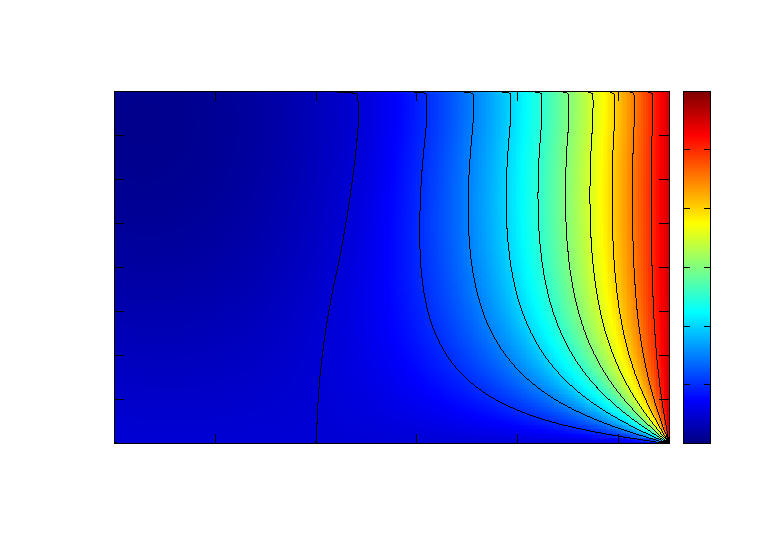
\includegraphics{FourMaterials/Resultats5000}}%
    \gplfronttext
  \end{picture}%
\endgroup

	\caption{Instantaneous isotherms at t=5000 s}
	\label{plot4M}
\end{figure}

Since the temperature in the right wall changes over time, the four materials problem never reaches a steady state. However, to see the evolution of the temperature, the simulation has been  run for a final time of $t=10000 s$, obtaining the results of the figure \ref{4Mfinal}.
\begin{figure}[h]
	\centering
	% GNUPLOT: LaTeX picture with Postscript
\begingroup
  \makeatletter
  \providecommand\color[2][]{%
    \GenericError{(gnuplot) \space\space\space\@spaces}{%
      Package color not loaded in conjunction with
      terminal option `colourtext'%
    }{See the gnuplot documentation for explanation.%
    }{Either use 'blacktext' in gnuplot or load the package
      color.sty in LaTeX.}%
    \renewcommand\color[2][]{}%
  }%
  \providecommand\includegraphics[2][]{%
    \GenericError{(gnuplot) \space\space\space\@spaces}{%
      Package graphicx or graphics not loaded%
    }{See the gnuplot documentation for explanation.%
    }{The gnuplot epslatex terminal needs graphicx.sty or graphics.sty.}%
    \renewcommand\includegraphics[2][]{}%
  }%
  \providecommand\rotatebox[2]{#2}%
  \@ifundefined{ifGPcolor}{%
    \newif\ifGPcolor
    \GPcolortrue
  }{}%
  \@ifundefined{ifGPblacktext}{%
    \newif\ifGPblacktext
    \GPblacktexttrue
  }{}%
  % define a \g@addto@macro without @ in the name:
  \let\gplgaddtomacro\g@addto@macro
  % define empty templates for all commands taking text:
  \gdef\gplbacktext{}%
  \gdef\gplfronttext{}%
  \makeatother
  \ifGPblacktext
    % no textcolor at all
    \def\colorrgb#1{}%
    \def\colorgray#1{}%
  \else
    % gray or color?
    \ifGPcolor
      \def\colorrgb#1{\color[rgb]{#1}}%
      \def\colorgray#1{\color[gray]{#1}}%
      \expandafter\def\csname LTw\endcsname{\color{white}}%
      \expandafter\def\csname LTb\endcsname{\color{black}}%
      \expandafter\def\csname LTa\endcsname{\color{black}}%
      \expandafter\def\csname LT0\endcsname{\color[rgb]{1,0,0}}%
      \expandafter\def\csname LT1\endcsname{\color[rgb]{0,1,0}}%
      \expandafter\def\csname LT2\endcsname{\color[rgb]{0,0,1}}%
      \expandafter\def\csname LT3\endcsname{\color[rgb]{1,0,1}}%
      \expandafter\def\csname LT4\endcsname{\color[rgb]{0,1,1}}%
      \expandafter\def\csname LT5\endcsname{\color[rgb]{1,1,0}}%
      \expandafter\def\csname LT6\endcsname{\color[rgb]{0,0,0}}%
      \expandafter\def\csname LT7\endcsname{\color[rgb]{1,0.3,0}}%
      \expandafter\def\csname LT8\endcsname{\color[rgb]{0.5,0.5,0.5}}%
    \else
      % gray
      \def\colorrgb#1{\color{black}}%
      \def\colorgray#1{\color[gray]{#1}}%
      \expandafter\def\csname LTw\endcsname{\color{white}}%
      \expandafter\def\csname LTb\endcsname{\color{black}}%
      \expandafter\def\csname LTa\endcsname{\color{black}}%
      \expandafter\def\csname LT0\endcsname{\color{black}}%
      \expandafter\def\csname LT1\endcsname{\color{black}}%
      \expandafter\def\csname LT2\endcsname{\color{black}}%
      \expandafter\def\csname LT3\endcsname{\color{black}}%
      \expandafter\def\csname LT4\endcsname{\color{black}}%
      \expandafter\def\csname LT5\endcsname{\color{black}}%
      \expandafter\def\csname LT6\endcsname{\color{black}}%
      \expandafter\def\csname LT7\endcsname{\color{black}}%
      \expandafter\def\csname LT8\endcsname{\color{black}}%
    \fi
  \fi
    \setlength{\unitlength}{0.0500bp}%
    \ifx\gptboxheight\undefined%
      \newlength{\gptboxheight}%
      \newlength{\gptboxwidth}%
      \newsavebox{\gptboxtext}%
    \fi%
    \setlength{\fboxrule}{0.5pt}%
    \setlength{\fboxsep}{1pt}%
\begin{picture}(7200.00,5040.00)%
    \gplgaddtomacro\gplbacktext{%
    }%
    \gplgaddtomacro\gplfronttext{%
      \put(936,624){\makebox(0,0){\strut{}$0$}}%
      \put(1905,624){\makebox(0,0){\strut{}$0.2$}}%
      \put(2874,624){\makebox(0,0){\strut{}$0.4$}}%
      \put(3842,624){\makebox(0,0){\strut{}$0.6$}}%
      \put(4811,624){\makebox(0,0){\strut{}$0.8$}}%
      \put(5780,624){\makebox(0,0){\strut{}$1$}}%
      \put(748,938){\makebox(0,0)[r]{\strut{}$0$}}%
      \put(748,1361){\makebox(0,0)[r]{\strut{}$0.1$}}%
      \put(748,1784){\makebox(0,0)[r]{\strut{}$0.2$}}%
      \put(748,2207){\makebox(0,0)[r]{\strut{}$0.3$}}%
      \put(748,2630){\makebox(0,0)[r]{\strut{}$0.4$}}%
      \put(748,3053){\makebox(0,0)[r]{\strut{}$0.5$}}%
      \put(748,3476){\makebox(0,0)[r]{\strut{}$0.6$}}%
      \put(748,3899){\makebox(0,0)[r]{\strut{}$0.7$}}%
      \put(748,4322){\makebox(0,0)[r]{\strut{}$0.8$}}%
      \put(6796,938){\makebox(0,0)[l]{\strut{}$20$}}%
      \put(6796,1361){\makebox(0,0)[l]{\strut{}$25$}}%
      \put(6796,1784){\makebox(0,0)[l]{\strut{}$30$}}%
      \put(6796,2207){\makebox(0,0)[l]{\strut{}$35$}}%
      \put(6796,2630){\makebox(0,0)[l]{\strut{}$40$}}%
      \put(6796,3053){\makebox(0,0)[l]{\strut{}$45$}}%
      \put(6796,3476){\makebox(0,0)[l]{\strut{}$50$}}%
      \put(6796,3899){\makebox(0,0)[l]{\strut{}$55$}}%
      \put(6796,4322){\makebox(0,0)[l]{\strut{}$60$}}%
    }%
    \gplbacktext
    \put(0,0){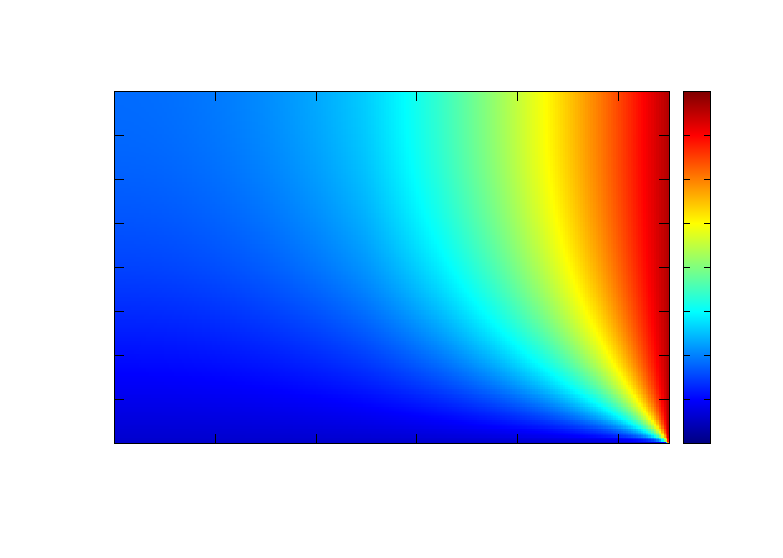
\includegraphics{FourMaterials/Resultats}}%
    \gplfronttext
  \end{picture}%
\endgroup

	\caption{Instantaneous plot at t=10000 s}
	\label{4Mfinal}
\end{figure}

Comparing the solutions at 5000 s and at 10000 s, it can be seen that the whole rod has increased its temperature, but the gradient of temperature between the left and right walls has doubled. Another important difference is that hot temperatures move to the left as time passes.

In addition, to further analyse the results obtained, the same simulation has been run for two rods of homogeneous material. The geometrical parameters and the boundary conditions have been maintained, but the physical properties of the whole material are those of the section $M_{2}$ (figure \ref{HomoM2}) and $M_{3}$ (figure \ref{HomoM3}) respectively of the four materials problem.
\begin{figure}[h]
	\centering
	% GNUPLOT: LaTeX picture with Postscript
\begingroup
  \makeatletter
  \providecommand\color[2][]{%
    \GenericError{(gnuplot) \space\space\space\@spaces}{%
      Package color not loaded in conjunction with
      terminal option `colourtext'%
    }{See the gnuplot documentation for explanation.%
    }{Either use 'blacktext' in gnuplot or load the package
      color.sty in LaTeX.}%
    \renewcommand\color[2][]{}%
  }%
  \providecommand\includegraphics[2][]{%
    \GenericError{(gnuplot) \space\space\space\@spaces}{%
      Package graphicx or graphics not loaded%
    }{See the gnuplot documentation for explanation.%
    }{The gnuplot epslatex terminal needs graphicx.sty or graphics.sty.}%
    \renewcommand\includegraphics[2][]{}%
  }%
  \providecommand\rotatebox[2]{#2}%
  \@ifundefined{ifGPcolor}{%
    \newif\ifGPcolor
    \GPcolortrue
  }{}%
  \@ifundefined{ifGPblacktext}{%
    \newif\ifGPblacktext
    \GPblacktexttrue
  }{}%
  % define a \g@addto@macro without @ in the name:
  \let\gplgaddtomacro\g@addto@macro
  % define empty templates for all commands taking text:
  \gdef\gplbacktext{}%
  \gdef\gplfronttext{}%
  \makeatother
  \ifGPblacktext
    % no textcolor at all
    \def\colorrgb#1{}%
    \def\colorgray#1{}%
  \else
    % gray or color?
    \ifGPcolor
      \def\colorrgb#1{\color[rgb]{#1}}%
      \def\colorgray#1{\color[gray]{#1}}%
      \expandafter\def\csname LTw\endcsname{\color{white}}%
      \expandafter\def\csname LTb\endcsname{\color{black}}%
      \expandafter\def\csname LTa\endcsname{\color{black}}%
      \expandafter\def\csname LT0\endcsname{\color[rgb]{1,0,0}}%
      \expandafter\def\csname LT1\endcsname{\color[rgb]{0,1,0}}%
      \expandafter\def\csname LT2\endcsname{\color[rgb]{0,0,1}}%
      \expandafter\def\csname LT3\endcsname{\color[rgb]{1,0,1}}%
      \expandafter\def\csname LT4\endcsname{\color[rgb]{0,1,1}}%
      \expandafter\def\csname LT5\endcsname{\color[rgb]{1,1,0}}%
      \expandafter\def\csname LT6\endcsname{\color[rgb]{0,0,0}}%
      \expandafter\def\csname LT7\endcsname{\color[rgb]{1,0.3,0}}%
      \expandafter\def\csname LT8\endcsname{\color[rgb]{0.5,0.5,0.5}}%
    \else
      % gray
      \def\colorrgb#1{\color{black}}%
      \def\colorgray#1{\color[gray]{#1}}%
      \expandafter\def\csname LTw\endcsname{\color{white}}%
      \expandafter\def\csname LTb\endcsname{\color{black}}%
      \expandafter\def\csname LTa\endcsname{\color{black}}%
      \expandafter\def\csname LT0\endcsname{\color{black}}%
      \expandafter\def\csname LT1\endcsname{\color{black}}%
      \expandafter\def\csname LT2\endcsname{\color{black}}%
      \expandafter\def\csname LT3\endcsname{\color{black}}%
      \expandafter\def\csname LT4\endcsname{\color{black}}%
      \expandafter\def\csname LT5\endcsname{\color{black}}%
      \expandafter\def\csname LT6\endcsname{\color{black}}%
      \expandafter\def\csname LT7\endcsname{\color{black}}%
      \expandafter\def\csname LT8\endcsname{\color{black}}%
    \fi
  \fi
    \setlength{\unitlength}{0.0500bp}%
    \ifx\gptboxheight\undefined%
      \newlength{\gptboxheight}%
      \newlength{\gptboxwidth}%
      \newsavebox{\gptboxtext}%
    \fi%
    \setlength{\fboxrule}{0.5pt}%
    \setlength{\fboxsep}{1pt}%
\begin{picture}(7200.00,5040.00)%
    \gplgaddtomacro\gplbacktext{%
    }%
    \gplgaddtomacro\gplfronttext{%
      \put(1273,624){\makebox(0,0){\strut{}$0$}}%
      \put(2119,624){\makebox(0,0){\strut{}$0.2$}}%
      \put(2966,624){\makebox(0,0){\strut{}$0.4$}}%
      \put(3811,624){\makebox(0,0){\strut{}$0.6$}}%
      \put(4658,624){\makebox(0,0){\strut{}$0.8$}}%
      \put(5504,624){\makebox(0,0){\strut{}$1$}}%
      \put(1085,938){\makebox(0,0)[r]{\strut{}$0$}}%
      \put(1085,1361){\makebox(0,0)[r]{\strut{}$0.1$}}%
      \put(1085,1784){\makebox(0,0)[r]{\strut{}$0.2$}}%
      \put(1085,2207){\makebox(0,0)[r]{\strut{}$0.3$}}%
      \put(1085,2630){\makebox(0,0)[r]{\strut{}$0.4$}}%
      \put(1085,3053){\makebox(0,0)[r]{\strut{}$0.5$}}%
      \put(1085,3476){\makebox(0,0)[r]{\strut{}$0.6$}}%
      \put(1085,3899){\makebox(0,0)[r]{\strut{}$0.7$}}%
      \put(1085,4322){\makebox(0,0)[r]{\strut{}$0.8$}}%
      \put(6408,938){\makebox(0,0)[l]{\strut{}$15$}}%
      \put(6408,1314){\makebox(0,0)[l]{\strut{}$20$}}%
      \put(6408,1690){\makebox(0,0)[l]{\strut{}$25$}}%
      \put(6408,2066){\makebox(0,0)[l]{\strut{}$30$}}%
      \put(6408,2442){\makebox(0,0)[l]{\strut{}$35$}}%
      \put(6408,2818){\makebox(0,0)[l]{\strut{}$40$}}%
      \put(6408,3194){\makebox(0,0)[l]{\strut{}$45$}}%
      \put(6408,3570){\makebox(0,0)[l]{\strut{}$50$}}%
      \put(6408,3946){\makebox(0,0)[l]{\strut{}$55$}}%
      \put(6408,4322){\makebox(0,0)[l]{\strut{}$60$}}%
    }%
    \gplbacktext
    \put(0,0){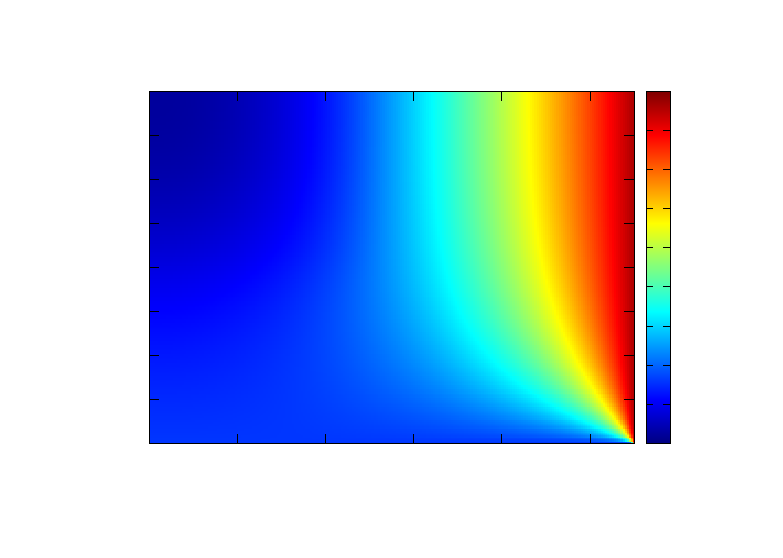
\includegraphics{FourMaterials/HomoM2}}%
    \gplfronttext
  \end{picture}%
\endgroup

	\caption{Instantaneous plot at t=10000 s for the homogeneous material $M_{2}$}
	\label{HomoM2}
\end{figure}
\begin{figure}[h]
	\centering
	% GNUPLOT: LaTeX picture with Postscript
\begingroup
  \makeatletter
  \providecommand\color[2][]{%
    \GenericError{(gnuplot) \space\space\space\@spaces}{%
      Package color not loaded in conjunction with
      terminal option `colourtext'%
    }{See the gnuplot documentation for explanation.%
    }{Either use 'blacktext' in gnuplot or load the package
      color.sty in LaTeX.}%
    \renewcommand\color[2][]{}%
  }%
  \providecommand\includegraphics[2][]{%
    \GenericError{(gnuplot) \space\space\space\@spaces}{%
      Package graphicx or graphics not loaded%
    }{See the gnuplot documentation for explanation.%
    }{The gnuplot epslatex terminal needs graphicx.sty or graphics.sty.}%
    \renewcommand\includegraphics[2][]{}%
  }%
  \providecommand\rotatebox[2]{#2}%
  \@ifundefined{ifGPcolor}{%
    \newif\ifGPcolor
    \GPcolortrue
  }{}%
  \@ifundefined{ifGPblacktext}{%
    \newif\ifGPblacktext
    \GPblacktexttrue
  }{}%
  % define a \g@addto@macro without @ in the name:
  \let\gplgaddtomacro\g@addto@macro
  % define empty templates for all commands taking text:
  \gdef\gplbacktext{}%
  \gdef\gplfronttext{}%
  \makeatother
  \ifGPblacktext
    % no textcolor at all
    \def\colorrgb#1{}%
    \def\colorgray#1{}%
  \else
    % gray or color?
    \ifGPcolor
      \def\colorrgb#1{\color[rgb]{#1}}%
      \def\colorgray#1{\color[gray]{#1}}%
      \expandafter\def\csname LTw\endcsname{\color{white}}%
      \expandafter\def\csname LTb\endcsname{\color{black}}%
      \expandafter\def\csname LTa\endcsname{\color{black}}%
      \expandafter\def\csname LT0\endcsname{\color[rgb]{1,0,0}}%
      \expandafter\def\csname LT1\endcsname{\color[rgb]{0,1,0}}%
      \expandafter\def\csname LT2\endcsname{\color[rgb]{0,0,1}}%
      \expandafter\def\csname LT3\endcsname{\color[rgb]{1,0,1}}%
      \expandafter\def\csname LT4\endcsname{\color[rgb]{0,1,1}}%
      \expandafter\def\csname LT5\endcsname{\color[rgb]{1,1,0}}%
      \expandafter\def\csname LT6\endcsname{\color[rgb]{0,0,0}}%
      \expandafter\def\csname LT7\endcsname{\color[rgb]{1,0.3,0}}%
      \expandafter\def\csname LT8\endcsname{\color[rgb]{0.5,0.5,0.5}}%
    \else
      % gray
      \def\colorrgb#1{\color{black}}%
      \def\colorgray#1{\color[gray]{#1}}%
      \expandafter\def\csname LTw\endcsname{\color{white}}%
      \expandafter\def\csname LTb\endcsname{\color{black}}%
      \expandafter\def\csname LTa\endcsname{\color{black}}%
      \expandafter\def\csname LT0\endcsname{\color{black}}%
      \expandafter\def\csname LT1\endcsname{\color{black}}%
      \expandafter\def\csname LT2\endcsname{\color{black}}%
      \expandafter\def\csname LT3\endcsname{\color{black}}%
      \expandafter\def\csname LT4\endcsname{\color{black}}%
      \expandafter\def\csname LT5\endcsname{\color{black}}%
      \expandafter\def\csname LT6\endcsname{\color{black}}%
      \expandafter\def\csname LT7\endcsname{\color{black}}%
      \expandafter\def\csname LT8\endcsname{\color{black}}%
    \fi
  \fi
    \setlength{\unitlength}{0.0500bp}%
    \ifx\gptboxheight\undefined%
      \newlength{\gptboxheight}%
      \newlength{\gptboxwidth}%
      \newsavebox{\gptboxtext}%
    \fi%
    \setlength{\fboxrule}{0.5pt}%
    \setlength{\fboxsep}{1pt}%
\begin{picture}(7200.00,5040.00)%
    \gplgaddtomacro\gplbacktext{%
    }%
    \gplgaddtomacro\gplfronttext{%
      \put(1273,624){\makebox(0,0){\strut{}$0$}}%
      \put(2119,624){\makebox(0,0){\strut{}$0.2$}}%
      \put(2966,624){\makebox(0,0){\strut{}$0.4$}}%
      \put(3811,624){\makebox(0,0){\strut{}$0.6$}}%
      \put(4658,624){\makebox(0,0){\strut{}$0.8$}}%
      \put(5504,624){\makebox(0,0){\strut{}$1$}}%
      \put(1085,938){\makebox(0,0)[r]{\strut{}$0$}}%
      \put(1085,1361){\makebox(0,0)[r]{\strut{}$0.1$}}%
      \put(1085,1784){\makebox(0,0)[r]{\strut{}$0.2$}}%
      \put(1085,2207){\makebox(0,0)[r]{\strut{}$0.3$}}%
      \put(1085,2630){\makebox(0,0)[r]{\strut{}$0.4$}}%
      \put(1085,3053){\makebox(0,0)[r]{\strut{}$0.5$}}%
      \put(1085,3476){\makebox(0,0)[r]{\strut{}$0.6$}}%
      \put(1085,3899){\makebox(0,0)[r]{\strut{}$0.7$}}%
      \put(1085,4322){\makebox(0,0)[r]{\strut{}$0.8$}}%
      \put(6408,938){\makebox(0,0)[l]{\strut{}$20$}}%
      \put(6408,1361){\makebox(0,0)[l]{\strut{}$25$}}%
      \put(6408,1784){\makebox(0,0)[l]{\strut{}$30$}}%
      \put(6408,2207){\makebox(0,0)[l]{\strut{}$35$}}%
      \put(6408,2630){\makebox(0,0)[l]{\strut{}$40$}}%
      \put(6408,3053){\makebox(0,0)[l]{\strut{}$45$}}%
      \put(6408,3476){\makebox(0,0)[l]{\strut{}$50$}}%
      \put(6408,3899){\makebox(0,0)[l]{\strut{}$55$}}%
      \put(6408,4322){\makebox(0,0)[l]{\strut{}$60$}}%
    }%
    \gplbacktext
    \put(0,0){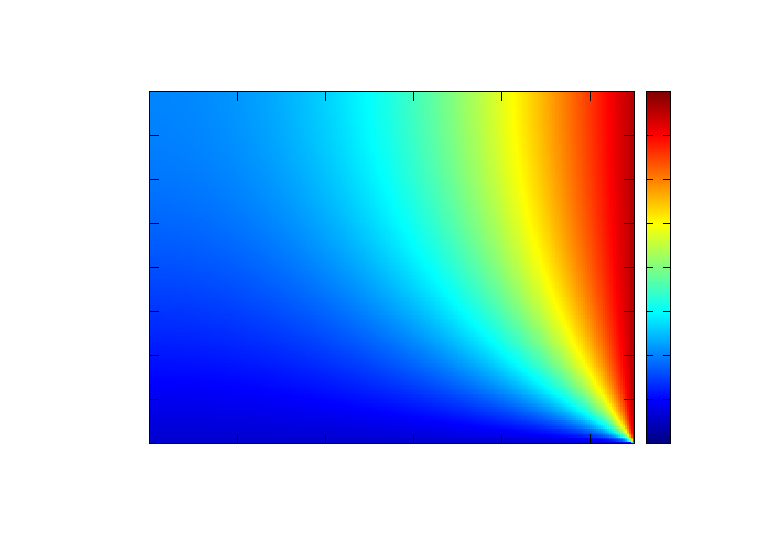
\includegraphics{FourMaterials/HomoM3}}%
    \gplfronttext
  \end{picture}%
\endgroup

	\caption{Instantaneous plot at t=10000 s for the homogeneous material $M_{3}$}
	\label{HomoM3}
\end{figure}

Comparing the graphs, it can be stated that the final result is very similar in all three cases. In the case of the $M_{2}$ material, the main visible difference is that in the four materials problem, higher temperatures move further to the left. In the original problem, the upper right region is made of the material $M_{4}$, which has the same conductivity as the homogeneous material $M_{2}$, but a higher density and specific heat.

In the case of the homogeneous $M_{3}$ material, it can be seen that it is the material that has better conductivity, because hotter temperatures move slightly further to the left in the upper zone compared to the results of the original problem.